\chapter{fondamenti}
\section{logica}

Se, come diceva Galileo, la matematica è il linguaggio della natura,
è importante che la matematica sia essa stessa espressa in un linguaggio
che risulti essere il più possibile oggettivo e non ambiguo.
La \emph{logica} è la disciplina matematica che si occupa
dello studio e della formalizzazione del linguaggio matematico.
In questo capitolo riassumiamo in maniera sintetica ed intuitiva
alcuni concetti e contemporaneamente
fissiamo le notazioni che verranno utilizzate nel seguito.

La logica studia i \emph{sistemi formali}%
\mymargin{sistemi formali}%
\index{sistemi formali} (anche detti \emph{sistemi logico-deduttivi}
o \emph{sistemi assiomatici)} che sono delle descrizioni meccaniche, non ambigue, 
di un linguaggio formale. 
Parliamo al plurale di \emph{sistemi formali} in quanto ogni ambito della matematica 
(o di altre scienze) potrebbe sviluppare un proprio sistema formale specializzato per quell'ambito. 
Il primo sistema formale è stato sviluppato da Euclide per descrivere le proprietà 
di punti, rette e circonferenze del piano (la \emph{geometria euclidea}).
Al tempo di Euclide la formalizzazione era ancora intuitiva e incompleta, 
la formalizzazione moderna 
di tale sistema è stata completata da Hilbert, dopo duemila anni.
Peano ha introdotto un sistema assiomatico per descrivere le proprietà dei numeri naturali.
Dedekind ha individuato gli assiomi per descrivere i numeri reali.
Cantor ha introdotto la \emph{teoria degli insiemi} all'interno della quale è stato 
possibile includere tutte le altre teorie matematiche. 
Tale teoria è stata formalizzata da Zermelo e Fraenkel
ed è questa la teoria che useremo nel nostro corso.

Tutti sistemi formali descrivono un linguaggio.
Per descrivere un linguaggio dobbiamo dire innanzitutto quali sono i \emph{simboli}%
\mymargin{simboli}%
\index{simboli}
di quel linguaggio. In generale possiamo pensare ai simboli come alle lettere 
(o caratteri, nel linguaggio dell'informatica) che possono essere utilizzati per comporre le frasi.
Simboli tipici delle teorie matematiche sono ad esempio: 
\texttt{x}, \texttt{y}, \texttt{5}, \texttt{7}, 
\texttt{+}, \texttt{=}, \texttt{)}, \texttt{:} etc.
Nei linguaggi informatici i simboli corrispondono ai caratteri presenti sulla tastiera 
di un computer. 
Nelle lingue naturali si prenderebbero come simboli le singole lettere dell'alfabeto
a cui aggiungere eventualmente i caratteri per la punteggiatura.
Una sequenza finita di simboli si chiama \emph{formula}%
\mymargin{formula}%
\index{formula} (potremmo anche chiamarle \emph{frasi}).
Ad esempio: \texttt{x7)+} potrebbe essere una formula formata da quattro simboli.
Tra tutte le formule un sistema formale deve individuare quelle che si potrebbero chiamare 
\emph{formule ben formate} ovvero le formule a cui effettivamente vogliamo dare significato.
Ad esempio la formula $x+5=7$ potrebbe essere una formula ben formata perché siamo in grado 
di dargli un significato.
Il sistema formale non dà un significato alle formule ben formate 
(il significato è una estrapolazione della nostra mente) ma semplicemente deve dare delle regole 
per determinare quali siano le formule ben formate e quali no.
Visto che ogni simbolo che utilizziamo può essere rappresentato al computer, possiamo pensare 
alle formule come alle stringhe dei linguaggi di programmazione e possiamo pensare che il sistema formale 
deve descrivere un algoritmo (cioè un procedimento meccanico) in grado di determinare 
se una formula è ben formata oppure no.
Tra le \emph{formule ben formate} il sistema formale deve infine specificare quali 
siano i \emph{teoremi}. 
Di nuovo questo deve essere fatto mediante un algoritmo puramente meccanico 
in modo da garantire che i teoremi risultino oggettivi e universali: 
non ci può essere disaccordo sulla validità di un teorema, eventualmente 
ci può essere disaccordo 
sulla interpretazione di tale teorema.
Tipicamente i sistemi formali sono \emph{deduttivi}.
Nei sistemi \emph{deduttivi} si identificano alcune formule che vengono 
chiamate
 \emph{assiomi} e che vengono immediatamente riconosciuti come teoremi.
Ad esempio vedremo che il primo assioma della teoria degli insiemi è 
\[
  \exists X\colon \not \exists y\colon y\in X
\]
che si potrebbe leggere 
\begin{displayquote}
esiste un insieme $X$ per il quale nessun $y$ è elemento di $X$
\end{displayquote}
ed esprime l'esistenza dell'insieme vuoto.
Oltre agli assiomi in un sistema deduttivo vengono specificate delle 
\emph{regole di inferenza} cioè dei modi in cui 
le formule possono essere modificate o composte in modo tale che se le formule 
di partenza sono teoremi anche la formula ottenuta lo è.
I \emph{sillogismi} di Aristotele possono essere utilizzati come esempi di regole 
di inferenza. 
Supponiamo che le formule 
\texttt{"Socrate è un uomo"} 
e \texttt{"l'uomo è un animale"}
siano entrambe teoremi. Allora possiamo pensare di definire una regola di inferenza 
che mi dice che se \texttt{"X è un Y"} è un teorema 
e \texttt{"Y è uno Z"}
è un teorema allora anche \texttt{"X è uno Z"} è un teorema. 
Con questa regola di inferenza è quindi possibile dedurre che 
\texttt{"Socrate è un animale"}
è un teorema.
E' chiaro che se le regole formali possono essere definite meccanicamente 
tramite un algoritmo allora anche i teoremi possono essere determinati meccanicamente 
mediante un algoritmo.
La ricerca in matematica consiste nell'esplorare lo spazio delle formule ben formate 
per determinare quali siano effettivamente teoremi. 
Dare la \emph{dimostrazione}%
\mymargin{dimostrazione}%
\index{dimostrazione} di un teorema significa esibire tutta la catena delle formule 
e delle regole di inferenza che permettono di ottenere il teorema a partire dagli 
assiomi.

\subsection{proposizioni, operatori logici}

Tutto questo è un processo meccanico, ma in realtà è ovvio che i sistemi formali 
vengono definiti in modo tale da aver per noi un qualche tipo di significato intuitivo.
In tal modo la ricerca delle dimostrazioni non è un processo puramente meccanico 
ma segue delle linee di pensiero che possono richiedere intuizione, inventiva e anche 
senso estetico. 
Tipicamente a livello intuitivo vogliamo assegnare un valore di verità alle formule 
ben formate: vorremmo cioè dire che alcune formule sono 
\emph{vere}%
\mymargin{vero}%
\index{vere} 
ed altre sono 
\emph{false}%
\mymargin{falso}%
\index{false}. 
In tal caso le formule ben formate vengono usualmente chiamate \emph{proposizioni}%
\mymargin{proposizioni}%
\index{proposizione}
(nel linguaggio naturale diremmo: \emph{affermazioni}).
Un esempio di proposizione (falsa) potrebbe essere: 
\texttt{2+2=5}.

E' possibile combinare più proposizioni mediante
gli operatori logici. Se $P$ e $Q$ sono proposizioni
si può costruire la proposizione $P \land Q$
chiamata \emph{congiunzione logica}%
\mymargin{congiunzione}%
\index{congiunzione logica}.
Tale proposizione
si può leggere ``$P$ e $Q$'' ed è una proposizione
che risulta essere vera solamente nel caso in cui sia
$P$ che $Q$ siano vere
(si veda la tabella~\ref{tab:verita_operatori_logici}
per un riassunto schematico).
Spesso la congiunzione logica è sottointesa:
se si fa un elenco di proposizioni $P,Q,R$ 
si intende usualmente la loro congiunzione $P \land Q \land R$
cioè si intende che devono essere tutte vere.
La \emph{disgiunzione logica}%
\mymargin{disgiunzione}%
\index{disgiunzione logica} denotata
con $P \lor Q$
si può leggere ``$P$ o $Q$'' ed è una proposizione che
è vera se almeno una tra $P$ e $Q$ è vera.
La \emph{negazione logica}%
\mymargin{negazione}%
\index{negazione logica} denotata con $\lnot P$ è una
proposizione che si può leggere ``non $P$'' che
è vera quando $P$ è falsa ed è falsa quando $P$ è vera.

Operatori logici molto utilizzati sono le \emph{implicazioni}%
\mymargin{implicazioni}%
\index{implicazione}.
La proposizione $P\Rightarrow Q$ si può leggere ``$P$ implica $Q$''
e significa che $Q$ è vera se $P$ è vera. Non si confonda
il valore di verità di $P\Rightarrow Q$ con il valore di verità
di $Q$. Se $P$ è vera allora $P\Rightarrow Q$ è vera o falsa
a seconda che $Q$ sia vera o falsa. Ma se $P$ è falsa allora
l'implicazione $P\Rightarrow Q$ è vera indipendentemente dal
valore di $Q$. In effetti $P\Rightarrow Q$ è equivalente a
$Q \lor \lnot P$ perché per la verità di $P\Rightarrow Q$
basta che $Q$ sia vera (quando $P$ è vera) oppure che $P$ sia falsa.

La freccia inversa $P\Leftarrow Q$ si può utilizzare per
invertire l'implicazione: è equivalente a $Q \Rightarrow P$.
Se valgono entrambe le implicazioni
$(P \Leftarrow Q) \land (P\Rightarrow Q)$
è facile convincersi che $P$ e $Q$ devono avere lo stesso
valore di verità: diremo quindi che sono equivalenti e
scriveremo $P \Leftrightarrow Q$.

Nella tabella~\ref{tab:verita_operatori_logici} sono riportati
tutti i valori di verità che si possono ottenere combinando
tra loro due proposizioni. Nella tabella~\ref{tab:operatori_logici}
sono riportate alcune proprietà di tali operatori: queste
proprietà possono essere comprese interpretando il loro significato
ma possono anche essere dedotte meccanicamente. 
Per verificare meccanicamente la validità di una di queste 
espressioni logiche è sufficiente fare una tabella in cui si 
inseriscono tutti i possibili valori di verità di $P$, $Q$ ed $R$
(in totale saranno $8$ casi) e per ognuno di questi si dovrà
calcolare il valore di verità di ogni operazione svolta e verificare 
che ogni espressione completa assume il valore $V$ (vero).
Diremo che queste sono \emph{tautologie}
\index{tautologia}%
\mymargin{tautologia}%
ovvero espressioni logiche la cui validità non dipende
dal valore di verità dei suoi termini.

\begin{table}
\begin{center}
  \begin{tabular}{cc|cccccc}
    $P$ & $Q$ & $\neg P$ & $P\land Q$ & $P\lor Q$ & $P\Rightarrow Q$ &
    $P\Leftarrow Q$ & $P\Leftrightarrow Q$ \\\hline
    \texttt{F} & \texttt{F} & \texttt{V} & \texttt{F} & \texttt{F} & \texttt{V} & \texttt{V} & \texttt{V} \\
    \texttt{F} & \texttt{V} & \texttt{V} & \texttt{F} & \texttt{V} & \texttt{V} & \texttt{F} & \texttt{F} \\
    \texttt{V} & \texttt{F} & \texttt{F} & \texttt{F} & \texttt{V} & \texttt{F} & \texttt{V} & \texttt{F} \\
    \texttt{V} & \texttt{V} & \texttt{F} & \texttt{V} & \texttt{V} & \texttt{V} & \texttt{V} & \texttt{V} \\
    \end{tabular}
\end{center}
\caption{La tabella di verità degli operatori logici. 
$\texttt{F}$ significa \emph{falso}, $\texttt{V}$ significa \emph{vero}.}
\label{tab:verita_operatori_logici}
\end{table}

\begin{table}
\begin{tabular}{rcll}
                          &$\neg (P \land \neg P)$&                              & non contraddizione \\
                         &$P \lor \neg P$&                                       & terzo escluso \\
                         $\neg \neg P$ & $\iff$ & $ P$                           & doppia negazione\\
                                    $P \land Q$ & $\iff$ & $ Q \land P$                   & simmetria\\
                                     $P \lor Q$ & $\iff$ & $ Q \lor P$                    & \\
                              $\neg (P\land Q)$ & $\iff$ & $ (\neg P) \lor (\neg Q)$      & formule di De Morgan\\
                               $\neg (P\lor Q)$ & $\iff$ & $ (\neg P) \land (\neg Q)$     & \\
                            $(P\land Q) \lor R$ & $\iff$ & $ (P\lor R) \land (Q \lor R)$  & proprietà distributiva\\
                            $(P\lor Q) \land R$ & $\iff$ & $ (P\land R) \lor (Q \land R)$ & \\
                            $(P \Rightarrow Q)$ & $\iff$ & $ (Q \Leftarrow P)$            & antisimmetria\\
                            $(P\Rightarrow Q)$ & $\iff$ & $ (\neg Q\Rightarrow\neg P)$   & implicazione contropositiva\\
                        $\neg (P\Rightarrow Q)$ & $\iff$ & $ P \land (\neg Q)$            & controesempio\\
                             $P\Rightarrow Q$ & $\iff$ & $ \lnot(P \land (\neg Q))$     & dimostrazione per assurdo
\end{tabular}
\caption{Alcune proprietà degli operatori logici. Queste proposizioni sono tutte vere qualunque siano i valori di verità delle proposizioni $P$ e $Q$. In particolare le equivalenze logiche ci dicono che le proposizioni ai due lati dell'equivalenza assumono sempre lo stesso valore di verità e quindi sono interscambiabili.}
\label{tab:operatori_logici}
\end{table}

Per definire formalmente la logica del calcolo proposizionale
dobbiamo avere un sistema sottostante che ci dice chi sono 
le proposizioni di base, ovvero i termini che possiamo sostituire al posto 
di $P$, $Q$, $R$. 
Queste saranno proposizioni (ovvero formule ben formate).
Una volta definite le proposizioni di base,
ogni formula della forma
$(P)\land(Q)$, $(P)\lor(Q)$, $(P)\implies(Q)$, 
$(P)\impliedby (Q)$, $(P)\Leftrightarrow(Q)$ e
$\lnot(P)$
è anch'essa una proposizione (ovvero è ben formata) 
se $P$ e $Q$ lo sono. 
Il sistema formale utilizza i simboli: 
$\land$ $\lor$ $\implies$ $\impliedby$ $\Leftrightarrow$
$\lnot$ $($ $)$ oltre a tutti i simboli che servono per 
comporre le proposizioni di base.

Il caso più semplice possibile è quello in cui abbiamo 
solamente due proposizioni di base $F$ e $V$ e due assiomi: 
$V$ e $\lnot (F)$. 
In questo sistema possiamo prendere $V$ e $\lnot (F)$ 
come assiomi.
L'interpretazione del sistema è che $V$ è vero mentre $F$ è falso.

Le regole di inferenza del calcolo delle proposizioni
possono essere date in modi diversi. 
\index{regole di inferenza}%
\mymargin{regole di inferenza}%
Proviamo a spiegare (senza troppi formalismi) il sistema 
che viene chiamato \emph{deduzione naturale}. 
Questo sistema presenta per ognuno degli operatori logici
(negazione, congiunzione, disgiunzione, implicazione) 
due regole formali: una che permette l'introduzione l'operatore e una 
che permette l'eliminazione l'operatore.

Le regole più semplici sono quelle che riguardano la congiunzione 
logica. Se $P$ e $Q$ sono teoremi possiamo dedurre che anche 
$(P)\land (Q)$ è un teorema (introduzione della congiunzione).
\index{congiunzione logica}%
\index{introduzione!congiunzione}%
\mymargin{introduzione congiunzione}%
Viceversa se $(P)\land (Q)$ è un teorema possiamo dedurre 
che sia $P$ che $Q$ sono teoremi (eliminazione della congiunzione).
\index{eliminazione!congiunzione}%
\mymargin{eliminazione congiunzione}%
Ad esempio se abbiamo il teorema $1+1=2$ e il teorema $2+1=3$ 
allora possiamo dedurre che $(1+1=2) \land (2+1=3)$ è un teorema.
Viceversa se $(1+1=2)\land (2+1=3)$ è un teorema allora possiamo 
dedurre che $2+1=3$ è un teorema.

Anche l'introduzione della disgiunzione logica è una regola 
\index{disgiunzione logica}%
molto semplice: se $P$ è un teorema allora anche $(P)\lor (Q)$ 
e $(Q)\lor (P)$ sono teoremi, qualunque sia la proposizione $Q$.
\index{introduzione disgiunzione}%
\mymargin{introduzione disgiunzione}%
Ad esempio se $1+1=2$ è un teorema possiamo dedurre 
che anche $(1+1=2) \lor (1+1\neq 2)$ è un teorema.
La regola di eliminazione della disgiunzione è leggermente 
\mymargin{eliminazione disgiunzione}%
più complicata. Se  $(P)\lor (Q)$ è un teorema e se entrambi 
$(P)\implies (R)$ e $(Q)\implies (R)$ sono teoremi, possiamo 
dedurre che $R$ è un teorema.
Ad esempio se abbiamo i teoremi: 
\[
\begin{gathered}
  (x>1) \implies (x^2>1)\\ 
  (x<-1) \implies (x^2>1)\\  
  (x>1) \lor (x<-1)
\end{gathered}
\]
allora possiamo dedurre che $x^2>1$ 
è un teorema.

Per quanto riguarda l'implicazione logica, la regola di eliminazione 
\index{implicazione logica}%
si chiama \emph{modus ponens} ed è forse la più importante 
\index{modus ponens}%
\mymargin{modus ponens}%
delle regole di inferenza.
La regola ci dice che se abbiamo il teorema 
$P$ e il teorema $(P)\implies (Q)$ possiamo affernare che anche 
$Q$ è un teorema.
Ad esempio se abbiamo dimostrato $(1+1=2) \implies (2+1=3)$ 
e abbiamo dimostrato $1+1=2$ allora possiamo dedurre $2+1=3$.
Questa regola formale dà significato all'implicazione logica.

La regola di \emph{introduzione della implicazione} è più complicata 
\mymargin{introduzione implicazione}%
da formalizzare e richiede l'introduzione di un nuovo concetto:
il \emph{contesto} dimostrativo.
\index{contesto dimostrativo}%
\mymargin{contesto dimostrativo}%
Un \emph{contesto} è in pratica un nuovo sistema formale che 
eredita tutti gli assiomi e le regole formali del sistema formale 
originario ma con delle proprietà in più che permettono tipicamente di 
ottenere teoremi che non era possibile ottenere nel sistema formale 
originale.
Per l'introduzione dell'implicazione logica la regola 
è la seguente. Per poter affermare che $(P)\implies (Q)$ 
è un teorema introduciamo un nuovo contesto in cui 
tutti i teoremi già dimostrati sono assiomi e inoltre 
anche $P$ è un assioma aggiuntivo. 
Se in questo contesto riusciamo ad ottenere $Q$ come
teorema allora possiamo dire che $(P)\implies (Q)$ è un teorema 
nel sistema formale originale.
Si noti che $Q$ potrebbe non essere un teorema nel contesto 
orginale, lo è solo nel contesto ipotetico in cui abbiamo 
supposto (per ipotesi, appunto) che $P$ fosse un teorema.

Proviamo per esempio a dimostrare la regola più controversa
delle tavole di verità ovvero
che $F\implies V$ (dove $F$ sta per falso e 
$V$ sta per vero). 
Quello che dobbiamo fare è verificare che se $\lnot P$ 
è un teorema (cioè $P$ è falso) e se se $Q$ è un teorema 
(cioè $Q$ è vero) allora $P\implies Q$ è un teorema.
Dovremmo usare la regola di introduzione dell'implicazione logica.
Dunque supponiamo per ipotesi che $P$ sia un teorema. 
Visto che $Q$ era un teorema nel contesto originale 
$Q$ rimane un teorema nel contesto ipotetico in cui 
abbiamo supposto che $P$ sia un assioma.
Possiamo quindi, fuori dal contesto, dedurre $P\implies Q$ 
come volevasi dimostrare.

Ad esempio al posto di $P$ possiamo mettere $1\neq 1$ 
e al $Q$ possiamo mettere $1=1$. 
Vorremo allora dimostrare che $1\neq 1 \implies 1=1$ 
è un teorema.
Proviamo a farlo formalmente con tutti i dettagli.

Supponiamo di avere un sistema formale 
contenente i simboli $1$, $2$, $=$, $\neq$ oltre che
tutti i simboli della logica proposizionale 
(ovvero $\land$, $\lor$, $\lnot$, $\implies$, $($ e $)$).
Chiamiamo \emph{costanti} i simboli $1$ e $2$.
Supponiamo che tutte le formule della forma 
$x\neq y$ e $x=y$ siano proposizioni 
(formule ben formate) se al posto di $x$ e $y$ 
mettiamo qualunque costante. 
Supponiamo che $x\neq y$ sia un sinonimo di $\lnot x=y$,
Supponiamo infine che $x=x$ sia un assioma se al posto 
di $x$ mettiamo qualunque costante.

Fuori dal sistema formale, nell'esibire una dimostrazione,
faremo un elenco dei nostri teoremi, numerando ogni riga 
per poterci fare riferimento. 
Usiamo le parentesi graffe $\{$ e $\}$ per racchiudere 
i contesti dimostrativi. 
Tra parentesi quadre indichiamo le regole formali che stiamo 
utilizzando. 
\begin{theorem}[esempio di dimostrazione formale]
  $2 \neq 2 \implies 1=1$.
\end{theorem}
%  
\begin{proof}
  \begin{align}
    &\{ & &\text{[inizio contesto ipotetico]} \\ 
    &\quad 2\neq 2 & & \text{[ipotesi]}  \\
    &\quad 1=1 & & \text{[assioma]} \\
    &\} & & \text{[fine del contesto ipotetico]} \\
    &2\neq 2 \implies 1=1 & & \text{[introduzione implicazione]}
  \end{align}
\end{proof}

% Ad esempio possiamo dimostrare che 
% $1=2 \implies (2=3 \implies 1=3)$.
% Si inizia con l'introdurre un contesto ipotetico in cui $1=2$.
% In questo contesto introduciamo un nuovo \emph{sotto}-contesto 
% in cui anche $2=3$. Nel sotto-contesto abbiamo come teoremi
% (ipotetici) sia $1=2$ che $2=3$. 
% Un assioma dell'uguaglianza (che non abbiamo ancora menzionato)
% permetterà di dire che se $x=y$ allora in un qualunque teorema 
% si possono rimpiazzare le occorrenze di $x$ con $y$ e viceversa.
% Dunque se (ipoteticamente) $1=2$ e $2=3$ possiamo rimpiazzare 
% $2$ con $1$ nell'uguaglianza $2=3$ per ottenere $1=3$.
% Si noti che $1=3$ è falso. 
% Ma sarebbe effettivamente un teorema nell'ipotesi (assurda)
% che $1=2$ e $2=3$.
% Dunque possiamo dedurre $2=3 \implies 1=3$ nel contesto 
% in cui abbiamo ipotizzato $1=2$. 
% E possiamo dedurre $1=2 \implies (2=3 \implies 1=3)$ nel
% contesto generale. Quest'ultimo è un vero e proprio teorema,
% valido senza ipotesi aggiuntive.

Ritorniamo alle regole di inferenza del calcolo proposizionale.

Veniamo infine alla negazione logica. 
\index{negazione logica}%
\mymargin{rimozione negazione}%
Per la rimozione la regola è quella della doppia negazione: 
se $\lnot (\lnot (P))$ è un teorema allora anche $P$ è un teorema.
Ad esempio se $\lnot (\lnot (1=1))$ è un teorema allora anche $1=1$ 
è un teorema.
\mymargin{introduzione negazione}%
La regola di introduzione della negazione logica è la 
dimostrazione per assurdo.
\index{dimostrazione!per assurdo}%
\index{assurdo!dimostrazione per}%
Se introduciamo un contesto formale in cui assumiamo (per assurdo)
che $P$ sia un teorema e, nel contesto, riusciamo ad ottenere 
una contraddizione (ad esempio $\lnot (P)$) allora possiamo 
affermare che (fuori dal contesto) $\lnot (P)$ è un teorema.

Ad esempio se $1=1$ è un teorema possiamo dimostrare 
che anche $\lnot \lnot (1=1)$ è un teorema.
Infatti supponiamo per assurdo $\lnot \lnot \lnot (1=1)$.
Allora, tramite eliminazione della doppia negazione possiamo 
dedurre $\lnot (1=1)$. Ma questo è in contraddizione 
con $\lnot \lnot (1=1)$. Dunque abbiamo dimostrato che 
$\lnot \lnot (1=1)$.

Le regole formali che abbiamo introdotto sono sufficienti 
per dimostrare la validità delle tabelle di verità degli 
operatori logici.

\begin{exercise}
Si provino ad utilizzare le regole formali di inferenza del 
calcolo proposizionale per dimostrare la validità delle 
tavole di verità.
\end{exercise}

\subsection{predicati, quantificatori}

Un \emph{predicato}%
\mymargin{predicato}%
\index{predicato} è una proposizione che contiene
una o più variabili il cui valore di verità, quindi,
può dipendere dal valore assegnato alle variabili.
Un esempio di predicato è $x+2=5$ che risulta essere vero se $x=3$
e falso altrimenti.

Le variabili $x,y,\dots$ non sono altro che simboli 
del sistema formale. 
Usualmente vengono utilizzate le ultime lettere dell'alfabeto.
Siccome le lettere dell'alfabeto sono in numero finito
e visto che vogliamo invece avere la possibilità di introdurre 
sempre nuove variabili, decidiamo che 
una variabile può essere composta da una sequenza di più simboli. 
Si può ad esempio usare l'apice: $x$, $x'$, $x''$ oppure 
usare una sequenza di lettere: $\textrm{area}$, $\sin$
per avere una quantità illimitata di nomi diversi a disposizione.

Se un predicato dipende da una o più variabili queste
si chiamano \emph{variabili libere}%
\mymargin{variabili libere}%
\index{variabili libere}. E' possibile
\emph{chiudere} una variabile libera mediante un quantificatore.
Il \emph{quantificatore universale}%
\mymargin{quantificatore universale}%
\index{quantificatore universale} denotato col simbolo
$\forall$ serve ad affermare che il predicato è vero
per ogni possibile valore della variabile quantificata.
Ad esempio la proposizione $\forall x\colon x+2=5$ significa:
``per ogni $x$ si ha $x+2=5$'' ed è una proposizione falsa.
Il quantificatore $\forall x$ rende \emph{muta} la variabile
$x$ del predicato $x+2=5$ nel senso che il valore di verità 
della proposizione
non dipende più dal valore di quella variabile, che non è
più una variabile libera ma funge solo da segnaposto.
In effetti se cambio nome ad una variabile muta il valore 
di verità non cambia. Ad esempio scrivere $\forall x\colon x+1=1+x$
è equivalente a $\forall z\colon z+1=1+z$.

Il \emph{quantificatore esistenziale}%
\mymargin{quantificatore esistenziale}%
\index{quantificatore esistenziale} denotato col simbolo
$\exists$ serve ad affermare che il predicato è vero per
almeno un valore della variabile quantificata.
Ad esempio la proposizione $\exists x\colon x+2=5$ significa:
``esiste almeno un $x$ per cui risulta $x+2=5$''.
Quello che si ottiene è una proposizione in cui la variabile
$x$ è muta. In questo caso la proposizione è vera in quanto
per $x=3$ il predicato è vero.

Un predicato può dipendere da più variabili ed è quindi
possibile inserire più quantificatori. In tal caso l'ordine
dei quantificatori può essere rilevante.
Delle seguenti proposizioni la prima è vera, la seconda
invece è falsa:
\begin{gather*}
\forall x\colon \exists y\colon x+2=y \\
\exists y\colon \forall x\colon x+2=y.
\end{gather*}
Intuitivamente la prima affermazione ci dice che per ogni numero $x$ 
esiste un numero $y$ che differisce di $2$ da $x$.
La seconda ci dice che c'è un numero $y$ che differisce di $2$ 
da qualunque numero $x$.

\begin{table}
  \begin{center}
    \begin{tabular}{lcl}
    $\lnot \forall x \colon P(x)$ & $\iff$ & $\exists x \colon \lnot P(x)$\\
    $\lnot \exists x \colon P(x)$ & $\iff$ & $\forall x \colon \lnot P(x)$\\
    \end{tabular}
  \end{center}
  \caption{Le formule di De Morgan per i quantificatori logici.}
  \label{tab:proprieta_quantificatori}
\end{table}

Risulta utile saper trasformare un quantificatore logico
nell'altro per mezzo delle negazioni con le formule 
di De Morgan riportate
nella tabella~\ref{tab:proprieta_quantificatori}.

Spesso il quantificatore universale viene sottointeso.
Ad esempio se si scrive $x+y=y+x$
si intende che tutte le variabili libere sono quantificate 
tramite quantificatore universale: 
$\forall x\colon \forall y\colon x+y=y+x$.
Il segno di interpunzione $\colon$ può essere omesso
e una quantificazione può essere fatta contemporaneamente 
su più variabili. 
Potremo quindi scrivere: $\forall x\forall y\colon x+y=y+x$ 
o anche $\forall x,y\colon x+y = y+x$.
A volte, se non crea ambiguità, si potranno scrivere 
i quantificatori anche a fine frase 
\[
  x+y=y+x \quad \forall x\forall y.
\]

Una proposizione non può contenere variabili libere, 
altrimenti il suo valore di verità potrebbe dipendere da quelle 
variabili e non sarebbe quindi ben definito.
\mymargin{costanti}%
\index{costanti}%
Si può però intendere che alcune variabili sono \emph{costanti},
cioè rappresentano un oggetto ben preciso.
Ad esempio nella proposizione $\forall x: \pi > -x^2$ si intende 
che $\pi$ è una costante, ovvero un ben preciso numero.
Anche le cifre $0$, $1$, $2$ sono usualmente sempre intese come
costanti.

Insieme al calcolo dei predicati si introduce usualmente anche il simbolo di uguaglianza \texttt{=}.
Come viene definita l'uguaglianza dipende da come sono definiti gli oggetti trattati 
dal nostro sistema formale, cosa che noi faremo per la teoria degli insiemi nel prossimo paragrafo.
Ma comunque venga definita l'uguaglianza si richiede che valga il seguente.
\begin{axiom}[uguaglianza]
\[
  \forall x\colon x=x.  
\]
\end{axiom}
Inoltre si richiede che oggetti uguali possano essere 
sostituiti uno all'altro in un teorema:
se $x=y$ e $P(x)$ sono teoremi allora anche $P(y)$ lo è.

Anche per il calcolo dei predicati dobbiamo specificare le regole 
di inferenza per l'introduzione e l'eliminazione dei quantificatori.

\mymargin{eliminazione $\forall$}%
\index{quantificatore!universale}%
L'eliminazione del quantificatore universale è molto semplice. 
Se abbiamo un teorema della forma $\forall x\colon P(x)$
e se nel contesto dimostrativo è stata introdotta una costante 
$c$, allora possiamo dedurre $P(c)$.
\mymargin{introduzione $\forall$}%
Viceversa, per introdurre il quantificatore universale 
dobbiamo aprire un contesto dimostrativo in cui supponiamo 
che $x$ sia una costante di cui non abbiamo alcuna informazione 
(cioè $x$ non è usata come costante al di fuori del contesto).
Se nel contesto riusciamo a dimostrarare una proposizione $P(x)$ possiamo 
allora dedurre, fuori contesto, il teorema $\forall x\colon P(x)$.

In pratica si dirà: fissato $x$ qualunque, abbiamo dimostrato $P(x)$
quindi possiamo affermare che $\forall x\colon P(x)$.

\index{quantificatore!esistenziale}%
\mymargin{eliminazione $\exists$}%
Per quanto riguarda il quantificatore esistenziale la regola 
di eliminazione ci dice che se abbiamo un teorema della forma 
$\exists x\colon P(x)$ possiamo introdurre un contesto dimostrativo 
in cui è definita una costante $c$ che ha la proprietà $P(c)$.
\mymargin{introduzione $\exists$}%
Viceversa, se abbiamo un teorema della forma $P(c)$ 
possiamo dedurre $\exists x\colon P(x)$.

Come esempio enunciamo e dimostriamo formalmente un semplice 
teorema.

\begin{theorem}[esempio di dimostrazione formale]
  \[ \forall x \exists y\colon x=y \]
\end{theorem}
\begin{proof}
  \begin{align}
    &\forall x\colon x = x & & \text{[assioma]} \label{ff1}\\
    &\{ & &\text{[fissiamo $x$ qualunque]}\\
    &\quad x=x  & & \text{[eliminazione $\forall$ da \eqref{ff1}]}\\ 
    &\quad \exists y\colon x=y & &\text{[introduzione $\exists$]}\\
    &\} & &\\
    &\forall x\exists y\colon x=y & &\text{[introduzione $\forall$]} 
  \end{align}
\end{proof}

\section{teoria degli insiemi}

Nei paragrafi precedenti abbiamo visto che i predicati possono essere
combinati tra loro e quantificati.
Ma quali sono i predicati elementari che possiamo considerare per fondare 
tutta la matematica?
La teoria degli insiemi ci fornisce la formalizzazione del concetto
di \emph{appartenenza}: il predicato di base (l'unico che ci servirà) è
un predicato della forma $x \in A$ che significa ``l'oggetto $x$ è un elemento
dell'insieme $A$''.
La teoria degli insiemi non spiega (né tantomento definisce)
cosa siano gli oggetti e cosa siano gli insiemi perché questi sono concetti
primitivi (come lo sono i \emph{punti} e le \emph{rette} per la geometria euclidea).
La teoria degli insiemi ci fornisce, semplicemente, le regole formali che
possono essere utilizzate per trattare i predicati della forma $x\in A$.
Ad esempio un \emph{assioma} 
della teoria degli insiemi è il seguente.
\begin{axiom}[insieme vuoto]
\[
  \exists A \colon \lnot \exists x\colon x \in A
\]
\end{axiom}
L'assioma significa: ``esiste un insieme $A$ che non contiene alcun elemento $x$''
ovvero stiamo dicendo che esiste l'\emph{insieme vuoto}%
\mymargin{insieme vuoto}%
\index{insieme vuoto} che normalmente viene
denotato con il simbolo $\emptyset$.
Scriveremo quindi $\exists\emptyset\colon \forall x\colon \lnot(x\in \emptyset)$.
Possiamo quindi introdurre un contesto dimostrativo 
in cui $\emptyset$ è una costante e l'assioma diventa più
semplicemente $\forall x\colon \lnot (x\in \emptyset)$.

Altri opportuni assiomi della teoria degli insiemi garantiscono l'esistenza
dell'unione $A\cup B$, intersezione $A\cap B$ e differenza $A\setminus B$
di due insiemi qualunque $A$ e $B$. Tali operazioni
tra insiemi possono essere ricondotte alla relazione di appartenenza
e possono quindi essere definite come segue.

\begin{axiom}[operazioni tra insiemi]
Se $A$ e $B$ sono insiemi allora esistono gli insiemi  
$U=A\cup B$ (unione), $I=A\cap B$ (intersezione) e 
$D=A\setminus B$ (differenza).
\mymargin{unione intersezione differenza}%
\index{unione}%
\index{intersezione}%
\index{differenza}%
Formalmente:
\begin{align*}
    \forall A,B\colon \exists U\colon \forall x\colon x\in U &\iff (x\in A) \lor (x\in B),\\
    \forall A,B\colon \exists I\colon \forall x\colon x\in I &\iff (x\in A) \land (x\in B),\\
    \forall A,B\colon \exists D\colon \forall x\colon x\in D &\iff (x\in A) \land \lnot (x \in B).
\end{align*}
\end{axiom}

La negazione dell'appartenenza $\lnot (x \in A)$ viene usualmente
abbreviata con $x \not \in A$.

Sempre utilizzando la semplice relazione di appartenenza possiamo definire
le relazioni di inclusione e uguaglianza tra insiemi:
$A \subset B$ si legge ``$A$ è un sottoinsieme di $B$'',
$A \supset B$ si legge ``$A$ è un sovrainsieme di $B$''
e $A=B$ si legge ``$A$ è uguale a $B$''. 
Queste relazioni sono definite dalle seguenti proprietà:
\begin{align*}
  A \subset B &\iff \forall x\colon (x\in A \implies x\in B)\\
  A \supset B &\iff \forall x\colon (x\in A \implied x\in B)\\
  A = B &\iff \forall x\colon (x\in A \iff x \in B).
\end{align*}
A parole diremo che $A$ è un sottoinsieme di $B$, 
$A \subset B$, se ogni elemento di $A$ è anche elemento di $B$.
Diremo che $A$ e $B$ sono uguali, $A=B$, 
se $A$ e $B$ hanno gli stessi elementi.
Ovviamente la relazione $\supset$ non è altro 
che la relazione inversa di $\subset$ cioè risulta 
$A\supset B$ se e solo se $B\subset A$.
Scriveremo anche $A \neq B$ per indicare
la relazione opposta dell'uguaglianza ovvero: $\lnot(A=B)$.
Si noti che $A=B$ è equivalente a $(A\subset B) \land (B\subset A)$.

% In molti sistemi formali l'uguaglianza è un predicato primitivo con la 
% proprietà che oggetti uguali possono essere sostituiti uno all'altro 
% in ogni proposizione. Per recuperare tale proprietà 
% dobbiamo imporre il seguente.
% 
% \begin{axiom}[estensionalità]
% Se $x=y$ allora il predicato $x\in A$ è equivalente 
% al predicato $y\in A$.
% \end{axiom}

La relazione $A \subset B$ significa che ogni elemento di $A$ 
è anche elemento di $B$ e quindi non ci sono elementi di $A$ che non stiano 
in $B$ cioè $A$ non è più grande di $B$. 
Come stratagemma mnemonico si osservi che il simbolo 
$\subset$ è orientato in modo che l'insieme più piccolo 
stia dal lato più stretto della relazione così come 
nella disuguaglianza $3 \le 5$ il numero più piccolo 
sta dal lato più stretto del simbolo $\le$.
Per dimostrare che la relazione $A \subset B$ è vera 
bisognerà prendere un qualunque elemento di $A$ e dimostrare 
che tale elemento è anche elemento di $B$.
Per dimostrare che vale l'uguaglianza $A=B$ tipicamente si procede 
dimostrando separatamente le due inclusioni $A\subset B$ e $B\subset A$.

Risulta molto utile la possibilità di costruire insiemi di insiemi.
Per questo motivo la teoria degli insiemi usualmente non fa distinzione
tra oggetti e insiemi di oggetti. Nella relazione primitiva $x\in A$ anche
$x$ può essere un insieme. Possiamo allora immaginare che ogni oggetto del
nostro universo sia un insieme. In questo modo la relazione di uguaglianza $A=B$
che abbiamo definito sopra risulta ben definita per ogni coppia di oggetti
(o insiemi, che è lo stesso) $A$ e $B$.

Visto che gli elementi di un insieme $\mathcal A$ sono a loro volta insiemi,
è possibile considerare l'unione $\bigcup \mathcal A$
e, se\mynote{%
L'intersezione di una famiglia vuota di insiemi darebbe l'insieme 
universo, che vedremo non può essere definito.
} 
$\mathcal A \neq \emptyset$, l'intersezione $\bigcap \mathcal A$ di tutti gli elementi
di $\mathcal A$.
Questo estende il concetto di unione e intersezione anche a famiglie
eventualmente infinite.

\begin{axiom}[unione e intersezione arbitraria]
Se $\mathcal A$ è un insieme qualunque esiste l'insieme $\bigcup \mathcal A$
e se $\mathcal A \neq \emptyset$ esiste l'insieme $\bigcap \mathcal A$
con le seguenti proprietà:
\begin{align*}
  x \in \bigcup \mathcal A & \iff \exists A \in \mathcal A \colon x\in A, \\
  x \in \bigcap \mathcal A & \iff \forall A \in \mathcal A \colon x\in A.
\end{align*}
\end{axiom}
Una notazione alternativa è la seguente:
\[
 \bigcup \mathcal A = \bigcup_{A\in \mathcal A} A, \qquad 
 \bigcap \mathcal A = \bigcap_{A\in \mathcal A} A.  
\]
Questa notazione mette in evidenza il fatto che l'insieme 
$\bigcup \mathcal A$ è l'unione di tutti gli elementi $A$ dell'insieme 
$\mathcal A$ mentre $\bigcap \mathcal A$ è l'intersezione 
di tutti gli elementi di $\mathcal A$.
L'insieme $\mathcal A$ viene spesso chiamata una \emph{famiglia}
di insiemi perché i suoi elementi vengono trattati come insiemi 
più che come oggetti.

Un altro assioma della teoria degli insiemi garantisce che per ogni
$x$ esiste un insieme il cui unico elemento è $x$. 
\begin{axiom}[singoletto]
  Se $x$ è un insieme esiste l'insieme $\ENCLOSE{x}$, 
  chiamato \emph{singoletto}%
\mymargin{singoletto}%
\index{singoletto}
  tale che:
  \[
    y \in \ENCLOSE{x} \iff y=x.
  \]
\end{axiom}
Facendo l'unione di singoletti possiamo definire (per elencazione) insiemi che contengono
un numero finito di oggetti:
\begin{align*}
  \ENCLOSE{a,b} &= \ENCLOSE{a} \cup \ENCLOSE{b} \\
  \ENCLOSE{a, b, c} &= \ENCLOSE{a,b} \cup \ENCLOSE{c}\\
  \ENCLOSE{a, b, c, d} &= \ENCLOSE{a,b,c} \cup \ENCLOSE{d}\\
  &\quad\vdots
\end{align*}

Si faccia però attenzione: l'insieme $\ENCLOSE{a,b}$ contiene due elementi
solamente se $a\neq b$, infatti se $a=b$ si potrà facilmente verificare
che
\begin{equation}\label{eq:4775523}
\ENCLOSE{a,a} = \ENCLOSE{a}.
\end{equation}

\begin{exercise}
  Verificare \eqref{eq:4775523} utilizzando le definizioni formali date in precedenza.
\end{exercise}
\begin{proof}[Svolgimento.]
Utilizzando le definizioni di unione, di singoletto e di disgiunzione logica
si ha l'equivalenza dei seguenti
predicati:
\begin{gather*}
  x \in \ENCLOSE{a,a}  \\
  x \in \ENCLOSE{a} \cup \ENCLOSE{a}\\
  (x \in \ENCLOSE{a}) \lor (x \in \ENCLOSE{a})\\
  (x = a) \lor (x = a) \\
  x = a \\
  x \in \ENCLOSE{a}
\end{gather*}
e dunque $\ENCLOSE{a,a}=\ENCLOSE{a}$ per la definizione di uguaglianza tra insiemi.
\end{proof}

Se $P(x)$ è un predicato in una sola variabile $x$ vorremmo poter
definire l'insieme di tutti gli oggetti $x$ 
che rendono vero il predicato $P$.
Sorprendentemente se aggiungessimo questo assioma 
(chiamato assioma di specificazione ingenua) nella teoria degli insiemi
avremmo un paradosso%
\index{teoria!ingenua degli insiemi}%
\index{insiemi!teoria ingenua}%
\index{Cantor, Georg}%
\index{Frege}%
\index{Russell}%
\mynote{Georg Cantor (1845--1918), Bertrand Russell (1872--1970) 
vedi note storiche a pag.~\pageref{nota:Cantor}}.

\begin{theorem}[paradosso di Russell]
\label{th:Russell}%
Non esiste un insieme $R$ tale che per ogni $x$ si abbia
\[
   x\in R \iff x\not \in x
\]
(un tale insieme si potrebbe definire così
tramite un assioma di specificazione \emph{ingenua}: $R=\ENCLOSE{x\colon x\not \in x}$).
\end{theorem}
%
\begin{proof}
  Se esistesse avremmo:
  \[
    R \in R 
    \iff R\not \in R
  \]
  e questo è in contrasto
  con il principio di non contraddizione
  (un predicato e la sua negazione non possono essere entrambi veri).
\end{proof}

Per evitare l'incoerenza è necessario limitare l'\emph{assioma di specificazione}
alla costruzione di sottoinsiemi di insiemi già costruiti.

\begin{axiom}[specificazione]
  Se $P$ è un qualunque predicato con una variabile libera $x$
  e se $B$ è un insieme, allora esiste l'insieme 
  $\ENCLOSE {x\in B\colon P(x)}$ formato 
  da tutti gli elementi di $B$ che soddisfano il predicato $P$:
\[
  a \in \ENCLOSE{x\in B\colon P(x)} \iff (a \in B \land P(a)).
\]
\end{axiom}

Se ora proviamo a ripetere il ragionamento di Russell dato un insieme $A$ 
possiamo costruire l'insieme $R=\ENCLOSE{x\in A\colon x\not \in x}$
e scopriremmo che non può essere $R\in R$ 
(altrimenti dovrebbe essere $R\not \in R$ assurdo).
Ma potrebbe benissimo essere $R\not \in R$ se inoltre $R\not \in A$.
Dunque si deduce che dato qualunque insieme $A$ c'è un insieme 
che non è elemento di $A$: dobbiamo quindi rassegnarci al fatto che non
esiste un insieme \emph{universo} contenente qualunque altro insieme,
ma almeno non otteniamo una contraddizione%
\mynote{%
D'altra parte non possiamo comunque escludere che una contraddizione 
esista. 
Infatti Goedel ha dimostrato che non è possibile dimostrare che 
non ci siano contraddizioni nel sistema assiomatico da noi considerato.
}.

Per completare la teoria degli insiemi introduciamo anche il concetto di
\emph{insieme delle parti}%
\mymargin{insieme delle parti}%
\index{insieme!delle parti}
\index{$\mathcal P(\cdot)$}% 
cioè l'insieme di tutti i sottoinsiemi di un insieme dato.
\begin{axiom}[insieme delle parti]
\label{def:insieme_parti}%
Se $A$ è un insieme esiste l'insieme $\P(A)$ delle parti di $A$
che è l'insieme di tutti i sottoinsiemi di $A$:
\begin{equation}\label{eq:insieme_delle_parti}
  x \in \mathcal P(A) \iff x \subset A.
\end{equation}
\end{axiom}

\subsection{gli ordinali finiti di Von Neumann}

Con i soli assiomi che abbiamo introdotto fin'ora possiamo 
costruire un numero arbitrariamente grande di insiemi finiti
tramite una costruzione dovuta a Von Neumann. 
Possiamo definire 
$0=\emptyset$, $1= 0 \cup \ENCLOSE{0}$, $2=1\cup \ENCLOSE{1}$,
$3 = 2\cup \ENCLOSE{2}$, $4=3\cup\ENCLOSE{3}$ e $5=4\cup \ENCLOSE{4}$.
Esplicitando queste definizioni si osserva che:
$0 = \ENCLOSE{}$ è un insieme con zero elementi, 
$1= \ENCLOSE{0}$ è un insieme con un elemento (lo zero),
$2= \ENCLOSE{0,1}$ è un insieme con due elementi (i due precedenti), 
$3 = \ENCLOSE{0,1,2}$ è un insieme con tre elementi (i tre precedenti),
etc.
Procedendo a piacere è possibile definire un numero arbitrariamente 
grande di insiemi finiti, uno diverso dall'altro.

Questi particolari insiemi esistono certamente e potremo quindi utilizzarli 
nel seguito per fare esempi di insiemi finiti.
E' anche possibile (ma non necessario) utilizzare questi insiemi 
per definire i numeri naturali (si veda l'assioma di infinito, più avanti).

\begin{exercise}
Verificare che $0\in 1 \in 2 \in 3 \in 4 \in 5$, 
che $0\subset 1 \subset 2 \subset 3 \subset 4 \subset 5$ 
e che $0\neq 1$, $0\neq 2$, $1\neq 2$, etc.
\end{exercise}

\subsection{relazioni}

Grazie agli assiomi precedenti è possibile definire il prodotto cartesiano
di due insiemi: sarà questo un concetto molto importante nel seguito.
Innanzitutto dobbiamo definire il concetto di \emph{coppia}%
\mymargin{coppia}%
\index{coppia}: dati
$a,b$ definiamo la coppia $(a,b)$ con primo elemento $a$ e secondo elemento $b$
come un oggetto che ha questa proprietà:%
\mynote{%
Un modo formale per definire la coppia tramite l'utilizzo di insiemi 
è dovuto a Kuratowski:
\[
   (a,b) = \ENCLOSE{\ENCLOSE{a},\ENCLOSE{a,b}}.
\]
Non è difficile verificare che questa definizione soddisfa la 
proprietà~\eqref{eq:coppia}.
Così possiamo definire l'insieme prodotto
\begin{align*}
  A\times B = \big\{&C\in \mathcal P(\mathcal P(A\cup B))\colon \\ 
  & \exists a\colon \exists b\colon a\in A, b\in B, \\
  & C=\ENCLOSE{\ENCLOSE{a},\ENCLOSE{a,b}}\big\}
\end{align*}
}%
\begin{equation}\label{eq:coppia}
  (a, b) = (a', b') \iff (a=a') \land (b=b').
\end{equation}
Stiamo cioè richiedendo che una coppia venga identificata dai due
elementi che la compongono in cui, però, è importante anche l'ordine in
cui vengono elencati (a differenza dell'insieme $\ENCLOSE{a,b}$, in cui
l'ordine degli elementi è irrilevante).
Nel seguito useremo anche la notazione $a \mapsto b$ per indicare 
la coppia $(a,b)$ e la chiameremo \emph{freccia}%
\mymargin{freccia}%
\index{freccia} da $a$ in $b$.

Il \emph{prodotto cartesiano} $A\times B$ di due insiemi $A$ e $B$
è l'insieme di tutte le coppie
il cui primo elemento sta in $A$ e
il secondo elemento sta in $B$:
\[
  (a, b) \in A \times B \iff (a\in A \land b\in B).
\]

Se rappresentiamo gli elementi di $A$ come dei punti su una retta
orizzontale (asse delle $x$) e gli elementi di $B$ come dei punti
su una retta verticale (asse delle $y$) gli elementi di $A\times B$
possono essere rappresentati come i punti del piano che proiettati sull'asse
delle $x$ vanno in $A$ e proiettati sull'asse delle $y$ vanno in $B$
(si veda la figura~\ref{fig:funzione}). 
  
Una \emph{relazione}%
\mymargin{relazione}%
\index{relazione} $R$ tra gli elementi di un insieme $A$ e gli elementi
di un insieme $B$ non è altro che un sottoinsieme di $A\times B$
ovvero $R\in \mathcal P(A\times B)$.
Per una relazione $R\subset A\times B$ si userà la notazione infissa
$aRb$ per indicare $(a,b)\in R$.
Oppure con la notazione delle freccie potremo 
scrivere $a \stackrel R \mapsto b$
per indicare che la freccia $a\mapsto b$ è un elemento di $R$. 
Ad esempio se prendo $A=B=\ENCLOSE{1,2,3}$ e considero la relazione 
$R=\ENCLOSE{(1,2),(1,3),(2,3)}$
il predicato $aRb$ rappresenta l'usuale relazione d'ordine $a<b$ sui
tre numeri considerati.

\begin{definition}[relazione di equivalenza]
\label{def:equivalenza}%
Sia $R\subset A\times A$ una relazione sull'insieme $A$. Diremo che 
$R$ è una \emph{relazione di equivalenza}%
\mymargin{relazione di equivalenza}%
\index{relazione!di equivalenza} se valgono le seguenti proprietà
(tipiche dell'uguaglianza)
per ogni $x,y,z\in A$:
\begin{enumerate}
  \item riflessiva: $x R x$;
  \item simmetrica: se $x R y$ allora $y R x$;
  \item transitiva: se $x R y$ e $yRz$ allora $x R z$.
\end{enumerate}
Se $R$ è una relazione di equivalenza diremo che $x$ è equivalente a $y$ 
(tramite $R$) quando $xRy$.
Dato $x \in A$ l'insieme di tutti gli elementi $y\in A$ che sono equivalenti 
a $x$ si chiama \emph{classe di equivalenza}%
\mymargin{classe di equivalenza}%
\index{classe!di equivalenza} di $x$. 
Si definisce in questo modo:
\[
  [x]_R = \ENCLOSE{y\in A \colon xRy}.  
\]
Se $R$ è una relazione di equivalenza su $A$ definiamo 
l'\emph{insieme quoziente}
\mymargin{insieme quoziente}%
\index{insieme!quoziente}%
$A/R$
come l'insieme di tutte le classi di equivalenza:
\[
 A/R 
 = \ENCLOSE{[x]_R\colon x\in A} 
 = \ENCLOSE{B\in \mathcal P(A)\colon \exists x\in A\colon B=[x]_R}.  
\]
\end{definition}

Se $R$ è una relazione di equivalenza su $A$ 
l'insieme quoziente $A/R$ rappresenta l'insieme 
degli oggetti di $A$ in cui vengono identificati tra loro gli oggetti tra loro 
equivalenti.
Spesso diremo che $A/R$ rappresenta $A$ a meno della equivalenza $R$.

Ad esempio se $A=\ENCLOSE{1,2,3,4,5}$ e prendiamo $D=\ENCLOSE{1,3,5}$ (i numeri dispari)
e $P=\ENCLOSE{2,4}=A\setminus D$ 
(i numeri pari) possiamo definire una relazione $R$ su $A$ mediante la proprietà:
\[
 x R  y \iff (x\in P \land y\in P) \lor (x\in D \land y\in D).
\]
La relazione $R$ rappresenta la proprietà degli elementi di $A$ 
di avere la stessa ``parità''. 
Si avrà $[1]_R = [3]_R=[5]_R= D$ e $[2]_R=[4]_R=P$.
Dunque 
\[
   A/R = \ENCLOSE{P,D} = \ENCLOSE{\ENCLOSE{2,4},\ENCLOSE{1,3,5}}
\]
e, in effetti, questo insieme ha due elementi $P$ e $D$ che è quello 
che si ottiene identificando i numeri di $A$ in base alla proprietà 
di essere pari o dispari. 

L'insieme quoziente $A/R$ è un \emph{partizione}%
\mymargin{partizione}%
\index{partizione} di $A$ in quanto 
è formato da insiemi disgiunti la cui unione è tutto $A$. In effetti 
dare una partizione di $A$ è equivalente da dare una relazione 
di equivalenza.

\subsection{funzioni}

Sia $f$ una relazione tra due insiemi $A$ e $B$. 
Useremo la notazione delle frecce quindi scriveremo $a\stackrel f\mapsto b$ 
se $(a,b)\in f$. 
Diremo che $f$ è una funzione da $A$ in $B$ e scriveremo 
$f\colon A\to B$ se per ogni $a\in A$ esiste un unico $b\in B$ 
tale che $a \stackrel f \mapsto b$.
Potremmo dire che $f$ è definita su $A$ 
(perché per ogni punto di $A$ c'è una freccia)
ed è univoca (perché tale freccia è unica).

Dato $a\in A$ esiste dunque un unico $b\in B$ tale che
$a\stackrel f \mapsto b$: chiameremo $fa$
o $f(a)$ 
\mymargin{$f(x)$}%
tale oggetto $b$
e diremo che la funzione $f$ manda $a$ in $b$. 
Si avrà dunque
\[
 b=f(a) \iff a\stackrel f \mapsto b.
\]
Gli elementi del dominio spesso vengono chiamati \emph{punti}
mentre gli elementi del codominio, se sono numeri, vengono 
chiamati \emph{valori}. 
La funzione $f$ avrà quindi valore $f(a)$ nel punto $a$.
L'insieme di tutte le funzioni $f\colon A\to B$ viene usualmente denotato $B^A$
oppure $A\to B$.
\mymargin{$B^A$}%
\index{$A^B$}%
\index{$A\to B$}%
\index{potenza!insiemi}%

\begin{figure}
  \mbox{}
  \hfill
  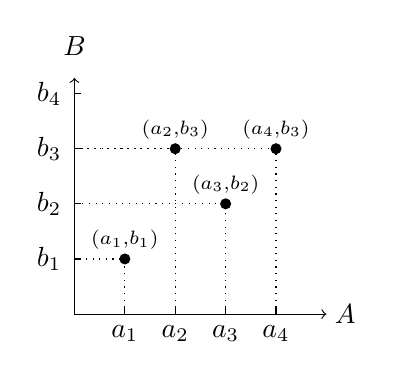
\begin{tikzpicture}[x=0.8cm]
  	\draw[->] (0,0) -- (4,0);
  	\draw[->] (0,0) -- (0,3.0);
  	\node at (4.3,0) {$A$};
  	\node at (0,3.4) {$B$};

      \draw (0.8,0) -- +(0,0.1) node [label=below:$a_1$]{};
      \draw (1.6,0) -- +(0,0.1) node [label=below:$a_2$]{};
      \draw (2.4,0) -- +(0,0.1) node [label=below:$a_3$]{};
      \draw (3.2,0) -- +(0,0.1) node [label=below:$a_4$]{};

      \draw (0,0.7) -- +(0.1,0) node [label=left:$b_1$]{};
      \draw (0,1.4) -- +(0.1,0) node [label=left:$b_2$]{};
      \draw (0,2.1) -- +(0.1,0) node [label=left:$b_3$]{};
      \draw (0,2.8) -- +(0.1,0) node [label=left:$b_4$]{};

  	\draw[dotted] (0.8,0) -- (0.8,0.7) -- (0,0.7);
  	\draw[dotted] (1.6,0) -- (1.6,2.1) -- (0,2.1);
  	\draw[dotted] (2.4,0) -- (2.4,1.4) -- (0,1.4);
  	\draw[dotted] (3.2,0) -- (3.2,2.1) -- (0,2.1);

  	\fill (0.8,0.7) circle (2pt) node[above] {$\scriptstyle (a_1,b_1)$};
  	\fill (1.6,2.1) circle (2pt) node[above] {$\scriptstyle (a_2,b_3)$};
  	\fill (2.4,1.4) circle (2pt) node[above] {$\scriptstyle (a_3,b_2)$};
  	\fill (3.2,2.1) circle (2pt) node[above] {$\scriptstyle (a_4,b_3)$};
  \end{tikzpicture}
\hfill
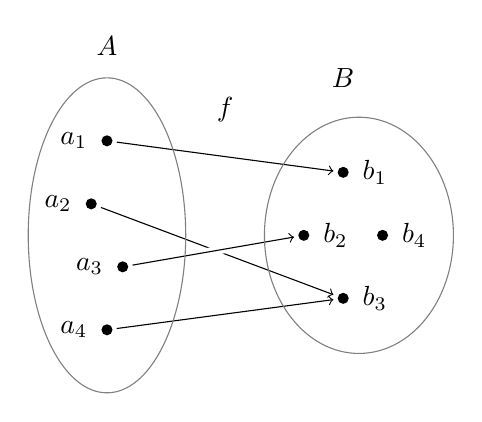
\begin{tikzpicture}[x=1cm,y=0.8cm]
\fill (1,4) circle (2pt) node (a1) [label=left:$a_1$]{};
\fill (0.8,3) circle (2pt) node (a2) [label=left:$a_2$]{};
\fill (1.2,2) circle (2pt) node (a3) [label=left:$a_3$]{};
\fill (1,1) circle (2pt) node (a4) [label=left:$a_4$]{};
\fill (4,3.5) circle (2pt) node (b1) [label=right:$b_1$] {};
\fill (3.5,2.5) circle (2pt) node (b2) [label=right:$b_2$] {};
\fill (4,1.5) circle (2pt) node (b3) [label=right:$b_3$] {};
\fill (4.5,2.5) circle (2pt) node (b4) [label=right:$b_4$] {};
\draw[->] (a1) edge (b1);
\draw[->] (a2) edge (b3);
\draw[line width=3pt,white] (a3) edge (b2);
\draw[->] (a3) edge (b2);
\draw[->] (a4) edge (b3);
\draw[draw=gray](1,2.5) ellipse (1cm and 2cm);
\draw[draw=gray](4.2,2.5) ellipse (1.2cm and 1.5cm);
\node at (1,5.5) {$A$};
\node at (4,5) {$B$};
\node at (2.5,4.5) {$f$};
\end{tikzpicture}
\hfill
\mbox{}
\caption[]{La funzione $f\colon A\to B$,
$f=\{a_1\mapsto b_1,$ $a_2 \mapsto b_3,$ $a_3 \mapsto b_2,$ $a_4 \mapsto b_3\}$
definita sull'insieme $A=\ENCLOSE{a_1, a_2, a_3, a_4}$
a valori nell'insieme $B=\ENCLOSE{b_1, b_2, b_3, b_4}$
rappresentata tramite grafico e
tramite diagrammi di Venn.}
\label{fig:funzione}
\end{figure}

L'insieme di partenza $A$ viene chiamato \emph{dominio}%
\mymargin{dominio}%
\index{dominio} 
della funzione $f\colon A\to B$,
mentre l'insieme di arrivo $B$ viene chiamato \emph{codominio}%
\mymargin{codominio}%
\index{codominio}.
La funzione $f$ rappresenta quindi un modo di assegnare in maniera univoca
ad ogni elemento del dominio un elemento del codominio.
Da un punto di vista informatico potremmo dire che $A$ è l'insieme
dei possibili \emph{input} e $B$ è l'insieme dei possibili \emph{output}
della funzione $f$.

Per come l'abbiamo definita, una funzione è dunque un insieme.
In generale le funzioni potrebbero essere definite in altri modi oppure 
potrebbero essere un concetto primitivo: dunque nei capitoli seguenti useremo le funzioni 
senza assumere che esse siano a loro volta degli insiemi.
Ad esempio invece di scrivere $(a,b)\in f$ scriveremo sempre $f(a)=b$ 
oppure $a\stackrel f \mapsto b$.
Sarà comunque molto importante
considerare l'insieme che rappresenta $f$ ma questo verrà chiamato
\emph{grafico}%
\mymargin{grafico}%
\index{grafico} di $f$, $G_f$ e potrà essere definito in questo modo:
\[
  G_f = \ENCLOSE{(x,y)\in A \times B\colon f(x)=y}.
\]
Nella nostra costruzione risulta effettivamente $G_f = f$ ma, come abbiamo detto,
in generale è opportuno distinguere la funzione dal suo grafico.
Uno degli argomenti principali di questo corso è lo studio 
del grafico delle funzioni reali, cioè le funzioni 
con dominio e codominio nell'insieme dei numeri reali.

\subsection{invertibilità}

Capita molto spesso che un fenomeno possa essere modellizzato matematicamente
tramite una funzione: si sa che ad un certo \emph{input} $a$ corrisponde
un \emph{output} $b=f(a)$. Molto spesso il problema da risolvere è
quello di determinare l'\emph{input} giusto $a$ per ottenere l'\emph{output}
voluto $b$. Questo problema corrisponde ad \emph{invertire} la funzione $f$:
dato $b\in B$ determinare $x\in A$ tale che $f(x) = b$.

Una funzione $f\colon A \to B$ si dice essere \emph{surgettiva}%
\mymargin{surgettiva}%
\index{surgettiva} (o \emph{suriettiva})
se per ogni $b\in B$ esiste almeno un $x\in A$ per cui $f(x)=b$. Questo
significa che il problema dell'inversione ha almeno una soluzione, qualunque
sia $b\in B$.
Una funzione $f\colon A \to B$ si dice essere \emph{iniettiva}%
\mymargin{iniettiva}%
\index{iniettiva}
se non esistono due punti distinti $a,a' \in A$, $a\neq a'$ tali
che $f(a) = f(a')$. Questo significa che il problema dell'inversione
$f(x)=b$ ha al più una soluzione (la soluzione, se esiste, è unica).
Una funzione $f\colon A \to B$ si dice essere \emph{bigettiva}%
\mymargin{bigettiva}%
\index{bigettiva}
(o \emph{biettiva})
\index{biettiva}%
\index{bigettiva}%
\index{funzione!bigettiva}%
\index{invertibile}%
\index{funzione!invertibile}%
\index{biettiva}%
o
\emph{invertibile}%
\mymargin{invertibile}%
\index{invertibile}%
\mynote{\textbf{Attenzione:} in alcuni testi (tra cui~\cite{Giusti}) si considerano
invertibili le funzioni iniettive, anche se non surgettive.}
se è sia iniettiva che surgettiva. Questo significa
che il problema dell'inversione $f(x)=b$ ha una unica soluzione $x\in A$
qualunque sia $b\in B$. In particolare, se $f$ è invertibile, per ogni $b\in B$ esiste
un unico $a\in A$ per cui $f(a)=b$.
Se $f$ è una funzione invertibile allora la relazione inversa $g$
cioè la relazione tale che $b\stackrel g \mapsto a$ quando $a \stackrel f \mapsto b$
risulta essere una funzione $g\colon B\to A$. 
Infatti $g$ è definita su tutto $B$ in quanto $f$ è surgettiva 
e $g$ è univoca in quanto $f$ è iniettiva.
Le proprietà caratteristiche della \emph{funzione inversa}%
\mymargin{funzione inversa}%
\index{funzione!inversa} $g$ sono:
\begin{equation}\label{eq:572098}
  \forall a\in A\colon g(f(a)) = a, \qquad
  \forall b\in B\colon f(g(b)) = b.
\end{equation}
La funzione $g$ inversa di $f$ viene usualmente denotata con il simbolo $f^{-1}$.

Se $f\colon A\to B$ è bigettiva diremo che $A$ 
e $B$ sono in \emph{corrispondenza biunivoca}%
\mymargin{corrispondenza biunivoca}%
\index{corrispondenza!biunivoca} tramite $f$.
In effetti $f$ è una corrispondenza \emph{univoca} da $A$ in $B$
(manda in modo univoco ogni punto di $A$ in un punto di $B$)
e $f^{-1}$ è una corrispondenza univoca da $B$ in $A$.

Introduciamo ora delle notazioni che sarà comodo utilizzare nel seguito.
Se $f\colon A \to B$ è una funzione e se $C\subset A$ definiamo
\[
  f(C) 
  = \ENCLOSE{f(a)\colon a \in C} 
  = \ENCLOSE{b\in B\colon \exists a\in C\colon b=f(a)}.
\]
L'insieme $f(C)\subset B$ si chiama \emph{immagine}%
\mymargin{insieme immagine}%
\index{immagine}
\index{immagine!insieme}%
di $C$ (tramite $f$) ed è formato
da tutti i punti che si ottengono applicando $f$ agli elementi di $C$.
L'immagine $f(A)$ dell'intero dominio $A$ si chiama immagine di $f$
e si denota a volte con il simbolo $\Im f$.
Si noti che $f$ è surgettiva se e solo se $f(A)=B$ (cioè se l'immagine coincide
col codominio).
Ad esempio la funzione definita in Figura~\ref{fig:funzione}
ha immagine $f(A) = \ENCLOSE{f(a_1),f(a_2),f(a_3),f(a_4)} 
 = \ENCLOSE{b_1, b_2, b_3}$.

Anche se $f\colon A \to B$ non fosse iniettiva,
per ogni $C\subset B$ possiamo definire
\[
  f^{-1}(C) = \ENCLOSE{a\in A\colon f(a) \in C}.
\]
L'insieme $f^{-1}(C)\subset A$ si chiama \emph{preimmagine}
o \emph{controimmagine}
\mymargin{preimmagine}%
\index{preimmagine}%
\index{preimmagine!insieme}%
\index{controimmagine!insieme}%
\index{insieme!controimmagine}%
di $C$ (tramite $f$)
ed è formato da tutti i punti di $A$ che applicando $f$ vanno in $C$.
Si noti che se $b\in B$ l'insieme $f^{-1}(\ENCLOSE{b})$ non è altro che
l'insieme delle soluzioni dell'equazione $f(x)=b$. Come abbiamo
già visto tale insieme contiene almeno un elemento se $f$ è suriettiva,
contiene al più un elemento se $f$ è iniettiva e contiene esattamente
un elemento $f^{-1}(\ENCLOSE{b}) = \ENCLOSE{f^{-1}(b)}$ se $f$ è bigettiva.
Ad esempio se $f$ è la funzione definita in figura~\ref{fig:funzione}
si ha $f^{-1}(\ENCLOSE{b_3,b_4}) = f^{-1}(\ENCLOSE{b_3}) = \ENCLOSE{a_2,a_4}$,
$f^{-1}(\ENCLOSE{b_4}) = \emptyset$.


La notazione $f(C)$ appena introdotta è formalmente ambigua in quanto
potrebbe non essere chiaro se $C$ è un elemento oppure un sottoinsieme
del dominio di $f$.
In pratica il contesto dovrebbe rendere chiaro cosa si intende.

Più in generale ci capiterà di estendere questo abuso di notazione non solo
alle funzioni, ma anche alle relazioni e alle operazioni.
Ad esempio se $A$ e $B$ sono insiemi di numeri ci capiterà di scrivere $A\le B$
per intendere che ogni elemento di $A$ è minore o uguale ad ogni elemento di $B$
oppure $A+B$ per intendere l'insieme di tutti i numeri che si ottengono sommando
ogni numero elemento di $A$ ad ogni numero elemento di $B$.

\begin{exercise}
  Sia $f\colon A \to B$ una funzione qualunque. 
  Si verifichi che se $C\subset A$ e $D\subset B$ si ha 
  \[
    f^{-1}(f(C))\supset C,
    \qquad 
    f(f^{-1}(D)) \subset D. 
  \]
  
  Che ipotesi possiamo fare su $f$ per avere l'uguaglianza
  $f(f^{-1}(C)) = C$?
  E per avere $f^{-1}(f(D)) = D$?
\end{exercise}

Si osservi che se $f\colon A \to B$ è una funzione e 
se $C\supset f(A)$ allora risulta anche $f\colon A \to C$ in quanto 
i valori di $f$ sono elementi di $C$. 
Dunque il \emph{codominio} di una 
funzione può essere esteso o ristretto con l'accortezza di mantenere 
tutti i valori dell'immagine. 
In particolare $f\colon A \to f(A)$ è certamente surgettiva.

Ad esempio vedremo che la funzione $\sin$ 
sarà definita con dominio l'insieme $\RR$ dei numeri reali 
ma può avere come codominio sia $\RR$ stesso
che solamente l'intervallo $[-1,1]$ dei numeri compresi 
tra $-1$ e $1$. 
Non ha quindi senso chiedersi se $\sin$ è suriettiva finché 
non dichiaro qual è il codominio considerato:
$\sin\colon \RR\to[-1,1]$ è suriettiva mentre 
$\sin\colon \RR\to\RR$ non lo è. 
Altri testi considerano il codominio parte della definizione 
della funzione e quindi considerano diverse due funzioni 
che hanno lo stesso grafico ma codominio diverso. 
E' una sottigliezza di poca rilevanza.

Per rendere iniettiva una funzione dobbiamo invece restringere il dominio.

\begin{definition}[restrizione]
  \label{def:restrizione}%
  Se $f\colon A\to B$ è una funzione e $C\subset A$, possiamo 
  \emph{restringere} il dominio di $f$ all'insieme $C$.
  \mynote{La notazione $f\llcorner C$ non è del tutto standard,
  probabilmente è più comune la notazione $f_{|C}$.}%
  Si ottiene una nuova funzione $f\llcorner C$ che coincide con $f$
  ma che è definita solo su $C$: $f\llcorner C\colon C\to B$:
  \[
  f\llcorner C(x) = f(x)\qquad 
  \forall x \in C.
  \]
\end{definition}


\subsection{funzione composta}
\index{composizione!di funzioni}%

Se $f\colon A\to B$ e $g\colon B\to C$ allora un punto $a\in A$ 
viene mandato tramite $f$ in un punto $b\in B$ e 
a sua volta il punto $b$ viene mandato da $g$ in un punto 
$c \in C$. 
La funzione che manda $a$ in $c$ viene chiamata 
\emph{funzione composta}%
\mymargin{funzione composta}%
\index{funzione!composta} si denota con $g\circ f$ 
e si può definire così:
\[
g\circ f \colon A \to C, \qquad 
(g\circ f)(x) = g(f(x)).  
\]

Se abbiamo tre funzioni 
$f\colon A\to B$, $g\colon B\to C$ e $h\colon C\to D$ 
allora è facile verificare che:
\[
   h \circ (g\circ f) = (h\circ g) \circ f
\]
in quanto per ogni $x\in A$ si ha
\[
(h \circ (g\circ f)) (x) =
h(g(f(x))) = (h\circ g)(f(x)) = ((h\circ g) \circ f) (x).  
\]
Significa che l'operatore di composizione $\circ$
soddisfa la proprietà associativa.

Se $f\colon A\to B$ è bigettiva allora 
per ogni $x\in A$ e per ogni $y\in B$ si ha,
grazie a~\eqref{eq:572098},
\[
  f^{-1} (f(x)) = x,
  \qquad f(f^{-1}(y)) = y.
\]
Significa che 
\[
  f^{-1}\circ f = \id_A, 
  \qquad
  f\circ f^{-1} = \id_B
\] 
dove $\id_X\colon X\to X$
è la funzione 
\emph{identità}%
\mymargin{identità}%
\index{identità} 
\index{funzione!identità}%
cioè la funzione 
che lascia fisso ogni punto di $X$:
\mymargin{$\id_X$}%
\index{$\id$}%
\[
\id_X(x) = x \qquad \text{per ogni $x\in X$}.
\]

\begin{theorem}
Se $f\colon A\to B$ e $g\colon B\to C$ sono entrambe invertibili
anche $g\circ f\colon A\to C$ è invertibile e si ha 
\begin{equation}\label{eq:inversa_composta}
  (g\circ f)^{-1} = f^{-1}\circ g^{-1}.
\end{equation}
\end{theorem}
\begin{proof}    
Per ogni $c\in C$ esiste un unico $b\in B$ tale che $g(b)=c$ 
ed un unico $a\in A$ tale che $f(a)=b$. 
Tale $a$ è l'unico punto per cui $g(f(a))=c$ e questo dimostra che 
$g\circ f$ è bigettiva. Inoltre $a=f^{-1}(b)$ e $b=g^{-1}(c)$ 
dunque $(g\circ f)^{-1}(c) = a = f^{-1}(g^{-1}(c))$ da cui si ottiene 
\eqref{eq:inversa_composta}.
\end{proof}

\begin{exercise}
  Si verifichi che la composizione di funzioni iniettive è iniettiva e la composizione 
  di funzione suriettive è suriettiva.
\end{exercise}

\subsection{cardinalità}

\begin{definition}[cardinalità]
  Diremo che due insiemi $A$ e $B$ hanno la stessa \emph{cardinalità}%
\mymargin{cardinalità}%
\index{cardinalità} 
  (oppure sono \emph{equipotenti}) 
  \index{equipotenza}%
  \index{insiemi!equipotenti}%
  \index{insieme!equipotente}%
  se esiste una funzione bigettiva $f\colon A \to B$.
  Scriveremo in tal caso:
  \[
    \# A = \# B.  
  \] 
  Se esiste una funzione iniettiva $f\colon A\to B$ significa che 
  $A$ ha la stessa cardinalità di un sottoinsieme di $B$ (in quanto $f\colon A \to f(A)$
  risulta essere bigettiva). Scriveremo in tal caso:
  \[
    \# A \le \#B.
  \]
\end{definition}

Intuitivamente se due insiemi hanno la stessa cardinalità 
significa che hanno lo stesso numero di elementi.
Ma la precedente definizione riesce a catturare tale concetto senza dover 
ricorrere al concetto di numero. 
Questo ha il vantaggio di rendere questa definizione applicabile 
a qualunque insieme, anche con \emph{infiniti} elementi.

Si osservi che non abbiamo dato una definizione di $\#A$ e quindi non stiamo 
definendo cos'è la cardinalità di un insieme ma stiamo soltanto definendo 
una relazione tra insiemi che 
denotiamo, impropriamente, utilizzando una uguaglianza: $\#A = \#B$.

E' ovvio che $\#A = \#A$ in quanto l'identità $\id_A$ è bigettiva.
E' anche chiaro che se $\#A = \#B$ e $\#B = \#C$ allora $\#A = \#C$ in quanto 
componendo tra loro due funzioni bigettive si ottiene ancora una funzione 
bigettiva. 
Infine se $\#A = \#B$ allora $\#A \le \#B$ (in quanto le funzioni bigettive 
sono iniettive) ed è chiaro che se $\#A \le \#B$ e $\#B \le \#C$ allora 
$\#A\le \#C$ (in quanto composizione di funzioni iniettive è iniettiva).

Possiamo definire il simbolo inverso $\#A \ge \#B$ 
come $\#B\le \#A$.
Se $B\neq \emptyset$ 
il seguente teorema ci dice che $\#A \ge \#B$ 
è equivalente a dire che 
esiste $f\colon A \to B$
surgettiva. 
%

\begin{theorem}\label{th:95444}
  Sia $B\neq \emptyset$.
  Esiste $f\colon A\to B$ surgettiva 
  se e solo se esiste $g\colon B\to A$ iniettiva.
\end{theorem}
% 
\begin{proof}
Da un lato se esiste $g\colon B\to A$ iniettiva, allora $g$ è una bigezione 
tra $B$ e $g(B)$. La funzione inversa $f\colon g(B) \to B$ 
\mynote{Questa funzione $f$ si chiama 
\emph{inversa sinistra}
\index{inversa!sinistra}%
di $g$ in quanto si ha $f(g(y))=y$ per ogni $y\in B$}
può essere estesa a tutto $A$ fissando un valore qualunque 
(questo si può fare se $B$ non è vuoto) nei punti di $A\setminus g(B)$
ottenendo quindi una funzione surgettiva da $A$ in $B$.
D'altro lato se esiste una funzione $f\colon A\to B$ surgettiva,
per ogni $b\in B$ l'insieme $f^{-1}(\ENCLOSE{b})$ non è mai 
vuoto e quindi è chiaro che debba esistere 
una funzione $g\colon B\to A$ tale che $g(b)$ è un qualunque elemento 
di tale insieme
\mynote{Questa funzione $g$ si chiama 
\emph{inversa destra} 
\index{inversa!destra}%
di $f$ 
in quanto $f(g(y))=y$ per ogni $y\in B$}
(qui si utilizza l'assioma~\ref{axiom:AC} discusso più sotto). 
Chiaramente $g$ è iniettiva.
\end{proof}

Nella dimostrazione del teorema precedente abbiamo utilizzato il seguente assioma 
della teoria degli insiemi che, sorprendentemente, non è conseguenza degli assiomi 
che abbiamo già introdotto finora.

\begin{axiom}[della scelta]%
  \label{axiom:AC}%
  \index{assioma!della scelta}%
  \index{scelta!assioma della}%
  \index{AC}%
  Sia $F\colon A \to \mathcal P(B)$
  una funzione tale che $F(a)\neq \emptyset$ 
  per ogni $a\in A$. Allora esiste una funzione
  $f\colon A \to B$ tale che $f(a)\in F(a)$
  per ogni $a\in A$.
\end{axiom}

L'assioma della scelta (denotato spesso con \emph{$AC$}%
\mymargin{$AC$}%
\index{AC}, \emph{axiom of choice})
è un assioma per certi versi controverso
e alcuni matematici preferiscono non utilizzarlo nelle loro dimostrazioni.
Il sistema formale che definisce la teoria degli insiemi senza 
introdurre l'assioma della scelta 
si chiama \emph{$ZF$}%
\mymargin{$ZF$}%
\index{ZF} (Zermelo-Fraenkel) mentre 
se si aggiunge l'assioma della scelta (choice) la teoria si chiama 
\emph{$ZFC$}%
\mymargin{$ZFC$}%
\index{ZFC}.

Grazie all'assioma della scelta è anche possibile dimostrare 
che dati due insiemi $A$ e $B$ le loro cardinalità
si possono confrontare: $\#A\le \#B$ oppure 
$\#B\le \#A$. 
La dimostrazione però diventa complicata e va oltre i nostri scopi.

Il seguente teorema dimostra invece la proprietà antisimmetrica 
della relazione tra cardinalità. 
E' probabilmente il primo vero teorema 
(con dimostrazione decisamente non banale) 
che andiamo a dimostrare.

\begin{theorem}[Cantor-Bernstein]%
  \label{th:cantor_bernstein}%
  \index{teorema!di Cantor-Bernstein}%
  \index{Cantor-Bernstein!teorema di}%
  Se $\#A \le \#B$ e $\#B \le \#A$ allora $\#A = \#B$.
\end{theorem}
%
\begin{figure}
  \centering
  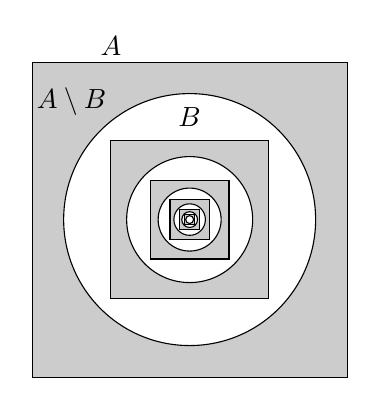
\begin{tikzpicture}
    \foreach \x in {1,0.5,0.25,0.25*0.5,0.25*0.25,0.25*0.25*0.5} {
      \path[draw,fill=black!20] (2*\x,2*\x)--(-2*\x,2*\x)--(-2*\x,-2*\x)--(2*\x,-2*\x)--cycle;
      \draw[fill=white] (0,0) circle (1.6*\x);
    };
    \node at (-1.0,2.2) {$A$};
    \node at (-1.5,1.5) {$A\setminus B$};
    \node at (0,1.3) {$B$};
%    \node at (-0.75,0.75) {$$};
  \end{tikzpicture}
  \caption{
  Nella dimostrazione del teorema di Cantor-Bernstein
  $A$ è rappresentato da un quadrato e $B$ da un cerchio contenuto
  in $A$. L'immagine di $A$ in $B$ è rappresentata da un quadrato contenuto
  in $B$ e così via. La parte ombreggiata è l'insieme $D$.
  }
  \label{fig:omotetia}
\end{figure}
%
\begin{proof}
Per ipotesi sappiamo che esiste
$g\colon B\to A$ iniettiva. 
Posto $B'=g(B)$ risulta che $g\colon B\to B'$ è bigettiva.
Ma allora dimostrare che esiste una bigezione tra $A$ e $B$ 
è equivalente a dimostrare che esiste una bigezione tra 
$A$ e $B'$. 
Dunque senza perdere di generalità, sostituendo $B'$ a $B$ 
possiamo supporre che sia $B\subset A$.

Essendo per ipotesi $\#A \le \#B$ esiste $f\colon A \to B$ iniettiva.
Intuitivamente l'idea è quella di definire l'insieme
\[
 D = (A\setminus B)  
 \cup f(A\setminus B) 
 \cup f(f(A\setminus B)) 
 \cup \dots
\]
e di definire la bigezione $\phi \colon A \to B$ 
utilizzando $f$ sull'insieme $D$ e lasciando fisso
il resto.

Per farlo in maniera rigorosa
consideriamo la famiglia di insiemi 
$\F = \{X \subset A \colon X \supset A \setminus B, f(X) \subset X\}$ 
e definiamo $D = \bigcap \F$.
Osserviamo che $A \in \F$ quindi $\F\neq \emptyset$.
Abbiamo in pratica definito $D$ come il più piccolo 
sottoinsieme di $A$ che viene mandato in se stesso da $f$.

E' facile verificare che $f(D) \subset D$ infatti dato $x\in D$ per ogni $X\in \F$ deve essere $x\in X$ ma allora $f(x) \in X$ (per come è definito $\F$), dunque $f(x) \in D$. 
In modo analogo si dimostra che $D\supset A\setminus B$ e dunque concludiamo che $D\in \F$.

Verifichiamo ora che $f(D)=D\cap B$. Da un lato se $x\in D$ allora
$f(x) \in f(D)\subset D$ e $f(x)\subset f(A)\subset B$ da cui $f(x) \in D\cap B$.
Dall'altro lato se $y\in D \cap B$ e non fosse $y \in f(D)$
allora potremmo considerare l'insieme $X=D\setminus\{y\}$
e osservare che $X\in \F$.
Infatti in primo luogo $X \supset A \setminus B$ in quanto $D$ ha questa proprietà e $y \in B$.
Inoltre dato qualunque $x \in X$ visto che $X\subset D$ allora
$f(x) \in f(D)$ e, per ipotesi,
$y\not \in f(D)$ dunque $f(x)\neq y$ da cui $f(x) \in X$.
Dunque $X\in \F$ ma allora dovrebbe essere $D\subset X$ mentre
per costruzione abbiamo $y\in D$ ma non in $X$.

% Avendo visto che $f(D)=D\cap B$ possiamo facilmente
% osservare che $f(A\setminus D) \subset A \setminus D$.
% Infatti $f(A\setminus D)\subset f(A)=B$ e quindi
% $f(A\setminus D)\cap D \subset D \cap B = f(D)$
% ma essendo $f$ iniettiva si deve avere
% $f(A\setminus D) \cap f(D)=\emptyset$.

Possiamo allora definire $\phi \colon A \to B$
\[
\phi(x) =
\begin{cases}
   f(x) & \text{se $x\in D$}, \\
   x & \text{altrimenti.}
\end{cases}
\]
Chiaramente $\phi$ è iniettiva in quanto $f$ è iniettiva e manda $D$ in $D$
e l'identità è iniettiva e manda $A\setminus D$ in $A\setminus D$.

Per dimostrare che $\phi$ è suriettiva consideriamo qualunque $y \in B$.
Se $y\not \in D$ allora $\phi(y)=y$.
Se invece $y\in D$ essendo $y\in D\cap B = f(D)$ esisterà $x\in D$ tale
che $\phi(x) = f(x) = y$.
\end{proof}

Possiamo ora determinare se un insieme $X$ è finito o infinito.
Gli insiemi infiniti sono quelli che possono essere messi in corrispondenza 
biunivoca con un loro sottoinsieme proprio: esiste $f\colon X\to X$ 
tale che $f$ è iniettiva ma non suriettiva. 
Invece se un insieme è finito togliendo anche un solo punto
se ne diminuisce la cardinalità: se $f\colon X\to X$ è iniettiva
allora è anche suriettiva.

\begin{definition}[infinito]
  \label{def:infinito}%
  Diremo che un insieme $X$ è \emph{finito}
  \index{insieme!finito}%
  \index{finito!insieme}%
  \index{Dedekind!finito}%
  (più precisamente: Dedekind-finito)
  se ogni funzione iniettiva $f\colon X\to X$ è anche suriettiva.
  \mymargin{insieme finito}%
\index{insieme finito}%

  Diremo che un insieme $X$ è \emph{infinito} 
  (più precisamente Dedekind-infinito)
  \index{insieme!infinito}%
  \index{infinito!insieme}%
  \index{Dedekind!infinito}%
  se non è finito ovvero
  se esiste $f\colon X\to X$ iniettiva ma non suriettiva.
  \mymargin{insieme infinito}%
\index{insieme infinito}%
\end{definition}

Con gli assiomi che abbiamo introdotto finora non è possibile dimostrare 
che esistono insiemi infiniti. 
Sarà quindi necessario un apposito assioma.

\begin{axiom}[infinito]
  \label{axiom:infinito}%
  Esiste un insieme infinito. 
\end{axiom}

Molto spesso l'assioma di infinito viene espresso dicendo che esiste 
l'insieme $\omega$ che ha come elementi tutti gli 
ordinali di Von Neumann finiti.
\index{Von Neumann!ordinali finiti}%
\index{ordinali finiti di Von Neumann}%
\mynote{
Se denotiamo con $P(\alpha)$ il predicato 
$(\emptyset\in \alpha \land \forall n\colon n\in \alpha) \implies n\cup\ENCLOSE{n}\in \alpha$
allora l'assioma che garantisce l'esistenza di $\omega$ si può 
scrivere nella forma:
  $\exists \omega\colon (P(\omega) \land \forall \alpha\colon P(\alpha)\implies \omega\subset \alpha)$
}

Nei capitoli~\ref{sec:cardinali_finiti} e \ref{sec:cardinali_infiniti}
vedremo ulteriori proprietà della cardinalità, ma prima 
dobbiamo familiarizzare con gli insiemi numerici.

\section{i numeri naturali}

I numeri naturali $0,1,2,\dots$ sono i numeri che utilizziamo per contare o per 
fare le iterazioni. C'è un primo numero naturale, che per noi sarà $0$, e poi
per ogni numero naturale $n$ ce n'è uno successivo che chiameremo $\sigma(n)$. 
Partendo da $0$ e passando al successivo si raggiungono tutti i numeri naturali.

In questa parte del capitolo introduciamo concetti basilari 
che sono stati introdotti a partire dalla scuola elementare 
e quindi dovrebbero essere familiari a chiunque. 
Le definizioni e le dimostrazioni delle prorietà di questi insiemi numerici 
risultano molto noiose da riprodurre e preferiamo 
quindi trattarle a parte nel capitolo~\ref{sec:costruzione_reali}.

\begin{theorem}[assiomi di Peano]
  \label{th:assiomi_peano}%
  \mynote{Giuseppe Peano (1858--1932) vedi note storiche a pag.~\pageref{nota:Peano}} 
    \label{def:naturali}%
  \index{numeri!naturali}%
  \index{$\NN$}%
  \index{Peano}%
  \index{assiomi!di Peano}%
  \index{insieme!induttivo}%
  \index{induttivo}%
Esistono un insieme $\NN$, 
un elemento $0\in \NN$ 
e una funzione $\sigma\colon \NN\to\NN$ tali che
\mynote{Il primo assioma di Peano dice che numeri diversi hanno 
numeri successivi diversi. Il secondo assioma ci dice che il primo 
numero naturale, per noi lo $0$, 
non è il successore di nessun'altro mentre ogni altro numero 
ne ha uno precedente. Il terzo assioma, il principio di induzione, 
ci dice che ogni numero naturale può essere raggiunto dallo $0$ 
facendo un numero finito di passaggi al successore.
}
\begin{enumerate}
  \item $\sigma$ è iniettiva;
  \item $\sigma(\NN) = \NN \setminus\ENCLOSE{0}$;
  \item se $A\subset \NN$ e 
  \begin{enumerate} 
    \item[(i)] $0\in A$ 
    \item[(ii)] $n\in A \implies \sigma(n)\in A$
  \end{enumerate}
  allora $A=\NN$.
\end{enumerate}
\end{theorem}
%
\begin{proof}
  \mynote{Se si assume l'assioma di infinito nella forma forte dell'esistenza 
  dell'insieme $\omega$ degli ordinali finiti di Von Neumann 
  si può semplicemente 
  prendere $\NN=\omega$, $0=\emptyset$, $\sigma(n) = n\cup \ENCLOSE{n}$.}
  Lo si dimostra grazie all'assioma~\ref{axiom:infinito} di infinito.
  Si veda il teorema~\ref{th:esistenza_naturali}.
\end{proof}

Si può dimostrare inoltre (si veda il teorema~\ref{th:unicitaN}) che le proprietà 
enunciate nel teorema precedente caratterizzano univocamente l'insieme 
$\NN$ dei numeri naturali. 

Dato $n\in \NN$ il numero $\sigma(n)$ si chiama il \emph{successore}%
\mymargin{successore}%
\index{successore} di $n$. 
Il numero $0\in \NN$ che per assioma non è il successore di nessun'altro 
numero naturale si chiama \emph{zero}%
\mymargin{zero}%
\index{zero}. 
Il successore di $0$ viene chiamato \emph{uno} e si definisce 
come $1=\sigma(0)$. 
Allora scriveremo $n+1$ al posto di $\sigma(n)$ per denotare 
il successore del numero $n$.
Per comodità diamo un nome amche alle altre \emph{cifre decimali}%
\mymargin{cifre decimali}%
\index{cifre!decimali} 
ovvero ai primi numeri naturali:
\begin{equation}\label{eq:cifre}
\begin{gathered}
% 1 \defeq \sigma(0),\quad  
 2 \defeq \sigma(1),\quad
 3 \defeq \sigma(2),\quad 
 4 \defeq \sigma(3),\quad
 5 \defeq \sigma(4),\\ 
 6 \defeq \sigma(5),\quad 
 7 \defeq \sigma(6),\quad 
 8 \defeq \sigma(7),\quad 
 9 \defeq \sigma(8).
\end{gathered}
\end{equation}
Dunque $\sigma$ è l'usuale operazione del contare:
 \[
 0 \stackrel\sigma\mapsto 1 \stackrel\sigma\mapsto 2 \stackrel\sigma\mapsto 
 3 \stackrel\sigma\mapsto 4 \stackrel\sigma\mapsto 5 \stackrel\sigma\mapsto 
 6 \stackrel\sigma\mapsto \dots  
 \]
Il primi due assiomi servono a garantire che in questo processo del \emph{contare}%
\mymargin{contare}%
\index{contare}
troviamo sempre numeri diversi (non si torna mai indietro) in quanto nessun numero 
può avere come successore $0$ o un numero già incontrato in precedenza (che 
se non è zero è il successore di un altro numero).

Il fatto che $\sigma\colon \NN\to \NN$ sia iniettiva ma non suriettiva 
significa che $\NN$ può essere messo in corrispondenza biunivoca con 
$\sigma(\NN)$ che è un sottoinsieme proprio di $\NN$.
Dunque $\NN$ è necessariamente un insieme infinito 
(definizione~\ref{def:infinito}).
In particolare $\#\NN = \#\enclose{\NN \setminus\ENCLOSE{0}}$.
Questa proprietà è per certi versi paradossale
(paradosso di Galileo, o paradosso dell'hotel Hilbert)
\index{paradosso!di Galileo}%
\index{paradosso!degli insiemi infiniti}%
\index{hotel Hilbert}%
\index{Hilbert!hotel}%
e caratterizza gli 
insiemi infiniti, nel senso di Dedekind.%
\mynote{Galileo Galilei (1564--1642) vedi note storiche a pag.~\pageref{nota:Galileo}}%

\subsection{principio di induzione}

L'ultimo degli assiomi di Peano 
ci dice che se un sottoinsieme dei numeri naturali contiene lo 
zero e contiene il successore di ogni suo elemento, allora contiene tutti i 
numeri naturali.
Serve a garantire che il processo del contare esaurisca tutti 
i numeri naturali, e che quindi non ci siano dei naturali \emph{irraggiungibili}
partendo da zero.
Questa proprietà viene usualmente utilizzata mediante il seguente.

\mynote{%
Formalmente dovremmo dire che $P$ è una funzione da $\NN$ in $\{V,F\}$
dove $V$,$F$ sono due valori distinti che interpretiamo come vero e falso.
Infatti il concetto di \emph{predicato} non è definito all'interno del 
sistema formale, ma è un concetto esterno.
Ma è ovvio che ad ogni predicato $P$ corrisponde 
una funzione $P\colon \NN\to \{V,F\}$ e viceversa.
}

\index{principio!di induzione}%
\index{induzione matematica}%
\begin{theorem}[principio di induzione]
  Sia $P(n)$ un predicato.
  Se 
  \begin{enumerate}
    \item vale $P(0)$
    \item $\forall n\in \NN\colon P(n)\implies P(n+1)$
  \end{enumerate} 
  allora $\forall n\in \NN\colon P(n)$.
\end{theorem}
%
\begin{proof}
  Consideriamo l'insieme $A=\{n\in \NN\colon P(n)\}$.
  Grazie alle ipotesi del teorema possiamo applicare la terza
  proprietà dei numeri naturali per dedurre che $A=\NN$.
  Dunque $P(n)$ è soddisfatta per ogni $n\in\NN$.
\end{proof}

Tramite il principio di induzione è anche possibile 
definire funzioni (o operazioni) per induzione.
Se ad esempio vogliamo definire una funzione $f\colon \NN\to X$
basterà dichiarare il valore di $f(0)$ e definire $f(n+1)$ 
(cioè $f(\sigma(n)))$ a partire da $f(n)$.
Il principio di induzione (o meglio il teorema~\ref{th:induzione})
garantisce che $f$ sia univocamente definita su tutto $\NN$.
Questo metodo per definire una funzione si chiama 
\emph{definizione ricorsiva} in quanto definisce 
il valore della funzione sul termine $n$-esimo rifacendosi
al valore assegnato sui termini precedenti.
In particolare è possibile definire
su $\NN$ le operazioni di addizione, 
moltiplicazione ed elevamento a potenza
tramite le seguenti definizioni ricorsive:
\index{addizione!su $\NN$}%
\index{moltiplicazione!su $\NN$}%
\index{elevamento a potenza!su $\NN$}%
\begin{gather*}
  \begin{cases}
    n + 0 = n,\\
    n + \sigma(m) = \sigma(n+m);
  \end{cases}
  \qquad
  \begin{cases}
    n \cdot 0 = 0,\\
    n \cdot (m+1) = n\cdot m + n;
  \end{cases}
  \qquad
  \begin{cases}
    n^0 = 1,\\
    n^{m+1} = n\cdot n^m.
  \end{cases}
\end{gather*}

\begin{example}\label{ex235}
  Dimostrare che $2+3=5$.
\end{example}  
%
\begin{proof}[Svolgimento]
Possiamo utilizzare 
la proprietà $n+\sigma(m) = \sigma(n+m)$ ponendo $n=2$ e $m=2$.
Si ottiene quindi $2+3 = 2+\sigma(2) = \sigma(2+2)$.
Per sapere quanto fa $2+2$ usiamo nuovamente la stessa proprietà 
ma stavolta con $m=1$. 
Si ottiene infatti $2+2=2+\sigma(1)=\sigma(2+1)$.
Infine $2+1=2+\sigma(0)=\sigma(2+0) = \sigma(2) = 3$, 
$2+2=\sigma(3)=4$ e quindi $2+3 = \sigma(4)=5$.
\end{proof}

Definiamo infine una relazione d'ordine su $\NN$ 
con l'idea che quando sommo tra loro due numeri naturali 
quello che ottengo è un numero \emph{più grande}:
\index{relazione!d'ordine su $\NN$}%
\[
   n\le m \iff \exists k\in \NN \colon n+k = m.
\]

Si può facilmente osservare che se esiste $k\in \NN$ tale che $n+k=m$
allora tale $k$ è unico. 
Dunque se $m\ge n$ si può definire la differenza $k=m-n$
come quell'unico $k$ tale che $n+k=m$.

In maniera analoga se esiste $k\in \NN$ tale che $m=k\cdot n$
diremo che $m$ è un \emph{multiplo} di $n$ 
\index{multiplo}%
ovvero che $n$ \emph{divide} $m$ (si può scrivere $n\vert m$).
Anche in questo caso $k$ se esiste è unico e si 
chiama \emph{quoziente} di $m$ diviso $n$, 
\index{quoziente}%
scriveremo: $k=\frac m n$.

\begin{theorem}[operazioni su $\NN$]
Le operazioni di addizione e moltiplicazione 
soddisfano le seguenti proprietà:
  \begin{enumerate}
    \item elemento neutro:
      $n + 0 = 0 + n = n$,
      $n\cdot 1 = 1\cdot n = n$;
    \item elemento assorbente:
      $n\cdot 0 = 0$;
    \item proprietà associativa: 
      $(n+m)+k = n+(m+k)$, $(n\cdot m)\cdot k = n \cdot (m\cdot k)$
    \item proprietà commutativa: 
      $n+m = m+n$, $n\cdot m = m\cdot n$;
    \item proprietà distributiva:
     $k\cdot (n+m) = k\cdot n + k\cdot m$;
    \item proprietà invariantiva:
     se $m+k = n+k$ allora $m=n$;
  \end{enumerate}
l'elevamento a potenza soddisfa le seguenti proprietà:
\begin{enumerate}
  \item $n^0 = 1$;
  \item $n^1 = n$;
  \item $n^{m+k} = n^m \cdot n^k$;
  \item $(n^m)^k = n^{m\cdot k}$;
  \item $(n\cdot m)^k = n^k \cdot m^k$;
\end{enumerate}
l'ordinamento soddisfa infine queste proprietà:
\begin{enumerate}
  \item $n\le n$ (proprietà riflessiva);
  \item se $n\le m$ e $m\le k$ allora $n\le k$ (proprietà transitiva);
  \item se $n\le m$ e $m\le n$ allora $n=m$ (proprietà antisimmetrica);
  \item o $n\le m$ oppure $m\le n$ (dicotomia);
  \item monotonia:
   se $m\le n$ allora 
   $m+k\le n+k$, $m\cdot k \le n\cdot k$,
   $k^m \le k^n$ e $m^k \le n^k$. 
\end{enumerate}
\end{theorem}
\begin{proof}
  Si vedano i teoremi~\ref{th:proprieta_addizione},
  \ref{th:proprieta_moltiplicazione},
  \ref{th:proprieta_potenza}, \ref{th:proprieta_ordine_N}
  e~\ref{th:monotonia_naturali}.
\end{proof}

Si osservi che abbiamo definito $n^0=1$ per ogni $n\in \NN$,
compreso $n=0$. 
Dunque abbiamo consapevolmente definito $0^0=1$:
questa definizione (controversa) risulterà essere utile.
Si noti invece che $0^n=0$ solo se $n\neq 0$.
Infatti qualunque numero moltiplicato per $0$ dà zero, 
quindi una moltiplicazione ripetuta dà zero 
se c'è almeno un fattore nullo. 
Ma nel prodotto $0^0$ ci sono $0$ fattori $0$ quindi non c'è in effetti nessuna 
moltiplicazione per $0$. 
E' dunque naturale che il risultato sia $1$, 
l'elemento neutro della moltiplicazione.

\begin{exercise}
  Dimostrare per induzione che per ogni $n\in \NN$, $n\ge 4$ si ha 
  \[  
    2^n \ge n^2.
  \]
  Ovvero, dimostrare che per ogni $n\in \NN$ si ha 
  \[
    2^{n+4} \ge (n+4)^2.  
  \]
\end{exercise}

\subsection{rappresentazione posizionale dei numeri naturali}

Per rappresentare in modo efficiente qualunque numero naturale utilizziamo la 
\emph{notazione posizionale decimale}%
\mymargin{notazione posizionale decimale}%
\index{notazione!posizionale decimale}.
Ricordiamo che le cifre decimali $0,1,2,\dots, 9$ sono state definite in~\eqref{eq:cifre}
a pag~\pageref{eq:cifre}.
Il numero rappresentato da una sequenza finita di cifre decimali può essere 
definito ricorsivamente: una sequenza di una sola cifra rappresenta il numero 
corrispondente alla cifra stessa, una sequenza di $n+1$ cifre rappresenta il 
numero rappresentato dalle prime $n$ cifre, moltiplicato per $9+1$ (cioè dieci),
e sommato alla ultima cifra. 
Ad esempio la sequenza di cifre $4701$ (leggi: quattromilasettecentouno)
è definita così:
\[ 
  4701 = ((4\cdot(9+1)+7)\cdot(9+1)+0)\cdot(9+1)+1.
\]
Osservando che $10 = 9+1$ si scriverà
\begin{align*}
  4701 
  & = ((4\cdot 10 + 7)\cdot 10 +0)\cdot 10 + 1 \\
  & = \mathbf 4\cdot 10^3 + \mathbf 7\cdot 10^2 + \mathbf 0\cdot 10^1 + \mathbf 1 \cdot 10^0. 
\end{align*}

\begin{table}
  \begin{center}
    \bgroup
    \def\tabcolsep{3pt}
    \begin{tabular}{>{\small}r|>{\small}r>{\small}r>{\small}r>{\small}r>{\small}r>{\small}r>{\small}r>{\small}r>{\small}r}
      $+$       & 1 & 2 & 3 & 4 & 5 & 6 & 7 & 8 & 9 \\ \hline
      1         & 2 & 3 & 4 & 5 & 6 & 7 & 8 & 9 & 10 \\
      2         & 3 & 4 & 5 & 6 & 7 & 8 & 9 & 10 & 11 \\
      3         & 4 & 5 & 6 & 7 & 8 & 9 & 10 & 11 & 12 \\
      4         & 5 & 6 & 7 & 8 & 9 & 10 & 11 & 12 & 13 \\
      5         & 6 & 7 & 8 & 9 & 10 & 11 & 12 & 13 & 14 \\
      6         & 7 & 8 & 9 & 10 & 11 & 12 & 13 & 14 & 15 \\
      7         & 8 & 9 & 10 & 11 & 12 & 13 & 14 & 15 & 16 \\
      8         & 9 & 10 & 11 & 12 & 13 & 14 & 15 & 16 & 17 \\
      9         & 10 & 11 & 12 & 13 & 14 & 15 & 16 & 17 & 18
      \end{tabular}
      \qquad
      \begin{tabular}{>{\small}r|r>{\small}r>{\small}r>{\small}r>{\small}r>{\small}r>{\small}r>{\small}r>{\small}r}
        $\cdot$       & 2 & 3 & 4 & 5 & 6 & 7 & 8 & 9 \\ \hline
        2         & 4 & 6 & 8 & 10 & 12 & 14 & 16 & 18 \\
        3         & 6 & 9 & 12 & 15 & 18 & 21 & 24 & 27 \\
        4         & 8 & 12 & 16 & 20 & 24 & 28 & 32 & 36 \\
        5         & 10 & 15 & 20 & 25 & 30 & 35 & 40 & 45 \\
        6         & 12 & 18 & 24 & 30 & 36 & 42 & 48 & 54 \\
        7         & 14 & 21 & 28 & 35 & 42 & 49 & 56 & 63 \\
        8         & 16 & 24 & 32 & 40 & 48 & 56 & 64 & 72 \\
        9         & 18 & 27 & 36 & 45 & 54 & 63 & 72 & 81
      \end{tabular}
      \egroup
    \end{center}
    \label{tab:tabelline}
\caption{Le \emph{tabelline} dell'addizione e della moltiplicazione.}
\end{table}

Procedendo come nell'esempio~\ref{ex235} si può costruire la \emph{tabellina}
della somma, dove sono riportate le somme di tutte le coppie di cifre decimali
(tabella~\ref{tab:tabelline}).
Sfruttando la definizione e la proprietà distributiva del prodotto non sarà difficile 
costruire anche la \emph{tabellina} del prodotto, dove sono riportati i prodotti delle 
coppie di cifre decimali. 
Ad esempio una volta dimostrato che $7\cdot 7 = 49$ si può procedere 
a dimostrare che $7\cdot 8 = 56$ come segue:
\[ 
  7\cdot 8 = 7\cdot (7+1) = 7\cdot 7 + 7 = 49+7 
  = 4\cdot 10 + 9 + 7 = 4\cdot 10 + 16 =
  4\cdot 10 + 10 + 6 = 5\cdot 10 + 6 = 56.
\]

Una volta imparate a memoria le \emph{tabelline} è possibile svolgere le operazioni di addizione 
e moltiplicazione su qualunque coppia di numeri naturali espressi in forma decimale. 
L'algoritmo è quello della somma e della moltiplicazione in colonna che abbiamo imparato alla 
scuola elementare. Si può capire la correttezza di questi algoritmi con un esempio.
Proviamo a dimostrare che $34\cdot 56 = 1904$:
\begin{align*}
\mathbf{34}\cdot \mathbf{56} 
  &= \mathbf{34}\cdot (\mathbf 5\cdot 10+ \mathbf 6) 
   = \mathbf{34}\cdot \mathbf 6 + (\mathbf{34}\cdot \mathbf 5) \cdot 10 \\
  &= (\mathbf 3\cdot 10 + \mathbf 4)\cdot \mathbf 6 + (\mathbf 3\cdot 10 + \mathbf 4)\cdot \mathbf 5 \cdot 10 \\
  &= \mathbf{18}\cdot 10 + \mathbf{24} + (\mathbf{15}\cdot 10 + \mathbf{20})\cdot 10 \\
  &= \mathbf{1}\cdot 10^2+(\mathbf 8+\mathbf 2)\cdot 10 + \mathbf 4 + (\mathbf 1\cdot 10^2 + (\mathbf 5+\mathbf 2)\cdot 10 + \mathbf 0)\cdot 10 \\
  &= (\mathbf 1+\mathbf 1)\cdot 10^2 +\mathbf 0\cdot 10 + \mathbf 4 + (\mathbf 1\cdot 10^2 + \mathbf 7\cdot 10 + \mathbf 0)\cdot 10 \\
  &= \mathbf 2\cdot 10^2 + \mathbf 0\cdot 10 + \mathbf 4 + \mathbf 1\cdot 10^3+\mathbf 7\cdot 10^2 + \mathbf 0 \cdot 10\\
  &= \mathbf 1\cdot 10^3 + \mathbf 9\cdot 10^2 + \mathbf 0\cdot 10 + \mathbf 4
  = \mathbf{1904}.
\end{align*}

\subsection{fattoriale e semi-fattoriale}

Definiamo il 
\emph{fattoriale}%
\mymargin{fattoriale}%
\index{fattoriale} 
\index{"!}%
\index{$n$"!}%
di un numero naturale $n$
denotato con $n!$ (leggi: $n$ fattoriale) 
tramite la seguente definizione ricorsiva
\[
  \begin{cases}
    0! = 1 \\
    (n+1)! = (n+1) \cdot n!
  \end{cases}
\]
in tal modo risulta che $n!$ è il prodotto dei primi $n$ numeri naturali positivi:
\[
  n! = 1 \cdot 2 \cdot 3 \cdots n.  
\]

\begin{exercise}
  \label{ex:6734098}%
  Utilizzando il principio di induzione
  si dimostri che per ogni $n\in \NN$:
  \[
    (n+1)! \ge 2^n, \qquad
    n^n \ge n!
  \]
\end{exercise}

\begin{table}
  \begin{center}
  \begin{tabular}{r|>{\small}r>{\small}r>{\small}r>{\small}r>{\small}r}
  $n$       & 0 & 1 & 2 & 3 & 4 \\
  \footnotesize $n+5$     & 5 & 6 & 7 & 8 & 9 \\ \hline
  $2^n$     & 1 & 2 & 4 & 8 & 16 \\
  \footnotesize $2^{5+n}$ & 32 & 64 & 128 & 256 & 512 \\
  \footnotesize $2^{10+n}$ & 1024 & 2048 & 4096 & 8192 & 16384 \\
  \footnotesize $2^{15+n}$ & 32768 & 65536 & 131072 & 262144 & 524288 \\
  \footnotesize $2^{20+n}$ & 1048576 & 2097152 & 4194304 & 8388608 & 16777216 \\  \hline
  $3^n$                    & 1 & 3 & 9 & 27 & 81 \\
  \footnotesize $3^{5+n}$  & 243 & 729 & 2187 & 6561 & 19683 \\  \hline
  $n!$      & 1 & 1 & 2 & 6 & 24 \\
  \footnotesize $(5+n)!$  & 120 & 720 & 5040 & 40320 & 362880 \\
  \footnotesize $(10+n)!$  & 3628800 & 39916800 & 479001600 & 6227020800 & 87178291200 \\ \hline
  \footnotesize $10^{3n}$  &  & K (chilo) & M (mega) & G (giga) & T (tera) \\ 
  \footnotesize $10^{3(n+5)}$  & P (peta) & E (exa) & Z (zetta) & Y (yotta) \\ \hline
  \footnotesize $2^{10n}$  &  & Ki (chibi) & Mi (mebi) & Gi (gibi) & Ti (tebi) \\
  \footnotesize $2^{10(n+5)}$ & Pi (pebi)& Ei (exbi) & Zi (zebi) & Yi (yobi)
  \end{tabular}
  \end{center}
  \caption{I primi valori (e nomi) di alcune delle sequenze che abbiamo definito.
  Sarà utile in particolare ricordare che  $2^{10}=1024$ 
  è molto vicino a $10^3=1000$: questo giustifica i nomi simili utilizzati
  per le potenze di $2^{10}$ e per le potenze di $10^3$.
  }
  \end{table}
  
  A volte sarà utile considerare anche i prodotti di solamente i numeri
  pari o i numeri dispari fino ad un certo numero $n$. Questo
  si chiama \emph{semi-fattoriale}%
\mymargin{semi-fattoriale}%
\index{semi-fattoriale} e si indica con $n!!$
  Lo possiamo definire separatamente sui numeri pari (cioè 
  i numeri che si possono scrivere nella forma $2n$ con $n\in \NN$)
  e i numeri dispari (che scriviamo nella forma $2n+1$):
  \index{"!"!}
  \index{$n$"!"!}
  \index{doppio fattoriale}%
  \index{fattoriale!doppio}%
  \index{fattoriale!semi-fattoriale}%
  \index{semi-fattoriale}%
  \begin{align*}
    (2n)!! &= 2 \cdot 4 \cdot 6 \cdots (2n) \\
    (2n+1)!! &= 1 \cdot 3 \cdot 5 \cdots (2n+1).
  \end{align*}
  
  \begin{remark}
  \label{rem:doppio_fattoriale}%
  Si osservi che risulta
  \[
    (2n)!! = (2\cdot 1) \cdot (2\cdot 2) \cdot (2\cdot 3) \cdots (2\cdot n)
          = 2^n \cdot n!
  \]
  mentre
  \[
    (2n+1)!! = \frac{(2n+1)!}{2n!!} = \frac{(2n+1)!}{2^n\cdot n!}.
  \]
  Queste formule permettono di esprimere il semi-fattoriale utilizzando
  il fattoriale intero e le potenze.
  \end{remark}
  
\begin{exercise}
  Si dia una definizione per induzione del semi-fattoriale
  (separatamente per i pari e per i dispari)
  e si dimostrino, per induzione, le formule nell'osservazione precedente.
\end{exercise}


\subsection{sequenze finite o ennuple}
\index{ennuple}%
\index{sequenza!finita}%

Abbiamo già visto che se $A$ è un insieme possiamo definire l'insieme 
delle coppie di elementi di $A$ con il prodotto cartesiano tra insiemi: 
$A\times A$. 
Cosa rappresenta un prodotto ripetuto?
Gli insiemi $(A\times A)\times A$ e $A\times(A\times A)$ non sono 
uguali, in quanto il primo è un insieme di coppie il cui primo elemento 
è a sua volta una coppia, il secondo insieme invece è un insieme di coppie 
il cui secondo elemento è una coppia:
\begin{gather*}
  (A\times A)\times A = \ENCLOSE{((a_0,a_1),a_2)\colon a_0,a_1,a_2\in A},
  \\
  A \times (A\times A) = \ENCLOSE{(a_0,(a_1,a_2))\colon a_0,a_1,a_2\in A}.
\end{gather*}
Questi insiemi sono molto simili tra loro e potrebbero essere identificati.
Un'altro insieme molto simile è l'insieme $A^{3}$.  
Usando la definizione di Von Neumann, $3 = \ENCLOSE{0,1,2}$, l'insieme 
$A^{3}$ rappresenta l'insieme di tutte le funzioni 
$\vec a\colon \ENCLOSE{0,1,2}\to A$.
La funzione $\vec a$ è univocamente determinata dal suo valore nei 
tre punti del dominio: $a_0 = \vec a(0)$, $a_1=\vec a(1)$, $a_2=\vec a(2)$
in quanto $\vec a = \ENCLOSE{0\mapsto a_0, 1\mapsto a_1, 2\mapsto a_2}$.
Possiamo quindi identificare $\vec a$ con la tripla (o vettore) di valori:
\[
  \vec a = (a_0, a_1, a_2), \qquad a_0,a_1,a_2 \in A.  
\]
I valori $a_0$, $a_1$ e $a_2$ vengono anche chiamate \emph{coordinate}
o \emph{componenti} del \emph{vettore} $\vec a$.
\mymargin{coordinate, componenti, vettore}%
\index{coordinate, componenti, vettore}%
\index{coordinate!vettore}%
\index{componenti!vettore}%
\index{vettore}%
In effetti l'insieme $A^{2}$ può essere identificato con $A\times A$, l'insieme 
$A^{3}$ sarà l'insieme delle triple di elementi di $A$ e in generale se $n\in\NN$ 
identifichiamo con $A^{n}$ l'insieme delle $n$-uple (leggi: ennuple) di elementi 
\index{ennuple}%
di $A$:%
\mynote{
  Stiamo qui identificando $n\in \NN$ con l'insieme $\ENCLOSE{0,1,\dots, n-1}$.}%
\[
   \vec a \in A^{n} \iff 
   \vec a = (a_0, a_1, \dots, a_{n-1}).  
\]

Storicamente ci siamo abituati a contare partendo da $1$ invece che da $0$.
Per questo motivo è usuale numerare gli elementi di una $n$-upla con gli indici 
che vanno da $1$ a $n$ invece che da $0$ a $n-1$.
Dunque se $\vec a \in A^{3}$ sarà usuale scrivere 
$\vec a = (a_1, a_2, a_3)$ invece che $\vec a = (a_0, a_1, a_2)$.

\subsection{somme e prodotti finiti}
\index{sommatoria}%
\index{produttoria}%

Introduciamo ora su $\NN$ il concetto di somma (e prodotto) iterato.
Quello che ora facciamo su $\NN$ vale allo stesso modo sugli insiemi 
numerici che andremo a definire più avanti, in particolare lo useremo 
molto sull'insieme $\RR$ dei numeri reali. 
In generale potremmo considerare un insieme $A$ su 
cui è defina una operazione associativa 
con elemento neutro. 

\begin{definition}[monoide]%
\label{def:monoide}%
Sia $A$ un insieme su cui è definita una operazione $*$.
Se l'operazione è associativa: $x*(y*z) = (x*y)*z$ 
ed ha elemento neutro $e\in A$ tale che $e*x = x*e = x$
diremo che $A$ è un \emph{monoide}.
Se inoltre l'operazione è commutativa, $x*y=y*x$ 
diremo che $A$ è un \emph{monoide commutativo} (o abeliano).

Quando per l'operazione $*$ viene utilizzato il simbolo di addizione $+$
diremo che il monoide è additivo. In tal caso l'elemento neutro 
si chiama \emph{zero} e si indica con $0$.
Se utilizziamo invece il simbolo di moltiplicazione $x\cdot y$
diremo che il monoide è moltiplicativo. In tal caso l'elemento 
neutro si chiama \emph{unità} e si indica usualmente con $1$.
\end{definition}

L'insieme $\NN$ è un monoide commutativo sia con l'operazione di addizione $+$ 
(monoide additivo) che con l'operazione di moltiplicazione 
$\cdot$ (monoide moltiplicativo).

In generale se $A$ è un monoide additivo 
(o moltiplicativo) possiamo fare somme (o prodotti) di un numero 
arbitrario (ma finito) di addendi (o fattori) di $A$.
Più precisamente se $\vec a \in A^n$ 
è una $n$-upla di elementi di $A$, 
vogliamo definirne la somma e il prodotto:
\mynote{In questo ambito è usuale numerare gli elementi della 
$n$-upla a partire dall'indice $1$ invece che dall'indice $0$.}
\begin{equation}\label{eq:6122112}
\sum_{k=1}^n a_k = a_1 + a_2 + \dots + a_n,
\qquad 
\prod_{k=1}^n a_k = a_1 \cdot a_2 \dots a_n.
\end{equation}
Formalmente bisogna dare una definizione per induzione. 
Basterà dire che la somma (o il prodotto)
di zero addendi (o fattori) vale l'elemento neutro 
dell'operazione cioè $0$ per la somma (e $1$ per il prodotto).
La somma di $n+1$ addendi (o $n+1$ fattori) è la somma dei primi $n$ 
a cui aggiungiamo l'ultimo addendo (o moltiplichiamo per l'ultimo fattore).
Formalmente:
\[
  \begin{cases}
    \displaystyle\sum_{k=1}^{0} a_k = 0, \\
    \displaystyle\sum_{k=1}^{n+1} a_k = \enclose{\sum_{k=1}^{n} a_k} + a_{n+1};
  \end{cases}  \qquad
  \begin{cases}
    \displaystyle\prod_{k=1}^{0} a_k = 1, \\
    \displaystyle\prod_{k=1}^{n+1} a_k = \enclose{\prod_{k=1}^{n} a_k} \cdot a_{n+1}.
  \end{cases}
\]
La variabile $k$ che si trova nelle formule~\eqref{eq:6122112} è \emph{muta}: 
al suo posto si può utilizzare qualunque altra variabile che non
compaia altrove.

E' naturalmente possibile anche fare una somma a partire da un indice 
diverso da $0$:
\[
  \sum_{k=m+1}^{m+n} a_k = \sum_{j=1}^{n} a_{m+j}.
\]
Dal punto di vista mnemonico abbiamo fatto 
un \emph{cambio di variabile} $k=m+j$:
per $j=1$ si trova $k=m+1$ e per $j=n$ si trova $k=m+n$.

Si osservi che risulta:
\[
  x^n = \prod_{k=1}^n x, \qquad 
  n! = \prod_{k=1}^n k.  
\]
in quanto le definizioni ricorsive di potenze e fattoriale
coincidono con le definizioni ricorsive del prodotto sul lato destro.

\begin{theorem}
In un monoide commutativo, si ha:
  \[
  \sum_{k=1}^n  \enclose{a_k + b_k} 
  = \sum_{k=1}^n a_k + \sum_{k=1}^n b_k.
  \]

Sia $f\colon A\to A$ una funzione \emph{additiva}
cioè $f(0) = 0$ e $f(x+y)=f(x)+f(y)$.
Allora 
  \[
    \sum_{k=1}^n  f(a_k) = f\enclose{\sum_{k=1}^n a_k}.
  \]

Infine risulta 
  \[
  \sum_{k=1}^{m+n} a_k = \sum_{k=1}^m a_k + \sum_{k=1}^n a_{k+m}
  \]
ovvero 
  \[
  \sum_{k=1}^{m+n} a_k = \sum_{k=1}^m a_k + \sum_{k=m+1}^{m+n} a_k.  
  \]
\end{theorem}
\begin{proof}
  Le dimostrazioni possono essere svolte 
  per induzione.
\end{proof}

\begin{exercise}
  \label{ex:somma_lineare}%
  Dimostrare che 
  \[
    \sum_{k=1}^n k = \frac{n\cdot (n+1)}{2}, \qquad
    \sum_{k=1}^n k^2 = \frac{n\cdot (n+1)\cdot (2n+1)}{6}.
  \]
\end{exercise}
Il risultato della prima somma può essere ricordato nel modo seguente:
la media di una progressione aritmetica $\frac{1+2+ \dots + n}{n}$ 
è uguale alla media tra il primo 
e l'ultimo termine della progressione: $\frac{1+n}{2}$.
\begin{proof}[Svolgimento]

Una volta identificata la formula la possiamo dimostrare per induzione.
Per $n=0$ la somma è pari a $0$ per definizione.
Se la formula è vera per un certo $n$, si ha 
\[
  \sum_{k=1}^{n+1} k = \enclose{\sum_{k=1}^n k} + (n+1)
   = \frac{n\cdot(n+1)}{2} + (n+1) 
   = \frac{(n+2)(n+1)}{2}
\]
che è quanto volevamo dimostrare.

La formula per la somma dei quadrati si può dimostrare facilmente per 
induzione (lo si faccia per esercizio) se già conosciamo la formula da 
dimostrare.

Un metodo per trovare la formula è quello di osservare che la differenza 
di due termini cubici consecutivi risulta essere quadratico:
\[
(k+1)^3 - k^3 = 3 k^2 + 3k + 1.  
\]
Sommando ambo i lati della precedente equazione si ottiene:
\begin{equation}\label{eq:309838}
\sum_{k=1}^n (k+1)^3 - \sum_{k=1}^n k^3 
= 3\sum_{k=1}^n k^2+3\sum_{k=1}^n k+\sum_{k=1}^n 1.
\end{equation}
Al lato destro compare la somma di cui vogliamo calcolare il valore 
(moltiplicata per $3$)
insieme ad altre due somme di cui sappiamo già il valore. 
Basterà allora determinare il valore del lato sinistro dove 
osserviamo che i termini delle due somme si cancellano 
a vicenda,
\mynote{%
si chiama \emph{somma telescopica}
\index{somma!telescopica}%
\index{telescopico}%
in quanto i termini delle due sommatorie si chiudono uno nell'altro 
come i tubi di un cannocchiale.} %
tranne l'ultimo della prima somma 
e il primo della seconda: 
\[
  \sum_{k=1}^n(k+1)^3 - \sum_{k=1}^n k^3 = (n+1)^3 - 1^3.
\]
Moltiplichiamo per $2$ l'equazione~\eqref{eq:309838},
mettiamo in evidenza la somma dei quadrati e 
utilizzando la formula $2\sum_{k=1}^n k = n(n+1)$
per ottenere:
\begin{align*}
  6 \sum_{k=1}^n k^2 
  &=  2(n+1)^3 - 3 n(n+1) - 2n - 2
  = (n+1) \cdot \Enclose{2(n+1)^2 - 3n} - 2(n+1)\\
  &= (n+1)\cdot \Enclose{2n^2+4n+2 -3n - 2}
   = (n+1)\cdot \Enclose{2n^2+n} 
   = n \cdot (n+1)(2n+1)
\end{align*}
che è quanto volevamo dimostrare.
\end{proof}

\begin{exercise}
  Si trovi una formula per esprimere
  \[
  \sum_{k=1}^n k^3.
  \]
\end{exercise}

\begin{exercise}
Si noti che se prendiamo una progressione geometrica 
(potenze successive con la stessa base) 
ad esempio:
\[
  x = 3^3 + 3^4 + 3^5 + 3^6
\]
ogni addendo è uguale al precedente moltiplicato per $3$.
Dunque se moltiplichiamo per la base l'intera somma
\[
  3x = 3^4 + 3^5 + 3^6 + 3^7
\]
si ottiene la somma iniziale con un termine in più alla fine 
e un termine in meno all'inizio. 
\mynote{Anche questa è una somma \emph{telescopica}}
Facendo la differenza tutti i termini si cancellano tranne 
il primo e l'ultimo
\[
 3x - x = 3^7 - 3^3  
\]
e possiamo ricavare $x$.

Si formalizzi il ragionamento precedente per dimostrare che 
fissato $a\neq 1$ si ha per ogni naturale $n$:
  \[
    \sum_{k=0}^n a^k = \frac{a^{n+1}-1}{a-1}.
  \] 
\end{exercise}

Denotiamo con $\Enclose{n} = \ENCLOSE{0,1,2, \dots, n-1}$.
Se $\sigma\colon \Enclose{n} \to \Enclose{n}$
è bigettiva (una tale funzione si chiama \emph{permutazione}%
\mymargin{permutazione}%
\index{permutazione})
allora si può fare il cambio di variabile $k=g(j)$:
\[
    \sum_{k=0}^{n-1} a_k = \sum_{j=0}^{n-1} a_{\sigma(j)}.
\]
Questa uguaglianza può essere dimostrata facilmente nel caso 
in cui $\sigma$ scambi due soli indici lasciando fissi tutti gli altri 
(trasposizione) e poi può essere estesa a tutte le permutazioni
osservando che ogni permutazione si può scrivere come composizione 
di trasposizioni.

Questa proprietà è sostanzialmente la proprietà commutativa della somma 
estesa ad un numero qualunque di addendi.
Grazie a questa proprietà possiamo definire la somma di una funzione 
definita su qualunque insieme finito. 
Se $f\colon X \to M$
dove $M$ è un monoide, 
e $\sigma\colon \Enclose{n} \to X$ è una bigezione (dunque $\#X = n$)
allora si può definire 
\[
  \sum_{x\in X} f(x) = \sum_{j=0}^{n-1} f(\sigma(j))  
\]
in quanto la somma sul lato destro non dipende dalla bigezione $\sigma$ che 
abbiamo scelto.

\section{i numeri reali}

Intuitivamente si può ottenere l'insieme $\RR$ dei numeri reali
a partire da una retta geometrica 
con lo stesso procedimento con cui si costruisce un righello.
Iniziamo col segnare
sulla retta un punto di riferimento che chiamiamo $0$, 
dopodiché osserviamo che
il punto $0$ (come ogni altro punto) divide la retta in due parti. In modo arbitrario
chiamiamo positivi i punti che si trovano da una parte e negativi i punti che
si trovano dall'altra parte. Sulla semiretta dei numeri positivi scegliamo, arbitrariamente,
un punto $1$. Il segmento compreso tra i punti $0$ e $1$ sarà la nostra unità di
misura.
L'addizione potrebbe essere definita utilizzando i movimenti rigidi.
Traslando il punto $1$ di una unità alla volta si ottengono, per iterazione, tutti i numeri naturali.
Traslando all'indietro si ottengono i numeri interi negativi. 
Assumendo che tra due punti qualunque esistano sempre punti intermedi (divisibilità) e
assumendo che suddividendo la retta in due parti esista sempre un punto di 
suddivisione (continuità) mostreremo come si può suddividere 
ogni segmento in $n$ parti uguali per ogni numero naturale $n$. 
In tal modo potremo ritrovare i numeri razionali e la moltiplicazione per un numero razionale.
Con una estensione crescente riusciremo quindi a definire la moltiplicazione 
tra numeri reali. 
Osserveremo poi che la struttura moltiplicativa dei numeri reali positivi soddisfa 
gli stessi assiomi della struttura additiva dei reali e che quindi la costruzione fatta 
per costruire la moltiplicazione si potrà ripetere identica per costruire l'elevamento a potenza.

\subsection{gruppi ordinati}

L'insieme $\RR$ dei numeri reali si caratterizza 
con l'essere un \emph{gruppo totalmente ordinato denso e continuo}
in base alle seguenti definizioni.

\begin{definition}[relazione d'ordine]
  \label{def:ordine}%
  Una relazione
  $\le$ su un insieme $R$ viene detta
  \emph{relazione d'ordine}%
\mymargin{relazione d'ordine}%
\index{relazione!d'ordine}
  se soddisfa le seguenti proprietà (per ogni $x,y,z\in R$):
  \begin{enumerate}
    \item[1.] riflessiva: $x\le x$;
    \item[2.] antisimmetrica: $x\le y \land y\le x \implies x=y$;
    \item[3.] transitiva: $x\le y \land y\le z \implies x\le z$.
  \end{enumerate}
  Si dice inoltre che la relazione d'ordine $\le$
  è una relazione d'\emph{ordine totale}
\mymargin{ordine totale}%
  (o \emph{lineare}) 
  \index{ordinamento!totale}%
  \index{ordinamento!lineare}%
  \index{totale!ordine}%
  \index{lineare!ordine}%
  e si dice che $R$ è \emph{totalmente ordinato} se vale
  \index{totalmente ordinato}%
  \begin{enumerate}
    \item[4.] dicotomia: $x\le y \lor y\le x$.
  \end{enumerate}
\end{definition}

In generale, se $\le$ è una relazione d'ordine su $R$ si definisce la 
relazione inversa $\ge$ ponendo $x\ge y$ quando $y\le x$.
La proprietà riflessiva identifica gli ordinamenti \emph{larghi}.
Si definisce il corrispondente ordinamento stretto $<$
ponendo $x < y$ quando $x\le y \land x\neq y$
e la relazione inversa $>$ ponendo $x>y$ quando $y<x$.

\begin{definition}[funzioni monotòne]
  \label{def:monotonia}%
  Siano $R$ e $S$ insiemi ordinati 
  e sia $f\colon R\to S$.
  Diremo che $f$ è:
  \begin{enumerate}
    \item \emph{crescente} quando mantiene l'ordinamento: 
    per ogni $x,y\in R$ se $x\le y$ allora $f(x) \le f(y)$
    \item \emph{decrescente} quando inverte l'ordinamento: 
    per ogni $x,y\in R$ se $x\le y$ allora $f(y) \le f(x)$
    \item \emph{strettamente crescente} quando mantiene l'ordinamento stretto: 
    per ogni $x,y\in R$ se $x < y$ allora $f(x) < f(y)$
    \item \emph{strettamente decrescente} quando inverte l'ordinamento stretto: 
    per ogni $x,y\in R$ se $x < y$ allora $f(y) > f(x)$
    \item \emph{monotòna} se è crescente o decrescente
    \item \emph{strettamente monotòna} se è strettamente crescente 
    o strettamente decrescente
  \end{enumerate}
\end{definition}

\begin{definition}[ordinamento continuo]
  \label{def:ordinamento_continuo}%
  Un ordinamento $\le$ su un insieme $R$ si dice essere
  \emph{continuo}%
\mymargin{ordinamento continuo}%
\index{continuo}
  \index{continuità!ordinamento}%
  \index{ordine!continuo}%
  (o \emph{Dedekind-completo})
  \index{Dedekind-completo}%
  \index{completo!Dedekind}%
  se dati comunque $A,B$ sottoinsiemi non vuoti di $R$
    tali che per ogni $a\in A$ e per ogni $b\in B$ risulta $a\le b$
    (concisamente scriveremo $A\le B$ e diremo che $A$ e $B$ sono 
    \emph{separati})
    allora esiste $c\in R$ tale che per ogni $a\in A$ e ogni $b\in B$ 
    si ha $a\le c \le b$ (concisamente scriveremo $A\le c \le B$
    e diremo che $c$ è un elemento di separazione tra $A$ e $B$).
\end{definition}

A parole la precedente definizione si esprime dicendo che un insieme ordinato
è \emph{continuo} se ogni coppia di sottoinsiemi separati 
ammette un elemento di separazione.
In molti testi questa condizione viene chiamata \emph{completezza}
o, più precisamente, \emph{completezza di Dedekind}.
\index{completezza!di Dedekind}%
\index{Dedekind!completo}%

\begin{definition}[ordinamento denso]
  \label{def:ordinamento_denso}%
  Un ordinamento si dice essere
  \emph{denso}%
\mymargin{ordinamento denso}%
\index{denso} o \emph{divisibile} 
  se tra due punti distinti esiste sempre un punto intermedio:
  \index{denso!sottoinsieme}%
  \index{denso!ordinamento}%
  \index{sottoinsieme!denso}%
  \index{ordinamento!denso}%
  \mynote{Più in generale se $R$ è un insieme totalmente 
  ordinato e $A\subset R$ si dice che $A$ è denso in $R$ 
  se dati comunque $x,y\in R$ con $x<y$ esiste $c\in A$ tale che 
  $x<c<y$.}
  \[
   x < y \implies \exists c \colon x < c < y.
  \]
\end{definition}

\begin{definition}[gruppo]
  \label{def:gruppo}%
  Un insieme $R$ su cui è definita una \emph{operazione} $*$ 
%  \mynote{%
%  una operazione $*$ su $R$ è una funzione $*\colon R\times R \to R$ 
%  che si indica utilizzando la notazione \emph{infissa}: $x*y = *(x,y)$.}
%% già detto
  si dice essere un \emph{gruppo}%
\mymargin{gruppo}%
\index{gruppo} se l'operazione
  ha le seguenti proprietà:
  \begin{enumerate}
    \item associativa: $\forall x,y,z\in R\colon (x*y)*z = x*(y*z)$;
    \index{proprietà!associativa}%
    \index{associatività}%
    \item esistenza elemento neutro: 
    \index{elemento!neutro}%
    \index{neutro}%
    $\exists e\in R\colon \forall x\in R \colon e*x=x*e = x$;
    \item esistenza inverso: 
    \index{elemento!inverso}%
    \index{inverso}%
    $\forall x\in R\colon \exists y\in R\colon x*y=y*x=e$.
  \end{enumerate}
  Inoltre il gruppo si dice essere \emph{abeliano}%
\mymargin{gruppo abeliano}%
\index{abeliano} o \emph{commutativo}
  se vale la proprietà:
  \begin{enumerate}
    \item[4.] commutativa: $\forall x,y\in R\colon x*y = y*x$.
    \index{proprietà!commutativa}%
    \index{commutatività}% 
  \end{enumerate}
  
  Quando l'operazione viene denotata con il simbolo $+$ (addizione)
  diremo che il gruppo è additivo, denoteremo con $0$ 
  \index{zero}%
  (zero) l'elemento neutro e l'inverso di $x$ verrà chiamato \emph{opposto}
  e si denota con $-x$.
  \index{opposto}%
  Se invece si usa il simbolo $\cdot$ (moltiplicazione)
  diremo che il gruppo è moltiplicativo, l'elemento neutro potrà 
  essere denotato con il simbolo $1$ (uno o unità) e 
  \index{uno}\index{unità}%
  l'inverso di $x$ potrà essere chiamato \emph{reciproco}
  e si denota usualmente con $x^{-1}$ o $\frac 1 x$.
  \index{reciproco}%
  \end{definition}
  
  L'elemento neutro di un gruppo è unico. 
  Se infatti $x$ e $y$ fossero due elementi neutri 
  si avrebbe $x = x*y = y$. 
  Anche l'inverso è unico: infatti se $y$ e $z$ fossero 
  due inversi di $x$ si avrebbe $y = y * x * z = z$.
  
  \begin{definition}[gruppo ordinato]
    \label{def:gruppo_ordinato}%
    Diremo che $R$ è un \emph{gruppo ordinato}%
\mymargin{gruppo ordinato}%
\index{gruppo!ordinato} se $R$ è un gruppo
    (con operazione $*$ ed elemento neutro $e$),
    se è anche un insieme ordinato (con relazione $\le$)
    e se vale la proprietà:
    \begin{enumerate}
      \item[1.] monotonia: se $x\le y$ allora per ogni $z$ si ha:
       \[
       x*z \le y*z \qquad\text{e}\qquad z*x \le z*y.
       \] 
    \end{enumerate}
  \end{definition}

Su un gruppo additivo si può definire la moltiplicazione $n\cdot x$ per un numero 
naturale $n\in\NN$ come addizione ripetuta:
ad esempio $3\cdot x = x + x + x$.
Questo è garantito dal seguente.
%
\begin{theorem}[addizione ripetuta]
  \label{th:addizione_ripetuta}%
Sia $R$ un gruppo additivo. 
Esiste una unica operazione, $n \cdot x$ definita per $n\in \NN$ 
e $x\in R$ tale che
\[
\begin{cases}
  0\cdot x  = 0 \\
  (n+1) \cdot x = n\cdot x + x.
\end{cases}  
\]
Inoltre risulta:
\begin{enumerate}
  \item[1.] $1\cdot x = x$, $n\cdot 0 = 0$;
  \item[2.] $(n+m)\cdot x = n\cdot x + m\cdot x$; 
  \item[3.] $(n\cdot m)\cdot x = n\cdot (m\cdot x)$;
  \item[4.] $-(n\cdot x) = n\cdot(-x)$;
  \item[5.] se $n\cdot x = 0$ allora o $n=0$ o $x=0$;
\end{enumerate}
se il gruppo è abeliano si ha anche:
\begin{enumerate}
\item[6.] $n\cdot(x+y) = n\cdot x + n\cdot y$.
\end{enumerate}
e se il gruppo è totalmente ordinato si ha:
\begin{enumerate}
  \item[7.] se $x \le y$ allora $n\cdot x \le n\cdot y$;
  \item[8.] se $x < y$ e $n \neq 0$ allora $n\cdot x < n\cdot y$;
  \item[9.] se $x\ge 0$ e $n\ge m$ allora $n\cdot x\ge m\cdot x$;
\end{enumerate}
\end{theorem}
%
\begin{proof}
La dimostrazione si porta a termine facilmente dimostrando tutte le proprietà 
per induzione.
E' la stessa costruzione che abbiamo fatto per definire 
la moltiplicazione su $\NN$.
\end{proof}

\begin{theorem}[proprietà archimedea]
  \label{th:archimede}%
  \mymark{**}%
  \mymargin{proprietà archimedea}%
  \index{proprietà!archimedea}%
  \mynote{Questo teorema ci dice che il gruppo $R$ 
  non contiene né elementi \emph{infiniti} (cioè più grandi di qualunque 
  multiplo di un numero positivo $x$) 
  né elementi \emph{infinitesimi} (cioè più piccoli 
  di qualunque frazione $\frac{x}{n}$ con $x>0$ e $n\in \NN$).
  Dunque le quantità infinitesime
  utilizzate da Newton e Leibniz per definire derivate e 
  integrali, non sono giustificabili all'interno 
  di un gruppo totalmente ordinato denso e continuo.
  E' però possibile definire un gruppo totalmente ordinato 
  denso ma non continuo in cui esistono quantità infinite e infinitesime:
  è quello che viene fatto nella \emph{analisi non-standard}.
  \index{analisi non standard}%
  }
    Sia $R$ un gruppo totalmente ordinato, denso e continuo.
  Allora per ogni $x,y\in R$, $x>0$, $y>0$ 
  esiste $n\in \NN$ tale che $n\cdot x > y$.
\end{theorem}
%
\begin{proof}
\mymark{*}%
Fissato $x>0$ consideriamo gli insiemi:
\[
A = \NN\cdot x = \ENCLOSE{n\cdot x\colon n\in \NN},
B = \ENCLOSE{b\in R\colon \forall n\in\NN\colon n \cdot x \le b }.
\]
Per definizione $A\le B$ e $A$ è diverso dal vuoto.
Se per assurdo il teorema fosse falso, si avrebbe $y\in B$ 
e quindi anche $B$ sarebbe non vuoto.
Dunque per la continuità dell'ordinamento dovrebbe esistere 
un elemento di separazione $s\in R$ tale che $A\le s\le B$.
Visto che $s-x<s$ e $s\le B$,
sappiamo che $s-x \not \in B$.
Dunque esiste $n\in \NN$ tale che $n\cdot x > s-x$
ma allora $(n+1)\cdot x > s-x+x=s$. 
Ma questo è assurdo perché $(n+1)\cdot x\in A$ e $s\ge A$.
%
%%% dimostrazione col SUP
%  Fissati $x,y\in R$, $x,y>0$ consideriamo l'insieme 
%  \[
%     A = \NN \cdot y = \ENCLOSE{n\cdot y\colon n\in \NN}.
%  \]
%  Basta dimostrare che $A$ non è superiormente limitato perché 
%  in tal caso dato $x\in \RR$ esisterebbe $n\in \NN$ per cui $n\cdot y> x$.
%
%  Chiaramente $A$ non è vuoto in quanto $0\in A$ dunque se $A$ 
%  per assurdo fosse superiormente limitato esisterebbe 
%  $m=\sup A$, $m\in R$. 
%  Siccome $m$ è il minimo dei maggioranti di $A$
%  e $m-y$ è più piccolo di $m$, allora $m-y$ non è un maggiorante. 
%  Dunque deve esistere $n\in \NN$ tale che $ny>m-y$.
%  Ma allora $(n+1)y = ny + y > m$ ed essendo $n+1\in \NN$ troviamo che $m$
%  non poteva essere un maggiorante di $A$: assurdo.
\end{proof}

Se $n\cdot x = y$ e $n\neq 0$ scriveremo $x=\frac y n$. 
Affinché questa definizione sia univoca bisogna però verificare che 
se $n\cdot x = n\cdot x'$ allora $x=x'$.
Infatti si ha 
\[
  0 = n\cdot x - n\cdot x' = n\cdot (x-x')
\]
e se $n\neq 0$ si conclude $x-x'=0$ ovvero $x=x'$.

Il seguente teorema ci permette di dimostrare che la divisione per $n\neq 0$ 
si può sempre fare.
Si faccia presente che se interpretiamo questo teorema su un 
gruppo moltiplicativo, invece che additivo, il risultato
appare meno banale perché 
stiamo dimostrando l'esistenza della radice $n$-esima.

\begin{theorem}[divisibilità]
\label{th:divisibile}%
Se $R$ è un gruppo additivo totalmente ordinato, denso e continuo
allora per ogni $y\in R$, e per ogni $n\in \NN$, $n\neq 0$ 
esiste $x\in R$ tale che $n\cdot x = y$.
\end{theorem}
%
Per dimostrare il teorema ci servirà il seguente.
%
\begin{lemma}[esistenza di numeri piccoli]
  \label{lm:numeri_piccoli}%
Sia $R$ un gruppo additivo totalmente ordinato e denso.
Per ogni $y\in R$, $y>0$ ed ogni $n\in \NN$ esiste $x\in R$, 
$x>0$ tale che $nx\le y$.
\end{lemma}
%
\begin{proof}
Vogliamo innanzitutto dimostrare che 
\begin{equation}\label{eq:41095633}
  \forall y>0 \colon \exists x>0 \colon x+x \le y.
\end{equation}
Per la proprietà di densità sappiamo che esiste $z$ tale che 
$0<z<y$. 
Prendiamo $w=y-z$. Se $w\le z$ allora $w+w\le w+z=y$ e possiamo prendere $x=w$.
Altrimenti $z+z < w+z = y$ e possiamo prendere $x=z$.
%% Attenzione: la dimostrazione è delicata se il gruppo non è commutativo: bisogna 
%% fare attenzione all'ordine degli addendi! 

Consideriamo ora l'insieme $M$ dei numeri naturali che 
soddisfano il teorema:
\[
  M \defeq \ENCLOSE{m\in \NN\colon \exists x>0\colon mx\le y}.
\]
Basterà dimostrare che $M=\NN$, lo possiamo fare per induzione.
Ovviamente $0\in M$ e $1\in M$ perché basta scegliere $x=y$.
Supponendo ora che $m\in M$, $m\ge 1$, basterà dimostrare che anche $m+1\in M$.
Se $m\in \NN$ esiste $z>0$ tale che $m\cdot z\le y$.
Per la proprietà~\eqref{eq:41095633} esiste $x>0$ tale che $2\cdot x\le z$.
Allora 
\[
  (m+1)\cdot x 
  \le (m+m)\cdot x 
  = m\cdot(2\cdot x)
  \le m\cdot z \le y
\]
e dunque $m+1\in M$ come volevamo dimostrare.
\end{proof}
%
\begin{proof}[Dimostrazione del teorema~\ref{th:divisibile}]
  Dobbiamo dimostrare che per ogni $y\in R$ e per ogni $n\in \NN$, $n\neq 0$
  esiste $x\in R$ tale che $n\cdot x=y$.
  Per fissare le idee supponiamo che sia $y>0$: il caso $y=0$ è banale 
  e se $y<0$ basterà applicare il risultato all'opposto $-y$.
  
  Fissati $n\in \NN$, $n\neq 0$ e $y\in R$, $y>0$ 
  consideriamo allora gli insiemi:
  \begin{align*}
    A &= \ENCLOSE{a\in R\colon n\cdot a\le y},\\
    B &= \ENCLOSE{b\in R\colon n\cdot b\ge y}.
  \end{align*}
  Chiaramente $0\in A$ e $y\in B$ quindi $A$ e $B$ non sono vuoti.
  Inoltre si ha $a\le b$ per ogni $a\in A$ e $b\in B$ 
  perché se fosse $b < a$ si avrebbe $nb < na$ 
  (necessariamente $b>0$) che 
  è assurdo essendo $na \le y \le nb$.
  
  Dunque $A\le B$ sono separati e non vuoti e per l'ipotesi di continuità di $R$ 
  possiamo dedurre che esiste $x$ elemento di separazione: $A\le x \le B$.
  Il nostro obiettivo è dimostrare che $n\cdot x=y$.

  Se fosse $n\cdot x > y$ per il lemma~\ref{lm:numeri_piccoli} dovrebbe 
  esistere $\eps>0$ tale che $n\cdot \eps < n\cdot x - y$.
  Per $k$ abbastanza grande si avrà $(k+1)\eps > x$ e quindi prendendo 
  il minimo $k\in \NN$ con tale proprietà si avrà
  \mynote{Il teorema~\ref{th:buon_ordinamento} garantisce 
  che ogni insieme non vuoto di numeri naturali ha minimo} 
  $k\cdot \eps < x \le (k+1)\cdot \eps$.
  Ma allora 
  \mynote{Non abbiamo supposto che l'addizione sia commutativa,
  ma sfruttiamo il fatto che i multipli di uno stesso numero 
  $\eps$ commutano tra loro.}
  \[
    n\cdot \eps + n\cdot k\cdot \eps
    = n(k+1)\cdot \eps 
    \ge n\cdot x 
    > n\cdot \eps + y 
  \]
  cioè $n\cdot k\cdot \eps > y$ da cui
  $k\cdot \eps \in B$. 
  Ma $k\cdot\eps < x \le B$ e quindi abbiamo un assurdo.

  D'altra parte se fosse $n\cdot x < y$ per il lemma~\ref{lm:numeri_piccoli}
  dovrebbe esistere $\eps>0$ tale che $n\cdot \eps < y-n\cdot x$.
  Allora, analogamente a prima, esiste $k\in\NN$ tale che 
  $k\cdot \eps \le x < (k+1)\cdot \eps$ e quindi
  \[
    n\cdot (k+1) \cdot \eps 
    = n\cdot \eps + n \cdot k \cdot \eps 
    < y - n\cdot x + n\cdot x 
    =y.  
  \]
  Dunque $(k+1)\cdot \eps \in A$ e questo è assurdo perché 
  $(k+1)\cdot \eps > x \ge A$.

  Possiamo quindi concludere che $n\cdot x = y$, come volevamo dimostrare.
\end{proof}
%

\subsection{teorema di isomorfismo}
\label{sec:isomorfismo}

% \begin{definition}[omomorfismo]
% Siano $R$ ed $S$ due gruppi 
% e sia $f\colon R\to S$.
% 
% Diremo che $f$ è \emph{additiva} se mantiene l'operazione 
% di gurppo cioè per ogni $x,y\in R$ si ha:
% \begin{equation}\label{eq:additivita}
%    f(x+y) = f(x) + f(y).
% \end{equation}
% In generale l'operazione su $R$ si potrebbe denotare 
% con un simbolo diverso, ad esempio $*$ (asterisco)
% e su $S$ potremmo avere $\circ$ (circoletto) come operazione.
% In tal caso\eqref{eq:additivita} diventa 
% \[
%   f(x * y) = f(x) \circ f(y)
% \]
% e si dirà che $f$ è un \emph{omomorfismo}.
% \end{definition}
% 
Il seguente teorema dovrebbe risultare intuitivamente chiaro 
se lo interpretiamo geometricamente. 
Se $R$ ed $S$ sono gruppi ordinati, densi e continui li possiamo 
entrambi pensare come due diverse rette geometriche con una origine fissata
(l'elemento neutro $0$ del gruppo).

Se fissiamo una unità $u>0$ su $R$ ed un punto qualunque $v$ su $S$ 
esiste un unico modo per far corrispondere i punti delle due rette 
in modo che $u$ vada in $v$ e che i punti intermedi vadano in punti 
intermedi con le stesse proporzioni (cioè rispettando l'operazione
di gruppo).

Vedremo che questo teorema verrà utilizzato diverse volte 
in particolare per definire le funzioni elementari 
sui numeri reali: moltiplicazione, elevamento a potenza, 
funzioni trigonometriche.

\begin{theorem}[isomorfismi di gruppi ordinati]%
  \label{th:isomorfismo}%  
  Supponiamo che $R$ e $S$ siano gruppi totalmente ordinati, densi e continui.
  Denotiamo con $\stackrel R*$ l'operazione di gruppo su $R$ 
  e con $\stackrel S*$ quella su $S$, con $e_R$ ed $e_S$ denotiamo i corrispondenti 
  elementi neutri e con $\stackrel R\le$ e $\stackrel S\le$ 
  denotiamo le relazioni d'ordine.

  Fissato $u\in R$ con $u > e_R$ e fissato qualunque $v \in S$,
  $v \ge e_S$ esiste una unica funzione $\phi\colon R\to S$
  tale che:
  \begin{enumerate}
    \item $\phi(u)=v$
    \item proprietà di omomorfismo: 
    $\phi(x \stackrel R* y) = \phi(x) \stackrel S* \phi(y)$,
    \item positività:
    se $x\ge e_R$ allora $\phi(x) \ge e_S$. 
  \end{enumerate}
  Inoltre risulta che 
  \begin{enumerate}
    \item $\phi(e_R)=e_S$;
    \item monotonia: 
    $x\stackrel R\le y \implies \phi(x) \stackrel S\le \phi(y)$;
    \item se $v\neq e_S$ allora $\phi\colon R\to S$ è bigettiva;
    \item $\phi(x) \stackrel S* \phi(y) = \phi(y)\stackrel S*\phi(x)$ 
    per ogni $x,y\in R$.
  \end{enumerate}

  Se si sceglie $v\le e_S$ (invece che $v\ge e_S$) 
  valgono gli stessi risultati salvo 
  che le disuguaglianze di positività e monotonia si invertono:
  $x\stackrel R\le y \implies \phi(y) \stackrel S\le \phi(x)$.
\end{theorem}
    
\begin{proof}
Per rendere la notazione più semplice denotiamo con $0$, $+$ e $\le$ 
rispettivamente gli elementi neutri, le operazioni di gruppo 
e le relazioni d'ordine di entrambi i gruppi. 
Sarà il contesto a rendere chiaro se stiamo operando sul gruppo $R$ 
o sul gruppo $S$.

Osserviamo innanzitutto che se vale la proprietà di omomorfismo
si deve avere
$\phi(0) = \phi(0+0) = \phi(0)+\phi(0)$
e quindi deve essere $\phi(0)=0$.
Di conseguenza $0=\phi(x-x) = \phi(x)+\phi(-x)$
da cui $\phi(-x) = -\phi(x)$.
Dunque basterà definire $\phi(x)$ per $x>0$.

\emph{Passo 1: definizione sugli interi.}
Per induzione si osserva che per garantire la proprietà 
di omomorfismo per ogni $n\in \NN$ e per ogni $x\in R$ 
dovrà essere $\phi(n\cdot x) = n\cdot \phi(x)$. 
Il passo induttivo è il seguente:
\[
  \phi((n+1)\cdot x) 
  = \phi(n\cdot x + x)
  = \phi(n\cdot x) + \phi(x)
  = n\cdot \phi(x) + \phi(x)
  = (n+1)\cdot \phi(x).
\]
In particolare avendo imposto $\phi(u)=v$ deduciamo che deve essere 
necessariamente $\phi(n\cdot u) = n\cdot v$.

\emph{Passo 2: definizione sulle frazioni.}
Per il teorema~\ref{th:divisibile} (divisibilità), per ogni $n\in \NN$, $n\neq 0$ 
ed ogni $x\in R$ esiste $y=\frac{x}{n}$ tale che $n\cdot y=x$.
Allora $\phi(x) = \phi(ny)=n\cdot \phi(y)$ da cui 
si scopre che deve essere $\phi(\frac x n) = \frac{\phi(x)}{n}$.
Dunque per ogni $k\in \NN$ ed ogni $n\in \NN\setminus\ENCLOSE{0}$
si deve avere 
\begin{equation}\label{eq:610954}
  \phi\enclose{k\cdot \frac u n} = k \cdot \frac v n.
\end{equation}
Effettivamente \eqref{eq:610954} definisce univocamente 
$\phi$ sui numeri della forma $k\cdot \frac u n$ perché 
se $k\cdot \frac u n = k'\cdot \frac u {n'}$ allora 
$k \cdot n'\cdot  u = k' \cdot n\cdot u$
e $k\cdot n' = k'\cdot n$ dunque risulta anche 
$k\cdot \frac v n = k'\cdot \frac v {n'}$.

\emph{Passo 3: estensione a tutto $R$.}
Rimane ora da definire $\phi(x)$ per ogni $x\in R$.
L'univocità della definizione sarà garantita dalla positività:
$\phi(x)\ge 0$ se $x\ge 0$.

Osserviamo innanzitutto che essendo valida la proprietà di omomorfismo
la positività implica la monotonia. 
Infatti se $y\le x$ si ha $x-y\ge 0$
e dunque essendo $\phi(x-y) = \phi(x) - \phi(y)$
se $\phi(x-y)\ge 0$ allora risulta $\phi(x)\ge \phi(y)$. 

Nei punti precedenti il valore di $\phi$ è già univocamente assegnato sugli $a$ e $b$ 
che si scrivono in forma di frazione: $k\cdot \frac u n$.
Dunque fissato $x\in R$, $x>0$ 
se $a \le x \le b$ con $a,b$ frazioni, 
per la monotonia 
dovremo necessariamente avere che $\phi(x)$ è 
compreso tra $\phi(a)$ e $\phi(b)$.
Dunque $\phi(x)$ deve essere elemento di separazione 
dei due insiemi:
\[
A = \ENCLOSE{k \cdot \frac v n \colon k,n\in \NN, n\neq 0, k\cdot \frac u n \le x },\qquad
B = \ENCLOSE{k \cdot \frac v n \colon k,n\in \NN, n\neq 0, k\cdot \frac u n \ge x}.
\]
Effettivamente questi insiemi sono separati 
perché se $k\cdot \frac u n \le k'\cdot \frac u {n'}$ allora $kn'\le k'n$ 
e di conseguenza $k\cdot \frac v n \le k' \cdot \frac v {n'}$.
Dunque per l'ipotesi di continuità di $S$ 
possiamo trovare almeno un elemento di separazione $s\in R$ 
tale che $A\le s \le B$.

E tale elemento è unico in quanto se ci fossero due elementi di separazione, 
$y_1<y_2$, per la proprietà archimedea (teorema~\ref{th:archimede}).
dovrebbe esistere $n\in \NN$ tale che $\frac v n < y_2-y_1$
e allora, prendendo i multipli di $\frac v n$ si troverebbe un $k\in\NN$ 
tale che $y_1 < k\cdot \frac v n < y_2$. 
Ma allora ci chiediamo se $k\cdot \frac u n$ è maggiore o minore di $x$ e 
in entrambi i casi otteniamo un assurdo: se fosse minore o uguale a $x$ 
allora $k\cdot \frac v n$ dovrebbe essere elemento di $A$ ma non può esserlo 
perché $k\cdot \frac v n>y_1\ge A$, 
analogamente se fosse $k\frac u n \ge x$ 
si avrebbe un elemento di $B$ che è strettamente più piccolo di $y_2\le B$.

Dunque $\phi(x)$ è univocamente determinata dall'essere elemento di 
separazione degli insiemi $A$ e $B$.
Ponendo poi $\phi(-x) = -\phi(x)$ abbiamo univocamente definito $\phi$ 
su tutto $R$. 
Osserviamo che se $x=k\cdot \frac u n$ (con $k,n\in \NN$, $n\neq 0$)
allora $k\cdot \frac v n \in A\cap B$ e quindi abbiamo effettivamente 
definito $\phi\enclose{k\cdot \frac u n} = k\cdot \frac v n$ estendendo la definizione 
già data nei passi precedenti.
Dobbiamo ora verificare che effettivamente $\phi$ 
verifica le proprietà richieste.

\emph{Passo 4: monotonia.}
Per prima cosa dimostriamo che $\phi$ risulta essere crescente. 
Prendiamo $x,y\in R$ con $0<x<y$.
Per la proprietà archimedea (teorema~\ref{th:archimede})
esiste $n\in \NN$ tale che $n\cdot(y-x) < \frac u 2$ 
e quindi esisterà un $k\in \NN$ 
tale che $x \le k \cdot \frac u n < (k+1)\cdot \frac u n \le y$.
Per definizione sappiamo che $\phi(x)$ è minore o uguale ad ogni 
elemento dell'insieme $B$ e quindi $\phi(x) \le k\cdot \frac v n$.
Analogamente $\phi(y) \ge (k+1)\cdot \frac v n$. 
Ma $(k+1)\cdot \frac v n \ge k\cdot \frac v n$ in quanto $\frac v n\ge 0$ 
e quindi possiamo concludere che $\phi(x) \le \phi(y)$.
Se inoltre $v>0$ si ha $(k+1)\cdot \frac v n > k\cdot \frac v n$
e quindi $\phi(x) < \phi(y)$.
Passando agli opposti la verifica si estende facilmente al caso in cui $x<y<0$.
Il caso $x= 0$ o $y=0$ è infine banale.

\emph{Passo 5: additività.}
Dimostriamo ora che $\phi(x+y)=\phi(x)+\phi(y)$.
Al solito lo facciamo nel caso $x>0$ e $y>0$, 
gli altri casi verranno di conseguenza.
Per ogni $n\in \NN$ possiamo trovare $k,j\in \NN$ tali che 
\[
  k\cdot \frac u n \le x \le (k+1)\cdot \frac u n, \qquad 
  j\cdot \frac u n \le y \le (j+1)\cdot \frac u n
\]
e per come è stata definita $\phi$ dovrà essere 
\[
  k\cdot \frac v n \le \phi(x) \le (k+1)\cdot\frac v n, \qquad  
  j\cdot \frac v n \le \phi(y) \le (j+1)\cdot\frac v n.
\]
Allora sommando le disuguaglianze troviamo 
\[
  (k+j) \cdot \frac u n \le x + y \le (k+j+2) \cdot \frac u n  
\]
e per come è stata definita $\phi(x+y)$ dovrà essere 
\[
  (k+j)\cdot \frac v n \le \phi(x+y) \le (k+j+2)\cdot \frac v n.
\]
Per differenza si ottiene:
\[
 -2\cdot \frac v n \le \phi(x+y) - \phi(x) - \phi(y) \le 2\cdot \frac v n
\]
ma anche 
\[
 -2\cdot \frac v n \le \phi(x+y) - \phi(y) - \phi(x) \le 2\cdot \frac v n
\]
e questo è vero per ogni $n\in \NN$.
Ma la proprietà archimedea (teorema~\ref{th:archimede}) 
ci dice che nessun numero positivo 
può essere minore di $2\frac v n$ per ogni $n\in \NN$ ed, equivalentemente,
nessun numero negativo può essere maggiore $-2\frac v n$ per ogni $n\in \NN$.
Se ne deduce che $\phi(x+y)-\phi(x)-\phi(y)=0$ 
(ma anche $\phi(x+y) - \phi(y)-\phi(x)=0$)
ovvero vale la proprietà di omomorfismo $\phi(x+y)=\phi(x) + \phi(y)$
e anche $\phi(x+y) = \phi(y) + \phi(x)$.

\emph{Passo 6: isomorfismo.}
L'ultima proprietà che ci resta da dimostrare è che 
se $v > 0$ allora $\phi\colon R\to S$ 
risulta essere iniettiva e suriettiva. 
Per l'iniettività supponiamo per assurdo che esistano 
$x \neq y$ tali che $\phi(x) = \phi(y)$.
Supponiamo $x<y$ (altrimenti basta scambiare $x$ e $y$).
Allora posto $\eps = y - x$ si avrebbe $\eps>0$ e $\phi(\eps)=0$.
Ma per la proprietà archimedea esiste $n\in \NN$ tale che 
$\frac u n < \eps$ ma sappiamo che $\phi\enclose{\frac u n} = \frac v n >0$
che è assurdo perché per la monotonia dovrebbe essere 
$\phi\enclose{\frac u n} \le \phi(\eps) = 0$.

Dimostriamo infine che $\phi$ è suriettiva. 
Posto $T=\phi(R)$ osserviamo che per le proprietà di $\phi$ 
anche $T\subset S$ dev'essere 
un gruppo totalmente ordinato, denso e continuo come tutto $S$
con la stessa operazione di gruppo e lo stesso ordinamento di $S$.
Visto che $\phi$ è iniettiva $\phi\colon R\to T$ 
risulta essere invertibile
e la funzione inversa $\phi^{-1}\colon T\to R$ è, come $\phi$, 
un omomorfismo positivo che manda $v$ in $u$.
Ma invertendo i ruoli di $R$ ed $S$ sappiamo anche esistere un 
unico omomorfismo iniettivo $\psi\colon S\to R$ 
che manda $v$ in $u$ e la sua 
restrizione a $T$, per unicità, deve coincidere con $\phi^{-1}$.
Questo significa che $T=S$, perché altrimenti non sarebbe possibile 
estendere la bigezione $\phi^{-1}\colon T \to R$ a tutto $S$.

Nel caso in cui si scelga $v\le 0$ si può rifare tutta la dimostrazione 
invertendo opportunamente le disuguaglianze nel gruppo ordinato $S$.
Oppure ci si può ricondurre al caso $v\ge 0$ considerando l'omomorfismo 
positivo che manda $u$ in $-v$ e invertendone il segno.
Le proprietà algebriche rimangono invariante mentre la monotonia si inverte.
\end{proof}

\begin{theorem}[commutatività]
  Sia $R$ un gruppo totalmente ordinato, denso e continuo. 
  Allora $R$ è abeliano, cioè: $x+y=y+x$ per ogni $x,y\in R$.
\end{theorem}
%
\begin{proof}
Se $R$ ha un solo elemento, $R=\ENCLOSE{0}$, allora non c'è niente da dimostrare.
Altrimenti scegliamo $u\in R$, $u>0$ e applichiamo il teorema precedente 
con $S=R$ e $v=u$. 
Otteniamo che esiste una unica $\phi\colon R\to R$ con le proprietà 
enunciate nel teorema. 
Ma anche l'identità $\id(x)=x$ ha tali proprietà, quindi $\phi =\id$.
Ma il teorema ci dice anche che $\phi(x+y) = \phi(y)+\phi(x)$ da cui si ottiene
$x+y=y+x$, come volevamo dimostrare.
\end{proof}

\subsection{assiomatica dei numeri reali}

L'insieme dei numeri reali $\RR$ non è altro che un gruppo additivo 
totalmente ordinato, denso e continuo su cui abbiamo fissato una unità 
$1\in \RR$, con $1>0$.

Per il teorema di isomorfismo~\ref{th:isomorfismo}
i gruppi totalmente ordinati, densi e continui 
possono essere messi in corrispondenza gli uni con gli altri 
una volta che si sia fissata una unità $u>0$. 
In questo senso possiamo dire che l'insieme dei numeri reali 
$\RR$, se esiste, è unico (a meno di isomorfismi).

L'esistenza di $\RR$, vista la sua rilevanza, potrebbe anche essere presa 
per assioma. 
Ma in realtà tale gruppo può essere costruito a partire dall'insieme $\NN$ 
dei numeri naturali (passando per gli interi $\ZZ$ e i razionali $\QQ$). 
Per maggiori dettagli si veda il capitolo~\ref{sec:costruzione_reali}.

Per ora su $\RR$ abbiamo una unica operazione: l'addizione 
(e la sua operazione inversa, ovvero la sottrazione).
Abbiamo visto come si possa definire la moltiplicazione per un numero naturale 
come addizione ripetuta (e la divisione per un numero naturale non nullo 
come operazione inversa). 

\subsection{moltiplicazione su $\RR$}

Vogliamo ora utilizzare il teorema di isomorfismo per definire 
la moltiplicazione tra numeri reali.
\mynote{
  Si noti che la moltiplicazione tra numeri reali dipende dalla scelta 
  dell'unità $1\in \RR$, mentre l'addizione è indipendente da essa.
  In effetti l'operazione di moltiplicazione, come operazione interna, 
  non è affatto naturale. 
  Se ad esempio utilizziamo i numeri reali per misurare la quantità 
  di corrente che attraversa un filo ha senso definire la corrente 
  nulla ha senso scegliere un verso (arbitrario) e considerare 
  correnti positive e negative, ed ha senso sommare tra loro due 
  misure di corrente. 
  Tutto questo può essere fatto senza introdurre 
  una unità di misura.
  La moltiplicazione di due correnti non ha invece senso.
  Se fissiamo una unità di misura (ad esempio l'Ampère)
  è possibile moltiplicare tra loro le 
  due correnti ma non è corretto pensare che il risultato sia una corrente.
  Nei modelli fisici quasi sempre la moltiplicazione è una operazione 
  esterna: se faccio il prodotto di due correnti misurate in Ampère 
  ottengo un risultato che vive in uno spazio diverso, la cui unità 
  si chiama Ampère-quadro.
}
\begin{theorem}[moltiplicazione sui reali]
  Su $\RR$ è definita una unica operazione $\cdot$ (moltiplicazione) 
  che a due numeri $x,y\in \RR$ associa il loro prodotto $x\cdot y\in \RR$ 
  con le seguenti proprietà:
  \begin{enumerate}
    \item proprietà distributiva: $x\cdot (y+z) = x\cdot y + x\cdot z$;
    \item elemento neutro: $x\cdot 1 = x$;
    \item positività: $x\cdot y\ge 0$ se $x\ge 0$ e $y\ge 0$.
  \end{enumerate}

  Inoltre tale operazione ha anche le seguenti proprietà:
  \begin{enumerate}
    \item elemento assorbente: $x\cdot 0 = 0$;
    \item regola del segno: $(-y)\cdot x = -(y\cdot x)$.
    \item proprietà commutativa: $x\cdot y = y\cdot x$;
    \item proprietà associativa: $(x\cdot y)\cdot z = x\cdot (y\cdot z)$;
    \item esistenza del reciproco: se $x\neq 0$ esiste $y$ tale 
    che $x\cdot y = 1$;
    \item annullamento del prodotto: se $x\cdot y=0$ allora $x=0$ oppure $y=0$;
    \item monotonia: se $x\ge 0$ e $y\ge z$ allora $x\cdot y\ge x\cdot z$;
    \item stretta monotonia: se $x>0$ e $y>z$ allora $x\cdot y > x\cdot z$.
  \end{enumerate}
\end{theorem}
%
\begin{proof}
Fissato $x\in \RR$
applichiamo il teorema di isomorfismo~\ref{th:isomorfismo}
prendendo $R=S=\RR$, $u=1$ e $v=m$.
Si ottiene allora una unica funzione $\phi_x\colon \RR\to \RR$ 
tale che $\phi_x(1)=x$, $\phi_x(y+z)=\phi_x(y)+\phi_x(z)$ 
e infine se $x\ge 0$ e $y\ge 0$ 
allora $\phi_x(y)\ge 0$ se 
invece $x\le 0$ e $y\ge 0$ si ha $\phi_x(y)\le 0$.

Se definiamo $x\cdot y = \phi_x(y)$ 
le proprietà di $\phi_x$ diventano 
\mymargin{$x\cdot 1 = x$}
$x\cdot 1 = x$ (elemento neutro), 
\mymargin{$x\cdot (y+z) = x\cdot y + x\cdot z$}
$x\cdot (y+z) = x\cdot y + x\cdot z$ (proprietà distributiva),
\mymargin{$x\cdot y\ge 0$}
e infine $x\cdot y\ge 0$ se $x\ge 0$ e $y\ge 0$ (positività).
Queste proprietà definiscono dunque il prodotto 
in modo univoco. 
Inoltre essendo $\phi_x(0)=0$ si ottiene immediatamente 
la proprietà assorbente: $x\cdot 0 = 0$.
Dobbiamo ora dimostrare che valgono anche tutte le 
altre proprietà. 

\mymargin{$(-x)\cdot y = -(x\cdot y) = x\cdot(-y)$}
Cominciamo col dimostrare la regola del segno.
Ovviamente $x\cdot(-y) = -(x\cdot y)$ perché dal teorema 
di isomorfismo sappiamo che $\phi_x(-y) = -\phi_x(y)$.
Per dimostrare che $(-x)\cdot y=-(x\cdot y)$ dobbiamo 
mostrare che $\phi_{-x}(y)=-\phi_x(y)$. 
Fissato $x$ consideriamo quindi la funzione 
$f(y) = -\phi_x(y)$. 
Chiaramente $f$ è additiva ed è negativa se $x\ge 0$
o positiva (se $x\le 0$). 
Inoltre $f(1) = -x$ dunque, per l'unicità degli isomorfismi,
deve essere $f(y) = \phi_{-x}(y)$ che è quanto dovevamo dimostrare.

\mymargin{$1\cdot x=x$}
Sappiamo già che $x\cdot 1=x$, vogliamo però dimostrare 
che anche $1\cdot x=x$. 
Basta osservare che la funzione identità $f(x)=x$ 
è additiva e positiva e risulta $f(1)=1$.
Dunque dall'unicità dell'isomorfismo si deduce che $f = \phi_1$
e dunque $x=1\cdot x$.

\mymargin{$(x+y)\cdot z = x\cdot z + y\cdot z$}
Dimostriamo ora che $(x+y)\cdot z = x\cdot z + y\cdot z$.
Ciò equivale a dimostrare che $\phi_{x+y} = \phi_x + \phi_y$.
Consideriamo allora la funzione $f(z)=\phi_x(z) + \phi_y(z)$
e supponiamo inizialmente che siano $x,y\ge 0$.
Chiaramente $f$ è additiva e positiva
perché $\phi_x$ e $\phi_y$ lo sono.
Inoltre $f(1)=\phi_x(1) + \phi_y(1) = x+y$. 
Dunque per l'unicità dell'isomorfismo 
deve essere $f = \phi_{x+y}$ come volevamo dimostrare.

\mymargin{$x\cdot y = y\cdot x$}
Sempre supponendo che $x,y\ge 0$ 
dimostriamo ora la proprietà commutativa cioè
$\phi_x(y) = \phi_y(x)$. 
Fissato $y$ consideriamo allora la funzione $f(x) = \phi_x(y)$
e osserviamo che per quanto visto al passo precedente 
$f$ è additiva. 
Se $x\ge 0$ e $y\ge 0$ risulta anche che $f$ è positiva.
Inoltre $f(1) = y$ e dunque, per l'unicità dell'isomorfismo,
deve essere $f(x) = \phi_y(x)$ che è quanto volevamo dimostrare
con $x\ge 0$ e $y\ge 0$.
Utilizzando la regola del segno possiamo estendere 
la proprietà commutativa anche al caso $x\le 0$ e/o $y\le 0$.

\mymargin{$x\cdot(y\cdot z) = (x\cdot y)\cdot z$}
Per la proprietà associativa dobbiamo dimostrare che 
$\phi_x(y\cdot z) = \phi_{x\cdot y}(z)$.
Fissati $x,y\ge 0$ consideriamo 
la funzione $f(z) = \phi_x(y\cdot z)$.
Per le proprietà già dimostrate è chiaro 
che $f$, come al solito, è additiva e positiva
se $x,y\ge 0$.
Inoltre $f(1) = \phi_x(y) = x\cdot y$ 
dunque per l'unicità dell'isomorfismo si 
trova $\phi_x(y\cdot z) = \phi_{x\cdot y}(z)$
che è quanto dovevamo dimostrare se $x,y\ge 0$.
Usando la regola del segno la proprietà si estende 
anche al caso $x<0$ e/o $y<0$.

\mymargin{$\exists y\colon x\cdot y=1$}
Per l'esistenza del reciproco basta osservare 
che dato $x\neq 0$ la funzione $\phi_x$ 
(sempre per il teorema di isomorfismo) è 
bigettiva. Dunque esiste $y$ tale che $\phi_x(y)=1$
cioè $x\cdot y = 1$.

\mymargin{$x\cdot y = 0$}
Per la regola di annullamento del prodotto osserviamo che 
se $x\neq 0$ la funzione $\phi_x$ è bigettiva 
e dunque $\phi_x(y)=0$ deve essere $y=0$.
Di conseguenza si ottiene anche la stretta monotonia.
\end{proof}

Su $\RR$ abbiamo definito due operazioni: l'addizione e la moltiplicazione.
Le proprietà di queste operazioni ci dicono che $\RR$ 
è un campo ordinato in base alla seguente

\begin{definition}[campo]
  \label{def:campo}%
Sia $R$ un insieme su cui sono definite due operazioni: l'addizione $+$ e la moltiplicazione $\cdot$.
Diremo che $R$ è un \emph{campo}
se valgono le seguenti proprietà:
\begin{enumerate}
  \item $R$ è un gruppo abeliano rispetto alla addizione e denotiamo con $0$ il suo elemento neutro;
  \item $R\setminus\ENCLOSE{0}$ è un gruppo abeliano rispetto alla moltiplicazione e,
  se denotiamo con $1$ l'elemento neutro si ha $1\neq 0$;
  \mynote{se non richiediamo la proprietà commutativa della moltiplicazione si dirà 
  che $R$ è un \emph{corpo}.}
  \item proprietà distributiva: $x\cdot(y+z) = x\cdot y + x\cdot z$.
\end{enumerate}

Diremo inoltre che $R$ 
è un \emph{campo ordinato}
se è definita una relazione $\le$ 
con le seguenti proprietà:
\begin{enumerate}
  \item[4.] la relazione $\le$ è una relazione d'ordine totale;
  \item[5.] monotonia: 
  se $x\le y$ allora $x+z\le y+z$, 
  se $x\ge 0$ e $y\ge 0$ allora $x\cdot y \ge 0$.
\end{enumerate} 

Diremo infine che $R$ è un \emph{campo ordinato continuo} se è un campo ordinato 
e l'ordinamento è continuo.
\end{definition}

Ovviamente in un campo sono definite, oltre all'addizione e la moltiplicazione anche 
la sottrazione e la divisione. 
Infatti la proprietà di essere un gruppo additivo garantisce che 
per ogni $x\in R$ esista l'opposto $-x$ tale che $x+(-x)=0$.
Si potrà quindi definire la sottrazione come la somma con l'opposto: 
$z-x \defeq z + (-x)$.
Analogamente essendo $R\setminus\ENCLOSE{0}$ un gruppo moltiplicativo,
se $x\neq 0$ esiste anche il reciproco $y=1/x$, 
ovvero un elemento tale che $x\cdot y = 1$.
Se $x\neq 0$ si può quindi definire la divisione per $x$ come 
il prodotto col reciproco: $z/x = \frac{z}{x} = z\cdot (1/x)$.

Se $R$ è un campo ordinato allora l'ordinamento di $R$ è sempre denso.
Infatti dati $x<y$ il punto $z=\frac{x+y}{2}$ è sempre 
un punto intermedio tra $x$ e $y$.

%Le proprietà delle operazioni di un campo dovrebbero essere ben note 
%a chi ha seguito un qualunque programma scolastico di matematica.
%Tipicamente se abbiamo una equazione su un campo, o una disequazione 
%su un campo ordinato, 
%è utile sapere come l'equazione (o disequazione) può essere modificata per ottenere 
%una equazione (o disequazione) equivalente. 
%Ad esempio:
%%
%\begin{enumerate}
%  \item possiamo aggiungere o sottrarre lo stesso valore ai due lati 
%  di una equazione o disequazione;
%  \item possiamo moltiplicare o dividere i due lati di una 
%  equazione per qualunque
%  valore diverso da zero; possiamo moltiplicare ambo i lati di 
%  una disequazione per un numero positivo; 
%  possiamo moltiplicare ambo i lati di una disequazione 
%  per un numero negativo se poi invertiamo il verso della disequazione.
%\end{enumerate}
%
%Queste regole sono casi particolari di una regola più generale. 
%Per quanto riguarda le equazioni se abbiamo una qualunque 
%funzione iniettiva 
%$f\colon A\to B$ sappiamo che 
%\[
%  x = y \iff f(x) = f(y).   
%\]
%Si nota allora che la funzione $f(x) = x + c$, 
%$f\colon R\to R$ 
%è iniettiva se $R$ è un gruppo additivo.
%Allo stesso modo se $c\neq 0$ la funzione $f(x)=c\cdot x$ 
%$f\colon R\to R$,
%è bigettiva 
%se $R$ è un campo. 
%Per questo motivo si ottengono le regole enunciate in precedenza.
%
%Su un insieme totalmente ordinato, 
%le funzioni che mantengono l'ordinamento:
%\[
% x < y \iff f(x) < f(y), \qquad x\le y \iff f(x)\le f(x)
%\]
%sono, per definizione, le funzioni \emph{strettamente crescenti}.
%Tali funzioni mantengono sia l'ordine stretto che l'ordine largo.
%Questo spiega le proprietà delle disequazioni.
%  
%\begin{exercise}[punto medio]
%Sia $R$ un campo ordinato e siano $x,y\in R$ con $x<y$.
%Dimostrare che posto $z=\frac{x+y}{2}$ si ha $x<z<y$. 
%\end{exercise}
%
%\begin{exercise}
%  Si dimostri che su un campo risulta
%  \[
%   x = y \iff x^3= y^3
%  \]
%  e su un campo ordinato
%  \[
%  x < y \iff x\cdot x \cdot x^3 < y^3.
%  \]
%  Si mostri, con un esempio, che invece
%  \[
%  \text{non valgono:} \qquad 
%  x = y \iff x^2 = y^2,
%  x < y \iff x^2 < y^2.
%  \]
%\end{exercise}
%
%L'esercizio precedente ci dice che un campo ordinato è sempre \emph{denso}.
%Dunque un campo ordinato continuo è in particolare un gruppo totalmente 
%ordinato denso e continuo.
%Dunque per il teorema di isomorfismo ogni campo ordinato e continuo è
%isomorfo ad $\RR$.
%

\subsection{valore assoluto}

\begin{definition}[valore assoluto]
\mymark{***}
Definiamo il \emph{valore assoluto}%
\mymargin{valore assoluto}%
\index{valore!assoluto} $\abs{x}$ di un numero $x\in \RR$ nel seguente modo:
\[
\abs{x} =
\begin{cases}
  x & \text{se $x\ge 0$}, \\
  -x & \text{se $x<0 $}.
\end{cases}
\]
\end{definition}
  
\begin{proposition}[proprietà del valore assoluto]
\mymark{**}
Si ha
\begin{enumerate}
\item $\abs{x}\ge 0$ (positività)
\item $\big\lvert\abs{x}\big\rvert = \abs{x}$ (idempotenza)
\item $\abs{-x} = \abs{x}$ (simmetria)
\item $\abs{x\cdot y} = \abs{x}\cdot \abs{y}$ (omogenità)
\item $\abs{x+y} \le \abs{x} + \abs{y}$ (convessità)
\item $\abs{x-y} \le \abs{x-z} + \abs{z-y}$ (disuguaglianza triangolare)
\item $\big\lvert\abs{x}-\abs{y}\big\rvert \le \abs{x-y}$ (disuguaglianza triangolare inversa)
\end{enumerate}
Useremo inoltre spesso la seguente equivalenza (valida
anche con $<$ al posto di $\le$). Se $r\ge 0$ allora
\[
  \abs{x-y} \le r
  \iff
  y - r \le x \le y + r.
\]
\end{proposition}
%
\begin{proof}
\mymark{*}
Positività, idempotenza, simmetria e omogenità sono immediate conseguenze della definizione.

Dimostriamo ora l'ultima osservazione.
Se $x\ge y$ allora $x-y\ge 0$ e quindi $\abs{x-y} \le r$ è
equivalente a $x-y\le r$ cioè $x\le y+r$.
Se $x<y$ allora $x-y<0$ e quindi $\abs{x-y} \le r$ è
equivalente a $y-x \le r$ cioè $x\ge y-r$.
Viceversa se $y-r \le x \le y+r$ allora vale sia $x-y \le r$ che $y-x \le r$ e 
dunque $\abs{x-y}\le r$.

Osserviamo allora che per la precedente osservazione applicata
a $\abs{x-0} \le \abs{x}$ si ottiene
\[
  -\abs{x} \le x \le \abs{x}
\]
e sommando la stessa disuguaglianza con $y$ al posto di $x$ si
ottiene
\[
  -(\abs{x} + \abs{y}) \le x + y \le \abs{x} + \abs{y}
\]
che è equivalente alla proprietà di convessità:
\[
  \abs{x+y} \le \big\lvert\abs{x} + \abs{y}\big\rvert = \abs{x} + \abs{y}.
\]

Ponendo $y=z-x$ nella disuguaglianza precedente, si ottiene
\[
  \abs{z} \le \abs{x} + \abs{z-x}
\]
da cui
\[
  \abs{z} - \abs{x} \le \abs{z-x}.
\]
Scambiando $z$ con $x$ si ottiene la disuguaglianza opposta
e mettendole assieme si ottiene
la disuguaglianza triangolare inversa:
\[
\big\lvert \abs{z}-\abs{x} \big\rvert  \le \abs{z-x}.
\]

La disuguaglianza triangolare segue dalla convessità:
\[
  \abs{x-y} = \abs{x-z + z-y} \le \abs{x-z} + \abs{z-y}.
\]
\end{proof}

Osserviamo che dal punto di vista geometrico
$\abs{x-y}$ rappresenta la \emph{distanza} tra i punti
$x$ e $y$.


\subsection{potenza e radice $n$-esima}
%
%
\label{sec:potenza}%
\label{sec:radice}%

Se $n \in \NN$ è un numero naturale possiamo definire 
l'elevamento a potenza $x^n$ induttivamente, come moltiplicazione 
ripetuta, ad esempio: $x^3 = x\cdot x \cdot x$.

Si osservi che la definizione di potenza $x^n$ 
è l'analogo moltiplicativo della definizione 
di moltiplicazione $n\cdot x$ che abbiamo definito su $\RR$
e il seguente teorema è analogo al 
teorema~\ref{th:addizione_ripetuta}.

\begin{theorem}[moltiplicazione ripetuta]
\label{th:moltiplicazione_ripetuta}%
Se $n\in \NN$ e $x\in \RR$ si definisce 
l'elevamento a potenza $x^n$ come l'unica operazione 
che soddisfa le seguenti proprietà:
\[
  \begin{cases}
    x^0 = 1 \\
    x^{n+1} = x^n \cdot x.
  \end{cases}  
\]
Tale operazione ha inoltre le seguenti proprietà:
\begin{enumerate}
  \item $x^1 = x$, $0^n = 0$;
  \item $x^{n+m} = x^n \cdot x^m$; 
  \item $x^{n\cdot m} = \enclose{x^m}^n$;
  \item $\frac{1}{x^n} = \enclose{\frac 1 x}^n$;
  \item $(x \cdot y)^n = x^n \cdot y^n$.
  \item se $0\le x \le y$ allora $x^n \le y^n$;
  \item se $0\le x < y$ e $n \neq 0$ allora $x^n < y^n$;
  \item se $x\ge 1$ e $n\ge m$ allora $x^n \ge x^m$;
\end{enumerate}
\end{theorem}
\begin{proof}
La dimostrazione si ottiene facilmente per induzione.
\end{proof}

Si osservi anche che abbiamo definito $0^0=1$ dove lo $0$ 
alla base è un numero reale e lo $0$ all'esponente 
è un numero naturale.

% Il teorema~\ref{th:divisibile}
% ci garantiva l'esistenza della frazione $\frac x n$ come operazione inversa 
% della somma ripetuta: $n\cdot x$. 
% Lo stesso teorema, applicato alla struttura moltiplicativa, può essere utilizzato 
% per definire la radice $n$-esima: $\sqrt[n]{x}$.

Definiamo l'insieme dei \emph{reali positivi}:
\[
\RR_+ = \ENCLOSE{x\in \RR\colon x>0}
\]
e su di esso consideriamo l'operazione di moltiplicazione.

\begin{theorem}[$\RR_+$ è un gruppo moltiplicativo]
  \label{th:gruppo_moltiplicativo}%
  \index{gruppo!moltiplicativo}%
  \index{reali!positivi}%
L'insieme $\RR_+$ dei reali positivi con l'operazione di moltiplicazione 
e l'ordinamento usuale ereditato da $\RR$ risulta essere 
un gruppo totalmente ordinato, denso e continuo.
\end{theorem}
%
\begin{proof}
Sappiamo che il prodotto di due numeri positivi 
è un numero positivo. Anche il reciproco di un numero positivo
esiste sempre (perché escludiamo $0$) ed è positivo. 
L'elemento neutro $1$ è anch'esso positivo. 
Dunque risulta che $\RR_+$ è un gruppo moltiplicativo.
Non solo, l'ordinamento di $\RR$ è ovviamente un ordinamento anche su $\RR_+$
e mantiene le proprietà di essere un ordinamento totale 
denso e continuo visto che queste proprietà sono indipendenti dalla struttura di gruppo.
La compatibilità dell'ordinamento con la moltiplicazione 
è data dalla proprietà di monotonia della moltiplicazione.
\end{proof}

\begin{theorem}[radice $n$-esima]
  \label{radice!$n$-esima}%
Sia $n\in \NN$, $n\ge 1$ fissato.
Dato $y\in \RR$, $y \ge 0$, esiste un unico $x\in \RR$, $x\ge 0$ tale che $x^n = y$.
Tale numero $x$ si chiama \emph{radice} $n$-esima di $y$ e si 
denota con questo simbolo:
\[
  x = \sqrt[n]{y}.
\]

Se $n$ è pari e $y>0$ l'equazione $x^n=y$ ha due soluzioni, oltre alla soluzione positiva 
$\sqrt[n]{y}$ c'è anche una soluzione negativa $-\sqrt[n]{y}$.
Se $y=0$ l'equazione $x^n=0$ ha come unica soluzione $x=\sqrt[n]{0}=0$.
E se $y<0$ (sempre nel caso $n$ pari) l'equazione $x^n = y$ non ha soluzioni.

Se $n$ è dispari l'equazione $x^n=y$ ha una unica soluzione per ogni $y\in \RR$.
Se $y<0$ la soluzione è negativa ed è $x=-\sqrt[n]{\abs y}$.
Per comodità, se $n$ è dispari, definiamo la radice $n$-esima anche sui numeri negativi 
ponendo appunto 
\[
  \sqrt[n]{-y} \defeq  -\sqrt[n]{y}\qquad\text{(se $n$ è dispari).}
\]
\end{theorem}
\begin{proof}
Il teorema~\ref{th:divisibile} (divisibilità) può essere applicato al gruppo moltiplicativo 
$\RR_+$ e ci dice che se $n\neq 0$ dato $y\in \RR_+$ esiste un unico $x\in \RR_+$ tale 
che $x^n = y$. Se $y=0$ chiaramente solo $x=0$ è soluzione di $x^n= y$ per la regola 
di annullamento del prodotto. 

Le altre proprietà si deducono per simmetria osservando che $(-x)^n = (-1)^n\cdot x^n$
e $(-1)^n$ vale $1$ se $n$ è pari e $-1$ se $n$ è dispari per la regola del segno 
del prodotto.
\end{proof}

\index{radice!quadrata}%
\index{radice!cubica}%
Per $n=2$ si omette l'indicazione dell'esponente scrivendo $\sqrt y$ al posto di $\sqrt[2] y$.
La $\sqrt y$ si chiama \emph{radice quadrata} di $y$.
Per $n=3$ la radice $\sqrt[3]{y}$ si chiama \emph{radice cubica} di $y$.

\begin{figure}
  \begin{center}
    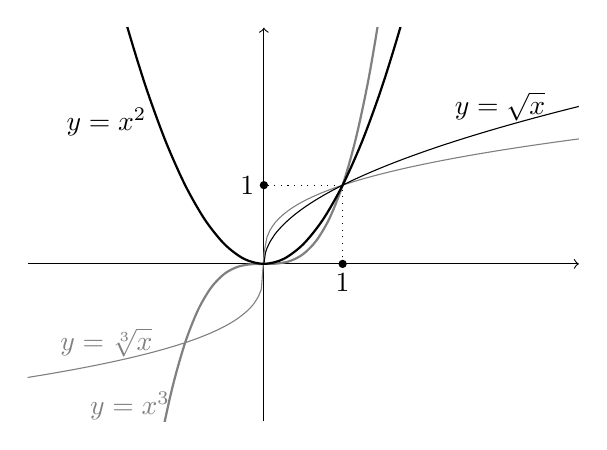
\begin{tikzpicture}[x=1.0cm,y=1.0cm]
      \clip(-3,-2) rectangle (4,3);
    	\draw[->] (-3,0) -- (4,0);
      \draw[->] (0,-2) -- (0,3);
      \draw[dotted] (1,0) -- (1,1) -- (0,1);
%      \draw[domain=0.2:4,samples=50,variable=\x,dashed,color=gray] plot
%        ({\x}, {1/(\x))});
%      \draw[domain=-3:-0.5,samples=50,variable=\x,dashed,color=gray] plot
%        ({\x}, {1/(\x))});
      \draw[domain=-2.0:2.0,smooth,variable=\x,thick,color=gray] plot
        ({\x}, {\x*\x*\x)});
      \draw[domain=-3.1:4.0,samples=200,variable=\x,color=gray] plot
        ({\x}, {pow(abs(\x),1/3)*\x / abs(\x)});
      \draw[domain=-3.0:3.0,smooth,variable=\x,thick] plot
        ({\x}, {\x*\x});
      \draw[domain=0.0:4.0,samples=200,variable=\x] plot
      ({\x}, {pow(\x,1/2)});
      \node at (-2.0,1.8) {$y=x^2$};
      \node at (3,2) {$y=\sqrt{x}$};
      \node[color=gray] at (-1.7,-1.8) {$y=x^{3}$};
      \node[color=gray] at (-2.0,-1) {$y=\sqrt[3]{x}$};
      \fill (1,0) node[below]{$1$} circle[radius=1.5pt];
      \fill (0,1) node[left]{$1$} circle[radius=1.5pt];
    \end{tikzpicture}
  \end{center}
  \caption{Grafici delle potenze $x^2$, $x^3$ e radici
  $\sqrt x$, $\sqrt[3] x$.}
  \label{fig:potenza_intera_radice}
\end{figure}

\subsection{l'insieme dei numeri naturali $\NN \subset \RR$}
%
\index{naturali!$\NN$ dentro $\RR$}%
\index{numeri!naturali $\NN$ dentro $\RR$}%
\index{$\NN$}%

Fin'ora abbiamo considerato gli insiemi $\NN$ 
e $\RR$ come insiemi scorrelati. 
I numeri naturali $0\in \NN$ e $1=\sigma(0)\in \NN$ 
sono in generale diversi dai numeri reali 
$0\in \RR$ (elemento neutro dell'addizione) 
e $1\in \RR$ (elemento neutro della moltiplicazione).

Sarebbe sensato tenere distinti questi due insiemi numerici 
ma in pratica risulta comodo identificare i numeri naturali 
come particolare sottoinsieme dei numeri reali.
Su $\RR$ possiamo definire la funzione (traslazione a destra di una unità)
$\sigma\colon \RR\to\RR$, $\sigma(x) = x+1$.
Vorremmo quindi considerare l'insieme che si ottiene 
partendo da $0\in \RR$ e considerando tutti gli elementi che si
ottengono iterando la funzione $\sigma$: $1=\sigma(0)$, $2=\sigma(1)$, \dots

Formalmente questo si ottiene mediante una definizione:
diremo che un sottoinsieme $A\subset \RR$ è \emph{induttivo}
se soddisfa le seguenti proprietà:
\index{insieme!induttivo}%
\mymargin{insieme induttivo}%
\begin{enumerate}
  \item $0\in A$;
  \item $x\in A \implies x+1 \in A$.
\end{enumerate}

Possiamo allora definire i numeri naturali (dentro $\RR$) come 
il \emph{più piccolo} sottoinsieme induttivo di $\RR$:
\[
 \NN = \bigcap\ENCLOSE{A\subset \RR \colon \text{$A$ induttivo}}.  
\]
Ovviamente l'insieme $\RR$ stesso è un insieme induttivo, 
dunque la famiglia di insiemi su cui stiamo facendo l'intersezione,
non è vuota e dunque l'intersezione è ben definita.
Inoltre l'insieme risultante è a sua volta induttivo:
visto che $0$ è elemento di tutti gli insiemi induttivi, 
certamente $0$ deve stare nella loro intersezione; 
e se $x$ sta nell'intersezione di tutti gli insiemi induttivi 
allora anche $x+1$ sta in ogni insieme induttivo e quindi 
nella loro intersezione. 
La funzione $\sigma\colon \RR\to\RR$ è iniettiva e dunque 
possiamo affermare che le prime due proprietà degli assiomi 
di Peano (definizione~\ref{def:naturali}) sono soddisfatte.
Ma anche l'assioma di induzione è soddisfatto in quanto 
se prendiamo un qualunque sottoinsieme induttivo di $\NN$ 
questo non può che essere uguale ad $\NN$ perché $\NN$, 
per definizione di intersezione, è contenuto in ogni 
sottoinsieme induttivo di $\RR$ (e quindi in ogni 
sottoinsieme induttivo di se stesso).


\subsection{l'insieme dei numeri interi $\ZZ \subset \RR$}
%
%
\index{interi!$\ZZ$ dentro $\RR$}%
\index{numeri!interi $\ZZ$ dentro $\RR$}%
\index{$\ZZ$}%

Avendo posto $\NN\subset \RR$ possiamo definire facilmente i numeri interi
$\ZZ \subset \RR$ 
ponendo $\ZZ = \NN - \NN$
cioè l'insieme di tutte le possibili somme tra i numeri naturali 
e i loro opposti. Si può facilmente verificare che 
\[
 \ZZ = \NN \cup (-\NN)  
\]
perché ogni differenza $n-m$ di numeri naturali 
è un numero naturale se $n\ge m$ ed è l'opposto 
di un numero naturale $n-m = -(m-n)$ se $n\le m$.
Dunque $\ZZ$ si ottiene aggiungendo ai numeri naturali 
$n\in \NN\subset \RR$ i loro opposti $-n\in \RR$.

In questo modo $\ZZ$ risulta essere un gruppo additivo
rispetto alla operazione di addizione ereditata da $\RR$.
Infatti la somma di due numeri in $\ZZ$ è ancora 
un numero in $\ZZ$:
\[
  (n-m) + (n'-m') = (n+n') - (m+m')
  \qquad\text{($n,m,n,m'\in \NN)$.}
\]

L'insieme numerico $\ZZ$ eredita da $\RR$ anche 
l'ordinamento e tale ordinamento è compatibile con l'addizione 
perché lo era in $\RR$. Dunque $\ZZ$ risulta essere un gruppo 
totalmente ordinato.
Però $\ZZ$ non è denso perché si può dimostrare che 
non esistono numeri interi strettamente compresi tra $0$ e $1$.
\mynote{
Se $0<x<1$ e per assurdo fosse $x\in \ZZ$ 
allora sarebbe $x\in \NN\setminus\ENCLOSE{0}$ in quanto $x>0$.
Ma $\NN\setminus\ENCLOSE{0} = \NN + 1$ quindi 
si avrebbe $x-1\in \NN$ che è assurdo in quanto $x-1<0$
se $x<1$.}
Si potrebbe anche dimostrare che $\ZZ$ è continuo (esercizio!),
fornendo dunque un esempio di gruppo totalmente ordinato, 
denso ma non continuo.

\subsubsection{parte intera}

\begin{theorem}[parte intera]
\mymark{*}%
  Dato $x\in \RR$ esiste un unico $m\in \ZZ$ tale che $m-1 < x \le m$.
\end{theorem}
%
\begin{proof}
  Supponiamo per un attimo che sia $x > 0$
  e consideriamo l'insieme $A=\ENCLOSE{n \in \NN \colon n\ge x}$.
  Tale insieme non è vuoto per la proprietà archimedea 
  e dunque ammette minimo per il principio del buon ordinamento.
  Se $m=\min A$ risulta quindi $m\in \NN$ e $m-1< x \le m$.

  Se $x\le 0$ per la proprietà archimedea esiste $k\in \NN$ tale che 
  $k>-x$. Allora applichiamo il risultato precedente a $x+k$ e consideriamo 
  $m-k$ al posto di $m$.
\end{proof}

\begin{definition}[parte intera]
  \mymark{**}%
  \mymargin{parte intera}%
\index{parte!intera}%
  Dato $x\in \RR$ denotiamo con $\lfloor x\rfloor$ l'unico intero
  che soddisfa
  \mymargin{$\lfloor\cdot\rfloor$} %% *** non viene bene nell'indice!
  \[
    x - 1 < \lfloor x \rfloor \le x
  \]
  e denotiamo con $\lceil x \rceil = - \lfloor -x \rfloor$ l'unico intero che soddisfa (verificare!)
  \mymargin{$\lceil\cdot\rceil$} %% *** non viene bene nell'indice!
  \[
    x \le \lceil x \rceil < x + 1.
  \]
  Si ha dunque
  \[
    \lfloor x \rfloor \le x \le \lceil x \rceil
  \]
  con entrambe le uguaglianze che si realizzano quando $x\in \ZZ$.
  I due interi $\lfloor x \rfloor$ e $\lceil x \rceil$
  sono la migliore approssimazione intera di $x$ rispettivamente
  per difetto e per eccesso.
  L'intero più vicino ad $x$ (approssimazione per \emph{arrotondamento}%
\mymargin{arrotondamento}%
\index{arrotondamento})
  è
  \[
    \left\lfloor x + \frac 1 2 \right\rfloor
  \quad \text{ossia} \quad
    \left\lceil x-\frac 1 2 \right\rceil
  \]
  (le due espressioni differiscono solamente quando $x$ si trova nel punto medio tra 
  due interi consecutivi, nel qual caso la prima approssima per eccesso e la seconda 
  per difetto).
\end{definition}

In alcuni testi si usa la notazione $[x]$ per denotare la parte intera $\lfloor x \rfloor$ e si definisce
anche la \emph{parte frazionaria}
\[
  \ENCLOSE{x} = x - [x].
\]
Per evitare ambiguità con il normale utilizzo delle parentesi
non useremo queste notazioni.

\subsection{l'insieme dei numeri razionali $\QQ\subset \RR$}
%
%
\index{razionali!$\QQ$ dentro $\RR$}%
\index{numeri!razionali $\QQ$ dentro $\RR$}%
\index{$\QQ$}%

Per ogni $m\in \ZZ$ ed ogni $n\in \ZZ$ se $n\neq 0$ è ben
definito il quoziente $\frac m n\in \RR$.
Definiamo allora l'insieme $\QQ\subset \RR$ di tutte le frazioni:
\[
    \QQ = \frac{\ZZ}{\ZZ\setminus\ENCLOSE{0}}.
\]
Si può verificare che $\QQ$ è un gruppo additivo in quanto 
la somma di frazioni è ancora una frazione:
\[
  \frac{m}{n} + \frac{m'}{n'}
  = \frac{mn'}{nn'} + \frac{m'n}{nn'} 
  = \frac{mn'+nm'}{n n'}
\]
e, ovviamente, l'opposto di una frazione è una frazione: 
$- \frac m n = \frac{-m}{n}$. 
Inoltre $\QQ\setminus \ENCLOSE{0}$ è un gruppo 
additivo in quanto anche il prodotto di due frazioni 
è ovviamente una frazione, e lo stesso vale per il reciproco di frazioni 
non nulle:
\[
  \frac{m}{n}\cdot \frac{m'}{n'} = \frac{m\cdot m'}{n\cdot n'},
  \qquad
  \frac{1}{\frac m n} = \frac n m.  
\]
L'ordinamento di $\RR$ viene ereditato da $\QQ$ ed è quindi ovviamente 
compatibile con le operazioni di addizione e moltiplicazione. 
Risulta quindi che $\QQ$ è un esempio di campo ordinato, come $\RR$.
Ovviamente $\QQ$ è denso come ogni campo ordinato.

\subsubsection{numeri irrazionali}

Se l'ordinamento di $\QQ$ fosse continuo il teorema 
di isomorfismo ci direbbe 
che c'è un unico omomorfismo positivo $f\colon \QQ \to \RR$ 
tale che $f(1)=1$. 
Ma l'inclusione $x\mapsto x$ è anch'esso un omomorfismo positivo 
di $\QQ \to \RR$ e dunque dovrebbe coincidere con $f$.
Ma il teorema ci dice anche che tale $f$ è bigettiva dunque 
si avrebbe $\RR = f(\QQ) = \QQ$.
E' rilevante osservare che questo non accade e cioè 
$\QQ\neq \RR$ perché $\QQ$ non è continuo. 
Il primo ad accorgersene fu, per quanto ne sappiamo,
Pitagora che dimostrò che $\sqrt 2$
non è un numero razionale, dunque $\sqrt 2 \in \RR \setminus \QQ$.

Visto che i numeri di $\QQ$ si chiamano \emph{razionali} (da \emph{ratio}, rapporto)
gli elementi di $\RR\setminus \QQ$ si chiamano \emph{irrazionali} e $\sqrt 2$ 
è il primo esempio di tale casistica.

Possiamo enunciare l'irrazionalità di $\sqrt 2$ 
senza tirare in ballo i numeri reali, 
dimostrando che l'equazione $x^2=2$ non ha soluzioni in $\QQ$.

\begin{theorem}[Pitagora, irrazionalità di $\sqrt 2$]
  \mymark{**}%
  \label{th:pitagora}%
  L'equazione $x^2=2$ non ha soluzioni in $\QQ$.
  \end{theorem}
  %
  \begin{proof}
  \mymark{*}%
  Supponiamo $x\in \QQ$ sia una soluzione di $x^2=2$.
  Allora si potrà scrivere $x=p/q$ con $p\in \ZZ$ e $q\in \NN$, $q\neq 0$.
  Possiamo anche supporre che la frazione $p/q$ sia ridotta ai minimi
  termini cioè che $p$ e $q$ non abbiano fattori in comune.
  Moltiplicando l'equazione
  $(p/q)^2=2$ per $q^2$ si ottiene $p^2 = 2 q^2$.
  Risulta quindi che $p^2$ è pari.
  Ma allora anche $p$ è pari (perché il quadrato di un dispari è dispari).
  Ma se $p$ è pari allora $p^2$ è multiplo di quattro.
  Ma allora anche $2q^2$ è multiplo di quattro e quindi $q^2$ è pari.
  Dunque anche $q$ è pari. Ma avevamo supposto che $p$ e $q$ non avessero
  fattori in comune quindi questo non può accadere.
\end{proof}

Abbiamo quindi dimostrato che $\QQ$ non può essere continuo (altrimenti 
sarebbe isomorfo a $\RR$ dove l'equazione $x^2=2$ ha soluzione). 
Utilizzando l'irrazionalità di $\sqrt 2$ 
possiamo ora esibire un esempio di sottoinsiemi di $\QQ$ che sono 
\emph{separati} (nel senso della definizione~\ref{def:ordinamento_continuo})
ma non hanno elemento di separazione in $\QQ$:
\[
A= \ENCLOSE{x\in\QQ\colon x^2< 2},
\qquad
B = \ENCLOSE{x\in \QQ\colon x<0, x^2>2}.  
\]
Chiaramente $A\le B$ ma in $\RR$ questi due insiemi 
hanno come unico elemento di separazione $\sqrt 2$ che non è elemento di
$\QQ$.

Abbiamo appena verificato che esistono numeri irrazionali. 
Può però essere sorprendente scoprire che non solo i numeri irrazionali 
sono infiniti (chiaramente se $x$ è irrazionale anche $n\cdot x$ è irrazionale 
se $n$ è intero o razionale) ma addirittura la cardinalità 
dei numeri irrazionali è maggiore di quella dei numeri razionali 
$\# (\RR\setminus \QQ) > \# \QQ$ (teorema~\ref{th:cantor_secondo}).

Ogni numero razionale ha una rappresentazione finita. 
Se $x=\frac p q$ possiamo scrivere $p$ e $q$ nella loro rappresentazione 
decimale utilizzando una sequenza finita di cifre.
Possiamo dare \emph{un nome} anche a molti
numeri irrazionali. 
Ad esempio $\sqrt 2$, $e$, $\pi$, $\sin 1$, $\ln 2$ identificheranno 
alcuni numeri irrazionali. 
Ma non è possibile dare una rappresentazione \emph{finita} di ogni numero reale.
Per questo motivo è rilevante il fatto che i numeri razionali siano \emph{densi}
nei numeri reali perché questo significa che ogni numero reale può essere 
approssimato, con un errore piccolo a piacere, tramite un numero razionale.

\begin{theorem}[densità di $\QQ$ in $\RR$]
\label{th:densita_frazioni}%
\index{densità!frazioni}%
\index{approssimazioni!decimali}%
Dati $a,b\in \RR$ se $a<b$ esiste $q\in \QQ$ tale che $a< q < b$.

Equivalentemente dato $x\in \RR$ e dato $\eps>0$ esiste $q\in \QQ$ 
tale che $\abs{x-q} < \eps$.

Inoltre la frazione $q= \frac{p}{n}$ può essere scelta 
in modo tale che il denominatore sia una potenza di $10$: $n=10^k$.
\end{theorem}
\begin{proof}
La prima parte è conseguenza della seconda perché 
dati $a<b$
se scegliamo 
$x= \frac{a+b}{2}$ ed $\eps = \frac{b-a} 2$ se 
esiste $q$ tale che $\abs{x-q}< \eps$ 
allora 
\[
   a = \frac{a+b}{2} - \eps < q < \frac{a+b}{2} + \eps = b.
\]

Per dimostrare la seconda parte dati $x$ e $\eps$ basterà scegliere 
$n\in \NN$ tale che $\frac 1 n < \eps$ (l'esistenza di $n$ è garantita 
dal teorema~\ref{th:archimede}, proprietà archimedea) e predere $q = \frac{\lfloor nx\rfloor}{n}$
cosicché, per le proprietà della parte intera, si ha:
\[
  nx-1\le \lfloor nx\rfloor \le nx 
  \qquad\text{e quindi}\qquad
  x - \frac 1 n \le q \le x
\]
da cui $0 \le x-q < \frac 1 n < \eps$ come volevamo dimostrare.

Per avere una frazione con denominatore potenza di $10$ basta osservare 
che se aumentiamo $n$ la precisione della approssimazione aumenta. 
Dunque basta osservare che per ogni $n\in \NN$ esiste $d\in \NN$
tale che $10^d \ge n$ (basta scegliere $d=n$ e dimostrare per induzione 
che $10^n\ge n$).
\end{proof}

\begin{exercise}\label{ex:densita_irrazionali}
  Dimostrare che anche gli irrazionali 
  sono densi in $\RR$ cioè che se $a<b$ allora esiste 
  $x \in \openinterval{a}{b}$, $x\not \in \QQ$.
\end{exercise}

\subsubsection{frazioni decimali}
%
Le frazioni il cui denominatore è una potenza
di $10$ si chiamano frazioni decimali:
\[
  x = \frac{p}{10^d}, \qquad p\in \ZZ, d\in \NN.
\]
Tali frazioni si possono rappresentare
scrivendo il numero
intero $p$ e segnando un punto
\mynote{%
in Italia si preferisce utilizzare la virgola, ma
ci rassegnamo alla notazione anglosassone che ormai è
ubiqua in tutta la strumentazione elettronica.
}%
di separazione
prima della $d$-esima cifra a partire da destra.
Ad esempio scriveremo:
\[
  1.4142 = \frac{14142}{10^4}.
\]
In generale una frazione $\frac{p}{q}\in \QQ$
può essere scritta in forma decimale solamente
se, quando ridotta ai minimi termini,
risulta che $q$ non ha fattori primi diversi
da $2$ e $5$ (in quanto le potenze di dieci
hanno solo questi fattori).

Anche se non tutte le frazioni hanno una rappresentazione 
decimale finita, in ogni caso le frazioni decimali 
sono dense in $\RR$ (come dimostrato nel teorema~\ref{th:densita_frazioni})
e quindi ogni numero reale può essere approssimato, con errore piccolo a piacere,
mediante una frazione decimale.

Scriveremo
\mymargin{$\approx$}%
\index{$\approx$}%
\[
  x \approx \frac{p}{10^d}
\]
(si può leggere: ``$x$ è approssimativamente uguale a\dots'')
se
\[
    \frac{p-1}{10^d} < x < \frac{p+1}{10^d}.
\]

Ad esempio possiamo scrivere
\[
  \sqrt 2 \approx 1.41 = \frac{141}{10^2}
\]
per intendere%
\mynote{%
Si osservi che in base alla definizione data sarebbe anche corretto 
scrivere $\sqrt 2 \approx 1.42$ che però è una approssimazione 
peggiore. 
Questa ambiguità è necessaria se vogliamo evitare i casi 
limite in cui bisogna conoscere molte più cifre decimali di quelle richieste 
per capire qual è la migliore approssimazione.
}%
\begin{equation}\label{eq:approx_sqrt2}
\frac{140}{100} < \sqrt 2 < \frac{142}{100}.
\end{equation}
Nel calcolo numerico scientifico ogni uguaglianza numerica è intesa nel 
senso precedente, se non specificato diversamente. 

\begin{exercise}
Dimostrare \ref{eq:approx_sqrt2} senza 
utilizzare la calcolatrice.
\end{exercise}

Osserviamo infine che anche i calcolatori utilizzano una rappresentazione frazionaria, 
nel caso specifico \emph{binaria}, dei numeri.
I numeri frazionari su cui opera un calcolatore sono tutti della forma $\frac{p}{2^d}$.
Visto che $2$ divide $10$, le frazioni binarie sono anche sempre frazioni decimali, 
in particolare anche questi numeri sono densi in $\RR$.
\mynote{In un moderno calcolatore a 64 bit la rappresentazione binaria (float64) 
utilizza frazioni binarie con esponente $d\le 1024$. 
Questo permette di rappresentare numeri con una precisione non superiore alle 
$308$ cifre decimali. 
La rappresentazione è a virgola mobile e quindi questa precisione si può raggiungere 
solamente con numeri vicini allo zero, per numeri vicini a $1$ 
si ha invece $d\le 53$ che corrisponde ad una precisione di quasi $16$ cifre decimali.}

\subsubsection{frazioni decimali periodiche}

Le frazioni non decimali si possono scrivere con uno sviluppo
decimale \emph{periodico}. 
Non useremo mai questa notazione
che ricordiamo solamente con un esempio.
Il numero
\[
  x = 12.34\overline{567}
    = 12.34567\overline{567}
\]
è la frazione $x$ che risolve l'equazione
\[
  \frac{100x - 1234}{1000}
  = 100x-1234.567
  \qquad
\enclose
{\frac{0.\overline{567}}{1000}
= 0.000\overline{567} }
\]
ovvero
\[
  1234567 - 1234 = 99900 \cdot x,
  \qquad x = \frac{1234567-1234}{99900}.
\]

\begin{exercise}
Si verifichi che $0.\overline 9 = 1$.
\end{exercise}
    
Per passare dalla rappresentazione frazionaria alla rappresentazione 
decimale periodica basta svolgere la divisione in colonna.
Se l'algoritmo termina la frazione era decimale, altrimenti l'algoritmo 
diventa periodico e le cifre decimali si ripetono indefinitamente.

\subsection{estremo superiore, estremo inferiore}

\begin{definition}[maggiorante, minorante, massimo, minimo, limitato]
  \mymark{***}%
  \label{def:minorante}%
  \label{def:maggiorante}%
  \label{def:minimo}%
  \label{def:limitato}%
  % Sia $\le$ una relazione d'ordine su un insieme $X$ e siano 
  Siano $x\in \RR$ e $A\subset \RR$.

  Diremo che $x$ è un \emph{minorante}%
\mymargin{minorante}%
\index{minorante} di $A$ e scriveremo:
  \[
    x \le A
  \]
  se per ogni $a\in A$ risulta $x\le a$. 
  Se esiste $x$ per cui $x\le A$ diremo che $A$ 
  è \emph{inferiormente limitato}.
  \index{inferiormente!limitato}%
  \index{limitato!inferiormente}%
  Se $x$ è un minorante e inoltre $x\in A$ diremo 
  che $x$ è il \emph{minimo}%
\mymargin{minimo}%
\index{minimo} di $A$ e scriveremo:
  \[
    x = \min A.  
  \] 

  Analogamente diremo che $x$ è un \emph{maggiorante}%
\mymargin{maggiorante}%
\index{maggiorante}
  di $A$ e scriveremo $x \ge A$ se $x\ge a$ per ogni $a\in A$,
  diremo che $A$ è \emph{superiormente limitato} 
  \index{superiormente!limitato}%
  \index{limitato!superiormente}%
  se esiste $x$ per cui $x \ge A$ infine
  diremo che $x$ è il \emph{massimo}%
\mymargin{massimo}%
\index{massimo} di $A$ 
  e scriveremo $x=\max A$ se $x\ge A$ e $x\in A$.

  Se $A$ è superiormente limitato e inferiormente limitato
  diremo che $A$ è \emph{limitato}.
  \mymargin{limitato}%
  \index{limitato}%
  
  Se $A$ non è limitato diremo che $A$ è \emph{illimitato}.
\end{definition}

Massimo e minimo di un insieme $A$, se esistono, sono unici.
Infatti se $x$ e $y$ fossero due minimi di $A$ si avrebbe $x\le y$ in
quanto $x\le A$ e $y\in A$. Analogamente si avrebbe $y\le x$ e
quindi $x=y$. Ragionamento analogo se $x$ e $y$ fossero due massimi.

\mynote{
  Se $A$ è un insieme finito il massimo e il minimo 
  esistono sempre. 
  Se $A$ non avesse minimo potrei definire per induzione 
  una funzione $f\colon \NN\to A$ tale che $f(0)\in A$ 
  è qualunque e $f(n+1) < f(n)$ (visto che $f(n)$ non è un minimo 
  di $A$ esiste un numero più piccolo). 
  Chiaramente $f$ è iniettiva quindi $\#A\ge \#\NN$
  e dunque $A$ è infinito.
  Se invece $A$ è infinito il massimo e il minimo 
  potrebbero non esistere. 
  Ad esempio l'insieme $A=\ENCLOSE{x\in \RR\colon 0<x<1}$
  non ha né massimo né minimo.
}

\mynote{
  Non si confonda il concetto di \emph{insieme infinito} 
  con quello di \emph{insieme illimitato}.
  Un insieme infinito può essere illimitato: si 
  prenda ad esempio l'insieme $A=\ENCLOSE{x\in \RR\colon 0\le x \le 1}$
  che è chiaramente limitato ma è infinito perché contiene,
  ad esempio, tutti i numeri $\frac{1}{n}$ con $n\in\NN$.
}

\begin{definition}%
  Se $x$ è il minimo dei maggioranti di $A$ diremo che $x$ è
  l'\emph{estremo superiore}%
\mymargin{estremo superiore}%
\index{estremo!superiore}%
  di $A$ se invece $x$ è il massimo dei minoranti diremo che $x$ è
  l'\emph{estremo inferiore}%
\mymargin{estremo inferiore}%
\index{estremo!inferiore} di $A$:
  \begin{align*}
  \sup A &= \min \ENCLOSE{x\in \RR \colon x\ge A}, \\
  \inf A &= \max \ENCLOSE{x\in \RR \colon x \le A}.
  \end{align*}
  \index{$\sup$}%
  \index{$\inf$}%
  \index{sup}%
  \index{inf}%
\end{definition}

\begin{theorem}[esistenza del $\sup$]%
  \label{th:sup}%
  \mymark{**}%
  Se $A\subset \RR$ è un insieme non vuoto
  e superiormente limitato, allora esiste l'estremo superiore di $A$.
  Se $A\subset \RR$ è un insieme non vuoto e inferiormente limitato 
  allora esiste l'estremo inferiore di $A$.
  \end{theorem}
  %
  \begin{proof}
  \mymark{*}
  Consideriamo l'insieme dei maggioranti
  \[
  B = \ENCLOSE{ b\in \RR \colon b \ge A}.
  \]
  Per ipotesi $B$ è non vuoto e per come è definito risulta $A\le B$.
  Dunque dall'assioma di continuità (definizione~\ref{def:ordinamento_continuo}) 
  deduciamo l'esistenza di un numero $x\in \RR$
  tale che $A\le x \le B$. La prima disuguaglianza $A\le x$ ci dice che $x$ è un
  maggiorante e quindi $x\in B$, la seconda $x\le B$ ci dice che $x$ è il minimo
  di $B$ e quindi concludiamo che $x$ è il minimo dei maggioranti 
  ovvero l'estremo superiore di $A$.

  Dimostrazione analoga vale per l'estremo inferiore.
\end{proof}

L'esistenza del $\sup$ (o dell'$\inf$)
è in effetti una condizione equivalente all'assioma di continuità.
Infatti se $A\le B$ certamente $\sup A$, se esiste, è elemento 
di separazione tra $A$ e $B$.

\subsection{punti all'infinito}
\label{sec:reali_estesi}
%%%%%%%%%%%%%%%%%%%
%%%%%%%%%%%%%%%%%%%
%%%%%%%%%%%%%%%%%%%

\begin{definition}[reali estesi]
\mymargin{$\bar\RR$}%
\index{$\bar{\RR}$}
Denotiamo con $\bar \RR=\RR \cup \ENCLOSE{+\infty, -\infty}$ l'insieme dei numeri reali
\mymargin{$+\infty$, $-\infty$}%
\index{$+\infty$, $-\infty$}
a cui vengono aggiunti due ulteriori \emph{quantità} che chiameremo
\emph{infinite} e che denotiamo con $+\infty$ e $-\infty$.
Diremo che $x\in \bar \RR$ è \emph{finito} se $x\in \RR$.
\end{definition}


Estendiamo la relazione d'ordine imponendo che valga
\[
  -\infty \le x \le +\infty, \qquad \forall x \in \bar\RR.
\]

Estendiamo anche la addizione e moltiplicazione
tra reali estesi imponendo che valga per ogni $x\in \bar \RR$
\begin{gather*}
  x + (+\infty) = +\infty, \qquad \text{se $x\neq -\infty$}\\
  x + (-\infty) = -\infty, \qquad \text{se $x\neq +\infty$}\\
  x \cdot (+\infty) = +\infty, \qquad
  x \cdot (-\infty) = -\infty, \qquad \text{se $x>0$} \\
  x \cdot (+\infty) = -\infty, \qquad
  x \cdot (-\infty) = +\infty, \qquad \text{se $x<0$}.
\end{gather*}

Si definiscono anche:
\[
 -(+\infty) = -\infty, \qquad
 -(-\infty) = +\infty, \qquad
 \frac{1}{+\infty} = \frac{1}{-\infty}=0
\]
facendo però attenzione che
questi formalmente non sono \emph{opposto}
e \emph{reciproco} in quanto
su $\bar \RR$ non sono più garantite
le regole: $x + (-x) = 0$ e $x \cdot (1/x) = 1$.
Infatti
le operazioni $(+\infty) + (-\infty)$ e $+\infty \cdot 0$ vengono
lasciate indefinite.

Definiamo anche il valore assoluto: $\abs{+\infty} = \abs{-\infty} = +\infty$.

Possiamo infine definire la sottrazione e la divisione tramite
addizione e moltiplicazione:
\[
  x - y = x + (-y), \qquad \frac{x}{y} = x \cdot \frac{1}{y}.
\]

Possiamo definire gli operatori $\sup$ e $\inf$
anche sugli insiemi illimitati ponendo:
\begin{align*}
  \sup A = +\infty \qquad \text{se $A$ non è superiormente limitato}\\
  \inf A = -\infty \qquad \text{se $A$ non è inferiormente limitato}.
\end{align*}
Osserviamo infatti che su $\bar \RR$ la quantità $+\infty$
è maggiorante di qualunque insieme e $-\infty$ è minorante, dunque
queste definizioni mantengono su $\bar \RR$ le proprietà caratterizzanti:
l'estremo superiore è il minimo dei maggioranti e
l'estremo inferiore è il massimo dei minoranti.
Definiamo infine
\begin{align*}
  \sup \emptyset = -\infty\\
  \inf \emptyset = +\infty.
\end{align*}
Queste ultime definizioni possono essere comprese da un punto di vista
strettamente logico: ogni numero reale è sia maggiorante che minorante
dell'insieme vuoto, dunque il minimo dei maggioranti non esiste in $\RR$
ma in $\bar \RR$ è $-\infty$
e il massimo dei minoranti è $+\infty$.

\subsection{intervalli}

\begin{definition}[intervallo]
\label{def:intervallo}%
\mymargin{intervallo}%
\index{intervallo}%
Un insieme $I\subset \bar\RR$ si dice essere un \emph{intervallo}
se contiene tutti i punti intermedi:
\[
  \text{se $x, y \in I$ e $x<z<y$ allora $z \in I$.}
\]
\end{definition}
%
\begin{theorem}[caratterizzazione intervalli di $\RR$]
Sia $I\subset \RR$ un intervallo e siano $a=\inf I$, $b=\sup I$
i suoi estremi. Allora
$z\in I$ se $a < z < b$.
\end{theorem}
%
\begin{proof}
Se $I=\emptyset$ si ha $a>b$ e quindi nessuno $z$ verifica $a<z<b$.
Supponiamo $I\neq \emptyset$ e
sia $a < z < b$.
Visto che $a$ è il massimo dei minoranti di $I$
il numero $z$ non è un minorante dunque
deve esistere $x \in I$ tale
che $x < z$. Analogamente dovrebbe esistere $y\in I$
con $z<y$.
Ma allora, per definizione di intervallo, anche $z\in I$.
\end{proof}

Il teorema precedente ci dice che una volta identificati i due estremi
di un intervallo, tutti i punti intermedi devono stare nell'intervallo.
Gli estremi, invece, possono essere o non essere inclusi nell'intervallo.
Punti esterni agli estremi non possono invece essere elementi dell'intervallo.
Possiamo quindi caratterizzare tutti gli intervalli di $\RR$
introducendo le seguenti notazioni. Dati $a,b\in \bar \RR$ con $a\le b$
tutti i possibili intervalli con estremi $a$ e $b$ sono i seguenti:
\begin{equation}\label{eq:499494}
\begin{aligned}
\closeinterval{a}{b} &= \ENCLOSE{x\in \bar \RR\colon a \le x \le b} \\
\closeopeninterval{a}{b} &= \ENCLOSE{x\in \bar \RR\colon a \le x < b} \\
\opencloseinterval{a}{b} &= \ENCLOSE{x\in \bar \RR\colon a < x \le b}\\
\openinterval{a}{b} &= \ENCLOSE{x\in \bar \RR\colon a < x < b}.
\end{aligned}
\end{equation}
Abbiamo utilizzato le parentesi quadre per indicare che gli estremi
sono inclusi e le parentesi tonde per indicare che gli estremi sono esclusi.
Osserviamo che in alcuni testi si usano le parentesi quadre rovesciate al posto
delle parentesi tonde.

Se invece $a>b$ potremmo definire per convenzione:
\begin{equation}\label{eq:488364}
  [a,b] = [b,a], \quad
  [a,b) = (b,a], \quad
  (a,b] = [b,a), \quad
  (a,b) = (b,a).
\end{equation}
Si faccia però attenzione che in altri testi gli intervalli con gli estremi
scambiati non vengono definiti oppure vengono considerati vuoti.

La convenzione può essere utile perché in generale se $\vec a, \vec b$ sono
elementi di uno spazio vettoriale reale $V$ allora ha senso
definire:
\begin{align*}
    [\vec a,\vec b] &= \ENCLOSE{(1-t)\vec a + t \vec b\colon t\in [0,1]},\\
    [\vec a,\vec b) &= \ENCLOSE{(1-t)\vec a + t \vec b\colon t\in [0,1)},\\
    (\vec a,\vec b] &= \ENCLOSE{(1-t)\vec a + t \vec b\colon t\in (0,1]},\\
    (\vec a,\vec b) &= \ENCLOSE{(1-t)\vec a + t \vec b\colon t\in (0,1)}.
\end{align*}
L'intervallo $[\vec a,\vec b]$ è quindi il segmento di estremi
$\vec a$ e $\vec b$ e può essere definito anche se sullo spazio
vettoriale non è dato un ordinamento.
Questo rimane coerente con la definizione~\eqref{eq:499494}
data sopra solamente se adottiamo la convenzione~\eqref{eq:488364}.

Noi considereremo per lo più intervalli di $\RR$ (non di $\bar \RR$): in tal
caso gli estremi infiniti saranno sempre esclusi dall'intervallo.

\subsection{andamento del grafico di una funzione}
%
Se $f\colon A \subset \RR\to \RR$ è una funzione, un modo molto
utile di rappresentarla graficamente è quello di disegnarne il
grafico, ovvero la curva del piano cartesiano:
\[
   G_f = \ENCLOSE{(x,y)\in A\times \RR\colon y = f(x)}.
\]
Molte proprietà della funzione potranno essere riconosciute
geometricamente guardandone il grafico.

\begin{definition}[simmetrie]
Sia $f\colon A \subset \RR \to \RR$ una funzione.
Diremo che $f$ è:
\begin{enumerate}
\item \emph{pari}%
\mymargin{pari}%
\index{pari}
\index{funzione!pari}%
se $A=-A$ (significa che se $x\in A$ allora anche $-x\in A$) e
\[
  f(-x) = f(x);
\]
\item \emph{dispari}%
\mymargin{dispari}%
\index{dispari}
\index{funzione!dispari}%
se $A=-A$ e
\[
  f(-x) = -f(x);
\]
\item \emph{periodica}%
\mymargin{periodica}%
\index{periodico}
\index{funzione!periodica}%
di periodo $T$ se $A+T=A$
(significa che $x\in A \iff x+T \in A$)
se per ogni $x\in A$ si ha
\[
  f(x+T)=f(x)
\]
\end{enumerate}
\end{definition}

Ad esempio se $n\in \ZZ$ la funzione $f(x)=x^n$
è pari se $n$ è pari ed è dispari se $n$ è dispari.
Il grafico di una funzione dispari ha una simmetria
centrale, in quanto se $(x,f(x))\in G_f$ allora
anche $(-x,-f(x)) = (-x,f(-x))\in G_f$.
Il grafico di una funzione pari ha invece una
simmetria rispetto all'asse delle ordinate $x=0$
infatti se $(x,f(x))\in G_f$ allora $(-x,f(x)) = (-x,f(-x)) \in G_f$.

La funzione $f(x) = x - \lfloor x\rfloor$ (la parte frazionaria di $x$)
è un esempio di funzione periodica di periodo $T=1$. Infatti
è chiaro che $\lfloor x+1\rfloor = \lfloor x \rfloor +1$ e quindi
$f(x+1)=f(x)$.

Si osservi che \emph{dispari} per le funzioni non è la negazione
di \emph{pari}.
La funzione $f(x) = x+1$ non è né pari, né dispari, né periodica
(verificare).

\begin{definition}[zeri]
  Se $f\colon A\subset \RR \to \RR$ è una funzione diremo che
  $x\in A$ è uno \emph{zero} di $f$ se $f(x)=0$.
  L'\emph{insieme degli zeri}%
\mymargin{insieme degli zeri}%
\index{insieme!degli zeri}
  \index{zero!di una funzione}%
  è quindi dato da
  \[
    f^{-1}(\ENCLOSE{0}) = \ENCLOSE{x\in \RR\colon f(x) = 0}.
  \]
\end{definition}

Abbiamo già accennato al fatto che uno dei problemi più comuni in
matematica è quello di invertire una funzione. In particolare 
dato $y\in \RR$ ci si chiede quali siano gli $x\in \RR$ 
tali che $f(x)=y$. 
Questo problema si riconduce
a trovare gli zeri della funzione $f(x)-y$ e per questo motivo 
siamo interessati allo studio degli zeri.

Riprendiamo ora la definizione~\ref{def:monotonia} (monotonia) che da ora in avanti 
potrà essere applicata alle funzioni $f\colon A \to \RR$ definite 
su un insieme $A\subset \RR$.

Dal punto di vista grafico una funzione $f$ è crescente
se preso qualunque punto $(x,f(x))$ sul grafico della funzione
e tracciati gli assi paralleli agli assi cartesiani, passanti
per il punto fissato, si osserva che il grafico della funzione
è tutto contenuto nel primo e terzo quadrante determinati
dagli assi traslati.

E' facile verificare che la funzione $f\colon [0,+\infty)\to \RR$
definita da $f(x)=x^n$
è strettamente crescente se $n$ è un intero positivo.
Se però consideriamo la funzione definita su tutto
$\RR$: $f\colon \RR \to \RR$,
$f(x)=x^n$ allora solo se $n$ è dispari la funzione rimane
strettamente crescente
(le funzioni pari non possono mai essere strettamente crescenti se
il loro dominio contiene almeno tre punti distinti).

Se una funzione non è monotona è piuttosto comune studiare 
la monotonia della funzione ristretta a particolari intervalli: 
su alcuni intervalli la funzione (ristretta) potrà essere crescente e su altri 
intervalli potrà essere decrescente.

\begin{exercise}
Verificare che la composizione di funzioni monotone è una
funzione monotona e la composizione di funzioni strettamente
monotone è strettamente monotona.
Quando è che la funzione composta risulta crescente?
Quando decrescente?
\end{exercise}

\begin{exercise}
Si dimostri che applicando una funzione strettamente crescente ai due
membri di una equazione o disequazione (stretta o larga che sia)
si ottiene una equazione o disequazione equivalente.
Ovviamente è necessario che la funzione sia definita dove viene applicata.

Lo stesso vale per le funzioni strettamente decrescenti 
se però si cambia il verso della disequazione.
\end{exercise}

\begin{definition}[funzioni limitate, massimo/minimo]
\label{def:funzione_limitata}%
Se $f\colon A \to \RR$ è una funzione allora definiamo
l'estremo superiore di $f$ come l'estremo superiore
dell'immagine di $f$:
\[
  \sup f = \sup_{x\in A} f(x) = \sup f(A).
\]
In maniera analoga si definiscono l'estremo inferiore $\inf f$,
il massimo $\max f$ e il minimo $\min f$.

Dunque il massimo di una funzione è (se esiste) il valore massimo
che la funzione può assumere. I punti $x$ in cui
la funzione assume il valore massimo $f(x)$ vengono chiamati
\emph{punti di massimo}.
\mymargin{punto di massimo/minimo}%
\index{punto di massimo/minimo}%
\index{punto!di massimo}%
\index{punto!di minimo}%
Analogamente i punti in cui la funzione
assume il valore minimo (sempre che esistano) vengono
chiamati \emph{punti di minimo}.

Diremo che la funzione $f$ è
\emph{superiormente limitata}%
\mymargin{funzione superiormente limitata}%
\index{superiormente limitata}
se $\sup f<+\infty$
ovvero se esiste $M\in \RR$ tale che
\[
\forall x\in A \colon f(x) \le M.
\]
Diremo che la funzione $f$ è
\emph{inferiormente limitata}%
\mymargin{funzione inferiormente limitata}%
\index{inferiormente!limitato}
se $\inf f > -\infty$ ovvero se esiste $M\in \RR$ tale che
\[
 \forall x \in A \colon f(x) \ge M.
\]
Diremo che la funzione $f$ è \emph{limitata}%
\mymargin{funzione limitata}%
\index{limitata}
se è sia superiormente che inferiormente limitata ovvero
se $\sup\abs{f}<+\infty$ cioè se esiste $M\in \RR$ tale che
\[
\forall x \in A \colon \abs{f(x)}\le M.
\]
\end{definition}

Nel seguente esercizio abbiamo un esempio di funzione limitata.
\begin{exercise}
Si consideri la funzione $f\colon \RR\to\RR$
\[
 f(x) = \frac{1}{1+x^2}.
\]
Verificare che $\max f = \sup f = 1$, che $0$ è l'unico punto di massimo,
che $\inf f = 0$ e che $\min f$ non esiste.
\end{exercise}

\subsection{funzioni lineari}

\begin{figure}
  \begin{center}
    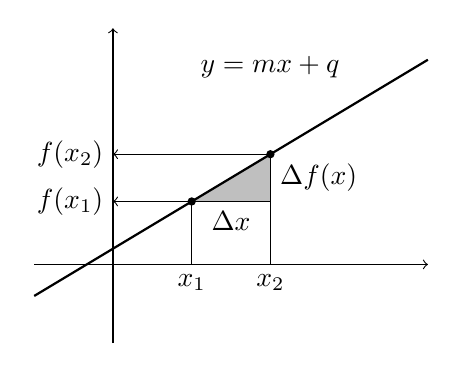
\begin{tikzpicture}[x=1.0cm,y=1.0cm]
    	\draw[->] (-1,0) -- (4,0);
      \draw[->] (0,-1) -- (0,3);
      % y = (3/5)*x + 1/5
      \fill[fill=lightgray,draw] (1,0.8) -- (2,0.8) node [midway,below]{$\Delta x$} -- (2,1.4) node [midway,right]{$\Delta f(x)$};
      \draw[thick] (-1,-0.4) -- (4,2.6);
      \draw[->] (1,0) node[below]{$x_1$} -- (1,0.8)
      -- (0,0.8) node[left]{$f(x_1)$};
      \draw[->] (2,0) node[below]{$x_2$} -- (2,1.4)
      -- (0,1.4) node[left]{$f(x_2)$};
      \fill (1,0.8) circle[radius=1.5pt];
      \fill (2,1.4) circle[radius=1.5pt];
      \node[left] at (3.0,2.5) {$y=mx+q$};
    \end{tikzpicture}
  \end{center}
  \caption{Il grafico di una funzione lineare.}
  \label{fig:funzione_lineare}
\end{figure}

Le \emph{funzioni lineari}%
\mymargin{funzione lineare}%
\index{funzioni lineari}
$f\colon \RR \to \RR$ sono le funzioni per le quali
esistono $m,q\in\RR$ tali che%
\mynote{%
Attenzione: nell'ambito dell'algebra lineare queste
funzioni verrebbero chiamate \emph{lineari affini}, mentre
le funzioni lineari dovrebbero sempre avere $q=0$.
Noi invece (come spesso accade nell'ambito dell'analisi)
chiameremo lineari queste funzioni e chiameremo
\emph{lineari omogenee} quelle con $q=0$.
Il termine \emph{lineare} pervade tutta la matematica 
e si applica in particolare alle equazioni che si ottengono 
tramite le funzioni lineari.
Purtroppo il nome scelto è fuorviante: la parola \emph{linea} viene 
usata a volte come abbreviazione di \emph{linea retta}, quando 
invece sarebbe più giusto utilizzare l'abbreviazione \emph{retta}
in quanto una linea può benissimo essere curva.
In altri contesti (come ad esempio nell'ambito degli ordinamenti)
il termine \emph{lineare} rappresenta un oggetto unidimensionale
senza ramificazioni ed è quindi maggiormente aderente 
al significato originale della parola.
} % marginnote
\[
  f(x) = mx + q.
\]

Se prendiamo due punti $(x_1,f(x_1))$
e $(x_2,f(x_2))$ sul grafico di una funzione lineare
possiamo osservare che si ha
\[
  \frac{f(x_2) - f(x_1)}{x_2 - x_1} = m.
\]
Il coefficiente $m$, dunque, rappresenta la pendenza del
grafico di $f$, ovvero il rapporto tra la variazione
dei valori della funzione $\Delta f = f(x_2) - f(x_1)$
e la variazione della variabile in ingresso
$\Delta x = x_2 - x_1$.
Geometricamente questo è il rapporto tra i due cateti
(base e altezza) che formano un triangolo rettangolo la
cui ipotenusa è il segmento che congiunge i due punti sul grafico.
Il fatto che questo rapporto sia costante significa,
in base al teorema di Talete, che i punti del grafico sono
allineati ovvero che il grafico di una funzione lineare è,
dal punto di vista geometrico, una retta.

\begin{definition}[retta]
  \index{retta}%
  \index{linea!retta}%
  Una \emph{linea retta} (più semplicemente: \emph{retta}) in è un sottospazio affine di dimensione 1 
  ovvero la traslazione di un sottospazio vettoriale di dimensione 1
  (si rimanda al corso di geometria).
\end{definition}

Tutte le rette del piano, 
tranne quelle parallele all'asse delle ordinate,
sono grafico di una funzione lineare.

Si osservi che per $m>0$ la funzione è strettamente crescente,
per $m=0$ la funzione è costante e per $m<0$ la funzione è
strettamente decrescente.

\subsection{funzioni quadratiche}
\label{sec:funzioni_quadratiche}

\begin{figure}
  \begin{center}
    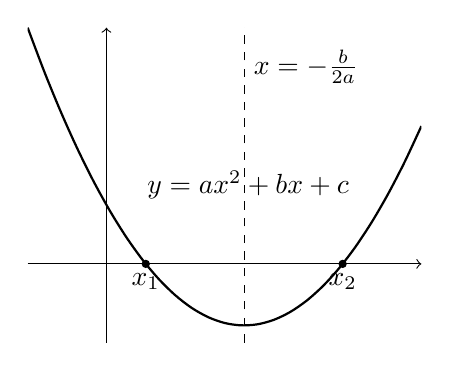
\begin{tikzpicture}[x=1.0cm,y=1.0cm]
      \clip(-1,-1) rectangle (4,3);
    	\draw[->] (-1,0) -- (4,0);
      \draw[->] (0,-1) -- (0,3);
      % y = (3/5)*x + 1/5
      \draw[dashed] (1.75,-1) -- (1.75,4);
      \node[right] at (1.75,2.5){$x=-\frac b {2a}$};
      \draw[domain=-1.0:4.0,smooth,variable=\x,thick] plot
      ({\x}, {0.5*(\x-0.5)*(\x-3.0)});
      \fill (0.5,0.0) node[below]{$x_1$} circle[radius=1.5pt];
      \fill (3,0.0) node[below]{$x_2$} circle[radius=1.5pt];
      \node at (1.8,1) {$y=ax^2+bx+c$};
    \end{tikzpicture}
  \end{center}
  \caption{Il grafico di una funzione quadratica.}
  \label{fig:funzione_quadratica}
\end{figure}

Le funzioni espresse mediante un \emph{polinomio di secondo grado}%
\mymargin{polinomio di secondo grado}%
\index{polinomio!di secondo grado}
\begin{equation}\label{eq:funzione_quadratica}
  f(x) = ax^2 + bx +c
\end{equation}
con $a,b,c\in \RR$, $a\neq 0$, si possono chiamare
\emph{funzioni quadratiche}%
\mymargin{funzioni quadratiche}%
\index{funzione!quadratica}.

Il modello di funzione quadratica è la funzione
$f(x) = x^2$ che (come tutte le potenze di esponente positivo e pari)
risulta essere una funzione pari, strettamente crescente
sull'intervallo $[0,+\infty)$ e strettamente decrescente
su $(-\infty,0]$. La funzione assume solamente valori non negativi
e si annulla solo per $x=0$.
Dunque l'equazione
\[
  x^2 = b
\]
non ha soluzione se $b<0$ ed ha come unica soluzione $x=0$ se $b=0$.
Se $b>0$ sappiamo che
questa equazione ha una unica soluzione positiva $x_1 = \sqrt{b}$
e, per simmetria, ha anche una soluzione negativa $x_2 = -\sqrt{b}$.
Sintetizzando si usa scrivere $x_{1,2} = \pm \sqrt{b}$
per unire in una unica riga le due definizioni.

La generica funzione quadratica~\eqref{eq:funzione_quadratica}
può essere ricondotta al caso modello tramite un cambio
di variabile lineare. In pratica si cerca di comporre il quadrato
di un binomio con un procedimento chiamato
\emph{completamento del quadrato}%
\mymargin{completamento del quadrato}%
\index{completamento del quadrato}:
\begin{equation}\label{eq:24589}
\begin{aligned}
f(x) = ax^2+bx+c
  &= a \Enclose{x^2+\frac b a x + \frac c a}\\
  &= a \Enclose{x^2+2 \frac{b}{2a} x + \frac{b^2}{4a^2} - \frac{b^2}{4a^2} + \frac c a}\\
  &= a \Enclose{\enclose{x+\frac{b}{2a}}^2 - \frac{b^2-4ac}{4a^2}} \\
  &= a\enclose{x+\frac b{2a}}^2  - \frac{b^2-4ac}{4a}.
\end{aligned}
\end{equation}

Ponendo $X=x+\frac b{2a}$ e $Y=y+\frac{b^2-4ac}{4a}$
l'equazione $y=ax^2+bx+c$ diventa quindi $Y=aX^2$. 
Significa
che il grafico della funzione quadratica~\eqref{eq:funzione_quadratica}
si ottiene traslando la curva $y = a x^2$ che, 
dal punto di vista geometrico, si può facilmente
dimostrare essere una parabola con fuoco
nel punto di coordinate $\enclose{0,\frac 1 {4a}}$
e asse la retta di equazione $x=0$.
Dunque il grafico di ogni funzione quadratica è una parabola, 
e più precisamente: ogni parabola con direttrice parallela all'asse delle
ascisse è il grafico di una funzione quadratica.

\begin{definition}[parabola]
  Una parabola con fuoco nel punto $\vec F=(F_1,F_2)\in \RR\times \RR$ 
  e retta direttrice 
  la retta $r \subset \RR\times\RR$ 
  è l'insieme dei punti  $\vec x = (x_1,x_2)\in \RR\times\RR$ 
  equidistanti da $\vec F$ e da $r$:
  \[
  \ENCLOSE{\vec x\in \RR\times\RR\colon 
  \sqrt{(x_1-F_1)^2 + (x_2-F_2)^2} 
  = \inf_{\vec P\in r}\sqrt{(x_1-P_1)^2+(y_1-P_1)^2}
  }.
  \]
\end{definition}

\begin{exercise}
  Si dimostri che per ogni $a\neq 0$ esiste $s\neq 0$ 
  per cui il riscalamento $X=sx$, $Y=sy$ porta il grafico della 
  parabola $y=ax^2$ nel grafico della parabola $Y=X^2$.
  Significa che 
  c'è una unica parabola 
  a meno di isometrie e riscalamenti.
\end{exercise}

Ricordando le proprietà di monotonia della funzione $X\mapsto X^2$
possiamo dedurre che se $a>0$ la funzione $f(x)$ è strettamente
decrescente se ristretta all'intervallo 
$\left(-\infty,-\frac b {2a}\right]$ ed è invece strettamente crescente 
sull'intervallo $\left[-\frac b{2a},+\infty\right)$. 
Ha dunque un punto di minimo in $x=-\frac{b}{2a}$.
Inoltre (sempre se $a>0$) la funzione è superiormente illimitata.
Viceversa se $a<0$ la funzione è inferiormente illimitata ed ha 
un massimo nel punto $x=-\frac{b}{2a}$.

E' molto importante saper risolvere equazioni e disequazioni
quadratiche. Grazie a~\eqref{eq:24589} l'equazione
\[
 a x^2 + bx + c = 0
\]
risulta equivalente a
\[
  \enclose{x+\frac{b}{2a}}^2 = \frac{b^2-4ac}{4a^2}.
\]
Dunque se $b^2-4ac<0$ l'equazione $ax^2+bx+c=0$ non ha soluzioni.
Se $b^2-4ac=0$ l'equazione ha una unica soluzione $x=-\frac{b}{2a}$.
Infine se $b^2-4ac>0$ si ottiene
\[
  x+\frac b{2a} = \pm \frac{\sqrt{b^2-4ac}}{2a}
\]
da cui la famosa formula risolutiva
\mymark{***}
\begin{equation}\label{eq:secondo_grado}
  x_{1,2} = \frac{-b \pm \sqrt{b^2-4ac}}{2a}.
\end{equation}

Risolvendo le disequazioni allo stesso modo, si trova
che la funzione $ax^2+bx+c$ quando $a>0$ è positiva
nei punti esterni alle soluzioni dell'equazione
(in tutti i punti se le soluzioni non esistono) ed
è negativa nei punti interni alle due soluzioni.
Viceversa se $a<0$ la funzione è positiva all'interno
delle due soluzioni e negativa all'esterno.


\subsection{funzioni esponenziali}
%
%
\label{sec:esponenziale}%

Il teorema di isomorfismo ci ha permesso di definire la moltiplicazione sui 
numeri reali. 
Lo stesso identico metodo ci permetterà di definire la funzione esponenziale
ovvero la potenza $a^x$ con base $a>0$ fissata ed esponente variabile $x\in \RR$.
Abbiamo infatti già osservato che l'insieme $\RR_+$ dei reali positivi
risulta essere un gruppo moltiplicativo totalmente ordinato, denso e continuo 
(teorema~\ref{th:gruppo_moltiplicativo}).

\begin{theorem}[funzione esponenziale]
  \label{th:esponenziale}%
Dato $a\in \RR$, $a\ge 1$ per ogni $x\in \RR$ si può definire in modo unico 
la funzione esponenziale $x\mapsto a^x$ con le seguenti proprietà:
\begin{enumerate}
  \item $a^1=a$;
  \item $a^{x+y} = a^x \cdot a^y$;
  \item per ogni $x\ge 0$ si ha $a^x\ge 1$.
\end{enumerate}
Se $0<a \le 1$ si può definire in modo unico l'esponenziale $x\mapsto a^x$ 
con le stesse proprietà, salvo che per ogni $x\ge 0$ si ha $a^x\le 1$.

Inoltre l'esponenziale ha le seguenti proprietà, 
valide per $a,b>0$, $x,y\in \RR$:
\begin{enumerate}
  \item $a^0=1$;
  \item $a^{-1} = \frac{1}{a}$;
  \item $(a\cdot b)^x = a^x\cdot b^x$;
  \item $(a^x)^y = a^{x\cdot y}$;
  \item $a^x \le a^y$ se $a\ge 1$ e $x\le y$;
  \item $1^x=1$.
\end{enumerate}
\end{theorem}
%
\begin{proof}
Fissato $a>0$ possiamo applicare il teorema~\ref{th:isomorfismo} (isomorfismo)
con $R=\RR$ gruppo additivo e $S=\RR_+$ gruppo moltiplicativo.
Se $a\ge 1$ si ottiene l'esistenza di una, unica, funzione $\phi_a\colon \RR \to \RR_+$ 
che soddisfa le seguenti proprietà:
$\phi_a(1)=a$, $\phi_a(x+y) = \phi_a(x)\cdot \phi_a(y)$, 
$\phi_a(x)\ge 1$ se $x\ge 0$. 
Se $0<a\le 1$ otteniamo una unica funzione con le stesse proprietà 
ma $\phi_a(x) \le 1$ se $x\ge 0$.

Definiamo $a^x = \phi_a(x)$ e la chiamiamo \emph{funzione esponenziale}
con \emph{base} $a>0$ ed esponente $x\in \RR$.
  
L'omomorfismo manda sempre l'elemento neutro nell'elemento 
neutro dunque $a^0 = 1$.
\mynote{Ricordiamo che in partenza abbiamo il gruppo additivo $\RR$
con elemento neutro $0$ mentre in arrivo 
abbiamo il gruppo moltiplicativo $\RR_+$ con elemento neutro $1$.}

\mymargin{$a^{-1}=\frac 1 a$}
Per la proprietà di omomorfismo si ha $a^{x-x} = a^x \cdot a^{-x}$
da cui $a^{-x}$ risulta essere il reciproco di $a^x$ cioè 
$a^{-x}= 1/a^x$.

Per la potenza del prodotto fissati $a,b\ge 1$ basta considerare la 
funzione $f(x) = a^x\cdot b^x$. 
\mymargin{$(a\cdot b)^x = a^x\cdot b^x$}
Chiaramente $f$ è un omomorfismo in quanto $a^x$ e $a^y$ lo sono 
(e il prodotto è commutativo): 
$a^{x+y}\cdot b^{x+y} = a^x \cdot b^x\cdot a^yb^y$.
Inoltre se $x\ge 0$ si ha $a^x\ge1$ e $b^x\ge 1$ da cui $f_(x)\ge 1$.
Essendo $f(1) = a^1\cdot b^1 = a\cdot b$ 
per l'unicità dell'omomorfismo positivo concludiamo che $f = \phi_{a\cdot b}$
cioè $a^x\cdot b^x = (a\cdot b)^x$.
Usando la regola del reciproco possiamo estendere questa proprietà 
quando $a<1$ e/o $b<1$ (ma sempre $a,b\ge 0$).

\mymargin{$(a^x)^y = a^{x\cdot y}$}
Infine per la potenza di potenza fissato $a\ge 1$ e $x\ge 0$ 
consideriamo la funzione $f(y) = a^{x\cdot y}$.
Per le proprietà precedenti si verifica facilmente che  
$f(y+z) = f(x)\cdot f(z)$. 
Inoltre se $a\ge 1$, $x\ge 0$ e $y\ge 0$ si ha 
$f(y)\ge 1$ che è la positività. 
Dunque per il teorema di isomorfismo,
essendo $f(1)=a^x$, si ottiene $f(y) = (a^x)^y$
che è quanto volevamo dimostrare.
La regola del reciproco estende questa proprietà 
ai casi $x\le 0$ e $a\le 1$ (sempre con $a\ge 0$).

Se $a\ge 1$ e $x\le y$ allora $a^{y-x}\ge 1$.
\mymargin{monotonia}
Ma $a^{y-x} = \frac{a^y}{a^x}$ e dunque $a^y\ge a^x$.

Se $a=1$ per $x\ge 0$ si ha contemporaneamente $1^x\ge 1$ e $1^x\le 1$
dunque $1^x=1$. 
Lo stesso vale se $x\le 0$ in quanto $1^{-x}=\frac 1{1^x}$.
\mymargin{$1^x=1$}
\end{proof}

\begin{figure}
  \begin{center}
    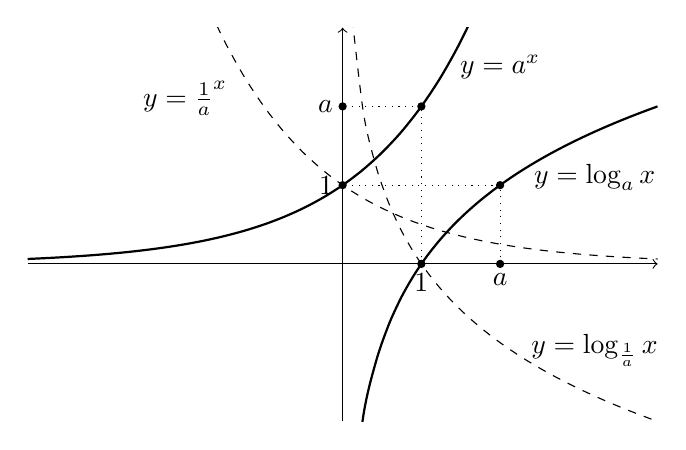
\begin{tikzpicture}[x=1.0cm,y=1.0cm]
      \clip(-4,-2) rectangle (4,3);
    	\draw[->] (-4,0) -- (4,0);
      \draw[->] (0,-2) -- (0,3);
      % y = (3/5)*x + 1/5
      \draw[dotted] (1,0) -- (1,2) -- (0,2);
      \draw[dotted] (2,0) -- (2,1) -- (0,1);
%      \node[right] at (1.75,2.5){$x=-\frac b {2a}$};
      \draw[domain=-2.0:4.0,smooth,variable=\x,dashed] plot
        ({\x}, {pow(2,-\x)});
      \draw[domain=0.1:4.0,smooth,variable=\x,dashed] plot
        ({\x}, {-ln(\x) / ln(2)});
      \draw[domain=-4.0:2.0,smooth,variable=\x,thick] plot
        ({\x}, {pow(2,\x)});
      \node at (2,2.5) {$y=a^x$};
      \node at (-2,2.1) {$y=\enclose{\frac 1 a}^x$};
      \fill (0,1.0) node[left]{\!\!$1$} circle[radius=1.5pt];
      \draw[domain=0.1:4.0,smooth,variable=\x,thick] plot
        ({\x}, {ln(\x) / ln(2)});
      \node at (3.2,1.1) {$y=\log_a x$};
      \node at (3.2,-1.1) {$y=\log_{\frac 1 a} x$};
      \fill (1,0) node[below]{$1$} circle[radius=1.5pt];
      \fill (0,2) node[left]{$a$} circle[radius=1.5pt];
      \fill (2,0) node[below]{$a$} circle[radius=1.5pt];
      \fill (2,1) circle[radius=1.5pt];
      \fill (1,2) circle[radius=1.5pt];
    \end{tikzpicture}
  \end{center}
  \caption{Il grafico della funzione esponenziale e logaritmo 
  in base $a>1$ e $\frac 1 a < 1$ ($a=2$ in figura).}
  \label{fig:esponenziale_logaritmo}
\end{figure}




%
\subsection{logaritmo}
%
%
%

\label{sec:logaritmo}
\index{logaritmo}%

Il teorema di isomorfismo ci dice che fissato $a\in \RR_+$, $a\neq 1$ 
la funzione $\phi_a\colon \RR\to\RR_+$ definita nel paragrafo 
precedente ($\phi_a(x)=a^x$) è bigettiva.
La funzione inversa si chiama \emph{logaritmo in base $a$}
e si denota con $\log_a\colon \RR_+ \to \RR$.

Grazie alle proprietà della funzione esponenziale, già dimostrate
nel teorema~\ref{th:esponenziale} possiamo ottenere 
le proprietà del logaritmo.

\begin{theorem}[proprietà del logaritmo]
Per ogni $a>1$
esiste una unica funzione $\log_a\colon \RR_+\to \RR$ 
tale che 
\begin{enumerate}
  \item $\log_a(a) = 1$;
  \item $\log_a(x\cdot y) =\log_a x + \log_a y$;
  \item $\log_a x \ge 0$ se $x\ge 1$. 
\end{enumerate}
Se $0<a<1$ 
esiste una unica funzione $\log_a$ con le stesse proprietà 
salvo che $\log_a x \le 0$ se $x\ge 1$.

La funzione $\log_a$ viene chiamata \emph{logaritmo in base $a$}
ed ha inoltre le seguenti proprietà valide 
per ogni $a>0$, $a\neq 1$, $x,y\in \RR$, $b>0$, $c>0$, $c\neq 1$:
\begin{enumerate}
  \item $\log_a x = y$ se e solo se $a^y = x$;
  \item $\log_a 1 = 0$;
  \item $\log_a (b^x) = x\log_a b$;
  \item $\log_a x = \frac{\log_c x}{\log_c a}$.
\end{enumerate}
\end{theorem}

\subsection{potenze con esponente reale}

Nel capitolo~\ref{sec:potenza} abbiamo definito 
la funzione potenza $x^n$ con base $x\in \RR$ 
ed esponente $n\in \NN$. 
Invertendo la fuzione $x^n$ 
(solo per $x\ge 0$ quando $n$ è pari e positivo, per ogni $x\in \RR$ se 
$n$ è dispari) abbiamo definito la radice $n$-esima 
$\sqrt[n]{x}$.
Nel capitolo~\ref{sec:esponenziale} abbiamo 
definito la funzione esponenziale $a^x$ con 
base $a\in \RR_+$ ed esponente $x\in \RR$.
La funzione inversa dell'esponenziale 
è il logaritmo $\log_a x$ definito per $x>0$.

Formalmente abbiamo quindi due diverse definizioni 
dell'operazione \emph{potenza} $a^b$ quando $a>0$ 
e $b\in \NN$ ma, ovviamente, queste due definizioni 
coincidono in quanto il teorema di isomorfismo 
ci garantisce che la funzione esponenziale 
$a^x$ coincide con la moltiplicazione ripetuta 
quando $x$ è un numero naturale.
Grazie a questa osservazione possiamo osservare 
che se $x>0$, $p\in \NN$ e $q\in \NN$, $q\neq 0$ si ha 
\begin{equation}
\label{eq:9783023}
  x^{\frac p q} = \sqrt[q]{x^p}, 
  \qquad 
  x^{-\frac p q} = \frac{1}{\sqrt[q]{x^p}}
\end{equation}
in quanto 
\[
  \enclose{x^{\frac p q}}^q = x^p,
  \qquad
  x^{-y} = \frac{1}{x^y}.
\]
Se ripercorriamo la dimostrazione del teorema di isomorfismo 
usando in arrivo il gruppo additivo (è così che abbiamo 
definito la funzione esponenziale) ci accorgiamo 
che la funzione $a^x$ viene dapprima definita sugli $x$
naturali come moltiplicazione ripetuta, 
poi sugli $x$ razionali 
positivi tramite la radice $n$-esima e poi sugli 
$x$ negativi passando al reciproco.

Senz'altro potrà essere utile definire 
$a^{-n} = \frac 1 {a^n}$ avendo quindi una definizione 
di potenza $a^n$ valida per ogni $a$ se $n\in \NN$ 
e per ogni $a\neq 0$ se $n\in \ZZ$.
In alcuni testi si va oltre e si considera $a^b$ 
definito anche quando $a<0$ e $b$ è razionale
utilizzando il lato destro delle equazioni 
in~\eqref{eq:9783023}.
Ognuno può scegliere le definizioni che preferisce 
ed è bene ricordare che le definizioni si scelgono, 
non si dimostrano. 
E' però anche bene sapere che certe definizioni 
possono essere fuorvianti.

Ci sono buoni motivi per pensare che la funzione 
esponenziale $a^x$ ($a>0$) e la funzione potenza $x^n$ 
$n\in \NN$ siano funzioni sostanzialmente diverse.
Si noti ad esempio che le regole delle potenze sono 
soddisfatte da entrambe le definizioni, separatamente, 
ma se mescoliamo le due definizioni le proprietà 
possono cadere. Ad esempio:
\[
  \enclose{(-2)^6}^{\frac 1 2} 
  \neq \enclose{-2}^{6\cdot \frac 1 2}.
\]

Anche il fatto che abbiamo definito $0^0=1$ andrebbe 
interpretato nel senso che lo $0$ all'esponente 
è un numero naturale, non un numero reale:
La funzione esponenziale $a^x$ è definita 
solo per $a>0$ mentre la funzione $x^n$ è definita anche 
per $x=0$ ma solo per $n\in \NN$.


% \begin{figure}
%   \begin{center}
%     \begin{tikzpicture}[x=1.0cm,y=1.0cm]
%       \clip(-3,-2) rectangle (4,3);
%     	\draw[->] (-3,0) -- (4,0);
%       \draw[->] (0,-2) -- (0,3);
%       \draw[dotted] (1,0) -- (1,1) -- (0,1);
%       % \draw[dotted] (2,0) -- (2,1) -- (0,1);
%       \draw[domain=0.5:4,samples=50,variable=\x,thick,dashed] plot
%         ({\x}, {1/(\x*\x))});
%       \draw[domain=-3:-0.5,samples=50,variable=\x,thick,dashed] plot
%         ({\x}, {1/(\x*\x))});
%       \draw[domain=0.2:4,samples=50,variable=\x,dashed,color=gray] plot
%         ({\x}, {1/(\x))});
%       \draw[domain=-3:-0.5,samples=50,variable=\x,dashed,color=gray] plot
%         ({\x}, {1/(\x))});
%       \draw[domain=-2.0:2.0,smooth,variable=\x,thick,color=gray] plot
%         ({\x}, {\x*\x*\x)});
%       \draw[domain=-3.1:4.0,samples=200,variable=\x,color=gray] plot
%         ({\x}, {pow(abs(\x),1/3)*\x / abs(\x)});
%       \draw[domain=-3.0:3.0,smooth,variable=\x,thick] plot
%         ({\x}, {\x*\x});
%       \draw[domain=0.0:4.0,samples=200,variable=\x] plot
%       ({\x}, {pow(\x,1/2)});
%       \node at (-2.0,1.8) {$y=x^2$};
%       \node at (3,2) {$y=\sqrt{x}$};
%       \node[color=gray] at (-1.7,-1.8) {$y=x^{3}$};
%       \node[color=gray] at (-2.0,-1) {$y=\sqrt[3]{x}$};
%       \node[color=gray] at (-1.7,-0.3) {$y=\frac 1 x$};
%       \node at (-2.5,0.6) {$y=\frac 1 {x^2}$};
%       \fill (1,0) node[below]{$1$} circle[radius=1.5pt];
%       \fill (0,1) node[left]{$1$} circle[radius=1.5pt];
%     \end{tikzpicture}
%   \end{center}
%   \caption{Grafici tipici di potenze e radici.}
%   \label{fig:potenza_radice}
% \end{figure}


\subsection{equazioni e disequazioni}

Un problema matematico molto comune è quello di dover risolvere 
equazioni e disequazioni del tipo:
\begin{equation}\label{eq:573197}
  f(x) = b, \quad f(x) \ge b, \quad f(x) > b, 
  \quad f(x) \le b, \quad f(x) < b
\end{equation}
dove $f\colon A \subset \RR \to\RR$ è una funzione data e 
$b\in \RR$ è fissato.

Quando $f$ è strettamente crescente e $b\in f(A)$ 
la soluzione può essere 
scritta banalmente: 
ovviamente deve essere $x\in A$
e ogni equazione o disequazione in~\eqref{eq:573197}
avrà la corrispondente soluzione:
\[
  x= f^{-1}(b), \quad x \ge f^{-1}(b), \quad x>f^{-1}(b),
  \quad x \le f^{-1}(b), \quad x < f^{-1}(b).
\]
Se la funzione fosse strettamente decrescente 
si può procedere allo stesso modo, ma le disuguaglianze si invertono.
Se la funzione fosse strettamente crescente su alcuni intervalli 
e strettamente decrescente su altri si potranno separare i diversi 
casi e si otterranno più soluzioni espresse da uguaglianze
o disuguaglianze.

\begin{example}
  Si risolva la disequazione 
  \[
   \log_2\Enclose{\sqrt[3]{(x+1)^4-3}-2} \le 3. 
  \]
\end{example}%
\begin{proof}[Svolgimento.]
La funzione logaritmo è strettamente crescente ed è definita 
quando l'argomento è positivo. 
Dunque la disequazione data 
è equivalente al sistema di disequazioni:
\[
0 < \sqrt[3]{(x+1)^4 - 3} - 2 \le 8.  
\]
Possiamo sommare $2$ per ottenere 
\[
  2 < \sqrt[3]{(x+1)^4 - 3} \le 10.  
\]
La funzione radice cubica è strettamente crescente 
su tutto $\RR$ quindi possiamo invertirla elevando 
tutto al cubo:
\[
 8 < (x+1)^4 - 3 \le 1000.
\]
Sommiamo $3$:
\[
11 < (x+1)^4 \le 1003.  
\]
L'elevamento alla quarta potenza è strettamente crescente 
solo quando l'argomento è positivo, ed è una funzione pari.
Possiamo quindi affermare che le nostre disequazioni sono 
equivalenti all'unione delle soluzioni di due sistemi:
\[
  \sqrt[4]{11} < x+1 \le \sqrt[4]{1003}
  \qquad\text{o}\qquad 
  -\sqrt[4]{1003} \le x+1 < -\sqrt[4]{11}.
\]
Sottraendo $1$ otteniamo infine 
\[
  \sqrt[4]{11} -1 < x \le \sqrt[4]{1003} - 1
  \qquad\text{o}\qquad 
  -\sqrt[4]{1003} -1 \le x < -\sqrt[4]{11} -1.
\]
In definitiva l'insieme delle soluzioni è 
\[
\left[-\sqrt[4]{1003} - 1, -\sqrt[4]{11}-1\right)
\cup \left(\sqrt[4]{11}-1 , \sqrt[4]{1003} -1\right].  
\]
\end{proof}

Nell'esempio precedente la funzione 
$f(x) = \log_2\Enclose{\sqrt[3]{(x+1)^4-3}-2}$
è ottenuta mediante composizione di funzioni elementari:
\begin{align*}
f &= (x\mapsto \log_2 x)\circ(x\mapsto x-2)\circ (x \mapsto \sqrt[3]{x})\\
  &\quad \circ (x \mapsto x-3) \circ (x\mapsto x^4) \circ (x\mapsto x+1).
\end{align*}
Negli intervalli in cui tutte queste funzioni sono invertibili 
la funzione inversa si ottiene componendo, in ordine opposto,
tutte le inverse:
\begin{align*}
  f^{-1} &= (x\mapsto x-1) \circ (x\mapsto \sqrt[4]{x}) \circ (x \mapsto x+3) \\
    &\quad \circ (x \mapsto x^3) \circ (x \mapsto x+2) \circ (x\mapsto 2^x).
\end{align*}
In effetti il caposaldo $\sqrt[4]{1003}-1$ è proprio tale 
funzione valutata in $b=3$.

Il metodo precedente è puramente algebrico e 
si applica alle equazioni 
come la~\eqref{eq:573197} dove la variabile $x$ 
compare una sola volta e dove la funzione $f$ si esprime 
come composizione di funzioni elementari di cui sappiamo 
scrivere la funzione inversa. 

Ben diverso è il caso in cui nell'equazione la variabile $x$ 
compare più di una volta.
In alcuni casi, come ad esempio,
\[
  x^2 > 2x - 1  
\]
queste equazioni 
possono essere ricondotte al caso precedente tramite 
opportune manipolazioni algebriche.
Il caso delle equazioni quadratiche lo abbiamo 
fatto nel paragrafo precedente utilizzato il completamento 
del quadrato: $x^2-2x = (x-1)^2-1$. 
In altri casi, come ad esempio l'equazione
\[
  2^x = x^2
\]  
le manipolazioni algebriche non sono utili.
Nel capitolo sul calcolo differenziale svilupperemo degli strumenti 
che ci permetteranno di determinare l'andamento di molte di queste 
di funzioni. 
Nel capitolo sulle successioni svilupperemo invece gli strumenti 
che ci permetteranno di determinare le soluzioni mediante 
algoritmi di approssimazione.
Questi strumenti presuppongono il concetto 
di limite e continuità: è sostanzialmente questo che identifica 
la materia chiamata analisi matematica.

\section{polinomi}
\label{ch:polinomi}

Il concetto di ``polinomio'' è una astrazione che non risulta facile esplicitare formalmente.
Nel capitolo~\ref{ch:edo} ci sarà molto utile applicare un polinomio ad un operatore 
differenziale e dunque ci teniamo ora a rendere molto chiaro cosa intendiamo per polinomio.
In particolare distingueremo tre concetti che spesso vengono sovrapposti: 
\emph{espressione polinomiale}, \emph{polinomio} e \emph{funzione polinomiale}.

Se $A$ è un anello abeliano con unità 
(definizione~\ref{def:anello}, 
ad esempio $A=\ZZ$, $A=\QQ$, $A=\RR$ o $A=\CC$)
possiamo considerare tutte le espressioni
(formalmente: alberi di valutazione)
che possono essere costruite utilizzando le operazioni
di addizione e moltiplicazione che coinvolgono coefficienti presi da $A$
e una variabile che possiamo chiamare $x$ 
(e più in generale è possibile considerare polinomi in più variabili).
Queste espressioni verranno chiamate \emph{espressioni polinomiali}%
\mymargin{espressioni polinomiali}%
\index{espressioni!polinomiali} su $A$
(o a coefficienti in $A$) nella variabile $x$. 
Un esempio di espressione polinomiale
è riportato in Figura~\ref{fig:49389}.
\begin{figure}
\begin{center}
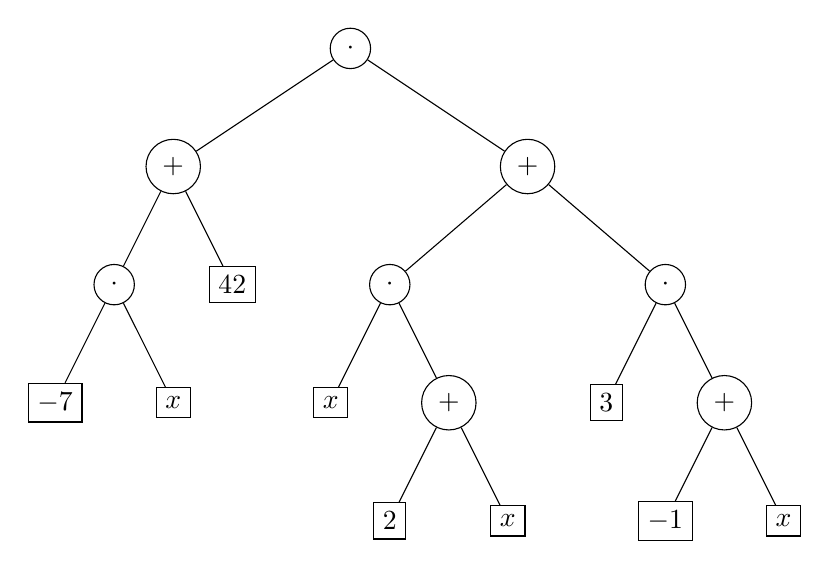
\begin{tikzpicture}
\node [circle,draw] {$\cdot$}
  child {
    node [circle,draw,xshift=-15mm] {$+$}
    child {
      node [circle,draw] {$\cdot$}
      child {node [draw]{$-7$}}
      child {node [draw]{$x$}}
    }
    child {node [draw] {$42$}}
  }
  child {
    node [circle,draw,xshift=15mm] (M) {$+$}
    child {
      node [circle,draw,xshift=-10mm]{$\cdot$}
      child {node [draw]{$x$}}
      child {
        node [circle,draw]{$+$}
        child {node [draw] {$2$}}
        child {node [draw] {$x$}}
        }
      }
    child {
      node [circle,draw,xshift=10mm]{$\cdot$}
      child {node [draw] {$3$}}
      child {
        node [circle,draw] {$+$}
        child {node [draw] {$-1$}}
        child {node [draw] {$x$}}
        }
    }
  };
\end{tikzpicture}
\end{center}
\caption{Il polinomio $P = \enclose{(-7)\cdot x + 42}\cdot(x\cdot (2+x) + 3\cdot(-1+x))$
rappresentato come albero di valutazione.}
\label{fig:49389}%
\end{figure}
Le espressioni polinomiali possono essere sommate e moltiplicate tra loro 
per ottenere nuove espressioni. 
Come comoda notazione si utilizzano le potenze intere per 
denotare un prodotto ripetuto $n$ volte: $x^n = x\cdots x$.

Diremo che due espressioni sono \emph{equivalenti} se è possibile trasformare 
una nell'altra utilizzando le proprietà valide negli anelli abeliani: 
proprietà associativa 
e commutativa per somma e prodotto, proprietà distributiva, elementi 
neutri $1\cdot x = x$, $0 + x = x$.
Inoltre se un ramo dell'espressione non contiene la variabile $x$ è possibile valutare 
(nell'anello $A$) le operazioni e sostituire l'intero ramo con il 
risultato di tali operazioni (e viceversa).

In particolare se abbiamo una qualunque espressione possiamo sviluppare tutti i prodotti
mediante la proprietà distributiva e poi riassociare i termini 
con le stesse potenze di $x$, ad esempio:
\begin{align*}
P &= \enclose{(-7)\cdot x+42}\cdot(x\cdot (2 + x)
+ 3\cdot(-1+x))\\
&= \enclose{(-7)\cdot x + 42}\cdot (2x+x^2-3+3x) \\
% (42-7x)  *  (-3 + 5x + x^2)
&= 126 + 231 x + 7 x^2 - 7 x^3
\end{align*}
In generale si otterrà una espressione polinomiale che diremo 
essere in \emph{forma canonica}:
\[
  P = a_0 + a_1 x + a_2 x^2 + \dots + a_n x^n
       = \sum_{k=0}^n a_k x^k.
\]
Dunque ogni espressione polinomiale è equivalente ad una 
espressione polinomiale in forma canonica. 

Se due espressioni polinomiali sono equivalenti 
diremo che rappresentano lo stesso \emph{polinomio}%
\mymargin{polinomio}%
\index{polinomio}.
Se $A$ è un anello denoteremo con 
$A[x]$ \index{$\KK[x]$}\index{$A[x]$}%
l'insieme di tutti i polinomi con coefficienti in $A$ e variabile $x$. 
Formalmente $A[x]$ è il quoziente dell'insieme 
di tutte le espressioni polinomiali rispetto alla relazione di equivalenza
che abbiamo appena definito. 
Possiamo fare la somma e il prodotto di polinomi e queste operazioni 
rendono $A[x]$ anch'esso un anello.

Più esplicitamente se $P$ e $Q$ sono polinomi in forma canonica
\[
  P = \sum_{k=0}^n a_k x^k, \qquad Q = \sum_{k=0}^m b_k x^k
\]
si avrà:
\[
  P + Q = \sum_{k=0}^{N} (a_k+b_k) \cdot x^k
\]
dove $N$ è il più grande tra $n$ e $m$ e si intende che $a_k=0$ per $k>n$ e 
$b_k=0$ per $k>m$.
Se $t\in A$ avremo:
\[
  t P = \sum_{k=0}^n (ta_k)\cdot x^k.
\]
Per quanto riguarda il prodotto si avrà invece:
\begin{align*}
  P\cdot Q
  &= \enclose{\sum_{k=0}^n a_k x^k}\cdot \enclose{\sum_{j=0}^n b_j x^j}
  = \enclose{\sum_{k=0}^n a_k \enclose{\sum_{j=0}^m b_j x^j} x^k} \\
  &= \enclose{\sum_{k=0}^n \sum_{j=0}^m a_k b_j x^{j+k}}
  = \sum_{s=0}^{m+n} \enclose{\sum_{j=0}^s a_j b_{s-j}} x^s.
\end{align*}

Le formule per la somma e il prodotto dei polinomi in forma canonica 
possono essere applicate ad ognuna delle proprietà di anello per dimostrare
che polinomi equivalenti hanno la stessa forma canonica e che quindi 
due espressioni polinomiali sono equivalenti se e solo se i coefficienti 
della loro forma canonica coincidono.
In pratica i polinomi a coefficienti in $A$ sono 
rappresentati dai coefficienti delle loro forme canoniche che 
non sono altro che sequenze finite:
\begin{align*}
  A[x] 
  &= \{\sum_{k=0}^n a_k x^k\colon a_k\in A, n\in \NN\}\\
  &\approx A^\NN_c 
  = \ENCLOSE{\vec a \in A^\NN\colon \ENCLOSE{k\in \NN\colon \vec a(k)\neq 0} \text{ è finito}}.  
\end{align*}

Se il polinomio $P$ si scrive in forma canonica
\[
  P = \sum_{k=0}^n a_k x^k
\]
se $n>0$ possiamo supporre che il coefficiente $a_n$ sia diverso da $0$ 
perché altrimenti potremmo rimuovere il termine corrispondente e ridurci 
ad una somma di $n-1$ termini. 
In tal caso diremo che il polinomio $P$ ha \emph{grado}%
\mymargin{grado}%
\index{grado} $n$.
\index{polinomio!grado}%
\index{grado!polinomio}% 
Se $n=0$ diremo anche che il polinomio è costante.
Se $n=0$ e $a_n=0$ diremo che $P$ è il polinomio \emph{nullo}.
I polinomi costanti non nulli hanno grado pari a $0$, mentre il polinomio nullo, 
per convenzione, diremo avere grado $-\infty$ (questa definizione ha senso se si pensa 
al grado di un polinomio come al più piccolo numero per cui tutti i coefficienti di
indice maggiore a lui sono nulli).

Finora abbiamo definito il polinomio come una classe di equivalenza di 
espressioni polinomiali. 
Se prendiamo una espressione $P$ e al posto della variabile $x$ 
mettiamo un elemento $a$ dell'anello $A$ (o di qualunque anello che estende 
$A$) allora possiamo valutare tutte le operazioni (somme e prodotti) ed 
ottenere un risultato nell'anello scelto: il risultato 
ottenuto si indica con $P(a)$ (stessa notazione utilizzata per le funzioni).
Se $P$ è un polinomio nella variabile $x$ la funzione $x\mapsto P(x)$ 
può essere chiamata \emph{funzione polinomiale}%
\mymargin{funzione polinomiale}%
\index{funzione!polinomiale} e si indica usualmente 
con con lo stesso nome $P$ dato al polinomio. Sarà il contesto a dirci 
se con $P$ si intende il polinomio (l'espressione) o la funzione.

Come già anticipato è utile tenere separato il concetto di polinomio da quello di 
funzione polinomiale in quanto lo stesso polinomio può essere valutato su diversi 
anelli (ad esempio nel corso di geometria si potrà sostituire
la variabile $x$ di un polinomio con una matrice, 
e nell'ultimo capitolo di questi appunti 
sostituiremo la $x$ con un operatore differenziale).

Proseguiremo con la trattazione dei polinomi 
nel capitolo~\ref{ch:ancora_polinomi}.

\subsection{coefficienti binomiali}
\label{ch:binomiale}

Capiterà spesso di imbattersi in alcuni polinomi particolari, che vengono 
a volte chiamati \emph{prodotti notevoli}%
\mymargin{prodotti notevoli}%
\index{prodotto!notevole}. 
Di fondamentale iportanza quelli di grado 2:
\[
  (x+1)\cdot(x-1) = x^2-1, \qquad (x+1)^2 = x^2+2x + 1.
\]
Ma anche quelli di grado $n$:
\[
  (x-1)\cdot \sum_{k=0}^{n-1} x^k
  = \sum_{k=0}^{n-1} x^{k+1} - \sum_{k=0}^n x^k = x^n - 1
\]
e, mettendo $-x$ al posto di $x$ e cambiando di segno:
\[
  (x+1)\cdot \sum_{k=0}^{n-1} (-1)^k x^k
  = 1 + (-1)^n x^n.
\]

Le potenze del binomio $x+1$ sono decisamente rilevanti. 
Se scriviamo il polinomio $(x+1)^n$ in forma canonica:
\[
  (x+1)^n = \sum_{k=0}^n a_k x^k  
\]
saremmo interessati a calcolare il valore
dei coefficienti $a_k$. 
Innanzitutto gli diamo un nome: questi coefficienti vengono chiamati 
\emph{coefficienti binomiali}%
\mymargin{coefficienti binomiali}%
\index{coefficienti binomiali}
\index{binomio!coefficienti}%
e si denotano nel modo seguente:%
\mynote{%
I coefficienti binomiali nell'ambito del calcolo combinatorio 
vengono anche chiamati \emph{combinazioni}
e denotati con il simbolo $C_{n,k} = {n \choose k}$.
La coincidenza tra le combinazioni e i coefficienti binomiali 
è espressa nel teorema~\ref{th:combinatoria}.
}%
\[
    a_k = {n \choose k}.
\]

Non è difficile convincersi che se sviluppiamo il binomio $(x+y)^n$
si ottengono gli stessi coefficienti dunque
in generale vale la seguente formula per la \emph{potenza del binomio}%
\mymargin{potenza del binomio}%
\index{potenza!del binomio}:
\index{binomio!potenza}% 
\begin{equation*}
  (x+y)^n = \sum_{k=0}^n {n \choose k} x^k y^{n-k}. 
\end{equation*}

Per determinare il valore effettivo dei coefficienti 
binomiali si utilizza usualmente il seguente.
  
\begin{theorem}[triangolo di Tartaglia]
\mymark{*}%
\label{th:tartaglia}%
Per ogni $n\in \NN$ e $k \in \NN$ con $1 \le k \le n$ si ha
\[
  {n+1 \choose k} =
      {n \choose k-1} + {n \choose k}
\]
mentre
\[
  {n+1 \choose 0} = 1 = {n+1 \choose n+1}
\]
\end{theorem}
  %
  \begin{proof}
  Infatti si ha 
  \begin{align*}
    \sum_{k=0}^{n+1} {n+1 \choose k} x^k
    &= (1+x)^{n+1} 
    = (1+x)\cdot \sum_{k=0}^n {n \choose k} x^k \\
    &= \sum_{k=0}^n {n\choose k} x^k 
    + \sum_{k=0}^n {n\choose k} x^{k+1}\\
    &= \sum_{k=0}^n {n\choose k} x^k 
    + \sum_{k=1}^{n+1} {n\choose k-1} x^{k}\\
    &= {n\choose 0} x^0 
      + \sum_{k=1}^n \Enclose{{n\choose k} + {n\choose k-1}} x^k
      + {n \choose n} x^{n+1}.
    \end{align*}
  Per l'unicità della forma canonica dei polinomi 
  i coefficienti corrispondenti devono essere uguali e quindi 
  troviamo
  \[
  {n+1 \choose 0} = {n \choose 0}, \qquad 
  {n+1 \choose k} = {n \choose k} + {n \choose k-1}, \qquad 
  {n+1 \choose n+1} = {n \choose n}.
  \]

  Si può facilmente verificare che  ${0 \choose 0} = 1$ 
  e questo conclude la dimostrazione.
  \end{proof}
  
  In base al teorema precedente i coefficienti binomiali si possono
  elencare come nella tabella~\ref{tab:binomiali}:
  ogni riga inizia e finisce con il numero $1$
  e ogni termine intermedio coincide con la somma dei
  due termini nella riga precedente sopra e
  a sinistra del numero considerato.
  
  \begin{table}
  \begin{tabular}{c|ccccccccc}
  $\displaystyle{n \choose k}$& 0 & 1 & 2 & 3 & 4 & 5 & 6 & $k$ &\\ \hline
    0 & 1 &   &   &   &   &   &   & &\\
    1 & 1 & 1 &   &   &   &   &   & &\\
    2 & 1 & 2 & 1 &   &   &   &   & &\\
    3 & 1 & 3 & 3 & 1 &   &   &   & &\\
    4 & 1 & 4 & 6 & 4 & 1 &   &   & &\\
    5 & 1 & 5 & 10& 10& 5 & 1 &   & &\\
    6 & 1 & 6 & 15& 20& 15& 6 & 1 & &\\
  $n$ &$\vdots$&&   &   &   &   &   & $\ddots$ &
  \end{tabular}
  \caption{Il triangolo di Tartaglia (o di Pascal):
  ogni numero è la somma dei due numeri che si trovano 
  nella riga precedente sopra e immediatamente a sinistra.}
  \label{tab:binomiali}
  \end{table}
  
  \begin{theorem}[formula per i coefficienti binomiali]
  \mymark{***}%
  Se $n\in \NN$ e $k\in \NN$, $k\le n$
  si ha 
  \[
  {n \choose k}  
  = \frac{n!}{k!(n-k)!}.  
  \]
  \end{theorem}
  %
  \begin{proof}
  Lo dimostriamo per induzione su $n$.
  Per $n=0$ sappiamo che ${0 \choose 0} = 1$ che 
  è ugule a $\frac{0!}{0!0!}$.
  Utilizziamo il teorema~\ref{th:tartaglia}.
  Se $k=0$ o $k=n$ sappiamo che ${n \choose k}=1$ che coincide 
  con la formula enunciata. 
  Per gli altri casi, supponendo per induzione che la formula sia 
  vera per un certo $n\in \NN$ si ha: 
  \begin{align*}
   {n+1 \choose k} 
   &= {n \choose k} + {n \choose k-1}
   =  \frac{n!}{k!(n-k)!} + \frac{n!}{(k-1)!(n-k+1)!} \\
   &= \frac{n!(n-k+1) + n! k}{k!(n-k+1)!}
   = \frac{n!(n+1)}{k!(n+1-k)!} \\
   &= \frac{(n+1)!}{k!(n+1-k)!}
  \end{align*}
  che è quanto dovevamo dimostrare.
\end{proof}

Si osservi che risulta, per ogni $n\in \NN$:
\[
  {n \choose 1} = {n \choose n-1} = n.
\]
  
\begin{exercise}
  Provare che
  \[
   \sum_{k=0}^n {n \choose k} = 2^n.
  \]
\end{exercise}  


\subsection{scomposizione dei polinomi}

\begin{theorem}[divisione di Euclide]
  \label{th:divisione_polinomi}%
  \index{divisione tra polinomi}%
  \index{polinomio!divisione}%
  \index{polinomio!algoritmo di Euclide}%
  \index{Euclide!algoritmo di divisione}%
  \index{algoritmo!di Euclide}%
  Se $\KK$ è un campo,
  dati due polinomi $P$ e $S$ in $\KK[x]$ con $S\neq 0$ è possibile
  trovare, in modo unico, due polinomi $Q$ (quoziente)
  e $R$ (resto) in $\KK[x]$ con $\deg R < \deg S$
  tali che:
  \[
    P = Q \cdot S + R.
  \]
  \end{theorem}
  %
  \begin{proof}
  \emph{Passo 1:} supponiamo che sia $\deg P < \deg S$.
  In questo caso basta prendere $Q=0$ e $R=P$.
  
  \emph{Passo 2:} supponiamo che sia $\deg P \ge \deg S$.
  Poniamo $N=\deg P$ e $M=\deg S$.
  Sia $a_N\neq 0$ il coefficiente del termine di grado massimo
  di $P$ e $b_M\neq 0$ il coefficiente di grado massimo
  del polinomio $S$.
  E' allora facile verificare che il polinomio
  \[
  \frac{a_N}{b_M} \cdot x^{N-M}\cdot S
  \]
  ha lo stesso grado di $P$ e il suo coefficiente di grado
  massimo è uguale ad $a_N$ in quanto è il prodotto di
  $a_N/b_M$ per $b_M$.
  Dunque il polinomio
  \[
   P_1 = P - \frac{a_N}{b_M} \cdot x^{N-M}\cdot S
  \]
  ha grado strettamente inferiore a $P$.
  Possiamo ora supporre, mediante un ragionamento induttivo
  su $\deg P - \deg S$
  che per il polinomio $P_1$ il risultato del teorema sia
  valido cioè
  che esistano, dei polinomio $Q_1$ e $R$
  con $\deg R < \deg S$ tali che
  \[
    P_1 = Q_1 \cdot S + R.
  \]
  Il caso base del ragionamento induttivo,
  $\deg P = \deg S$, è garantito dal passo 1.
  Avremo allora:
  \begin{align*}
    P &= P_1 + \frac{a_N}{b_M} x^{N-M}\cdot S\\
      &= Q_1 \cdot S + R_1 + \frac{a_N}{b_M} x^{N-M}\cdot S\\
      &= (\frac{a_N}{b_M} x^{N-M} + Q_1) \cdot S + R_1.
  \end{align*}
  Posto quindi
  \[
   Q = \frac{a_N}{b_N} x^{N-M} + Q_1
  \]
  il risultato è dimostrato.
  
  \emph{Passo 3:} dimostriamo che $Q$ e $R$ sono unici. Se infatti avvessimo 
  \[
    P = Q_1 S + R_1 = Q_2 S + R_2   
  \]
  con $\deg R_1<\deg S$ e $\deg R_2 < \deg S$ si avrebbe 
  \[
  (Q_2 - Q_1) S = R_1 - R_2.    
  \]
  Se fosse $Q_2 \neq Q_1$ il polinomio al lato sinistro avrebbe grado non inferiore al grado di 
  $S$ mentre il lato destro ha certamente grado minore di $S$.
  Dunque $Q_2=Q_1$ ma allora il lato sinistro è nullo e quindi anche il lato destro deve 
  esserlo: $R_2=R_1$.
  \end{proof}
  
  La dimostrazione del teorema precedente fornisce anche un
  algoritmo, chiamato \emph{algoritmo di Euclide},
  per eseguire la divisione (con resto) tra polinomi.
  Lo sperimentiamo nel seguente esercizio.
  
  \begin{exercise}
  Sia $P = x^4-3 x^2 + 2x + 1$ e $S = x^2-1$.
  Eseguire la divisione con resto cioè:
  trovare $Q$ ed $R$ con $\deg R < \deg S$ tali che
  \[
  P = Q \cdot S + R.
  \]
  \end{exercise}
  %
  \begin{proof}[Svolgimento.]
  Il rapporto tra i termini di grado massimo di
  $P$ e $S$ è $x^4/x^2 = x^2$.
  Dunque consideriamo come primo monomio $x^2$.
  Si ha
  \begin{align*}
    P_1
    &= P - x^2 \cdot S
    = x^4-3x^2+2x+1 - x^4+x^2 \\
    &= -2x^2+2x+1.
  \end{align*}
  Ripetiamo il procedimento con $P_1$ al posto di $P$.
  Il rapporto tra i termini di grado massimo di $P_1$ e $S$
  è il monomio $-2$. Si ha
  \[
    P_2 = P_1 - (-2) S = -2x^2 + 2x + 1 + 2x^2 - 2 = 2x -1.
  \]
  Visto che $\deg P_2 < \deg S$ la divisione termina e
  si pone $R = 2x-1$.
  Si ha quindi $Q = x^2 - 2$ (la somma dei monomi trovati)
  e risulta:
  \[
    P = (x^2 - 2)\cdot S + 2x -1.
  \]
  \end{proof}
  
  \begin{theorem}[Ruffini]
  \label{th:Ruffini}%
  \index{teorema!di Ruffini}%
  \index{Ruffini}%
  Sia $P\in \KK[x]$ un polinomio non nullo.
  Se $x_0 \in \KK$ è tale che $P(x_0)=0$
  allora esiste un polinomio $Q$ con $\deg Q = (\deg P) - 1$
  tale che
  \[
    P = (x-x_0)\cdot Q.
  \]
  \end{theorem}
  %
  \begin{proof}
  In base al teorema precedente si può fare la divisione tra
  $P$ e $S = x - x_0$ per ottenere un polinomio $Q$ e un resto
  $R$ con $\deg R < 1$ tali che
  \[
    P = (x-x_0)\cdot Q + R.
  \]
  Siccome $\deg R < 1$ si ha in effetti che $R=c\in \KK$
  è un polinomio costante e dunque
  \[
    P = (x-x_0) \cdot Q + c
  \]
  ma valutando $P$ in $x=x_0$ si scopre che
  \[
   P(x_0) = 0\cdot Q(x_0) + c = c
  \]
  dunque $c=P(x_0) = 0$.
  \end{proof}
  
  Possiamo ora chiederci se polinomi diversi corrispondono
  a funzioni polinomiali diverse.
  In generale questo non è vero, se ad esempio prendessimo
  come campo $\KK=\ZZ_2 = \ENCLOSE{0,1}$, un campo finito
  in cui poniamo $1+1=0$ scopriremmo che la funzione polinomiale
  $P(x) = x^2+x$ è identicamente nulla in quanto $0^2+0=0$
  e $1^2+1=1+1=0$ in questo campo.
  Ma nei casi che interessano a noi $\KK=\RR$ o $\KK=\CC$
  questo problema non si presenta e si potrà quindi identificare
  ogni polinomio con la corrispondente funzione polinomiale.
  Per avere questa garanzia ci servono i seguenti risultati.
  
  \begin{theorem}[principio di annullamento dei polinomi]
  \label{th:annullamento_polinomi}%
  \index{principio!di annullamento dei polinomi}%
  Sia $P\in \KK[x]$ un polinomio non nullo di grado $n$.
  Allora la funzione polinomiale associata a $P$
  si annulla in al più $n$ punti distinti di $\KK$.
  
  In particolare se un polinomio si annulla in infiniti
  punti distinti allora tale polinomio è certamente nullo.
  \end{theorem}
  %
  \begin{proof}
  Dimostriamo per induzione su $n$ che se un polinomio
  $P$ di grado non superiore a $n$ si annulla in $n+1$
  punti distinti $x_1, \dots, x_{n+1}\in \KK$ allora
  $P=0$.
  
  Se $n=0$ il polinomio $P$ è costante ma si annulla
  in un punto e quindi è il polinomio nullo.
  Se $n>0$ per il teorema di Ruffini applicato al
  punto $x_{n+1}$ sappiamo che esise un polinomio $Q$
  di grado inferiore ad $n$ per cui si ha
  \[
    P = (x-x_{n+1}) \cdot Q
  \]
  sostituendo $x=x_k$ con $k\le n$ si ha $x_k-x_{n+1}\neq 0$
  e quindi
  \[
    Q(x_k) = \frac{P(x_k)}{x_k-x_{n+1}} = 0.
  \]
  Dunque $Q$ si annulla nei punti $x_1, \dots, x_n$
  e, per ipotesi induttiva, scopriamo che $Q$ deve
  essere nullo. Di conseguenza anche $P$ è nullo.
  \end{proof}
  
  Se $\KK$ è un insieme infinito (come nei casi $\KK=\RR$ o $\KK=\CC$)
  si trova che
  se a due polinomi $P$, $Q$ corrisponde
  la stessa funzione polinomiale:
  \[
    P(x) = Q(x) \qquad \text{per ogni $x\in \KK$}
  \]
  allora $P$ e $Q$ sono lo stesso polinomio $P=Q$
  in quanto la differenza $P-Q$ si annulla in tutti i punti
  di $\KK$ e qualunque sia il suo grado, se $\KK$ è infinito,
  questo ci dice che $P-Q=0$. 
  
  Questo corollario viene spesso enunciato come segue.
  \begin{theorem}[principio di identità dei polinomi]
    Siano $a_k$ e $b_k$ coefficienti nel campo $\KK=\RR$ o $\KK=\CC$.
    Se per ogni $x\in \KK$ si ha 
    \[
       \sum_{k=1}^n a_k x^k = \sum_{k=1}^m b_k x^k
    \]
    allora $m=n$ e $a_k=b_k$ per ogni $k=0, \dots, n$.
  \end{theorem}
  %
  \begin{proof}
  Facendo la differenza dei due lati dell'uguaglianza si ottiene 
  che una espressione polinomiale si annulla identicamente. 
  Allora per il teorema~\ref{th:annullamento_polinomi} tale espressione 
  rappresenta il polinomio nullo e di conseguenza tutti i coefficienti, 
  che sono dati dalla differenza $a_k-b_k$, devono essere nulli.
  \end{proof}
  
\begin{example}
L'insieme $\ZZ_2={0,1}$ può essere reso un campo 
se si definisce la somma e il prodotto come sui 
numeri naturali prendendo però sempre il resto 
modulo $2$: $0+0=1+1=0$, $0+1=1+0=1$, $0\cdot 0
=1\cdot 0 = 0\cdot 1 = 0$, $1\cdot 1=1$.
Si può verificare che effettivamente $\ZZ_2$ 
è un campo.
Il polinomio $P = x^2+x$ risulta annullarsi sia 
per $x=0$ che per $x=1$, ma non è il polinomio nullo.
\end{example}

\section{i numeri complessi}
%
%
%
\label{sec:complessi}

Dal punto di vista geometrico l'insieme $\CC$ dei \emph{numeri complessi}%
\mymargin{numeri complessi}%
\index{numeri!complessi}
\index{$\CC$}
può essere visto come una rappresentazione cartesiana 
del piano euclideo.
Sul piano fissiamo arbitrarimente un punto $0$ (l'origine) 
e fissiamo, arbitrariamente, una base $e_1$, $e_2$ di vettori ortonormali.
Identifichiamo ogni punto del piano con i corrispondenti vettori
applicati in $0$. La retta generata dal vettore $e_1$ la identifichiamo
con la retta $\RR$ dei numeri reali e quindi poniamo $1=e_1$.
La retta ortogonale generata dal vettore $e_2$ verrà chiamata
retta dei \emph{numeri immaginari} e definiamo $i=e_2$.

Un generico punto $z$ del piano $\CC$ potrà essere scritto in
maniera univoca nella base scelta: $z = x e_1 + y e_2$ ovvero,
per come abbiamo chiamato $e_1$ ed $e_2$:
\[
z = x + i y.
\]
Tale $z$ viene chiamato
\emph{numero complesso} con parte reale $x$ e parte immaginaria $y$.
Questa rappresentazione del numero complesso $z$ viene
chiamata \emph{rappresentazione cartesiana}%
\mymargin{rappresentazione cartesiana}%
\index{rappresentazione!cartesiana} in quanto definisce
il punto $z$ del piano complesso tramite le sue coordinate cartesiane
$x$ e $y$.
I numeri reali sono \emph{immersi} nei complessi, nel senso che se
$x\in \RR$ allora $z= x + i\cdot 0 = x$ è anche un numero complesso.
Il numero complesso $i = 0 + i\cdot 1$ viene chiamata \emph{unità immaginaria}%
\mymargin{unità immaginaria}%
\index{unità!immaginaria}
e i numeri complessi della forma $iy$ sono chiamati \emph{immaginari}.
\index{numeri!immaginari}
\index{immaginario}
Un numero
complesso $z = x+iy$ è quindi una somma tra un numero reale ed un numero
immaginario. Il numero reale $x$ viene chiamato \emph{parte reale}
\index{parte!reale}
di $z$ e
si denota con $x=\Re z$.
\mymargin{$\Re z$}%
\index{$\Re z$}
Il numero reale $y$ viene chiamato
\emph{parte immaginaria}
\index{parte!immaginaria}
di $z$ e si denota con $y=\Im z$
\mymargin{$\Im z$}%
\index{$\Im z$}
(osserviamo che la parte immaginaria di un numero complesso è un numero
reale, non immaginario). Dunque $z= \Re z + i \Im z$.

L'insieme $\CC$, per come
è stato costruito, è uno spazio vettoriale reale di dimensione $2$.
Abbiamo quindi già definite la \emph{addizione}%
\mymargin{addizione}%
\index{addizione}
\index{complessi!addizione}
tra elementi di $\CC$ e la moltiplicazione
tra elementi di $\CC$ ed elementi di $\RR$.
Se $a,b,c,d,t\in \RR$ si ha:
\begin{gather*}
 (a+ib) + (c+id) = (a+c) + i (b+d), \\
 t(a+ib) = ta + itb.
\end{gather*}

Vogliamo estendere la \emph{moltiplicazione}%
\mymargin{moltiplicazione}%
\index{moltiplicazione} a tutte le coppie di numeri complessi.
\index{complessi!moltiplicazione}
Imponendo (arbitrariamente) che valga $i\cdot i = -1$ e che rimanga
valida la proprietà distributiva, si ottiene
questa definizione:
\[
   (a+ib) \cdot (c+id) = (ac-bd) + i(ad+bc).
\]

Si può verificare che questa moltiplicazione estende quella ``scalare'' definita
in precedenza.
E' anche facile verificare che addizione e moltiplicazione soddisfano
le proprietà commutativa associativa e distributiva,
che $0$ è elemento neutro per la addizione, che $1$ è elemento neutro
della moltiplicazione.
Si osservi che se $z=x+iy$ non è nullo, allora
\[
  (x+iy) \cdot \frac{x-iy}{x^2+y^2} = 1.
\]
Significa che ogni $z\neq 0$ ammette inverso moltiplicativo e quindi $\CC$
risulta essere un campo.

Osserviamo che su $\CC$ non si definisce una relazione d'ordine perché
in effetti non è possibile definire un ordine ``compatibile'' con le operazioni
appena definite.%
\mynote{%
Se $\CC$ fosse un campo ordinato per assurdo
si dovrebbe avere,
che $z^2\ge 0$ per ogni $z\in \CC$ (questo è vero in tutti i campi ordinati). 
Ma
allora $-1 =i^2 \ge 0$ cioè $1\le 0$ che è in contraddizione
con la proprietà $0<1$ valida in ogni campo ordinato.
} % marginnote

Su $\CC$ definiamo delle ulteriori operazioni.
Il \emph{coniugato}%
\mymargin{coniugato}%
\index{coniugato}%
\index{complessi!coniugio}
di un numero complesso $z=x+iy$ è il numero
$\bar z = x - iy$. Geometricamente l'operazione di coniugio è una simmetria
rispetto alla retta reale. I numeri reali sono in effetti punti fissi del
coniugio (il coniugato di un numero reale è il numero stesso).
E' un semplice esercizio verificare che il coniugio ``attraversa''
somma e prodotto:
\[
\overline{z+w} = \bar z + \bar w, \qquad
\overline{z\cdot w} = \bar z \cdot \bar w.
\]
Ovviamente risulta $\overline {\bar z} = z$.
E' anche utile osservare che si ha:
\begin{equation}\label{eq:re_im}
  \Re z = \frac{z+\bar z}{2}, \qquad
  \Im z = \frac{z-\bar z}{2i}
\end{equation}
e
\[
z \cdot \bar z = (x+iy)(x-iy) = x^2-i^2y^2 = x^2+y^2.
\]

Possiamo allora definire il
\emph{modulo}%
\mymargin{modulo}%
\index{modulo}%
\index{complessi!modulo}
 di un numero complesso $z=x+iy$
come il numero reale
\[
\abs{z} = \sqrt{z\cdot\bar z} = \sqrt{x^2+y^2}.
\]
Geometricamente tale quantità rappresenta la distanza del punto $z$
dal punto $0$ e quindi la distanza tra due numeri complessi $z$ e
$w$ si potrà rappresentare con $\abs{z-w}$.

Osserviamo che se $z = x \in \RR \subset \CC$ il modulo di $z$ coincide
con il valore assoluto: $\abs{z} = \sqrt{x^2} = \abs{x}$ e per questo
motivo non distinguiamo, nelle notazioni, il modulo dal valore assoluto.
Più in generale risulta per ogni $z\in \CC$ (la verifica è immediata):
\[
  \abs{\Re z} \le \abs{z}, \qquad
  \abs{\Im z} \le \abs{z}.
\]

Possiamo a questo punto trovare una utile formula per calcolare
il reciproco di un numero complesso. Essendo infatti
$z\cdot \bar z = \abs{z}^2$ si osserva che
\[
  \frac{1}{z}
  = \frac{\bar z}{ \bar z \cdot z}
  = \frac{\bar z}{\abs{z}^2}.
\]

\begin{theorem}
Il modulo di un numero complesso soddisfa (come il valore assoluto)
le seguenti proprietà
\begin{enumerate}
\item $\big\lvert\abs{z}\big\rvert = \abs{z}$,
\item $\abs{-z} = \abs{z}$ = $\abs{\bar z}$,
\item $\abs{z\cdot w} = \abs{z}\cdot\abs{w}$.
\item $\abs{z+w} \le \abs{z}+\abs{w}$ (convessità),
\item $\abs{z-w} \le \abs{z-v} + \abs{v-w}$ (disuguaglianza triangolare),
\end{enumerate}
\end{theorem}
%
\begin{proof}
La prima proprietà è ovvia in quanto il valore assoluto di un numero reale
non negativo è il numero stesso.

La seconda proprietà viene immediatamente dalla definizione.

Per la terza proprietà sia $z=x+iy$, $w=a+ib$.
Allora:
\begin{align*}
\abs{z\cdot w}
&= \abs{(x+iy)\cdot(a+ib)}
=\abs{xa - y b+ i(xb + ay)} \\
&= \sqrt{(xa-yb)^2 + (xb+ay)^2}\\
&=\sqrt{x^2 a^2 + y^2b^2 - 2xayb + x^2b^2+a^2y^2+2xbay} \\
&=\sqrt{x^2 a^2 + y^2 b^2 + x^2 b^2 + a^2 y^2}\\
&=\sqrt{x^2(a^2+b^2) + y^2(a^2+b^2)}\\
&=\sqrt{(x^2+y^2)(a^2+b^2)}
=\abs{x+iy} \cdot \abs{a+ib}\\
&=\abs{z}\cdot\abs{w}.
\end{align*}

Per la quarta disuguaglianza osserviamo che si ha
\[
  \abs{z+w}^2 = (z+w)\cdot(\bar z + \bar w)
  = \abs{z}^2 + \abs{w}^2 + z\cdot \bar w + \bar z \cdot w
\]
e visto che
\[
  z\cdot \bar w + \bar z \cdot w
  = z \cdot \bar w + \overline{z \cdot \bar w}
  = 2 \Re(z\bar w)
  \le 2 \abs {z\bar w}
  = 2 \abs{z}\cdot\abs{\bar w}
  = 2 \abs{z}\cdot\abs{w}
\]
otteniamo
\[
 \abs{z+w}^2 \le \abs{z}^2+\abs{w}^2 + 2 \abs{z}\cdot\abs{w}
 =\enclose{\abs z + \abs w}^2
\]
che è equivalente alla disuguaglianza di convessità.

La disuguaglianza triangolare è conseguenza immediata della convessità, infatti
\[
  \abs{z-w} = \abs{(z-v) + (v-w)}
  \le \abs{z-v} + \abs{v-w}.
\]
\end{proof}

\begin{figure}
  \begin{center}
    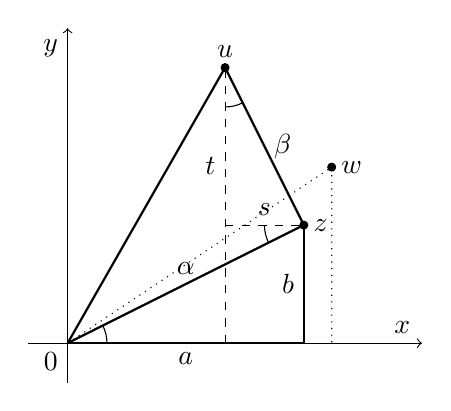
\begin{tikzpicture}[x=0.5cm,y=0.5cm]
    	\draw[->] (-1,0) -- (9,0);
      \draw[->] (0,-1) -- (0,8);
      %
      \draw[dotted] (0,0) -- ({sqrt(45)},{sqrt(20)}) -- ({sqrt(45)},0);
      \draw[fill] ({sqrt(45)},{sqrt(20)}) node[right] {$w$} circle [radius=0.1];
      %
      \draw[thick] (0,0) -- (6,0);
      \draw[thick] (0,0) -- (6,3);
      \draw[thick] (0,0) -- (4,7);
      \draw[thick] (6,0) -- (6,3);
      \draw[thick] (6,3) -- (4,7);
      %
      \draw[dashed] (4,0) -- (4,7);
      \draw[dashed] (4,3) -- (6,3);
      %
      \draw (1,0) arc (0:{atan(1/2)}:1);
      \draw (6,3)+(-1,0) arc (180:{180+atan(1/2)}:1);
      \draw (4,7)+(0,-1) arc (-90:{-90+atan(1/2)}:1);
      %
      \draw[fill] (6,3) node[right] {$z$} circle [radius=0.1];
      \draw[fill] (4,7) node[above] {$u$} circle [radius=0.1];
      %
      \node[below] at (3,0) {$a$};
      \node[left] at (6,1.5) {$b$};
      \node[above] at (3,1.5) {$\alpha$};
      \node[right] at (5,5) {$\beta$};
      \node[above] at (5,3) {$s$};
      \node[left] at (4,4.5) {$t$};
      \node[above] at (8.5,0) {$x$};
      \node[left] at (0,7.5) {$y$};
      \node[below left] at (0,0) {$0$};
    \end{tikzpicture}
  \end{center}
  \caption{Consideriamo i numeri complessi $z=a+ib$ e $w=\alpha+i\beta$
  e supponiamo che sia $\alpha^2 = a^2+b^2$.
  Si consideri il punto $u$ che si ottiene ruotando il punto $w$ dell'angolo
  individuato dal punto $z$. Si avrà allora $u=a-s + i(b+t)$ dove $s$ e $t$
  sono i cateti del triangolo rettangolo con ipotenusa $\beta$.
  Grazie alle proprietà di similitudine dei triangoli si ha
  $\frac{s}{\beta} = \frac{b}{\alpha}$ e $\frac{t}{\beta} = \frac{a}{\alpha}$
  da cui si ottiene quindi $u = a-\frac{b\beta}{\alpha}+i(b+\frac{a\beta}{\alpha})$
  ovvero $\alpha u = (a\alpha - b \beta) + i (b\alpha + a \beta) = z\cdot w$.
  Significa che il numero complesso $z\cdot w$ si trova sulla semiretta
  che individua un angolo che è la somma degli angoli individuati
  dai numeri complessi $z$ e $w$.
  }
  \label{fig:prodotto_complesso}
\end{figure}

Possiamo ora dare una interpretazione geometrica del prodotto $z\cdot w$
tra due numeri complessi. In primo luogo sappiamo che $\abs{z\cdot w} = \abs{z} \cdot \abs{w}$ e dunque il punto del piano che rappresenta il prodotto $z\cdot w$ si trova ad una distanza dall'origine che è pari al prodotto delle distanze
dei punti $z$ e $w$. Inoltre l'angolo individuato da $z\cdot w$ rispetto
all'asse delle $x$ positive risulta uguale alla somma
degli angoli individuati dai punti $z$ e $w$ come mostrato in figura~\ref{fig:prodotto_complesso}.

Anche il piano dei numeri complessi può essere esteso aggiungendoci
un punto all'\emph{infinito}%
\mymargin{infinito}%
\index{infinito}.
A differenza dei reali, su cui era presente un ordinamento che era utile conservare,
nel caso dei numeri complessi è più usuale utilizzare un unico punto infinito
che si denota con \emph{$\infty$}%
\mymargin{$\infty$}%
\index{$\infty$}.
Definiamo il piano dei complessi estesi $\bar \CC$ come
\[
\bar \CC = \CC \cup \ENCLOSE{\infty}.
\]
Definiamo
\begin{align*}
  z + \infty &= \infty \qquad \forall z \in \CC\\
  z - \infty &= \infty \qquad \forall z \in \CC\\
   z\cdot \infty &= \infty \qquad \forall z \in \bar\CC\setminus\ENCLOSE{0} \\
   z / \infty &= 0 \qquad \forall z \in \CC \\
   z / 0 &= \infty \qquad \forall z \in \bar \CC \setminus\ENCLOSE{0}\\
   \bar \infty &= \infty \\
   \abs{\infty} &= +\infty \in \bar \RR.
\end{align*}
Si noti che abbiamo definito la divisione per zero di numeri complessi
(e quindi anche reali) diversi da zero. Il risultato è $\infty$ e quindi
rimane confermato che la divisione per zero non è una operazione valida
se vogliamo un risultato finito.
Una quantità $z\in \bar \CC$ sarà detta \emph{finita} se $z\in \CC$.

\begin{example}
  La funzione $f\colon \bar \CC \to \bar \CC$ 
  definita da 
  \[
  f(z) = \frac{1}{z}
  \]
  è una funzione bigettiva di $\bar \CC$ in sé.
  Dal punto di vista geometrico il coniugato di tale funzione
  ovvero la funzione $z\mapsto \frac 1 {\bar z}$ 
  è l'inversione circolare rispetto al cerchio unitario di $\CC$:
  i punti sulla circonferenza unitaria vengono lasciati fissi,
  i punti all'interno vengono mandati all'esterno rimanendo sullo 
  stesso raggio uscente dall'origine e invertendo il proprio modulo.
  I punti $0$ e $\infty$ si scambiano.
\end{example}

%% % ancora non abbiamo definito il concetto di funzione continua
%% Per le funzioni di variabile complessa e/o a valori complessi 
%% si applica la stessa definizione~\ref{def:continua} di continuità 
%% che abbiamo dato per le funzioni reali utilizzando il modulo 
%% complesso al posto del valore assoluto.
%% \index{continuità!campo complesso}%
%% \index{funzione!continua!complessa}%

\begin{exercise}[vertici di un triangolo equilatero]
Si risolva l'equazione 
\[ 
 z^3 - 1 = 0
\]
nel campo complesso.
\end{exercise}
%
\begin{proof}[Svolgimento.]
Ricordiamo il prodotto notevole:
\[
  z^3 - 1 = (z-1)(z^2+z+1).
\]
Dunque $z=1$ è una soluzione e le altre soluzioni devono risolvere 
l'equazione $z^2+z+1=0$. 
Certamente $z=0$ non è soluzione e dunque possiamo dividere per $z$ 
e ottenere:
\[
  z + 1 + \frac 1 z = 0.
\]
Osserviamo ora che se $z$ è soluzione si ha $1=z^3$
e quindi: $1 = \abs{z^3}= \abs{z}^3$ da cui $\abs z = 1$.
Ma allora $z\cdot \bar z = \abs{z}^2 = 1$ ovvero $\frac 1 z = \bar z$.
Dunque si ha 
\[
    z + 1 + \bar z = 0.
\]
Ma se $z=x+iy$ con $x,y\in \RR$ allora $z+\bar z = 2x$
e quindi 
\[
    2x + 1 = 0 
\]
da cui $x=-\frac 1 2$. Essendo inoltre $x^2+y^2=\abs{z}^2=1$ si ottiene
$y^2 = 1-x^2 = \frac 3 4$ da cui $y=\pm \frac{\sqrt 3}{2}$.

L'equazione data ha quindi $3$ soluzioni:
\[
z_0 = 1, \qquad 
z_{1,2} = -\frac 1 2 \pm i \frac{\sqrt 3} 2.
\]

Questi tre punti, se disegnati sul piano di Gauss, si trovano 
ai vertici di un triangolo equilatero iscritto nella circonferenza unitaria.
Infatti l'interpretazione geometrica del prodotto di numeri complessi ci dice 
che il punto $z_1$ individua sul piano di Gauss un angolo pari 
ad un terzo dell'angolo giro. Inoltre si ha $z_2 = z_1^2$ e dunque 
$z_2$ corrisponde a $\frac 2 3$ di angolo giro e $z_0=z_1^3 = 1$ rappresenta 
l'angolo giro (o l'angolo nullo).
\end{proof}

\begin{exercise}[pentagono regolare]
Si determini la massima distanza tra due soluzioni 
dell'equazione $z^5=1$. 
\end{exercise}

%%%%%%%%%%%%%%%%%%%%%%%%%%%%%%%%%%%%%%%%%%
%%%%%%%%%%%%%%%%%%%%%%%%%%%%%%%%%%%%%%%%%%
%%%%%%%%%%%%%%%%%%%%%%%%%%%%%%%%%%%%%%%%%%

\section{funzioni trigonometriche}
\label{sec:funzioni_trigonometriche}%
\label{sec:avvolgimento}%

Consideriamo la circonferenza unitaria 
\[
  U = \ENCLOSE{z\in \CC\colon \abs{z} = 1}.
\]
Ogni punto $z\in U$ individua un angolo geometrico con l'asse reale.
Il nostro obiettivo è ora quello di definire la misura di un angolo.
Il punto $z=1$ individuerà un angolo di misura nulla e 
ruotando $z$ in senso antiorario vogliamo ottenere angoli 
di misura crescente in modo che l'angolo che si ottiene 
giustapponendo uno di seguito all'altro gli angoli individuati 
dal punto $z$ e dal punto $w$ abbia misura pari alla somma delle misure 
degli angoli individuati da $z$ e da $w$.

Scegliamo arbitrariamente di dare una misura $\tau>0$ all'angolo giro.
L'idea intuitiva è quella di \emph{arrotolare} la retta $\RR$ come un filo 
attorno alla circonferenza $U\subset \CC$ 
mandando il punto $0\in \RR$ sul punto $1\in \CC$,
e poi il punto $\frac \tau 4$ su $i$, il punto $\frac \tau 2$ su $-1$,
il punto $3\frac \tau 4$ su $-i$ e il punto $\tau$ di nuovo su $1$.
Punti intermedi andranno su punti intermedi di $U$ in modo da avere 
l'additività degli angoli: la misura della somma di due angoli dovrà 
essere la somma delle misure.

L'insieme $U$ eredita la struttura di gruppo moltiplicativo di $\CC$: 
se $z,w\in U$ 
allora $z\cdot w \in U$ in quanto $\abs{z\cdot w} = \abs{z}\cdot \abs{w} = 1$
essendo $\abs{z}=\abs{w}=1$. 
Vorremmo quindi utilizzare il teorema~\ref{th:isomorfismo} di isomorfismo 
come abbiamo fatto per definire la funzione esponenziale.
Purtroppo però non è possibile mettere su $U$ 
un ordinamento compatibile con l'operazione di gruppo: intuitivamente 
quando mi muovo su $U$ in senso antiorario mi ritrovo a ripercorrere più volte 
la stessa circonferenza.

Possiamo dare un ordinamento solo in una parte della circonferenza. 
Dunque l'idea è quella di ripercorrere il teorema di isomorfismo (capitolo~\ref{sec:isomorfismo}) 
nell'ambito più generale dei gruppi localmente ordinati.

Localizziamo la definizione~\ref{def:gruppo_ordinato} di gruppo ordinato.
%
\begin{definition}[gruppo localmente ordinato]
Diremo che $G$ è un gruppo additivo localmente ordinato 
se $G$ ha una struttura di gruppo con elemento neutro $0$ e operazione $+$ 
e se su $G$ è definito un ordinamento totale $\le$ tale che 
esiste $u\in G$, $u>0$ per cui per ogni $x,y,z \in [0,u]$
(ovvero $0\le x\le u$, $0\le y\le u$, $0\le z \le u$)
risulta 
\[
    x \le y \iff x+z \le y+z.
\]
\end{definition}

Generalizziamo il teorema~\ref{th:divisibile}.
\begin{theorem}[divisibilità locale]
Sia $G$ un gruppo additivo localmente ordinato
$u>0$ dato come nella definizione
e supponiamo che l'ordinamento su $[0,u]$ sia denso e continuo.
Allora per ogni $y\in(0,u]$ 
e per ogni $n\in \NN\setminus\ENCLOSE{0}$ 
esiste $x_n\in(0,u]$ tale che 
$n x_n = y$ e per ogni $n$ si ha $x_{n+1}< x_n$.
\end{theorem}
%
\begin{proof}
La dimostrazione segue quella già data nel capitolo~\ref{sec:isomorfismo}.
Per prima cosa si dimostra che dato $y\in(0,u]$ 
per densità esiste $x\in (0,u]$ tale che $x+x\le y$.
Poi, iterando, si dimostra che dato qualunque $n\in \NN$ 
esiste $x\in (0,u]$ tale che $kx\le y$ per ogni $k=1,\dots, n$.
Si osservi che qui non basta dire che $nx\le y$ perché 
la successione $k\mapsto kx$ è crescente solamente se rimaniamo 
all'interno di $[0,u]$.
Ora si può completare la dimostrazione utilizzando l'ipotesi di 
continuità dell'ordinamento. 
Fissato $y\in(0,u]$ e $n\in \NN\setminus\ENCLOSE{0}$, 
si considerano gli insiemi 
\[
  A_y = \ENCLOSE{x\in(0,u]\colon \forall k\in \NN\colon k\le n\implies kx \in [0,y) },
  \qquad 
  B_y = (0,u] \setminus A_y.
\]
Per le proprietà dimostrate più sopra sappiamo che $A_y \neq \emptyset$.
Chiaramente $u+u\not \in[0,u]$ perché se fosse $u+u\in[0,u]$ allora 
da $u>0$ deduciamo $u+u>u$, assurdo. 
Dunque $u\in B_y$ se $n>1$ (il caso $n=1$ è banale e può essere fatto 
a parte) e quindi anche $B_y\neq \emptyset$.
Si prosegue poi come con la dimostrazione usuale.
\end{proof}

Estendiamo infine il teorema~\ref{th:isomorfismo}.
%
\begin{theorem}[omomorfismo]
  \label{th:omomorfismo_U}
Siano $R$ e $S$ gruppi additivi localmente ordinati, con rispettivi 
intervalli $[0,u]\subset R$, $u>0$, e $[0,v]\subset S$, 
$v>0$ in cui l'ordinamento 
è compatibile con l'operazione di gruppo.
Supponiamo che gli ordinamenti su $[0,u]$ e su $[0,v]$ siano densi e completi.
Allora esiste una unica funzione $\phi\colon [0,u]\to[0,v]$ tale che 
\begin{enumerate}
  \item $\phi(u)=v$;
  \item $\phi(x+y) = \phi(x)+\phi(y)$ per ogni $x,y\in [0,u]$ con $x+y\in [0,u]$;
  \item $\phi$ è strettamente crescente.
\end{enumerate}
Inoltre $\phi$ risulta essere bigettiva.
\end{theorem}
%
\begin{proof}
Si segue la dimostrazione del teorema~\ref{th:isomorfismo}.
Per ogni $q\in \NN$ sono ben definiti $\frac u q$ e $\frac v q$ 
e per ogni $p\in \NN$, $p\le q$ si deve 
avere
\[
    \phi\enclose{p\frac u q} = p \frac{\phi(u)} q = p \frac{v}{q}.
\]
A questo punto la funzione può essere estesa a tutto $[0,u]$ 
sfruttando la continuità dell'ordinamento in $[0,v]$ e mantenendo 
la proprietà di omomorfismo.
La funzione risultante è surgettiva se l'ordinamento 
di $[0,u]$ è anch'esso continuo.
\end{proof}

Possiamo applicare il teorema precedente al gruppo 
$U$ dei numeri complessi unitari, facendo attenzione che questo gruppo 
è moltiplicativo e dunque gli enunciati vanno tradotti opportunamente 
rimpiazzando la notazione additiva con quella moltiplicativa.
Su $U$ possiamo mettere l'ordinamento che taglia la circonferenza 
unitaria nel punto $-1$.
Se consideriamo la funzione 
\[
  f(z) = \begin{cases}
    \Im z &\text{se $\Re z\ge 0$} \\
    2-\Im z&\text{se $\Re z<0$ e $\Im z>0$} \\
    -2-\Im z&\text{se $\Re z<0$ e $\Im z \le 0$} 
  \end{cases}  
\]
si ha che $f\colon U\to (-2,2]$ è bigettiva e si può dunque 
definire $z\le w$ su $U$ se $f(z)\le f(w)$ in $(-2,2]$.
Tale ordinamento su $U$ ha dunque le stesse proprietà 
dell'ordinamento usuale su $(-2,2]$, in particolare 
è un ordinamento totale, denso e continuo.
L'intervallo $[1,i]\subset U$ 
è il quarto di cerchio di $U$ contenuto nel primo quadrante.
Vogliamo verificare che tali $z,w\in [1,i]$ risulta 
$z<w$ se e solo se $\frac{w}{z} > 1$ in $U$, questo è quanto 
basta per dire che $U$ è localmente ordinato.
Dati $z,w \in[1,i]$ si ha $z=x+iy$ con $x,y\ge 0$ 
e $w=a+ib$ con $a,b\ge 0$. 
Per definizione $z<w$ se $f(z)<f(w)$ ovvero se $y<b$.
Si ha 
\[
  \frac w z = w \bar z = ax + by + i(bx - ay).  
\]
Chiaramente $\Re \frac w z\ge 0$ dunque $\frac w z > 1$ in 
$U$ se e solo se $\Im \frac w z = bx - ay > 0$.
Se $y<b$ risulta $x>a$ (in quanto $x=\sqrt{1-y^2}$ e $a=\sqrt{1-b^2}$
sono funzioni decrescenti) e dunque $bx - ay > ya - a y =0$.
Abbiamo quindi mostrato che se $z<w$ allora $\frac w z > 1$.
Simmetricamente si dimostra che se $z>w$ allora $\frac w z < 1$ 
e dunque le due condizioni sono equivalenti.

Possiamo finalmente ottenere l'isomorfismo tra $\RR$ e $U$.
\begin{theorem}[isomorfismo unitario]
Fissato $\tau > 0$ esiste una unica funzione 
$\phi\colon \RR \to U = \ENCLOSE{z\in \CC\colon \abs{z}=1}$ 
tale che 
%
\mynote{Quando avremo introdotto l'esponenziale complesso 
scopriremo che $\phi(x) = e^{ix}$ se si sceglie $\tau=2\pi$.}
%
\begin{enumerate}
  \item $\phi$ è $\tau$-periodica;
  \item $\phi(x+y)=\phi(x)\cdot \phi(y)$ per ogni $x,y\in \RR$;
  \item $\Im \phi$ è strettamente crescente sull'intervallo $\Enclose{-\frac \tau 4,\frac \tau 4}$.
\end{enumerate}
\end{theorem}
%
\begin{proof}
  Poniamo $u=\frac{\tau}4$.
  Per il teorema precedente applicato 
  al gruppo additivo $R=\RR$ e al gruppo moltiplicativo $S=U$
  con l'ordinamento introdotto qui sopra deve esistere
  $\psi\colon[0,u]\to U$ tale che $\psi(u)=i$
  e $\psi(x+y)=\psi(x)\cdot \psi(y)$ (proprietà di omomorfismo) 
  quando $x,y,x+y \in [0,u]$.
  Possiamo definire $\phi$ su tutto $\RR$ estendendo $\psi$:
  \[
    \phi(x) =
      i^k\cdot \psi(x-ku) \quad \text{se $x\in [k u,(k+1)u)$}.
  \]
  Questa funzione è $\tau$-periodica infatti
  se $x\in [0,u)$ risulta
  $\phi(ku+x) = i^{k} \psi(x)$
  e dunque 
  \[
    \phi(ku+x+\tau) = i^{4+k} \psi(x) = i^k \psi(x) = \phi(ku+x).
  \]

  Chiaramente se $x\in[0,u]$ 
  si ha $\phi(x) = \psi(x)$ 
  e 
  \[
    \phi(-x) = i^{-1}\psi(u-x) = i^{-1}\frac{i}{\psi(x)} = \overline{\psi(x)}
  \]
  in quanto $i=\psi(u)=\psi(u-x+x) = \psi(u-x)\cdot \psi(x)$.
  Dunque $\Im \phi(x)$ risulta essere strettamente crescente su tutto 
  l'intervallo $[-u,u]$, come richiesto.

  Rimane da dimostrare la proprietà di omomorfismo $\phi(x+y)=\phi(x)\cdot \phi(y)$. 
  Dati $x,y\in \RR$ possiamo scrivere 
  \[
     x= n \frac u 2 + x', \qquad y=m \frac u 2 + y'
  \]
  con $x',y'\in[0,u/2]$ cosicché sappiamo che $x'+y'\in [0,u]$ 
  e dunque $\psi(x'+y') = \psi(x')\cdot \psi(y')$.
  Posto $\theta = \psi(u/2)$, si ha $\theta^2=i$ e dunque,
  per come abbiamo definito $\phi$, risulta 
  \[
    \phi\enclose{n \frac u 2 + x'} = \theta^n \psi(x'),
    \qquad 
    \phi\enclose{m \frac u 2 + y'} = \theta^m \psi(y').
  \]
  Dunque 
  \begin{align*}
    \phi(x+y) 
    &= \phi\enclose{(n+m)\frac u 2+x'+y'} 
    = \theta^{n+m}\psi(x'+y')\\
    &= \theta^n \psi(x') \theta^m \psi(y')
    = \phi(x)\cdot \phi(y)
  \end{align*}
  come volevamo dimostrare.
  \end{proof}

\begin{theorem}[definizione funzioni trigonometriche]%
\label{def:sin_cos}%
\label{th:proprieta_trigonometriche}%
Per ogni $\tau>0$ esistono due uniche funzioni $\sin,\cos\colon \RR\to \RR$ 
tali che per ogni $x,y\in \RR$ valgono le seguenti proprietà:
\mynote{Quando avremo definito $\pi$ otterremo 
le usuali funzioni trigonometriche scegliendo $\tau=2\pi$. 
Ma altre scelte di $\tau$ non sono inusuali. 
Ad esempio con $\tau=360$ otteniamo le funzioni trigonometriche 
con gli angoli misurati in gradi. 
Sulle calcolatrici scientifiche 
c'è usualmente l'opzione \texttt{RAD} (radiante) che pone $\tau=2\pi$ e l'opzione 
\texttt{DEG} (\emph{degree} ovvero grado) che pone $\tau=360$.
Si può anche trovare l'opzione \texttt{GRAD} (\emph{gradian} o grado centesimale)
che corrisponde alla scelta $\tau=400$ utilizzata a volte in topografia.}%
\begin{enumerate}
  \item $\sin$ e $\cos$ sono $\tau$-periodiche;
  \item $\sin^2 x + \cos^2 x =1$;
  \item $\sin(x+y) = \sin x \cdot \cos y + \cos x\cdot \sin y$;
  \item $\cos(x+y) = \cos x \cdot \cos y - \sin x\cdot \sin y$;
  \item $\sin(-x) = -\sin(x)$ ($\sin$ è dispari), $\cos(-x) = \cos(x)$ ($\cos$ è pari);
  \item $\sin \colon \closeinterval{-\frac \tau 4}{\frac \tau 4} \to [-1,1]$
  è strettamente crescente e bigettiva;
  \item $\cos \colon \closeinterval{0}{\frac \tau 2} \to [-1,1]$.
  è strettamente decrescente e bigettiva.
\end{enumerate}
\end{theorem}
%
\begin{proof}
Consideriamo la funzione $\phi\colon \RR \to U\subset \CC$ 
definita nel teorema precedente (\ref{th:omomorfismo_U}) 
e definiamo $\cos x = \Re \phi(x)$, $\sin x = \Im \phi(x)$
cosicché $\phi(x) = \cos(x) + i \sin (x)$.
Chiaramente $\cos$ e $\sin$ hanno periodo $\tau$ in quanto 
$\phi$ ha periodo $\tau$.

Visto che $\phi(x)\in U$ si ha $\abs{\phi(x)}^2=1$.
Ma allora vale il punto 2:
\[
 1 = \abs{\phi(x)}^2 
 = \abs{\cos x + i\sin x}^2 
 = \cos^2 x + \sin^2 x.
\]

La proprietà di omomorfismo 
$\phi(x+y)=\phi(x)\cdot \phi(y)$ diventa 
\begin{align*}
  \cos(x+y) + i \sin(x+y)
  &=(\cos x + i \sin x)\cdot(\cos y + i \sin y) \\
  &= 
  \Enclose{\cos x\cdot \cos y - \sin x \sin y}
  + i\Enclose{\sin x\cdot \cos y + \cos x\cdot \sin y}
\end{align*}
da cui, eguagliando parte reale e parte immaginaria, 
si ottengono le formule di addizione dei punti 3 e 4.

Visto che $\abs{\phi(x)}=1$ sappiamo che 
$1/\phi(x) = \overline{\phi(x)}$. 
Ma, per le proprietà di omomorfismo, $1/\phi(x)=\phi(-x)$ e quindi 
\[
\cos (-x) + i \sin(-x) 
= \phi(-x) 
= \overline{\phi(x)}
= \cos(x) - i \sin(x)
\]
da cui, uguagliando parte reale e parte immaginaria, 
si ottiene il punto 5.

Visto che $\Im \phi\colon[-\tau/4,\tau/4]\to[0,1]$ è strettamente crescente e bigettiva
deduciamo che anche $\sin\colon[-\tau/4,\tau/4]\to [0,1]$ lo è.
Ricordando che $\phi(\tau/4)=i$, 
si ha $\cos(\tau/4)=0$, $\sin(\tau/4)=1$ e grazie alle formule 
di addizione troviamo $\sin(\tau/4-x)=\cos(x)$.
Dunque se $\sin$ è strettamente crescente sull'intervallo 
$[-\tau/4,\tau/4]$ scopriamo che $\cos$ è strettamente 
decrescente sull'intervallo $[0,\tau/2]$
e su tale intervallo assume 
tutti i valori compresi tra $[-1,1]$.
\end{proof}

\begin{figure}
  \centering%
  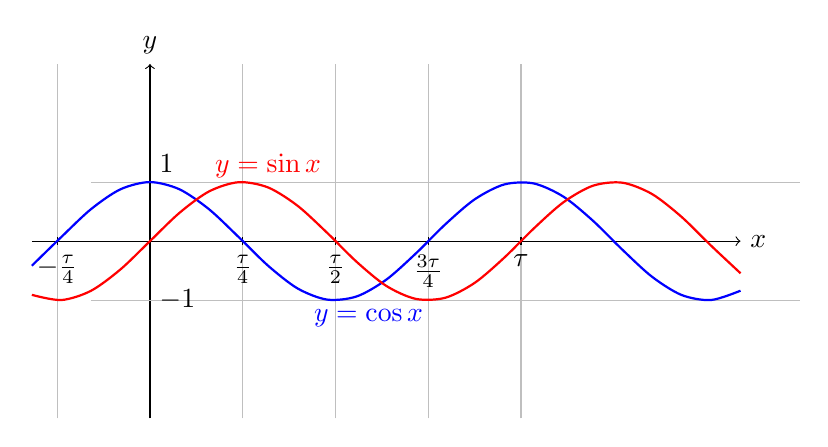
\begin{tikzpicture}[scale=0.75]
  \draw[->] (-2,0) -- (10,0) node[right] {$x$};
  \draw[->] (0,-3) -- (0,3) node[above] {$y$};
  \foreach \x/\xtext in
    {{pi/2}/{\frac \tau 4}, {pi}/{\frac \tau 2},
     {2*pi}/{\tau}, {3*pi/2}/{\frac {3\tau} 4}, {-pi/2}/{-\frac {\tau}{4}}} {
    \draw[shift={(\x,0)},lightgray] (0,-3) -- (0,3);
    \draw[shift={(\x,0)}] (0pt,2pt) -- (0pt,-2pt) node[below] {$\xtext$};
  }
  \foreach \y in {1, -1} {
    \draw[shift={(0,\y)},lightgray] (-1,0) -- (11,0);
  }
  \draw (0,1) node [above right] {$1$};
  \draw (0,-1) node [right] {$-1$};
  \draw[domain=-2:10,smooth,variable=\x,blue,thick] plot ({\x},{cos(deg(\x))});
  \draw[domain=-2:10,smooth,variable=\x,red,thick] plot ({\x},{sin(deg(\x))});
  \draw (3.7,-1) node[blue,below] {$y=\cos x$};
  \draw (2,0.9)  node[red,above] {$y=\sin x$};
  \end{tikzpicture}
  \caption{%
  I grafici delle funzioni $\sin$, $\cos$ di 
  un generico periodo $\tau$.}
\end{figure}

\section{costruzione degli insiemi numerici}
\label{sec:costruzione}

\subsection{costruzione dell'insieme dei numeri naturali}

\begin{theorem}[esistenza dei numeri naturali]
  \label{th:esistenza_naturali}%
Se $X$ è un qualunque insieme infinito (definizione~\ref{def:infinito})
esistono $\NN\subset X$, $0\in \NN$ e $\sigma\colon \NN\to\NN$ 
che soddisfano gli assiomi di Peano (teorema~\ref{def:naturali}).
\end{theorem}
%
\begin{proof}
Se $X$ è infinito esiste $f\colon X\to X$ iniettiva ma non suriettiva. 
Scegliamo arbitrariamente $0\in X\setminus f(X)$. 
Preso un sottoinsieme $I\subset X$ diremo che $I$ è \emph{induttivo}
\mymargin{induttivo}%
\index{induttivo}%
se $0\in I$ e $n\in I\implies f(n)\in I$. 
Possiamo quindi definire:
\[
  \NN = \bigcap \ENCLOSE{I\subset X\colon \text{$I$ induttivo}}.
\]
Si verifica facilmente che $\NN$ è anch'esso un sottoinsieme induttivo di $X$.
\mynote{Nella definizione~\ref{def:restrizione} viene introdotto il simbolo
$\llcorner$ per la restrizione di funzione.}
Dunque per ogni $n\in \NN$ si ha $f(n)\in \NN$ e quindi possiamo 
definire $\sigma\colon \NN\to \NN$ come la restrizione di $f$ 
ad $\NN$: $\sigma=f\llcorner \NN$.

Osserviamo quindi che $\sigma$ soddisfa gli assiomi di Peano.
Il primo assioma è conseguenza dell'iniettività di $f$.
Il secondo è verificato per come abbiamo scelto $0$.
Per verificare il terzo assioma consideriamo un qualunque insieme 
$A\subset \NN$ tale che $0\in A$ e tale che se $n\in A$ anche $n+1\in A$.
Per definizione $A$ è induttivo e quindi certamente 
$\NN\subset A$ visto che $\NN$, per come è definito,
è sottoinsieme di ogni insieme induttivo.
\end{proof}

La costruzione precedente ci dice che l'insieme $\NN$ è il più piccolo insieme infinito
nel senso che: se $X$ è infinito allora $\# X \ge \# \NN$. 
\mynote{Questa osservazione ci dice che se $\NN$ e $\NN'$ sono due diversi insiemi di 
numeri naturali allora $\#\NN\le \#\NN'$ e $\#\NN'\le\#\NN$ per cui, 
grazie al teorema~\ref{th:cantor_bernstein}, $\# \NN = \# \NN'$.
Nel teorema~\ref{th:unicitaN} vedremo che non solo esiste una corrispondenza biunivoca 
tra $\NN$ e $\NN'$ ma anche che esiste 
una corrispondenza che preserva la struttura 
(l'operazione $\sigma$ e l'elemento $0$). 
}


%% \begin{comment} % DOVE SI USA?
%%   \begin{lemma}
%%     Per ogni $n\in \NN$ si ha $\sigma(n)\neq n$.
%%     \end{lemma}
%%     \begin{proof}
%%       Lo si dimostra per induzione. Per $n=0$ sappiamo che $\sigma(0)\neq 0$ 
%%       in quanto zero non è successore di nessun numero naturale.
%%       Se ora supponiamo di sapere che $\sigma(n)\neq n$ sapendo che 
%%       $\sigma$ è iniettiva possiamo dedurre $\sigma(\sigma(n))\neq \sigma(n)$ 
%%       che è proprio il passo induttivo.
%%   \end{proof}    
%% \end{comment}

\begin{theorem}[definizione per induzione]
  \label{th:induzione}%
  Sia $X$ un insieme, sia $\alpha\in X$ e sia $g\colon X\to X$ una funzione.
  Allora esiste una unica funzione $f\colon \NN \to X$ tale che
  \begin{equation}\label{eq:4835628}
    \begin{cases}
      f(0) = \alpha, \\
      f(\sigma(n)) = g(f(n)).
    \end{cases}
  \end{equation}
  Si avrà dunque
  \[
    f(0) = \alpha,\quad
    f(1) = g(\alpha),\quad
    f(2) = g(g(\alpha)),\quad
    f(3) = g(g(g(\alpha)))\dots
  \]
  Più in generale se abbiamo $\alpha\in X$ e una funzione $g\colon \NN \times X \to X$
  esisterà una unica funzione $f\colon \NN \to X$ tale che
  %
  \begin{equation}
    \begin{cases}
      f(0) = \alpha, \\
      f(\sigma(n)) = g(n, f(n)).
    \end{cases}
  \end{equation}
\end{theorem}
%
\begin{proof}
Dobbiamo ricordarci che le funzioni $f\colon \NN \to X$ non sono altro che relazioni 
e cioè sottoinsiemi del prodotto $\NN\times X$.
L'idea è quindi di prendere il più piccolo sottoinsieme di $\NN\times X$ 
che possa rappresentare una funzione con le proprietà richieste.
Consideriamo dunque la famiglia di insiemi:
\[
\mathcal F = \ENCLOSE{F\in \mathcal P(\NN\times X)\colon 
  (0,\alpha)\in F,\quad (n,x)\in F \Rightarrow (\sigma(n),g(x))\in F}.
\]
Chiaramente $\mathcal F$ non è vuota in quanto $\NN\times X \in \mathcal F$.
Possiamo dunque farne l'intersezione e definire un insieme $f$:
\[
  f = \bigcap_{F\in \mathcal F} F.
\]
L'insieme $f$ che abbiamo definito rappresenta una relazione tra $\NN$ e $X$.
Visto che $(0,\alpha)\in F$ per ogni $F\in \mathcal F$ dovrà essere 
$(0,\alpha)\in f$.
Inoltre se $(n,x)\in f$ allora $(n,x)\in F$ per ogni $F\in \mathcal F$ 
e quindi $(\sigma(n),g(x))\in F$ per ogni $F\in \mathcal F$
da cui $(\sigma(n),g(x))\in f$. Significa che $f\in \mathcal F$.

Vogliamo ora dimostrare che $f$ è una funzione, cioè che è univocamente definita 
su tutto $\NN$.
Per prima cosa consideriamo l'insieme su cui $f$ è definita 
e cioè $A=\ENCLOSE{n\in \NN\colon \exists x\in X\colon (n,x)\in f}$
e dimostriamo, per induzione, che $A=\NN$.
In effetti $(0,\alpha)\in f$ quindi $0\in A$. 
E se $n\in A$ sappiamo che esiste $x\in X$ tale che $(n,x)\in f$ 
e dunque, essendo $f\in \mathcal F$, anche $(\sigma(n),g(x))\in f$
da cui $\sigma(n)\in A$. 
Abbiamo dimostrato che $f$ è definita su tutto $\NN$.

Dimostriamo ora che $f$ è univoca. Consideriamo 
l'insieme su cui $f$ è univocamente definita: 
$B=\ENCLOSE{n\in \NN\colon \exists! x\in X\colon (n,x)\in f}$.
Di nuovo vogliamo dimostrare per induzione che $B=\NN$. 
Per dimostrare che $0\in B$, visto che già sappiamo che $(0,\alpha)\in f$, 
dobbiamo dimostrare che se $x\neq \alpha$ si ha $(0,x)\not\in f$.
Sia dunque $x\neq \alpha$ e consideriamo 
l'insieme $F=f\setminus\ENCLOSE{(0,x)}$.
Chiaramente $F\in \mathcal F$ in quanto $(0,\alpha)\in F$
visto che $(0,\alpha)\in f$ e $(0,\alpha)\neq (0,x)$
inoltre se $(n,y)\in F$ allora $(n,y)\in f$ 
e quindi $(\sigma(n),g(y)) \in f$.
Ma certamente $(\sigma(n),g(y))\neq (0,x)$ in quanto $\sigma(n)\neq 0$ 
dunque $(\sigma(n),g(y))\in F$.
Visto che $F\in \mathcal F$ si deve avere $f\subset F$ e dunque 
$(0,x)\not \in f$. Dunque $f$ è univocamente definita in $0$.

Dobbiamo ora mostrare che se $n\in B$ anche $\sigma(n)\in B$.
Se $n\in B$ significa che c'è un unico $x\in X$ tale che $(n,x)\in f$
e certamente anche $(\sigma(n),g(x))\in f$.
Prendiamo allora $y\neq g(x)$, vorremo dimostrare che $(\sigma(n),y)\not \in f$.
Consideriamo, similmente a prima, l'insieme $F=f\setminus\ENCLOSE{(\sigma(n),y)}$
e cerchiamo di dimostrare che $F\in \mathcal F$.
Chiaramente $(0,\alpha)\in F$ perché $(0,\alpha)\in f$ 
e non può essere $(0,\alpha)=(\sigma(n),y)$ in quanto $\sigma(n)\neq 0$.
Se ora supponiamo che sia $(m,z)\in F$ certamente sarà $(m,z)\in f$ 
e dunque $(\sigma(m),g(z))\in f$: 
dobbiamo mostrare che $(\sigma(m),g(z))\in F$. 
D'altra parte se fosse $(\sigma(m), g(z))=(\sigma(n),y)$ 
dovrebbe essere $m=n$ in quanto $\sigma$ è iniettiva. 
Ma visto che $f$ è univocamente definita su $n$ dovrà allora essere 
anche $(n,z) = (n,x)$ e quindi $g(z)=g(x) \neq y$. 
Dunque $(\sigma(m),g(z))\in F$ e $F\in \mathcal F$.
Ma allora $f\subset F$ e quindi $(\sigma(n),y)\not \in f$.
Significa che $f$ è univocamente definita anche in $\sigma(n)$.
Per induzione $B=\NN$ ed $f$ è una funzione $f\colon \NN\to X$.

Ovviamente visto che $f\in \mathcal F$ sappiamo che $f$ 
soddisfa le proprietà richieste dal teorema.

Nella seconda parte del teorema, dove $g\colon \NN\times X \to X$,
possiamo considerare l'insieme $Y=\NN\times X$ e la funzione 
$G\colon Y\to Y$ definita da $G(n,x) = (\sigma(n), g(n,x))$.
Allora applicando la prima parte possiamo trovare $F\colon \NN\to Y$
tale che $F(0) = (0,\alpha)$ e $F(\sigma(n)) = G(F(n))$.
Basterà prendere come $f(n)$ la seconda componente di $G(n)$.
\end{proof}
  
In particolare il teorema precedente ci permette di definire l'iterata $n$-esima $f^n$ 
di una qualunque funzione $f\colon X\to X$.
Se $\id_X\colon X\to X$ rappresenta la funzione identità su $X$:
$\id_X(x)=x$,
possiamo definire:
\index{iterazioni}%
\index{funzione!iterata}%
\index{funzione!composta}%
\begin{equation}\label{def:iterata}
  \begin{cases}
    f^0 = id_X,\\
    f^{\sigma(n)} = f\circ f^n.
  \end{cases}
\end{equation}

Le iterate della funzione $\sigma$ ci permettono di definire l'addizione:
\begin{equation}\label{def:addizione}
  n+k = \sigma^k(n).  
\end{equation}
Definita in questo modo l'addizione $+$ è una funzione 
che ad ogni $k\in \NN$ associa la funzione $\sigma^k$
che a sua volta ad ogni $n\in \NN$ associa $\sigma^k(n)=n+k$.
Si ha dunque $+\colon \NN \to (\NN\to \NN)$.
Si potrebbe anche pensare all'addizione come ad una funzione 
che ad ogni coppia $(n,k)\in \NN\times \NN$ associa 
la somma $n+k\in \NN$. Dunque si avrebbe $+\colon (\NN\times \NN)\to \NN$.
Ovviamente le due definizioni sono equivalenti, 
il grafico della prima funzione è composto dai punti 
$(k,(n,n+k))\in \NN\times (\NN\times \NN)$
mentre nel secondo caso i punti sono $((n,k),n+k)\in (\NN\times \NN)\times \NN$.
Il vantaggio di definire una funzione $\NN\to(\NN\to\NN)$ invece che una 
funzione $(\NN\times\NN)\to\NN$ è che nel primo caso possiamo utilizzare 
una definizione per induzione. 
In effetti la definizione~\eqref{def:addizione} è equivalente 
a definire l'addizione come l'unica operazione su $\NN$ tale che:
\[
\begin{cases}
  n+0=n\\
  n+(k+1)=(n+k)+1.
\end{cases}  
\]

% \begin{theorem}
%   \label{th:iterata_composta}%
%   Sia $f\colon A \to A$ una qualunque funzione.
%   Allora 
%   \begin{equation}\label{eq:iterata_composta}
%     f^{n+m} = f^m \circ f^n = f^n \circ f^m.
%   \end{equation}
% \end{theorem}
% %
% \begin{proof}
% Dimostriamo la prima uguaglianza in~\eqref{eq:iterata_composta} 
% per induzione su $m$.
% Per $m=0$ è ovvio in quanto $n+0 = \sigma^0(n)=\id_{\NN}(n)=n$ e $f^m=\id_A$
% dunque $f^{n+0} = f^n = f^0 \circ f^n$.
% Il passo induttivo richiede \eqref{eq:476554},
% \eqref{def:iterata} e l'ipotesi induttiva~\eqref{eq:iterata_composta}:
% \[
% f^{n+\sigma(m)} 
% = f^{\sigma(n+m)}
% = f\circ f^{n+m}
% = f\circ f^m \circ f^n
% = f^{\sigma(m)}\circ f^n.
% \]
% 
% Per dimostrare la seconda uguaglianza in~\eqref{eq:iterata_composta}
% dobbiamo preliminarmente dimostrare che vale 
% \begin{equation}\label{eq:5ty349}
%   f\circ f^n = f^n \circ f.  
% \end{equation}
% Lo facciamo per induzione su $n$. Se $n=0$ ambo i lati sono uguali a $f$.
% Il passaggio induttivo è il seguente:
% \[
%   f\circ f^{\sigma(n)} = f\circ f\circ f^n = f\circ f^n \circ f 
%   = f^{\sigma(n)} \circ f.
% \]
% Allora possiamo dimostrare, per induzione su $m$, 
% che $f^m\circ f^n = f^n\circ f^m$:
% \[
%   f^{\sigma(m)}\circ f^n 
%   = f\circ f^m \circ f^n 
%   = f\circ f^n \circ f^m
%   = f^n \circ f\circ f^m
%   = f^n \circ f^{\sigma(m)}.
% \]
% \end{proof}

\begin{theorem}\label{th:proprieta_addizione}
  L'addizione su $\NN$ soddisfa le seguenti 
  proprietà:
  \begin{enumerate}
    \item associativa: $(n+m)+k = n + (m + k)$,
    \item elemento neutro: $n+0 = n = 0+n$,
    \item commutativa: $n+m = m+n$,
    \item invariantiva: se $m+k = n+k$ allora $m=n$.
  \end{enumerate}
\end{theorem}
\begin{proof}
Le proprietà andranno dimostrate per induzione.
I casi base sono sempre banali, vediamo i passi induttivi.

Per la proprietà associativa si ha
\[
(n+m)+(k+1) 
= ((n+m)+k)+1 
= (n+(m+k))+1
= n +((m+k)+1)
= n + (m + (k+1)).
\]
Per l'elemento neutro $n+0=n$ per definizione. Mentre:
\[
0+(n+1) = (0+n)+1 = n+1.
\]
Per la proprietà commutativa dobbiamo prima dimostrare che $n+1=1+n$.
Ma infatti per induzione si ha $n+1+1 = 1+n+1$.
Allora il passo induttivo della proprietà commutativa risulta:
\[
n + m + 1 
= m + n + 1
= m + 1 + n.
\]

Per dimostrare la proprietà invariantiva se vale $m+k+1=n+k+1$
allora $\sigma(m+k)=\sigma(n+k)$ ed essendo $\sigma$ iniettiva 
possiamo dedurre $m+k=n+k$. Ma allora, per ipotesi induttiva, $m=n$. 
\end{proof}

% \begin{exercise}
%   Dimostrare, utilizzando il principio di induzione e le proprietà 
%   dell'addizione, la seguente 
%   proposizione:
%   \[
%   \forall n\in \NN\colon \enclose{\enclose{\exists m\in \NN \colon n = m + m} 
%   \lor \enclose{\exists m\in \NN\colon n = m + m + 1}}.  
%   \]
% \end{exercise}

% La moltiplicazione $\cdot$ su $\NN$ è intesa come somma ripetuta:
% $3\cdot n = n + n + n$. 

% Possiamo ora definire la moltiplicazione su $\NN$ come addizione ripetuta.
% Formalmente è l'unica operazione che soddisfa la seguente definizione 
% induttiva:
% \[
% \begin{cases}
%   n\cdot 0 = 0,\\
%   n\cdot(k+1) = n\cdot k + k.
% \end{cases}  
% \]

% Chiaramente $(\sigma^n)^0=\id_\NN$ dunque $n\cdot 0=\id(0) = 0$.
% Mentre $(\sigma^n)^1=\sigma^n$ dunque $n\cdot 1 = \sigma^n(0) = n$.  
% 
% Ci servirà anche osservare che risulta:
% \begin{equation}\label{eq:70138875}
%   n\cdot (k+1) = n\cdot k + n
% \end{equation}
% infatti:
% \[
%  n\cdot(k+1) 
%  = (\sigma^n)^{k+1}(0)  
%  = \sigma^n ((\sigma^n)^k(0))
%  = \sigma^n (n\cdot k) = n\cdot k + n.
% \]
% 
% La moltiplicazione tra naturali è legata 
% alle iterazioni dai seguenti teoremi.
% \begin{theorem}
%   \label{th:commuta_composta}%
%   Se $f,g\colon X\to X$ commutano, cioè se $f\circ g = g\circ f$ 
%   allora per ogni $n\in \NN$ anche $f^n$ e $g$ commutano
%   e inoltre si ha:
%   \begin{equation}\label{eq:commuta_composta}
%     f^n\circ g^n = (f\circ g)^n.
%   \end{equation}
% \end{theorem}
% \begin{proof}
% Supponiamo ora che $f\circ g = g\circ f$ e dimostriamo per 
% induzione che $f^n\circ g = g\circ f^n$:
% \[
% f^{n+1}\circ g 
% = f \circ f^n \circ g 
% = f \circ g \circ f^n 
% = g \circ f \circ f^n
% = g \circ f^{n+1}.
% \]
% Possiamo quindi dimostrare per induzione che $f^n\circ g^n = (f\circ g)^n$:
% \[
% f^{n+1}\circ g^{n+1}
% =f\circ f^n \circ g \circ g^n
% =f\circ g\circ f^n\circ g^n 
% = (f\circ g) \circ (f\circ g)^n
% = (f\circ g)^{n+1}. 
% \]
% \end{proof}
% 
% \begin{theorem}[iterata dell'iterata]
% Sia $f\colon X\to X$ una funzione qualunque e siano $n,m\in\NN$.
% Allora 
% \begin{equation}\label{eq:iterazione_iterazione}
%   f^{n\cdot m} = (f^n)^m = (f^m)^n.    
% \end{equation}
% \end{theorem}
% %
% \begin{proof}
% Dimostriamo entrambe le uguaglianze per induzione su $m$.
% Per $m=0$ tutti e tre i termini sono uguali all'identità.
% 
% Il passo induttivo per dimostrare $f^{n\cdot m}=(f^n)^m$ 
% usa~\eqref{eq:70138875}:
% \[
% f^{n\cdot (m+1)}
% =f^{n\cdot m + n } 
% = f^n \circ f^{n\cdot m}
% = f^n \circ (f^n)^m
% = (f^n)^{m+1}.
% \]
% 
% Per dimostrare $(f^n)^m = (f^m)^n$ 
% il passo induttivo sfrutta~\eqref{eq:iterazione_iterazione}
% e~\eqref{eq:commuta_composta}:
% \[
% (f^n)^{m+1}
% = f^n \circ (f^n)^m
% = f^n \circ (f^m)^n
% = (f\circ f^m)^n
% = (f^{m+1})^n.
% \]
% \end{proof}
% 
\begin{theorem}[proprietà della moltiplicazione]
  \label{th:proprieta_moltiplicazione}%
La moltiplicazione su $\NN$ soddisfa le seguenti proprietà:
\begin{enumerate}
  \item elemento neutro e assorbente: $n\cdot 1=n$, $n\cdot 0=0$,
  \item proprietà commutativa: $n\cdot m = m\cdot n$.
  \item proprietà distributiva: $n\cdot(k+j) = n\cdot k + n\cdot j$,
  \item proprietà associativa: $n\cdot(m\cdot k) = (n\cdot m)\cdot k$,
\end{enumerate}
\end{theorem}
\begin{proof}
  L'elemento assorbente è dato per definizione: $n\cdot 0 = 0$.
  Per l'elemento neutro si ha $n\cdot 1 = n\cdot 0 + n = 0+n=n$.

  Le altre proprietà andranno tutte dimostrate 
  per induzione. 
  I casi base saranno sempre banali, ci limitiamo a verificare 
  i passi induttivi. 

  Per la proprietà commutativa verifichiamo innanzitutto che 
  $(m+1)\cdot n = m\cdot n + n$. 
  Il passo induttivo è
  \[
  (m+1)\cdot(n+1) 
  = (m+1)\cdot n + m + 1  
  = m\cdot n + n + m + 1
  = m\cdot (n+1) + n + 1. 
  \]
  Allora il passo induttivo della proprietà commutativa risulta:
  \[
  n\cdot (m+1) 
  = n\cdot m + n 
  = m \cdot n + n 
  = (m+1)\cdot n.  
  \]
  Per la proprietà distributiva:
  \begin{align*}
  (n+1)\cdot(k+j) 
  &= (k+j)\cdot (n+1)  
  = (k+j)\cdot n + k + j
  = n\cdot(k+j) + k + j\\
  &= n\cdot k +k + n\cdot j + j
  = (n+1)\cdot k + (n+1)\cdot j.
  \end{align*}
  Infine la proprietà associativa:
  \[
  n\cdot(m\cdot(k+1))
  = n\cdot (m\cdot k + m) 
  = n\cdot (m\cdot k) + n\cdot m
  = (n\cdot m)\cdot k + n\cdot m
  = (n\cdot m)\cdot (k+1). 
  \]
\end{proof}

% L'elevamento a potenza si definisce come un prodotto ripetuto: 
% $k^3 = k\cdot k\cdot k$.
% Se consideriamo la funzione $\cdot k$ 
% che moltiplica un numero naturale per $k$:
% \[
%  \cdot k(n) = n\cdot k  
% \]
% Possiamo definire le potenze di $k$ in questo modo:
% \[
%    k^n = (\cdot k)^n(1).  
% \]
% Osserviamo che più in generale si ha 
% \begin{equation}\label{eq:3954820}
%   (\cdot k)^n(m) = m\cdot k^n
%   \qquad\text{ovvero}\qquad
%  (\cdot k)^n = \cdot(k^n).
% \end{equation}
% 

% Definiamo l'operazione \emph{potenza} $m^n$ su $\NN$ come un prodotto 
% ripetuto, mediante la seguente definizione per induzione:
% \[
% \begin{cases}
%   m^0 = 1\\
%   m^{n+1} = m\cdot m^n.
% \end{cases}  
% \]
\begin{theorem}[proprietà delle potenze]
  \label{th:proprieta_potenza}%
  L'elevamento a potenza definito su $\NN$ ha le seguenti proprietà
  (per ogni $k,n,m\in \NN$):
  \begin{enumerate}
    \item $k^0 = 1$,
    \item $k^{n+m} = k^n \cdot k^m$,
    \item $(k^n)^m = k^{n\cdot m}$,
    \item $(k\cdot j)^n = k^n\cdot j^n$. 
  \end{enumerate}
\end{theorem}
%
\begin{proof}
La prima proprietà $k^0=1$ è data per definizione.

Le altre proprietà si dimostrano per induzione.
I casi base sono tutti banali, ci limitiamo quindi 
a mostrare i passi induttivi.

Per dimostrare $k^{n+m}=k^n\cdot k^m$ il passo induttivo è:
\[
k^{n+m+1} 
= k\cdot k^{n+m}  
= k\cdot k^n\cdot k^m
= k^n \cdot k^{m+1}.
\]

Per dimostrare $(k^n)^m = k^{n\cdot m}$ il passo induttivo è 
\[
  (k^n)^{m+1} 
  = k^n\cdot (k^n)^m
  = k^n\cdot k^{n\cdot m}
  = k^{n+n\cdot m}
  = k^{n\cdot(m+1)}.
\]

Infine per dimostrare $(k\cdot j)^n = k^n\cdot j^n$ 
il passo induttivo è
\[
(k\cdot j)^{n+1} 
= k\cdot j\cdot (k\cdot j)^n  
= k\cdot j\cdot k^n\cdot j^n
= k^{n+1}\cdot j^{n+1}.
\]
\end{proof}

Possiamo definire la relazione $\le$ su $\NN$ ponendo 
\[
  m \le n \iff \exists k\in \NN\colon n = m+k.  
\]
Se $m\le n$ tale numero 
$k$ è unico in quanto se fosse $m+j=n=m+k$ potremmo dedurre $k=j$
dalla proprietà invariantiva della addizione. 
Possiamo dunque definire la \emph{differenza}%
\mymargin{differenza}%
\index{differenza}: $k=n-m$.

\begin{theorem}
  \label{th:proprieta_ordine_N}
La relazione $\le$ è una relazione d'ordine totale su $\NN$.
\end{theorem}
%
\begin{proof}
  Il fatto che $x+0=x$ dimostra la proprietà riflessiva.
  
  Per la proprietà transitiva è sufficiente osservare
  che se $y=x+k$ e $z=y+j$ allora $z=x+k+j$.

  Per la proprietà antisimmetrica supponiamo di avere $x=y+k$ 
  e $y=x+j$. Deduciamo che $x+k+j = y +k+j$ da cui $x=y$
  per la proprietà invariantiva dell'addizione.
  
  Per mostrare che l'ordinamento è totale dobbiamo invece 
  procedere con una dimostrazione per induzione. 
  Per induzione su $x\in \NN$ vogliamo mostrare 
  che per ogni $y\in \NN$ si ha $x\le y$ oppure $y\le x$. 
  Se $x=0$ il fatto è ovvio in quanto $y=y+0$ e quindi $y\ge 0$
  per ogni $y\in \NN$.
  Supponiamo ora di sapere che $x\le y$ oppure $y\le x$.
  Se $y\le x$ significa che $x = y + k$ per un qualche 
  $k\in \NN$. Ma allora $x+1 = y + k + 1$ e quindi 
  vale anche $y\le x+1$. 
  Se invece $x\le y$ significa che esiste $k\in \NN$ 
  per cui $y=x+k$. Se $k\neq 0$ allora $k=1+j$ con $j\in \NN$
  da cui $y=x+1+j$ e dunque anche $x+1\le y$.
  Se $k=0$ allora $x=y$ e dunque $x+1=y+1$ che ci porta 
  alla disuguaglianza inversa $x+1\ge y$.
  In ogni caso il passo induttivo è dimostrato.
\end{proof}

\begin{theorem}[proprietà di monotonia sui naturali]
  \label{th:monotonia_naturali}%
  Se $m,n,k\in \NN$ e $m\le n$ allora si ha 
  \[
    m+k\le n+k,
    \qquad 
    m\cdot k \le n\cdot k,
    \qquad
    m^k\le n^k,
    \qquad
    k^m\le k^n.
  \]
\end{theorem}
\begin{proof}
  Se $m\le n$ si ha $n=m+j$. 
  Dunque
  \[
  n+k = m + j + k \ge m+k   
  \] 
  e
  \[
  m\cdot k = (n+j)\cdot k = n\cdot k + j\cdot k \ge n\cdot k.  
  \]

  Per la monotonia delle potenze procediamo per induzione.
  Basterà dimostrare che $m^k\le(m+1)^k$ e $k^m\le k^{m+1}$.
  Lo facciamo, a loro volta, per induzione:
  \[
  (m+1)^{k+1} = (m+1)\cdot (m+1)^k \ge m\cdot m^k
  \]
  e (supponendo $k\ge 1$)
  \[
  k^{m+1} = k\cdot k^m \ge 1\cdot k^m = k^m. 
  \]
\end{proof}

\subsection{buon ordinamento e unicità dei numeri naturali}

\begin{theorem}[principio del buon ordinamento]
  \label{th:buon_ordinamento}
  Sia $A\subset \NN$, $A\neq \emptyset$. 
  Allora $A$ ha minimo.
\end{theorem}
%
\begin{proof}
  Osserviamo che se $n\in \NN$ è un minorante di $A\subset \NN$ 
  allora o $n\in A$ e quindi $n$ è il minimo di $A$
  oppure anche $n+1$ è un minorante di $A$ in quanto 
  non ci sono numeri naturali strettamente compresi tra $n$ e $n+1$.
  \mynote{Se ci fosse un numero naturale tra $n$ e $n+1$ 
  sottraendo $n$ avremmo un numero naturale tra $0$ e $1$. 
  Ma non esiste $x\in \NN$ tale che $0<x<1$.
  Infatti se $x\in \NN$, $x>0$ allora $x\neq 0$ e quindi 
  esiste $m\in \NN$ tale che $x=m+1$. 
  Ma allora $x\ge 1$.}
  Dunque se $A$ non avesse minimo, per il principio di induzione 
  ogni $n\in\NN$ sarebbe un minorante di $A$.
  In tal caso $A$ dovrebbe essere vuoto perché se esistesse $a\in A$ 
  certamente $a+1$ non sarebbe un minorante di $A$.
\end{proof}

Vogliamo ora dimostrare che l'insieme dei numeri naturali è sostanzialmente 
unico nel senso che se ci sono due insiemi che soddisfano gli assiomi di 
Peano allora è possibile mettere in corrispondenza gli elementi dei due insiemi 
in modo che lo zero vada in zero e numeri corrispondenti abbiano successori 
corrispondenti.

\begin{theorem}[unicità dei numeri naturali]
  \label{th:unicitaN}%
  Se $\NN$ e $\NN'$ sono due insiemi che soddisfano gli assiomi di Peano 
  con zero $0\in \NN$ e $0'\in \NN'$ e funzioni 
  successore $\sigma$ su $\NN$ e $\sigma'$ su $\NN'$ allora
  esiste una funzione bigettiva $f\colon \NN\to \NN'$ tale che 
  $f(0) = 0'$ e $f(\sigma(n)) = \sigma'(f(n))$.
\end{theorem}
%
\begin{proof}
Possiamo definire $f$ per induzione:
\[
\begin{cases}
  f(0) = 0' \\ 
  f(\sigma(n)) = \sigma'(f(n))
\end{cases}  
\]
così rimane solo da dimostrare che $f$ è una bigezione.

Per dimostrare che $f$ è iniettiva consideriamo l'insieme 
\[
  A=\ENCLOSE{a\in \NN\colon \exists b\in \NN\colon b\neq a, f(a)=f(b)}.
\]
Se tale insieme è vuoto allora $f$ è effettivamente iniettiva.
Supponiamo allora per assurdo che $A$ non sia vuoto.
In tal caso possiamo considerare il minimo $a=\min A$ 
(grazie al teorema~\ref{th:buon_ordinamento}).
Dovrà quindi esistere $b\in \NN$ tale che $b\neq a$ e $f(b)=f(a)$.
Ovviamente anche $b\in A$ e quindi dovrà essere $b>a$ in quanto
$a$ è il minimo. Dunque $b>0$ e $f(b) = f(\sigma(b-1))
=\sigma'(f(b-1))$. Se $a=0$ abbiamo $f(a)=0'$ e quindi da $f(a)=f(b)$ 
otteniamo che $0'$ è nell'immagine di $\sigma'$ che è contrario 
agli assiomi di Peano. 
Se invece $a>0$ si avrà, come per $b$,
$f(a)=\sigma'(f(a-1))$ e dunque $\sigma'(f(a-1)) = \sigma'(f(b-1))$.
Per l'iniettività di $\sigma'$ si deduce $f(a-1)=f(b-1)$ da cui 
$a-1 \in A$. Ma questo è assurdo in quanto $a$ era il minimo di $A$.

Per dimostrare che $f$ è surgettiva consideriamo l'immagine 
$B'=f(\NN)$ e usiamo il principio di induzione su $\NN'$ 
per dimostrare che $B'=\NN'$.
Per prima cosa $0'\in B'$ in quanto $0'=f(0)$.
Se poi $n'\in B'$ allora esiste $n\in \NN$ tale che $f(n)=n'$.
Ma allora $f(\sigma(n))=\sigma'(f(n))=\sigma'(n')$ 
e dunque anche $\sigma'(n')\in B$. 
\end{proof}

\subsection{costruzione dell'insieme dei numeri interi}

L'insieme $\NN$ dei numeri naturali con l'operazione di addizione 
non è un gruppo in quanto gli elementi non hanno opposto in $\NN$.
Per ovviare a questo dobbiamo definire un insieme più grande che 
contenga la differenza $n-m$ di ogni coppia $(m,n)$ di numeri naturali.
\mynote{Osserviamo che la coppia $(m,n)$ può anche essere denotata 
con $m\mapsto n$ e l'insieme delle coppie $m\mapsto n$ con
differenza costante $n-m$, non è altro che il grafico della 
traslazione $\NN\to \NN$ che manda $m$ in $n$. 
Stiamo quindi dicendo che i numeri interi sono le traslazioni 
(in avanti o indietro) dei numeri naturali.}
Ovviamente coppie diverse possono avere la stessa differenza quindi 
dobbiamo definire una relazione di equivalenza che identifichi le coppie 
che rappresentano lo stesso numero. 

Possiamo dunque definire 
\[
  \ZZ \defeq (\NN \times \NN)/\sim
  \qquad\text{dove}\qquad
  (m,n)\sim (m',n')\iff n+m' = n'+m.
\]
Un numero intero $k\in \ZZ$ sarà quindi una classe di equivalenza:
$k = \Enclose{(m,n)}$ (intuitivamente il numero intero $\Enclose{(m,n)}$ 
con $n,m\in \NN$ 
rappresenta il numero $n-m\in \ZZ$).
L'addizione su $\ZZ$ si definisce facilmente:
\[
 \Enclose{(m,n)}+\Enclose{(M,N)} = \Enclose{(m+M,n+N)}.
\]
\mynote{Se i numeri interi vengono interpretati come \emph{traslazioni}
dei numeri naturali la somma di due numeri interi non è altro che 
la composizione delle due traslazioni.}
Si verifica facilmente che la definizione precedente è \emph{ben posta}
ovvero non dipende dalla scelta di $(n,m)$ e $(N,M)$ all'interno 
della loro classe di equivalenza: se $n+m' = n'+m$ e $N+M'=N'+M$ 
allora $(n+N)+(m'+M')=(n'+N')+(m+M)$.

L'addizione che abbiamo definito su $\ZZ$ è commutativa e associativa, 
il numero $\Enclose{(0,0)}$
è elemento neutro e ogni elemento ha opposto, infatti 
$\Enclose{(m,n)} + \Enclose{(n,m)} = \Enclose{(m+n,n+m)}=\Enclose{(0,0)}$
cioè $-\Enclose{(m,n)}=\Enclose{(n,m)}$.
Dunque $\ZZ$ è un gruppo additivo.

Possiamo facilmente definire un ordinamento su $\ZZ$:
$\Enclose{(m,n)} \ge \Enclose{(M,N)}$ se 
$n+M\ge N+m$.
E' molto facile verificare che l'ordinamento è compatibile 
con l'addizione e quindi $\ZZ$ risulta essere un gruppo abeliano ordinato.

Osserviamo che possiamo identificare un numero naturale $n\in \NN$ 
con la classe di equivalenza $\phi(n) = \Enclose{(0,n)}\in \ZZ$.
La corrispondenza $\phi\colon \NN\to\ZZ$ rispetta sia l'addizione,
$\phi(n+m) = \phi(n)+\phi(m)$ che l'ordinamento $n\ge m \iff \phi(n)\ge \phi(m)$.
Dunque l'insieme $\phi(\NN)\subset \ZZ$ è una copia isomorfa dei 
numeri naturali. 
\mynote{
Se $n,m\in \NN$, $n\ge m$ risulta 
$\Enclose{(m,n)} = \Enclose{(n,0)}-\Enclose{(m,0)} = \phi(n)-\phi(m)$.
}%
Sarà quindi comodo rinominare $\NN$ identificandolo con $\phi(\NN)$ così 
ottenendo che $\NN\subset \ZZ$.
Preso qualunque $n\in \ZZ$ si avrà che $n\in \NN$ se $n\ge 0$ altrimenti 
si avrà $-n\in \NN$. 
Dunque $\ZZ = \NN \cup (-\NN)$ e $0\in \NN\subset \ZZ$ 
è l'unico numero intero che è l'opposto di se stesso.

L'operazione di moltiplicazione che abbiamo definito su $\NN$ può essere 
estesa in modo naturale a tutto $\ZZ$. 
Se vogliamo mantenere la proprietà distributiva dovremo avere, 
per $n,m\in\NN$
\[
  0 = 0 \cdot n = (m+(-m))\cdot n = m\cdot n + (-m)\cdot n
\]
per cui poniamo, per definizione, per ogni $n,m\in \NN$:
\[
  (-m) \cdot n = -(m\cdot n), \qquad  m \cdot (-n) = -(m\cdot n).
\]
In questo modo la moltiplicazione $x\cdot y$ 
è ben definita per ogni $x,y\in \ZZ$ e soddisfa la proprietà distributiva.

Con le definizioni date è noioso ma facile dimostrare 
che valgono le usuali proprietà della
moltiplicazione su $\ZZ$.

\begin{theorem}[proprietà moltiplicazione]
  La moltiplicazione su $\ZZ$ soddisfa le seguenti proprietà.
  \begin{enumerate}
    \item[1.] elemento neutro e assorbente: $n\cdot 1 = n$, $n\cdot 0 = 0$,
    \item[2.] proprietà associativa: $(n\cdot m)\cdot k = n \cdot (m\cdot k)$,
    \item[3.] proprietà commutativa: $n\cdot m = m\cdot n$,
    \item[4.] proprietà distributiva: $k\cdot(m+n) = k\cdot m + k\cdot n$. 
  \end{enumerate}
\end{theorem}

In effetti scopriamo che $\ZZ$ è un \emph{anello}%
\mymargin{anello}%
\index{anello} abeliano con unità, in base alla seguente.
%
\begin{definition}[anello]
  \label{def:anello}%
  \mynote{Nella definizione~\ref{def:campo} abbiamo introdotto la 
  struttura di \emph{campo}. 
  E' utile osservare che ogni campo è in particolare un anello,
  quello che manca all'anello per essere un campo è l'esistenza 
  dell'inverso moltiplicativo (la moltiplicazione mi dà una 
  struttura di monoide ma non necessariamente di gruppo).}
  Sia $A$ un insieme su cui sono definite due operazioni: 
  addizione e moltiplicazione.  
  Diremo che $A$ è un \emph{anello} se $A$ è un gruppo abeliano rispetto alla 
  addizione, 
  se la moltiplicazione è associativa $(x\cdot y)\cdot z = x\cdot (y\cdot z)$ 
  e se vale la proprietà distributiva $x\cdot(y+z) = x\cdot y + x\cdot z$,
  $(x+y)\cdot z = x\cdot z + y\cdot z$.
  Se inoltre la moltiplicazione è commutativa diremo che $A$ è un \emph{anello abeliano}.
  Se inoltre esiste un elemento $1\in A$ neutro per la moltiplicazione 
  diremo che $A$ è un anello \emph{con unità}.
\end{definition}

In generale se $A$ è un anello allora si può dimostrare che valgono anche le usuali proprietà:
\[
  0\cdot x = x\cdot 0 = 0, \qquad
  (-1)\cdot x = x \cdot (-1) = -x.
\]
Per la prima abbiamo: 
\[
  0\cdot x = 0\cdot x + x + (-x) = (0+1)\cdot x + (-x) = x + (-x) = 0
\]
e scrivendo gli addendi in ordine opposto si ottiene anche $x\cdot 0 = 0$.
Allora possiamo dimostrare anche la seconda proprietà:
\[
   (-1)\cdot x = (-1)\cdot x + x + (-x) = (-1 + 1)\cdot x + (-x) = 0 + (-x) = -x
\]
e anche in questo caso scrivendo gli addendi in ordine opposto si ottiene $x\cdot(-1)=-x$.

Se $n,m\in\ZZ$ con $m\neq 0$ e 
\mymargin{multiplo}%
se esiste $k\in\ZZ$ tale 
che $n=km$ diremo che $n$ è un \emph{multiplo}
di $m$ oppure che $m$ è un \emph{divisore}%
\mymargin{divisore}%
\index{divisore} di $n$
e scriveremo:
\[
  \frac{n}{m} = k.  
\]

I multipli di $2$ si chiamano numeri \emph{pari}%
\mymargin{pari}%
\index{pari},
gli interi non pari si dicono \emph{dispari}%
\mymargin{dispari}%
\index{dispari}. 


\subsection{frazioni e numeri razionali}

Così come abbiamo esteso i numeri naturali affinché l'operazione di addizione abbia 
una operazione inversa (la sottrazione) in modo simile possiamo estendere l'insieme 
dei numeri interi in modo che anche la moltiplicazione abbia una operazione inversa 
(la divisione). 
La frazione $\frac p q$ può essere definita come coppia 
di numeri interi $p\in \ZZ$ e $q\in \NN\setminus \ENCLOSE 0$. 
E l'insieme dei numeri razionali si ottiene identificando 
frazioni equivalenti, ovvero: 
\[
  \QQ = ((\NN \setminus\ENCLOSE 0)\times \ZZ)/\sim  
\]
dove la relazione di equivalenza $\sim$ è definita ponendo 
$(q,p) \sim (q',p')$ quando $p\cdot q' = p'\cdot q$.
La coppia $(q,p)$ rappresenta la frazione $\frac p q$ e, 
per maggiore chiarezza, nel seguito scriveremo $\frac p q$ 
al posto di $(q,p)$.

\mynote{La coppia $(q,p)$ può essere anche denotata con $q\mapsto p$ 
e rappresenta la dilatazione che manda il numero $q$ nel numero $p$.
Frazioni equivalenti rappresentano la stessa dilatazione:
ad esempio se dilato di un fattore $\frac 3 2$ il numero $2$ andrà nel 
numero $3$ ma il numero $8$ andrà nel numero $12$.
In questo senso la frazione $\frac 3 2$ viene posta equivalente
alla frazione $\frac{12} 8$.
La moltiplicazione tra frazioni corrisponde alla composizione 
dei riscalamenti: se compongo la dilatazione $2\mapsto 3$ 
con la dilatazione $3\mapsto 5$ ottengo la dilatazione 
$2\mapsto 5$. Infatti $\frac{3}{2}\cdot \frac{5}{3} = \frac{5}{2}$.
}%
La moltiplicazione e la addizione tra numeri razionali viene definita
sulle classi di equivalenza:
\[
 \Enclose{\frac p q}_\sim \cdot \Enclose{\frac{p'}{q'}}_\sim 
 = \Enclose{\frac{p\cdot p'}{q\cdot q'}}_\sim 
 \qquad 
 \Enclose{\frac{p}{q}}_\sim + \Enclose{\frac{p'}{q'}}_\sim 
 = \Enclose{\frac{p\cdot q' + p'\cdot q}{q\cdot q'}}_\sim.
\]
Possiamo inoltre definire un ordinamento ponendo
\[
 \Enclose{\frac p q}_\sim \le \Enclose{\frac{p'}{q'}}_\sim
 \quad\iff  \quad p \cdot q' \le p' \cdot q.
\]
Si verifica facilmente che queste definizioni \emph{passano al quoziente} 
nel senso che il prodotto di frazioni equivalenti è equivalente al prodotto 
delle frazioni. 
Dunque la moltiplicazione e l'addizioni 
e la relazione d'ordine sono ben definite su $\QQ$.

Le frazioni del tipo $\frac{q}{q}$ sono tutte equivalenti tra loro e rappresentano 
l'elemento neutro della moltiplicazione in $\QQ$.
Le frazioni del tipo $\frac{p}{1}$ rappresentano 
i numeri interi $\ZZ$ all'interno di $\QQ$.

Con le operazioni appena definite si può verificare che $\QQ$ 
risulta essere un campo totalmente ordinato e denso.
Inoltre identificando il numero razionale $\Enclose{\frac p 1}_\sim$
con il numero intero $p\in \ZZ$ si può pensare, ridefinendo opportunamente 
$\ZZ$, che sia $\ZZ \subset \QQ$.

\subsection{costruzione dei numeri reali}
\label{sec:costruzione_reali}

La proprietà che manca al campo $\QQ$ dei numeri razionali 
è la \emph{continuità}. 
Non è sufficiente aggiungere una nuova operazione, ma bisogna 
fare in modo che ogni coppia di insiemi separati 
abbia elemento di separazione 
(si veda la definizione~\ref{def:ordinamento_continuo})
ovvero bisogna che ogni insieme non vuoto e superiormente 
limitato abbia estremo superiore.

Possiamo allora definire l'insieme dei \emph{numeri reali}
così:
\index{reali!insieme dei}%
\index{numero!reale}%
\index{insieme!numeri reali}%
\[
\RR = \ENCLOSE{A \in \mathcal P(\QQ)\colon A\neq \emptyset, \text{ $A$ superiormente 
limitato}}/\sim
\]
dove poniamo $A\sim B$ 
se $A$ e $B$ hanno gli stessi maggioranti, ovvero
se per ogni $q\in \QQ$ si ha $q\ge A \iff q\ge B$.
L'idea di questa definizione è che i numeri reali 
possono essere identificati dalle loro approssimazioni 
per difetto tramite numeri razionali. 
Diverse approssimazioni, però, possono rappresentare 
lo stesso numero reale.

\begin{exercise}
  Si mostri che si ha $A \sim B \sim C$
  per i seguenti insiemi:
  \[
  A = \ENCLOSE{1}, \qquad 
  B = \ENCLOSE{x\in \QQ\colon x<1}, \qquad
  C = \ENCLOSE{\frac{n}{n+1}\colon n\in \NN}.
  \]
\end{exercise}

\begin{exercise}
  Si mostri che si ha $A\sim B$ se
  \[
  A = \ENCLOSE{x\in \QQ\colon x^2<2}, \qquad
  B = \ENCLOSE{\frac{n}{10^k}\colon n\in \NN, k\in \NN, n^2 \le 2\cdot 100^k < (n+1)^2}.  
  \]
  Verificare che 
  \[
    B \supset \ENCLOSE{
      1,\frac{14}{10},\frac{141}{100},\frac{1414}{1000},
      \frac{14142}{10000}}.
  \]
\end{exercise}

Dati $A,B$ sottoinsiemi non vuoti e superiormente limitati di $\QQ$, 
definiamo 
\[
  \Enclose{A}_\sim+\Enclose{B}_\sim
  = \Enclose{A+B}_\sim
  \qquad\text{dove $A+B = \ENCLOSE{a+b\colon a \in A, b \in B}$.}
\]
Chiaramente $A+B$ è non vuoto e superiormente limitato
inoltre non è difficile dimostarare che 
se $A\sim A'$ e $B\sim B'$ si ha $A+B\sim A'+B'$.
Ovviamente l'addizione su $\RR$ è associativa e commutativa in quanto 
queste proprietà valgono su $\QQ$ e di conseguenza sui suoi sottoinsiemi:
$(A+B)+C = \{ a+b+c\colon a\in A, b\in B, c\in C\} = A + (B+C)$ e 
$A+B = \{a+b\colon a\in A, b\in B\} = B+A$.
Visto che $A+\ENCLOSE{0} = A$ notiamo anche che $\Enclose{\ENCLOSE{0}}_\sim$ 
è elemento neutro dell'addizione.

Dato $A\in \mathcal R$ denotiamo con $A'$ l'insieme dei maggioranti di $A$.
Vogliamo dimostrare che $A$ e $A'$ contengono punti arbitrariamente vicini:
\begin{equation}\label{eq:48023775}
\forall \eps\in\QQ\colon (\eps >0 \implies \exists a \in A\colon \exists b\in A'\colon
b-a < \eps).
\end{equation}
Per fare ciò prendiamo qualunque $c\in A$ 
e prendiamo qualunque $q\in A'$ 
($A\neq \emptyset$ e visto che $A$ è superiormente limitato, 
$A'\neq \emptyset$).
L'insieme $I=\ENCLOSE{n\in \NN \colon c+n\eps\in A'}$
non è vuoto in quanto se $n>\frac{q-c}\eps$ si ha $c+n\eps>q$ ed essendo $q$ 
un maggiorante di $A$ anche $c+n\eps$ lo è.
Dunque per il buon ordinamento di $\NN$ (teorema~\ref{th:buon_ordinamento})
l'insieme $I$ ha minimo, che chiamiamo $k$.
Se $k=0$ significa che $c\in A'$ e posto $a=b=c$ si ottiene 
che \eqref{eq:48023775} è banalmente verificata.
Altrimenti prendiamo $b=c+k\eps$.
Per la scelta di $k$ sappiamo che $b\in A'$ e $c+(k-1)\eps$ non è un maggiorante di 
$A$. 
Ma allora esiste $a\in A$ tale che $a>c+(k-1)\eps$ da cui 
$b-a < \eps$ e \eqref{eq:48023775} è ancora verificata.

Possiamo ora osservare che posto $B=-A' = \{-x\in \QQ \colon x$ maggiorante di $A\}$
si ha $(A+B)\sim\ENCLOSE{0}$. 
I maggioranti di $\ENCLOSE{0}$ sono i $q\in \QQ$ con $q\ge 0$, 
vogliamo dimostrare che anche $A+B$ ha gli stessi maggioranti.
Ma se $a\in A$ e $b\in B$ risulta che $-b\ge a$ ovvero $a+b\le 0$ 
dunque $0$ è un maggiorante di $A+B$ e qualunque $q\ge 0$ lo è a maggior ragione.
Se invece $q<0$ per la proprietà \eqref{eq:48023775} esistono $a\in A$ 
e $-b\in A'$ (cioè $b\in B$) tali che $(-b)-a<-q$ cioè $a+b>q$. Dunque 
$q<0$ non è un maggiorante di $A+B$ e concludiamo che $A+B\sim\ENCLOSE{0}$.

Questo dimostra che dato qualunque $x\in \RR$ se $x=\Enclose{A}_\sim$
posto $y=\Enclose{-A'}$ si ha $x+y=\Enclose{0}_\sim$.
Dunque ogni $x\in \RR$ ha opposto $y$ che denoteremo 
con $y=-x$.

Abbiamo quindi dimostrato che $\RR$ è un gruppo rispetto all'operazione 
di addizione. L'ordinamento di $\QQ$ può essere facilmente esteso a $\RR$
definendo $\Enclose{A}_\sim \le \Enclose{B}_\sim$ se ogni maggiorante di $B$ 
è anche maggiorante di $A$. Questa definizione non dipende dalla scelta 
di $A$ e $B$ nella loro classe di equivalenza perché all'interno della classe di 
equivalenza l'insieme dei maggioranti 
non cambia.
Chiaramente $x\le x$, se $x\le y$ e $y\le x$ si ha $x=y$ 
e se $x\le y$, $y\le z$ si ha $x\le z$: dunque $\le$ è un ordinamento su $\RR$.
E' inoltre un ordinamento totale perché dati $x=\Enclose{A}_\sim$ e 
$y=\Enclose{B}_\sim$ se $x\neq y$ significa che l'insieme dei maggioranti 
di $A$ è diverso dall'insieme dei maggioranti di $B$. 
Supponiamo allora che esista $q$ che è maggiorante di $A$ 
ma non maggiorante di $B$ (se succede il viceversa basta scambiare $A$ e $B$).
In tal caso $B\ge A$ in quanto ogni maggiorante di $B$ deve essere maggiore 
di $q$ e quindi deve essere anche un maggiorante di $A$ da cui $x\le y$. 

L'ordinamento è compatibile con l'addizione perché se $\Enclose{A}_\sim 
\le \Enclose{B}_\sim$ e $A,B,C\in \mathcal R$ 
allora se $q$ è maggiorante di $B+C$ per ogni $c\in C$ si ha che $q-c$ 
è maggiorante di $B$ e dunque $q-c$ è anche maggiorante di $A$.
Ma allora $q$ è maggiorante di $A+C$. Dunque se $x\le y$ e $x,y,z\in \RR$ 
si ha $x+z\le y+z$ e $\RR$ è un gruppo ordinato.

L'ordinamento di $\RR$ è denso (definizione~\ref{def:ordinamento_denso}). 
Infatti se $x<y$ posto $y-x=\Enclose{A}_\sim$ 
sappiamo che ogni maggiorante di $A$ è maggiore o uguale a $0$.
Ma se ogni numero positivo fosse maggiorante di $A$ avremmo $A\sim\ENCLOSE 0$
che non è possibile in quanto $x\neq y$. Dunque esiste $q>0$ 
che non è maggiorante di $A$. 
Ma allora $y-x \ge \Enclose{\ENCLOSE q}_\sim > \Enclose{\ENCLOSE{\frac q 2}}_\sim = \eps > 0$
da cui $x<x+\eps<y$.

\begin{theorem}  
L'ordinamento di $\RR$ è continuo
(definizione~\ref{def:ordinamento_continuo}).
\end{theorem}
\begin{proof}
Siano dati $\mathcal A$ e $\mathcal B$ sottoinsiemi non vuoti di $\RR$ 
con $\mathcal A\le \mathcal B$. 
Possiamo definire
\begin{align*}
  C & = \bigcup\ENCLOSE{A\in \mathcal P(\QQ)\colon \Enclose{A}_\sim \in \mathcal A} \\
    &= \ENCLOSE{q\in \QQ\colon \exists A\colon 
    (\Enclose{A}_\sim \in \mathcal A) \land (q\in A)}.
\end{align*}
Preso qualunque $a=\Enclose{A}_\sim \in \mathcal A$ risulta 
ovviamente $A\subset C$. In particolare $C$ non è vuoto.
Mentre se $b=\Enclose{B}_\sim \in \mathcal B$ 
preso qualunque $q\in C$ si ha $q\in A$ per un qualche $A$ tale che 
$\Enclose{A}_\sim = a\in \mathcal A$.
Ma visto che $a\le b$, ogni maggiorante di $B$ è anche maggiorante di $A$.
In particolare preso un qualunque $r$ maggiorante di $B$
risulta che $r$ è un maggiorante di $C$.
Allora $C$ è non vuoto e superiormente limitato 
e posto $c=\Enclose{C}_\sim$ 
risulta che ogni maggiorante di $C$ è maggiorante di 
ogni $A$ con $\Enclose{A}_\sim \in \mathcal A$ mentre 
ogni maggiorante di un qualunque $B$ con $\Enclose{B}_\sim\in \mathcal B$ 
è anche un maggiorante di $C$.
Questo significa che $c\ge a$ per ogni $a\in A$ 
e $b\ge c$ per ogni $b\in B$: la dimostrazione è conclusa.
\end{proof}

Ad ogni $q\in \QQ$ si può associare l'elemento $\Enclose{\ENCLOSE q}_\sim$ 
di $\RR$. Ovviamente se $q\neq s$ in $\QQ$ allora $\ENCLOSE{q}$ 
ed $\ENCLOSE{s}$ non hanno gli stessi maggioranti e quindi si ottengono 
elementi distinti di $\RR$. Identificando $q$ con $\Enclose{\ENCLOSE q}_\sim$ 
possiamo quindi pensare che sia $\QQ \subset \RR$.

Prendiamo però l'insieme $A=\{x\in \QQ\colon x^2<2\}$.
Se fosse $A\sim \ENCLOSE q$ per qualche $q\in \QQ$ dovremmo 
concludere che $q$ è un maggiorante di $A$ e che ogni $s<q$ 
non è maggiorante di $A$. 
Ma allora dovrebbe essere $q^2\le 2$ perché se fosse $q^2>2$
potremmo trovare $s<q$ tale che anche $s^2>2$ 
(basta notare che $q<2$ e prendere $s=q-\eps$ con $\eps>0$, $\eps<1$, 
$\eps<\frac{q^2-2}{4}$ così $s^2=(q-\eps)^2 > q^2-2\eps q > q^2-4\eps
> q^2-(q^2-2) = 2$).
Dunque $\RR\neq \QQ$, l'elemento $x=[A]_\sim$ di $\RR$ sarà 
proprio quello che abbiamo chiamato $\sqrt 2$ e che risolve 
l'equazione $x^2=2$. 

\section{cardinalità finite}
\label{sec:cardinali_finiti}

Vogliamo dimostrare che i numeri naturali possono essere utilizzati 
per contare gli elementi degli insiemi finiti.

\begin{definition}[numero di elementi]
Se $n\in \NN$ denotiamo con 
\[
  \Enclose{n} 
  = \ENCLOSE{0,1,\dots, n-1}
  = \ENCLOSE{k\in \NN\colon k<n}
\]
l'insieme dei primi $n$ numeri naturali.
\mynote{Siccome per noi il primo numero naturale è $0$, c'è uno scarto di 
una unità tra gli ordinali \emph{primo}, \emph{secondo}, \emph{terzo}\dots e i cardinali \emph{zero},
 \emph{uno}, \emph{due}\dots
La cosa può sembrare strana ma in realtà è perfettamente \emph{naturale}
e infatti in gran parte dei linguaggi di programmazione moderni quando 
si itera una operazione $n$ volte si conta da $0$ a $n-1$.}
Questo è il prototipo di insieme con $n$ elementi.
Allora informalmente andremo a identificare $\#\Enclose{n}$ con $n$ e 
dunque scriveremo 
\[
   \#A = n, \qquad \#A\ge n, \qquad \#A\le n
\]
per significare rispettivamente
\[
  \#A = \#\Enclose{n}, \qquad \#A \ge \#\Enclose{n}, \qquad \#A\le \#\Enclose{n}.  
\]

La cardinalità di $\NN$ viene a volte indicata con il simbolo
\index{$\aleph_0$}%
\index{aleph}%
$\aleph_0$ dunque potremo scrivere  
\mynote{%
Il simbolo $\aleph$ è la prima lettera dell'alfabeto ebraico 
e si legge \emph{aleph}. \\
Abbiamo già osservato che $\NN$ è il \emph{più piccolo} insieme 
infinito dunque $\aleph_0$ è la più piccola 
cardinalità infinita. 
Si potrebbe anche dimostrare che deve esistere una cardinalità $\aleph_1>\aleph_0$
che è la più piccola cardinalità maggiore di $\aleph_0$.
Sappiamo che $\# \mathcal P(\NN)>\# \NN$ ma curiosamente non è possibile dimostrare 
che $\aleph_1 = \# \mathcal P(\NN)$ (questa si chiama \emph{ipotesi del continuo}
\index{ipotesi!del continuo}%
\index{continuo!ipotesi del}%
in quanto vedremo nel teorema~\ref{th:cantor_secondo} che $\# \mathcal P(\NN)=\#\RR$
e l'insieme $\RR$ viene chiamato \emph{continuo} là dove $\NN$ 
viene chiamato \emph{discreto}).
Dunque l'ipotesi del continuo è un ulteriore assioma che potrebbe essere 
aggiunto agli assiomi della teoria degli insiemi: 
non esistono insiemi con cardinalità strettamente compresa tra 
le cardinalità di $\NN$ e di $\mathcal P(\NN)$.
}%
\[
    \# A = \aleph_0, \qquad
    \#A \le \aleph_0, \qquad
    \# A\ge \aleph_0
\]
per significare rispettivamente 
\[
  \# A = \# \NN, \qquad
  \# A \le \# \NN, \qquad
  \# A \ge \# \NN.  
\]
\end{definition}
  
\begin{lemma}\label{lm:nfinito}
Per ogni $n\in \NN$ l'insieme $[n]=\ENCLOSE{0,1,2, \dots, n-1}$ è 
finito (nel senso di Dedekind, definizione~\ref{def:infinito}).
\end{lemma}
%
\begin{proof}
Lo possiamo dimostrare per induzione su $n\in \NN$.
Per $n=0$ si ha $[n]=\emptyset$ ed è ovvio che ogni funzione 
$f\colon \emptyset \to \emptyset$ è bigettiva. 
Dunque $[0]=\emptyset$ è finito.

Supponiamo allora che $[n]$ sia finito e supponiamo per assurdo che $[n+1]$ sia 
infinito.
Allora esiste $f\colon [n+1]\to[n+1]$ iniettiva ma non surgettiva. 
Se componiamo $f$ con la funzione $s$ che scambia $n$ con $f(n)$ otteniamo 
una funzione $g = s\circ f$ tale che $g(n)=n$.
Se $f$ era iniettiva ma non surgettiva anche $g$ mantiene le due proprietà.
Inoltre $g$ può essere ristretta a $[n]$ (in quanto $g(k)=n$ solo per $k=n$ 
visto che $g$ è iniettiva): $g\colon [n]\to [n]$
e anche la funzione ristretta risulterebbe essere iniettiva e suriettiva.
Ma questo è assurdo perché per ipotesi induttiva $[n]$ è finito.
\end{proof}

\begin{theorem}[caratterizzazione insiemi finiti]
Un insieme $A$ è infinito (nel senso di Dedekind, definizione~\ref{def:infinito})
se e solo se $\aleph_0 \le \# A$.
Viceversa $A$ è finito se e solo se esiste $n\in\NN$ tale che $\# A = n$.
\end{theorem}
%
\begin{proof}
Se $\aleph_0 \le \#A$ significa che esiste una funzione 
iniettiva $f\colon \NN\to A$. 
Dunque se definiamo $\sigma \colon A \to A$ come
\[
\sigma(a) = \begin{cases}
  a & \text{se $a\not\in f(\NN)$}\\
  f(n+1) & \text{se $a=f(n)$ con $n\in\NN$}
\end{cases}
\]
otteniamo una funzione iniettiva ma non suriettiva 
(in quanto $\sigma(A) = A\setminus\ENCLOSE{f(0)}$).
Dunque se $\aleph_0\le \#A$ deduciamo che $A$ è infinito

Viceversa se $A$ è infinito significa che esiste $\sigma\colon A \to A$ 
iniettiva ma non suriettiva. 
Preso $\alpha \in A \setminus\sigma(A)$
possiamo definire induttivamente $f\colon \NN\to A$ come segue:
\[
\begin{cases}
  f(0) = \alpha\\
  f(n+1) = \sigma(f(n))
\end{cases}
\]
e possiamo verificare che $f$ è iniettiva. 
Infatti supponiamo che sia $f(n)=f(m)$.
Se $f(n)=f(m)=\alpha$ allora necessariamente $n=m=0$ 
perché $f(n)=\alpha$ è equivalente a $n=0$ visto che $\sigma$
non assume mai il valore $\alpha$.
Se $f(n)=f(m)\neq \alpha$ significa dunque che $n>0$ e $m>0$
ma allora $f(n)=\sigma(f(n-1))$ e $f(m)=\sigma(f(m-1))$
e dunque, essendo $\sigma$ iniettiva, $n-1=m-1$ da cui $n=m$. 
Dunque se $A$ è infinito si ha $\#\NN\le \#A$
(in realtà l'avevamo già osservato: $\NN$ è il più piccolo insieme infinito).

Dobbiamo ora caratterizzare gli insiemi finiti.
Abbiamo già verificato che se $\#A \ge \aleph_0$ 
allora $\#A$ è infinito, dunque se $\#A$ è finito 
non può essere $\aleph_0 \le \#A$.
Ma da questo non possiamo immediatamente 
dedurre che%
\mynote{%
Per dimostrare che ogni cardinalità può essere confrontata 
con ogni altra (cioè che l'ordinamento dato dalla cardinalità è totale) 
bisogna dimostrare che ogni insieme ammette un buon 
ordinamento. La cosa diventa molto tecnica e richiede,
l'utilizzo dell'assioma della scelta.
}%
$\#A < \aleph_0$%

Se $\#A = n$ significa che $\#A = \#\Enclose{n}$ e 
grazie al lemma~\ref{lm:nfinito} sappiamo che $[n]$ è finito 
e dunque anche $A$ è finito.

Supponiamo ora che $A$ sia un insieme per il quale per ogni $n\in \NN$ 
si ha $\#A > n$. 
Dobbiamo dimostrare che $A$ è infinito.
Per ogni $n\in \NN$ scegliamo%
\mynote{Qui stiamo usando l'assioma della scelta}
una funzione iniettiva $f_n\colon\Enclose{n}\to A$.
Dalle $f_n$ possiamo definire le funzioni iniettive $g_n\colon \Enclose{n}\to A$
in modo che $g_{n+1}$ sia una estensione di $g_n$.
Basterà infatti porre:
\[
  \begin{cases}
  g_0 = f_0,\\
  g_{n+1}(k) = \begin{cases}
    g_n(k) &\text{se $k<n$}\\
    f_{n+1}\enclose{\min \ENCLOSE{h\in \Enclose{n}\colon f_{n+1}(h)\not \in g_n(\Enclose{n})}}
    & \text{altrimenti}
    \end{cases}
  \end{cases}
\]
l'insieme $f_{n+1}([n+1])\setminus g_n([n])$ essendo non vuoto 
in quanto $\# g_n([n]) = n < n+1 = \# f_{n+1}([n+1])$.
Ma allora possiamo definire la funzione iniettiva $g\colon \NN \to A$
come $g(n) = g_{n+1}(n)$ ottenendo $\#\NN \le \#A$ e dunque $A$ 
è Dedekind infinito.
\end{proof}

Nella dimostrazione precedente abbiamo implicitamente utilizzato il seguente lemma,
la cui dimostrazione lasciamo per esercizio.
\begin{lemma}
  Se $\#A = n$ e $\#B = m$ con $n,m\in \NN$ allora 
  \[
    \#A = \#B \iff n=m
    \qquad \text{e}\qquad
    \#A \le \#B \iff n \le m.
  \]
\end{lemma}


\begin{exercise}[operazioni con le cardinalità finite]
  \label{th:combinatoria}
  Se $A$ e $B$ sono insiemi disgiunti e finiti allora  
  \[
    \#(A\cup B) = \#A + \#B.
  \]
  Se $A$ e $B$ sono insiemi finiti allora 
  (ricordiamo che $B^A$ è l'insieme delle funzioni $A\to B$,
  mentre i coefficienti binomiali sono definiti nel capitolo
  \ref{ch:binomiale})
  \begin{gather*}
    \#(A \times B) = \#A\cdot \#B, \qquad
    \#(B^A) = \#B^{\#A}, \qquad
    \#\mathcal P(A) = 2^{\# A}, \\
    \#\ENCLOSE{f\in A^A\colon \text{$f$ bigettiva}} = (\#A)!, \\
     \#\ENCLOSE{X\in \mathcal P(A)\colon \#X = k}  
     = {\#A \choose k}. 
  \end{gather*}
\end{exercise}

\section{cardinalità infinite}
\label{sec:cardinali_infiniti}

Abbiamo già osservato che $\NN$ è un insieme infinito e dunque (per il teorema~\ref{th:cantor_bernstein})
anche $\ZZ$, $\QQ$ e $\RR$ sono infiniti.
Per gli insiemi finiti se $A\subset B$ ma $A\neq B$ risulta $\#A < \# B$
in quanto $\#A - \#B = \#(B\setminus A) > 0$. 
Dobbiamo però osservare che lo stesso non vale per gli insiemi infiniti.
In effetti la funzione $s\colon \NN \to \NN$ definita da $s(x)=x+1$
risulta essere una bigezione tra $\NN$ e $\NN\setminus\ENCLOSE{0}$. 
Dunque $\#\NN = \#(\NN\setminus\ENCLOSE{0})$ 
nonostante la differenza tra i due insiemi $\ENCLOSE{0}$ abbia 
cardinalità $1$. 
Anche l'insieme dei numeri pari o l'insieme 
dei quadrati perfetti (come aveva notato già Galileo)
hanno la stessa cardinalità di $\NN$ in quanto le funzioni $n\mapsto 2n$
e la funzione $n\mapsto n^2$ sono iniettive.

Non è difficile trovare una funzione iniettiva da $\ZZ$ in $\NN$
(lo lasciamo per esercizio): questo dimostra che anche $\#\ZZ = \# \NN$.

Cantor dimostra addirittura che $\#\QQ = \#\NN$: per farlo utilizza il seguente.

\begin{theorem}[primo metodo diagonale di Cantor]
\label{th:Cantor_primo}%
\index{Cantor!primo metodo diagonale}%
L'insieme $\NN \times \NN$ ha la stessa cardinalità di $\NN$. Di conseguenza
\[
  \# \NN = \# \ZZ = \# \QQ.
  \]
\end{theorem}
%
\begin{proof}[Idea di dimostrazione]
  Numerare le caselle di una scacchiera infinita
  come in Figura~\ref{fig:cantor1}.
  
  Visto che è piuttosto facile trovare una funzione iniettiva 
  da $\QQ$ in $\NN \times \ZZ$ si deduce facilmente che $\#\QQ = \#\NN$.
\end{proof}

\begin{figure}
  \begin{tabular}{c|ccccccc}
   $m$ & $\ddots$ & $\ddots$ & $\ddots$ & $\ddots$ & $\ddots$ & $\ddots$\\
   $\vdots$ & $\ddots$ & $\ddots$ & $\ddots$ & $\ddots$ & $\ddots$ & $\ddots$\\
   3 & 9 & $\nwarrow$ & $\ddots$  & $\ddots$ & $\ddots$ & $\ddots$\\
   2 & 5 & 8 & 12 & $\ddots$  & $\ddots$ & $\ddots$\\
   1 & 2 & 4 & 7 & 11 & $\ddots$  & $\ddots$\\
   0 & 0 & 1 & 3 & 6 & 10 & $\ddots$ \\ \hline
     & 0 & 1 & 2 & 3 & 4 & $\dots$ & $n$
  \end{tabular}
  \caption{
    La numerazione diagonale delle caselle
    di una scacchiera infinita. Si potrebbe verificare
    che il numero presente nella casella di coordinate $(n,m)$
    si scrive come $f(n,m) = \frac{(n+m+1)(n+m)}{2}+m$
    ed è una funzione bigettiva $f\colon \NN\times\NN \to\NN$.}
  \label{fig:cantor1}
\end{figure}

A questo punto si potrebbe pensare che
tutti gli insiemi infiniti siano numerabili.
Invece preso un qualunque insieme (anche infinito)
esiste sempre un insieme con cardinalità maggiore,
come dimostrato nel seguente teorema che è un piccolo gioiello della logica.
In effetti il metodo utilizzato è assimilabile al paradosso del mentitore 
ed è la stessa idea usata nel paradosso di Russell (teorema~\ref{th:Russell}).
\mynote{L'insieme $\mathcal P(A)$ è l'insieme delle parti, 
definito a pag.~\pageref{def:insieme_parti}}%
%
\begin{theorem}[Cantor]%
\index{Cantor!cardinalità dell'insieme delle parti}%
\index{Teorema di!Cantor}%
\label{th:Cantor}%
  Se $A$ è un qualunque insieme allora $\# \mathcal P(A) > \# A$.
\end{theorem}
%
\begin{proof}
  E' chiaro che $\# A \le \#\mathcal P(A)$ in quanto 
  la funzione $f\colon A \to \mathcal P(A)$ definita da $f(x)=\ENCLOSE{x}$
  è ovviamente iniettiva.

  Supponiamo allora per assurdo che esista $f\colon A\to \mathcal P(A)$
  bigettiva e consideriamo l'insieme 
  \[
    C = \ENCLOSE{x\in A \colon x\not\in f(x)}.  
  \]
  Se $f$ fosse surgettiva dovrebbe esistere $c\in A$ tale che $f(c) = C$.
  Possiamo allora chiederci se $c\in C$ e scoprire che, 
  per definizione di $C$ la proposizione $c\in C$ è equivalente 
  a $c\not\in f(c) = C$. 
  Dunque $c\in C \iff c\not\in C$, che è assurdo.
\end{proof}
%
\begin{corollary}[non esiste l'insieme di tutti gli insiemi]
  Se esistesse un insieme $\mathcal U$ (universo) 
  tale che $\forall x\colon x \in U$, allora 
  si avrebbe $\mathcal \P(\mathcal U) \subset \mathcal U$
  contraddicendo il teorema precedente.
\end{corollary}
%
Per quanto riguarda l'insieme $\RR$ si
scopre in effetti che $\#\RR > \#\NN$
(sempre grazie a Cantor, teorema~\ref{th:cantor_secondo})
e si potrebbe dimostrare che effettivamente $\#\RR = \#\mathcal P(\NN)$.

\section{note storiche}

\label{nota:Peano}%
\index{Peano!Giuseppe}%
\emph{Giuseppe Peano} (1858--1932), matematico torinese, contribuì a porre 
i fondamenti della logica matematica. 
La notazione $\exists$ per il quantificatore universale si deve a lui.
La definizione originale di Peano prendeva $1$ come primo numero
naturale ma nella matematica moderna risulta più comodo includere anche $0$ 
tra i numeri naturali, così come si considera il vuoto tra gli insiemi.

\label{nota:Galileo}%
\index{Galileo!Galilei}%
\emph{Galileo Galilei} (1564--1642) osservò che i quadrati 
perfetti: $1,4,9,16,\dots$ sono da un lato una piccola parte 
di tutti i numeri naturali (questi numeri si distanziano 
sempre di più tra loro) ma d'altro canto sono tanti quanti i numeri naturali 
perché la corrispondenza $n\mapsto n^2$ è biunivoca.

\label{nota:Cantor}%
\index{Cantor!Georg}%
\label{nota:Russell}%
\index{Russell!Bertrand}%
\label{nota:Frege}%
\index{Frege!Gottlob}%
La teoria degli insiemi
è stata introdotta da \emph{Georg Cantor} (1845--1918) senza una vera formalizzazione logica
(oggi la chiameremmo \emph{teoria ingenua degli insiemi}).
\emph{Gottlob Frege} (1848--1925) fu il primo matematico che tentò di formalizzare 
la teoria degli insiemi di Cantor. 
Nel 1902 \emph{Bertrand Russell}, avendo letto il lavoro di Frege, 
gli invio una lettera che enunciava il paradosso da lui scovato:
``Mi trovo in completo accordo con lei in tutte le parti essenziali, in particolare
quando lei rifiuta ogni elemento psicologico dando un grande valore
all'ideografia %[Begriffsschrift]
per il fondamento della matematica e della logica formale [\dots] c'è solo
un punto dove ho incontrato una difficoltà [...]''.
La risposta di Frege (22 giugno 1902) è deprimente:
``La sua scoperta della contraddizione mi ha causato una grandissima sorpresa e,
direi, costernazione, perché ha scosso le basi su cui intendevo costruire l'aritmetica.''
